% Learn Go with Pocket-Sized Projects — 中文辅助阅读版
% 涵盖原书第 3–9 章（part01–part09）
\documentclass[11pt,openany]{book}
\usepackage{styles/pocketbook}
\begin{document}
\frontmatter
\begin{titlepage}
\centering
\vspace*{3cm}
{\Huge\bfseries Learn Go with Pocket-Sized Projects\\[0.8cm]
袖珍项目学 Go}\\[1.2cm]
{\Large 中文辅助阅读版}\\[2cm]
{\large 原著：Aliénor Latour\\
Jonas Huwyler\\
Philipp Reinhard}\\[1cm]
{\large Manning Publications}\\[3cm]
{\normalsize 本译本仅供辅助阅读学习使用，请支持正版原书}\\[0.5cm]
{\normalsize 涵盖原书第 3--9 章}\\[2cm]
\vfill
\end{titlepage}

% ================= 编校说明 =================
\chapter*{编校说明}
\addcontentsline{toc}{chapter}{编校说明}

本书为《Learn Go with Pocket-Sized Projects》（Manning, 2024）的中文辅助阅读译本，涵盖原书第 3--9 章。翻译时遵循以下约定：

\begin{itemize}
  \item \textbf{忠实原文}：正文严格对应原书内容，讲解、旁注、示例、练习、幽默表述一律保留，不增删改写；段内按原文分段。
  \item \textbf{代码与清单}：所有代码清单保持英文原样（代码本身不译），清单标题译为``代码清单 N.M''；行内标记 \texttt{\#N} 为原文注释标记，其对应中文注释列于清单下方的注释列表中。
  \item \textbf{终端会话}：命令行会话以等宽字体呈现，提示符 \texttt{>} 等保持原样。
  \item \textbf{术语}：首次出现时附英文原文，如``哨兵错误（sentinel error）''；惯用英文的词（goroutine、race、benchmark 等）保留英文。
  \item \textbf{图}：图注译为``图 N.M''；代码中的图（源码渲染图）以清单形式呈现。
  \item \textbf{审校备注}：编辑加工过程中的校对备注不混入正文，单独存放于 review/ 目录。
\end{itemize}

\tableofcontents
\mainmatter

\setcounter{page}{1}

% 第 3--6 章为 part01--part06（对应原书 PDF 页 001--231）
\setcounter{chapter}{2}
% SOURCE_PDF_PAGE: 001
\chapter{书虫文摘：玩转循环与映射}

\begin{infobox}{本章内容}
\begin{itemize}
  \item 遍历切片（slice）和映射（map）
  \item 使用映射存储唯一值
  \item 学习如何打开和读取文件
  \item 解码 JSON 文件
  \item 使用自定义比较器对切片排序
\end{itemize}
\end{infobox}

自文字发明以来，人们一直借助这种工具，让自己的思想穿越岁月留存下来。书籍曾经是知识的载体，后来也成了一种爱好。数百年来，我们不断阅读书籍，并把它们收藏在书架上。如今有了技术，我们比以往更能广泛分享信息，也能对包括书籍在内的一切发表看法。本章中，我们将加入一群一直忠实阅读的书虫。Fadi 和 Peggy 已经开始登记自己书架上收藏的书，他们想知道，我们能否帮忙找出两人都读过的书，或许还能推荐他们今后要读的书。

本章将通过根据书虫们的藏书创建一份书籍文摘，巩固我们在第 2 章学到的命令行界面（CLI）知识。我们会逐步使用每位读者的书目，构建一个程序：找出并打印位于不止一个书架上的书。作为加餐，我们还会练习使用映射和切片；它们是 Go 中与
% SOURCE_PDF_PAGE: 002
数组相似、动态而灵活的数据结构，并用它们创建一个为书虫推荐新读物的工具。可执行程序的输入是一个 JSON 文件，我们将学习如何用 Go 读取文件，以及如何使用 Go 标准库解析 JSON 文件。为简单起见，我们假定每本书只有一位作者（考虑到你此刻正在读的这本书，这一点颇有些讽刺）。这个项目要求如下：

\begin{itemize}
  \item 编写一个 CLI 工具，以 JSON 文件形式接收书虫列表及其藏书。
  \item 找出书虫们书架上共同拥有的书。
  \item 把他们共有的书打印到标准输出。
  \item 作为加餐，根据每位书虫与其他书虫相同的藏书，为其推荐书籍。
\end{itemize}

这个项目有以下限制：

\begin{itemize}
  \item 我们假定每本书只有一位作者。
  \item 输入的 JSON 文件不会超过 1 MB。
\end{itemize}

\section{加载 JSON 数据}

我们进入了新的一章，也就意味着要建立一个新项目和一个新文件夹。让我们运行初始化模块的命令，并把将要使用的模块命名为 \texttt{bookworms}：

\begin{shellcode}[]
> go mod init learngo-pockets/bookworms
\end{shellcode}

作为良好实践和标准的第一步，我们建议新建一个 \texttt{main.go} 文件，其中放入一个简单的空 \texttt{main} 函数：

% SOURCE_PDF_PAGE: 003
\begin{gocode}[]
package main

func main() {
    // 将在后续逐步完成
}
\end{gocode}

本章接下来的内容会逐步补全 \texttt{main.go} 文件。本节中，我们将创建输入 JSON 文件，并加载其中的数据。

\subsection{定义一个 JSON 示例}

先来看一些输入数据示例。这里有一个人员列表，包含每个人的姓名和书籍。每本书都有一位作者和一个书名。

\begin{infobox}{关于 JSON 格式的几句话}
JavaScript 对象表示法（JavaScript Object Notation，JSON）是一种使用 \texttt{"key":value} 对存储数据的文件格式。JSON 键始终是用直双引号括起来的字符串，JSON 值则可以是下列任意一种：

\begin{itemize}
  \item 十进制数（没有包围字符）：\texttt{4}、\texttt{3.1415}、\texttt{1e12}
  \item 字符串（用双引号括起）：\texttt{"Hello"}、\texttt{"1789"}
  \item 数组（用方括号括起）：\texttt{[1,2.5,-10]}
  \item 布尔值（没有包围字符）：\texttt{true}、\texttt{false}
  \item 对象（用花括号括起）：\texttt{\{"name":"Nergüi"\}}
\end{itemize}

JSON 对象的字段并没有特定顺序；在代码清单 3.1 中，\texttt{author} 可以出现在 \texttt{title} 之前或之后，得到的载荷都相同。另一方面，数组是有顺序的；交换第一个与第二个元素会改变载荷。
\end{infobox}

% SOURCE_PDF_PAGE: 004
现在可以编写一个书虫示例文件。下面的代码清单给出了该文件的代码。

\begin{gocode}[title={代码清单 3.1 \texttt{testdata/bookworms.json}：输入文件示例}]
[
    {
         "name": "Fadi",
         "books": [
           {
             "author": "Margaret Atwood",
             "title": "The Handmaid's Tale"
           },
           {
             "author": "Sylvia Plath",
             "title": "The Bell Jar"
           }
         ]
    },
    {
         "name": "Peggy",
         "books": [
           {
             "author": "Margaret Atwood",
             "title": "Oryx and Crake"
           },
           {
             "author": "Margaret Atwood",
             "title": "The Handmaid's Tale"
           },
           {
             "author": "Charlotte Brontë",
             "title": "Jane Eyre"
           }
         ]
    }
]
\end{gocode}

目前这已经足够简单。Go 中有一项约定：任何名为 \texttt{testdata} 的文件夹都应当包含（你猜对了）测试用数据。引用 \texttt{go} 工具文档的话说：“\texttt{go} 工具会忽略名为 \texttt{testdata} 的目录，因此可以用它保存测试所需的辅助数据。”代码检查器和其他静态代码分析工具也应忽略这个目录。

请在 \texttt{testdata} 文件夹中新建一个名为 \texttt{bookworms.json} 的文件，填入与我们类似的数据，并选择你最喜欢的书。你也可以前往我们的代码仓库，复制我们的版本。

% SOURCE_PDF_PAGE: 005
读取这些数据的第一步是打开文件，并把其内容作为文件加载；第二步是解析 JSON。

\subsection{打开文件}

我们不喜欢在过长的文件中迷路，因此选择把项目逻辑拆成两个文件：其一，\texttt{main.go} 知道程序运行在终端里，并能显示文本；其二，\texttt{bookworm.go} 包含业务逻辑，可以复制到不同环境中复用。现在还不必想得太复杂。此时，你的文件树应如下所示：

\begin{treebox}
\PocketTreeLine{\textgreater{} tree}
\PocketTreeLine{.}
\PocketTreeLine{├── bookworm.go}
\PocketTreeLine{├── go.mod}
\PocketTreeLine{├── main.go}
\PocketTreeLine{└── testdata}
\PocketTreeLine{\hspace*{4em}└── bookworms.json}
\end{treebox}

加载数据将由一个新函数负责，我们称它为 \texttt{loadBookworms}。它接收文件路径参数 \texttt{filePath}，并返回 JSON 文档所表示的 \texttt{Bookworm} 切片，如代码清单 3.2 所示。如果出现问题（文件不存在、JSON 无效等），它也可以返回错误。别忘了为它写文档字符串，也就是说明函数用途的注释。

\begin{gocode}[title={代码清单 3.2 \texttt{bookworm.go}：\texttt{loadBookworms} 的签名}]
package main

// loadBookworms 读取文件，并返回其中找到的书虫及其爱书列表。
func loadBookworms(filePath string) ([]Bookworm, error) {
    return nil, nil // (1)
}
\end{gocode}

\begin{codeannotations}
  \item 暂时返回空值。
\end{codeannotations}

我们先前在第 2 章第 2.3.1 节讨论过零值，具体信息也可参阅附录 C。在这里，书虫切片的零值是
% SOURCE_PDF_PAGE: 006
\texttt{nil}，错误接口的零值也是 \texttt{nil}。因此，\texttt{loadBookworms} 暂时返回 \texttt{nil} 和 \texttt{nil}。

Go 提供了与平台无关的 \texttt{os} 包，用于操作系统功能。根据文档所述：“它的设计类似 Unix，不过错误处理方式遵循 Go 风格；失败的调用返回 \texttt{error} 类型的值，而不是错误编号。”

\texttt{os} 包中有一个 \texttt{os.File} 类型，它提供了打开文件进行读写、更改文件权限、创建新文件，以及许多其他针对文件的系统操作。可以用 \texttt{go doc os.File} 获取完整列表。打开文件最简单的函数是 \texttt{os.Open}。我们把文件路径以 \texttt{filePath} 参数传给 \texttt{os.Open}；它会返回一个指向 \texttt{File} 的指针（即文件描述符），或者返回一个错误。文档还贴心地告诉我们，这个描述符处于只读模式，返回的错误属于 \texttt{*PathError} 类型。

% SOURCE_PDF_PAGE: 007
\begin{infobox}{\texttt{os.Create}、\texttt{os.Open} 与 \texttt{os.OpenFile} 的区别}
从 \texttt{os} 包的文档可以看到，有好几个函数都会返回文件描述符，而且各有最适合的用途。下面看看什么时候应使用 \texttt{os.OpenFile}，而不是 \texttt{os.Create} 或 \texttt{os.Open} 来打开文件：

\begin{itemize}
  \item \texttt{Create} 创建一个文件，为所有用户赋予读写（但不包括执行）权限（\texttt{0666}）。如果文件已经存在，\texttt{Create} 会将其截断，让原有内容消失得无影无踪。\texttt{Create} 成功后，可使用返回的文件描述符向文件写入数据。
  \item \texttt{Open} 以只读方式打开指定文件。
  \item \texttt{OpenFile} 是一种更通用的方法，用户可以自行决定打开文件是为了写入还是读取。大多数时候你不需要它，调用 \texttt{Open} 或 \texttt{Create} 就够了。不过，它在两个非常具体的场景中很有用。第一个场景是：你想在不丢弃原有内容的情况下向文件追加数据。此时使用 \texttt{Open} 行不通（\texttt{*File} 会是只读的），使用 \texttt{Create} 也不行（文件内容会被擦除）。\texttt{OpenFile} 函数的第二个参数是一个标志，用来控制打开文件的方式。可以用 \texttt{go doc os.O\_APPEND} 查看完整列表。这些标志都是常量，应按需要组合。创建文件或追加内容时，请使用 \texttt{os.O\_APPEND|os.O\_CREATE|os.O\_WRONLY}。

  第二个场景是：我们想创建一个文件，但不希望采用 \texttt{Create} 的默认权限。只有 \texttt{OpenFile} 能通过最后一个参数为文件设置特定访问权限。
\end{itemize}

这三种方法中任何一种出错，错误都会属于 \texttt{*os.PathError} 类型。大多数时候，我们会使用 \texttt{Open} 和
% SOURCE_PDF_PAGE: 008
\texttt{Create}。
\end{infobox}

\texttt{os} 包中的常量采用全大写形式，因为它们属于操作系统标准。除此之外，Go 和对待其他名称一样，更倾向于用 PascalCase 定义常量。

\begin{infobox}{\texttt{defer}}
对 \texttt{*File} 完成 I/O 操作后，必须在代码中使用 \texttt{Close()} 方法将其关闭。这样可以释放文件占用的系统资源，避免程序产生泄漏。如果不关闭描述符，系统上所有可用的文件句柄都可能被耗尽；而且锁定文件在 Windows 上还会产生一些复杂的副作用，你最终可能把自己阻挡在对已打开文件的写入或删除操作之外。理论上，Go 的垃圾回收器应当会在某个时刻关闭文件（不会晚于程序退出时），但明确知道文件描述符何时以及如何关闭，总是更好。换句话说，要有礼貌，明确地收拾好自己留下的东西。

我们怎么知道操作何时完成呢？通常，到函数末尾时操作就结束了，我们会在那里调用 \texttt{Close()}。但设想这样一种情况：你必须重构函数，并删除大量代码。如果不小心把 \texttt{Close()} 调用删掉，或者在调用它之前就返回了呢？防止 \texttt{Close()} 调用淹没在函数其余部分中的最好办法，是让它紧挨着 \texttt{Open} 或 \texttt{Create}。

在 Go 中，\texttt{defer} 关键字会把一条语句的执行推迟到函数即将结束时，即使 \texttt{defer} 出现在函数开头也是如此。关键在于，无论函数以哪种方式返回，执行路径经过的每一条 \texttt{defer} 都会
% SOURCE_PDF_PAGE: 009
得到执行。函数返回时，延迟调用按后进先出的顺序执行。表 3.1 展示了几个简单示例。
\end{infobox}

% SOURCE_PDF_PAGE: 010
\textbf{表 3.1 程序使用和不使用 \texttt{defer} 时的执行情况}

\begin{longtable}{p{0.17\textwidth}p{0.52\textwidth}p{0.18\textwidth}}
\hline
\textbf{示例} & \textbf{代码} & \textbf{控制台输出} \\
\hline
\endfirsthead
\multicolumn{3}{l}{\small\itshape 表 3.1（续）} \\
\hline
\textbf{示例} & \textbf{代码} & \textbf{控制台输出} \\
\hline
\endhead
不使用 \texttt{defer} &
\begin{minipage}[t]{\linewidth}\ttfamily\small
package main\par
\strut\par
import "fmt"\par
\strut\par
func main() \{\par
\quad fmt.Println("a bookworm")\par
\quad fmt.Println("you are")\par
\}
\end{minipage}
&
\begin{minipage}[t]{\linewidth}\ttfamily\small
a bookworm\par
you are
\end{minipage} \\
\hline
使用 \texttt{defer} &
\begin{minipage}[t]{\linewidth}\ttfamily\small
package main\par
\strut\par
import "fmt"\par
\strut\par
func main() \{\par
\quad defer fmt.Println("a bookworm")\par
\quad fmt.Println("you are")\par
\}
\end{minipage}
&
\begin{minipage}[t]{\linewidth}\ttfamily\small
you are\par
a bookworm
\end{minipage} \\
\hline
使用两条 \texttt{defer} &
\begin{minipage}[t]{\linewidth}\ttfamily\small
package main\par
\strut\par
import "fmt"\par
\strut\par
func main() \{\par
\quad defer fmt.Println("or not?")\par
\quad defer fmt.Println("a bookworm")\par
\quad fmt.Println("you are")\par
\}
\end{minipage}
&
\begin{minipage}[t]{\linewidth}\ttfamily\small
you are\par
a bookworm\par
or not?
\end{minipage} \\
\hline
\end{longtable}

% SOURCE_PDF_PAGE: 011
对于 \texttt{os} 操作，\texttt{defer} 语句应放在检查 \texttt{Open} 返回错误的代码之后。如果在代码中看到一次 \texttt{Open} 调用，那么在同一个代码块里也必须看到 \texttt{Close}；这两行只有成对出现才有意义。

\texttt{defer} 关键字大多用于关闭文件、数据库连接、缓冲读取器等。Go 的一个 Kafka 事件管理器库会使用 \texttt{Close()}，因为服务器需要平稳断开连接，才能停止继续尝试向已连接的客户端发送消息。有时，你还会发现 \texttt{defer} 很适合用来计算函数内部耗费的时间。

回到我们的代码。我们要打开一个文件进行读取。它可能返回一个必须处理的错误；在这里，我们只需把错误返回给调用者。完成这一步后，我们就知道自己得到了一个有效的文件描述符，因此需要关闭文件。让我们用下面的代码更新 \texttt{loadBookworms} 函数。

\begin{gocode}[title={代码清单 3.3 \texttt{bookworm.go}：打开文件}]
f, err := os.Open(filePath) // (1)
if err != nil {            // (2)
    return nil, err
}
defer f.Close()             // (3)
\end{gocode}

\begin{codeannotations}
  \item 打开指定文件。
  \item 处理错误。
  \item 延迟释放资源。
\end{codeannotations}

\texttt{io.Reader} 和 \texttt{io.Closer} 是 Go 包中常用的接口，\texttt{os.File} 同时实现了二者。\texttt{io.Reader} 可以把数据流读入字节切片。

\subsection{解析 JSON}

为了解析 JSON 数据，我们将使用 Go 的 \texttt{encoding/json} 包。Go 标准库的各个包支持一份相当丰富的编码格式列表，其中包括
% SOURCE_PDF_PAGE: 012
XML、CSV 和 Base64。到第 6 章开始解码 HTTP 调用的响应时，我们会更详细地讨论解析。

Go 标准库的包结构表示的并不是一棵依赖关系树，而是不同领域。凡是与网络有关的内容，都在 \texttt{net} 包或嵌套在 \texttt{net} 中的包里。\texttt{encoding} 包极其轻量，只定义了四个接口；要使用 \texttt{encoding/json} 包中的内容，并不需要引入 \texttt{encoding} 包。

\begin{infobox}{定义与 JSON 文件对应的结构体}
总体思路是：用于解码的 Go 结构体必须与 JSON 结构匹配。在我们的场景中，有一个人员列表，我们称其中的人为 \texttt{Bookworm}；每个人都有姓名和一个 \texttt{Book} 列表。为了告诉 Go，JSON 中的哪个字段对应 Go 结构体中的哪个字段，我们会使用反引号括起来的标签（tag）。标签中包含标准名称，随后是该标准里的字段名称。

这里的书籍列表类型称为切片，我们很快就会讨论它。目前先把注意力放在 JSON 上，如下面的代码清单所示。
\end{infobox}

% SOURCE_PDF_PAGE: 013
\begin{gocode}[title={代码清单 3.4 \texttt{bookworm.go}：\texttt{Bookworm} 和 \texttt{Book} 结构体}]
// Bookworm 包含一个书虫书架上的书籍列表。
type Bookworm struct {
    Name  string `json:"name"`  // (1)
    Books []Book `json:"books"` // (2)
}

// Book 描述书虫书架上的一本书。
type Book struct {
    Author string `json:"author"`
    Title  string `json:"title"`
}
\end{gocode}

\begin{codeannotations}
  \item 人名。
  \item 书籍列表，其定义见后文。
\end{codeannotations}

请看这些 \texttt{json} 标签。每个 Go 字段都用相应 JSON 字段的名称作标签。注意，字段名不必与标签名相同；保持相同只是一项让代码更易读的约定。还有一项 Go 约定：切片字段应使用复数单词命名。

最后，使用标签时最重要的实践之一是导出字段：我们将要编写的解码器需要向结构体的字段写入数据。为此，它必须能“看到”这些字段，也就是说，这些字段必须被导出。许多人都曾花费数小时调试，只为了弄明白为什么某个字段始终为空。

\begin{infobox}{把 JSON 文件解码到结构体中}
文件打开并完全加载后，就可以定义一个保存这些信息的变量，如代码清单 3.5 所示。这个变量必须是 \texttt{Bookworm} 的切片，因为这正是 \texttt{encoding/json} 包要交给我们的类型。随后，我们把该变量的指针传给解码器，让解码器填充它。

请记住，不传指针的另一种做法是传入副本。那样一来，解码器会填满副本，再把它扔给垃圾回收器，而我们最终仍然两手空空。
\end{infobox}

% SOURCE_PDF_PAGE: 014
\begin{gocode}[title={代码清单 3.5 \texttt{bookworm.go}：在 \texttt{loadBookworms()} 中解码 JSON}]
var bookworms []Bookworm // (1)

// 解码文件，并把内容存入 bookworms 值。
err = json.NewDecoder(f). // (2)
    Decode(&bookworms)    // (3)
if err != nil {           // (4)
    return nil, err
}
\end{gocode}

\begin{codeannotations}
  \item 定义书虫切片。
  \item 围绕数据源创建一个 JSON 解码器。
  \item 解码到切片中。
  \item 如果出现错误，直接返回该错误。
\end{codeannotations}

注意，我们在同一条语句中既创建了解码器，也使用了解码器。这得益于 \texttt{NewDecoder} 只返回一个 \texttt{Decoder}（不返回错误）。因为我们不会在其他地方使用 \texttt{NewDecoder} 返回的解码器，所以通常无需为它声明变量，除非有其他因素要求这样做（例如行长或含义）。相反，我们只是调用 \texttt{Decode}，直接使用 \texttt{NewDecoder} 的结果。

还有一些更精细的方法可以解码大型 JSON 输入或文件（例如显式采用流式机制，避免加载文件的全部内容）。如果你好奇，可以查看第 3.4.3 节；不过在本项目中，我们相信你的测试文件不会超过几 MB。

之后，只需返回解码得到的书虫。最终函数应与下面的代码清单大致相同。

% SOURCE_PDF_PAGE: 015
\begin{gocode}[title={代码清单 3.6 \texttt{bookworm.go}：\texttt{loadBookworms()} 解析 JSON 文件}]
// loadBookworms 读取文件，并返回其中找到的书虫及其爱书列表。
func loadBookworms(filePath string) ([]Bookworm, error) {
    f, err := os.Open(filePath) // (1)
    if err != nil {
        return nil, err
    }
    defer f.Close() // (2)

    // 初始化文件将被解码到的类型。
    var bookworms []Bookworm

    // 解码文件，并把内容存入 bookworms 变量。
    err = json.NewDecoder(f).Decode(&bookworms) // (3)
    if err != nil {
        return nil, err
    }

    return bookworms, nil
}
\end{gocode}

\begin{codeannotations}
  \item 打开文件进行读取。
  \item 确保关闭文件。
  \item 解码到书虫数组中。
\end{codeannotations}

为了让整个文件通过编译，需要导入 \texttt{os} 和 \texttt{encoding/json} 包。如果你使用的编辑器足够聪明，它可能已经替你做了这件事。

在编写测试之前，我们可以先给自己一个小奖励，用一次简单的打印手动检查示例。如下面的代码清单所示，在 \texttt{main} 函数中调用 \texttt{loadBookworms} 函数，把 JSON 文件路径作为参数传入，然后打印结果。

% SOURCE_PDF_PAGE: 016
\begin{gocode}[title={代码清单 3.7 \texttt{main.go}：在 \texttt{main()} 中调用 \texttt{loadBookworms()}}]
package main

import (
    "fmt"
    "os"
)

func main() {
    bookworms, err := loadBookworms(
        "testdata/bookworms.json") // (1)
    if err != nil {
        _, _ = fmt.Fprintf(os.Stderr,
            "failed to load bookworms: %s\n", err) // (2)
        os.Exit(1) // (3)
    }

    fmt.Println(bookworms) // (4)
}
\end{gocode}

\begin{codeannotations}
  \item 传入 JSON 文件的路径。
  \item 打印错误。
  \item 以错误代码退出。
  \item 打印输出。
\end{codeannotations}

要运行它，已经不能再使用 \texttt{go run main.go} 了。当然，你可以试试，但会看到 Go 因为你调用未知函数而发火。这是因为 \texttt{main} 函数调用了 \texttt{loadBookworms}，而该函数既没有在 \texttt{main.go} 文件中声明，也不在 \texttt{main.go} 导入的任何包中。的确，\texttt{go run} 不会查看 \texttt{main.go} 没有导入的文件（它为什么要看呢？）。因此，Go 程序的 \texttt{main} 包通常只有一个文件：\texttt{main.go}。另一种做法是让 \texttt{go run} 运行一个包或目录，而不是单个文件。这样，该目录或包中的所有文件都会参与执行；在我们的例子中，Go 就不会再生气了：

\begin{shellcode}[]
> go run .
\end{shellcode}

输出看起来像一团乱码，但你仍能辨认出书虫切片的结构：

\begin{shellcode}[]
[{Fadi [{Margaret Atwood The Handmaid's Tale} {Sylvia Plath The Bell Jar}]}
{Peggy [{Margaret Atwood Oryx and Crake} {Margaret Atwood The
Handmaid's Tale} {Charlotte Brontë Jane Eyre}]}]
\end{shellcode}

% SOURCE_PDF_PAGE: 017
这不是最好的用户界面，但用于调试已经足够。

\subsection{测试}

怎样才能确保它在未来改动之后仍能工作？有一点可以确定：每次都执行命令，再检查结果中的花括号位置是否正确，这种做法无法长期维持。

不妨为这个函数编写测试。\texttt{testdata} 文件夹非常适合存放对应不同测试用例的各种 JSON 文件。我们要测试的是 \texttt{bookworm.go} 文件中的一个内部函数，因此把测试文件命名为 \texttt{bookworms\_internal\_test.go}，并为 \texttt{loadBookworms} 编写一个名为 \texttt{TestLoadBookworms} 的测试。

第一步是定义函数所需的参数和返回值。我们需要 \texttt{testdata} 中某个文件的路径，还需要预期结果，即一个 \texttt{Bookworm} 切片。因为也要测试失败路径，所以还要增加一个值，表示是否预期出现错误。在本章中，我们不会验证错误的确切类型，只用一个布尔值检查错误是否存在。

每个测试用例都可以各用一个函数，但这种策略很少具有扩展性。我们改用映射：键是供人阅读的测试名称，用来说明想测试什么；值是一个结构，其中包含该测试用例特有的全部值。测试之后，我们会进一步讨论映射：

\begin{gocode}[]
type testCase struct {
    bookwormsFile string
    want          []Bookworm
    wantErr       bool
}
tests := map[string]testCase{}
\end{gocode}

% SOURCE_PDF_PAGE: 018
为了尽量少写测试用例中的 \texttt{[]Bookworm}，可以把书定义成全局变量，在不同测试中复用。全局变量在代码中通常不是个好主意，但在测试中，我们想要的是顺手的解决方案；尤其是名称为 \texttt{*\_test.go} 的文件无法从包外访问，即使你不小心用大写字母命名了变量也一样：

\begin{gocode}[]
var (
    handmaidsTale = Book {
        Author: "Margaret Atwood", Title: "The Handmaid's Tale",
    }
    oryxAndCrake = Book {
        Author: "Margaret Atwood", Title: "Oryx and Crake",
    }
)
\end{gocode}

现在来编写成功用例的测试。我们需要一个新的 JSON 文件，也可以复用现有文件，随你喜欢。或者，你可以从我们的代码仓库“拿”走那些文件。我们不会投诉。

我们用 \texttt{Bookworm} 列表填充预期结果，其中包括每位书虫的姓名和书籍列表。下面是一个示例：

\begin{gocode}[]
"file exists": {
    bookwormsFile: "testdata/bookworms.json",
    want: []Bookworm{
        {Name: "Fadi", Books: []Book{handmaidsTale, theBellJar}},
        {Name: "Peggy", Books: []Book{oryxAndCrake, handmaidsTale,
            janeEyre}},
    },
    wantErr: false,
}
\end{gocode}

我们至少可以找出两个错误用例：（1）指定文件不存在；（2）文件格式无效。让我们虚构一条不存在的文件路径。你大概能补出 \texttt{loadBookworms} 的行为：

% SOURCE_PDF_PAGE: 019
\begin{gocode}[]
"file doesn't exist": {
    bookwormsFile: "testdata/no_file_here.json",
    want:          nil,
    wantErr:       true,
}
\end{gocode}

如你所见，预期结果是 \texttt{nil}：由于打开文件会在流程早期失败，我们预期出现错误，而且确实希望得到错误。

可能遇到的第二条失败路径是文件无效，也就是其格式不遵守 JSON 语法规则（例如缺少括号或逗号）。在我们的测试用例中，文件被截断了，因此缺少右括号（\texttt{\}}）。同样，我们要验证返回的错误存在。请在 \texttt{testdata} 文件夹中创建一个格式无效的文件，并编写相应的测试用例：

\begin{gocode}[]
"invalid JSON": {
    bookwormsFile: "testdata/invalid.json",
    want:          nil,
    wantErr:       true,
}
\end{gocode}

很简单，不是吗？上一章编写表驱动测试时，我们轻描淡写地略过了这一点；不过要正确遍历映射，你还需要进一步了解循环。

\begin{infobox}{在 Go 中使用循环}
Go 中的所有循环语法都使用关键字 \texttt{for}。没错，真的是全部。其他语言可能会使用 \texttt{while}、\texttt{foreach}、\texttt{for} 等关键字。下面看几个例子。

首先看看经典的 \texttt{for}。这里没有什么不同寻常之处。我们可以从一个数计数到另一个已知的数：

\begin{gocode}[]
for i := 0; i < 5; i++ {
for i := 0; i < arrayLength; i++ {
for i := firstIndex; i < limit; i++ {
\end{gocode}

% SOURCE_PDF_PAGE: 020
顺带一提，Go 对后缀运算符 \texttt{++} 和 \texttt{--} 的用法与一些语言不同。在多数语言中，\texttt{i++} 的意思是“把 \texttt{i} 加 1，再把结果存入 \texttt{i}”。与 C++ 或 Java 等其他语言相比，Go 的不同之处在于：\texttt{i++} 不是左值（l-value），不能拿来与任何值比较。Go 中不能写 \texttt{i++ < 5} 或 \texttt{fmt.Println(i++)}。这也意味着 Go 没有前缀运算符；我们不能用 \texttt{++i} 表示“增加 \texttt{i} 的值，并返回增加后的值”。

再来看看其他语言中 \texttt{while \{Boolean\}} 语法在 Go 里的实现：

\begin{gocode}[]
for iterator.Next() {
for line != lastLine {
for !gotResponse || response.invalid() {
\end{gocode}

任何布尔表达式在这里都有效；只要确保自己不会陷入无限循环。反过来，如果确实需要无限循环，也有办法创建：

\begin{gocode}[]
for {
\end{gocode}

它会一直继续，永远不停。通常，这类循环中会包含 \texttt{return}、\texttt{break}，或某个能让整个程序退出的操作。

最后，当我们需要遍历数组、切片、映射或通道中的元素时，可以把 \texttt{for} 与关键字 \texttt{range} 搭配使用。对于切片，例如我们希望从文件读取的 \texttt{Bookworm} 列表，\texttt{range} 会返回索引和该索引处值的一份副本：

\begin{gocode}[]
for i, bw := range bookworms {
\end{gocode}

这里每次迭代时，\texttt{i} 会从 0 开始不断增加，直至 \texttt{len(bookworms)-1}；\texttt{bw} 与 \texttt{bookworms[i]} 相同。主要区别在于，\texttt{bw} 是一份副本，所以如果你修改它，
% SOURCE_PDF_PAGE: 021
切片本身的内容不会发生变化。这可能是好事，也可能是坏事，取决于你的预期。对于映射，例如测试中的映射，\texttt{range} 只会返回键的一份副本和值的一份副本：

\begin{gocode}[]
for name, testCase := range tests {
\end{gocode}

在 Go 1.20 之前，这些副本会写入同一个变量，因此在循环内部以并发方式使用该变量时，可能产生一些意外。如果不需要两个参数中的某一个，可以用多种方式忽略它。下面几行全都有效；对机器而言，第二种与第三种写法没有区别：

\begin{gocode}[]
for _, bw := range bookworms
for i, _ := range bookworms
for i := range bookworms
\end{gocode}

请花些时间独立写出完整测试，然后把你的解法与下面的代码清单比较。
\end{infobox}

% SOURCE_PDF_PAGE: 022
\begin{gocode}[title={代码清单 3.8 \texttt{bookworms\_internal\_test.go}：测试 \texttt{LoadBookworms()}}]
package main

import (
    "reflect"
    "testing"
)

var (
    handmaidsTale = Book{
        Author: "Margaret Atwood", Title: "The Handmaid's Tale",
    }
    oryxAndCrake = Book{Author: "Margaret Atwood", Title: "Oryx and Crake"}
    theBellJar    = Book{Author: "Sylvia Plath", Title: "The Bell Jar"}
    janeEyre      = Book{Author: "Charlotte Brontë", Title: "Jane Eyre"}
)

func TestLoadBookworms_Success(t *testing.T) {
    tests := map[string]struct {
        bookwormsFile string
        want          []Bookworm
        wantErr       bool
    }{
        "file exists": {
             bookwormsFile: "testdata/bookworms.json",
             want: []Bookworm{
                 {Name: "Fadi", Books: []Book{handmaidsTale, theBellJar}},
                 {Name: "Peggy", Books:
                     []Book{oryxAndCrake, handmaidsTale, janeEyre},
                 },
             },
             wantErr: false,
        },
        "file doesn't exist": {...},
        "invalid JSON": {...},
    }
    for name, testCase := range tests {
        t.Run(name, func(t *testing.T) {
             got, err := loadBookworms(testCase.bookwormsFile)
             if err != nil && !testCase.wantErr { // (1)
                 t.Fatalf("expected an error %s, got none", err.Error())
             }

             if err == nil && testCase.wantErr { // (2)
                 t.Fatalf("expected no error, got one %s", err.Error())
             }

             if !equalBookworms(got, testCase.want) { // (3)
                 t.Fatalf("different result: got %v, expected %v",
                     got, testCase.want)
             }
        })
    }
}
\end{gocode}

\begin{codeannotations}
  \item 验证失败用例中的非 \texttt{nil} 错误值。
  \item 验证成功用例中的 \texttt{nil} 错误值。
  \item 检查得到的结果是否与期望结果相符。
\end{codeannotations}

% SOURCE_PDF_PAGE: 023
该用什么来比较预期的 \texttt{Bookworm} 与返回的 \texttt{Bookworm} 呢？最直接的答案是编写一个相等性函数，比较两个 \texttt{Bookworm} 列表的内容。我们将这个函数命名为 \texttt{equalBookworms}。下面详细看看它的样子。首先，它的签名应接收两个 \texttt{Bookworm} 列表；我们把要用作比较目标的那个命名为 \texttt{target}。因为这是一个工具函数，所以可以在辅助函数开头添加 \texttt{t.Helper()}，告诉编译器可以跳过它，不要打印行信息。要做到这一点，需要把 \texttt{*testing.T} 作为参数传给相等性函数，如代码清单 3.9 所示。本章中所有辅助函数都会采用同样的做法。

函数内容是遍历书虫并逐一比较每个字段：先比较相对简单的姓名，再比较书籍。

\begin{gocode}[title={代码清单 3.9 \texttt{bookworms\_internal\_test.go}：比较 \texttt{Bookworm}}]
// equalBookworms 是测试两个 Bookworm 列表是否相等的辅助函数。
func equalBookworms(t *testing.T, bookworms, target []Bookworm) bool {
    t.Helper()

    if len(bookworms) != len(target) {
        return false // (1)
    }

    for i := range bookworms {
        if bookworms[i].Name != target[i].Name { // (2)
            return false
        }

        if !equalBooks(t,
            bookworms[i].Books, target[i].Books) { // (3)
            return false
        }
    }

    return true // (4)
}
\end{gocode}

\begin{codeannotations}
  \item 由于 \texttt{Bookworm} 数量不同，提前退出。
  \item 验证 \texttt{Bookworm} 的姓名。
  \item 验证每位 \texttt{Bookworm} 的 \texttt{Book} 藏书内容。
  \item 一切都相等！
\end{codeannotations}

% SOURCE_PDF_PAGE: 024
为了比较书籍，可以编写一个子函数 \texttt{equalBooks}，只封装书籍的比较，使代码易于阅读和复用（见代码清单 3.10）。就实现而言，别忘了可以先比较两个列表的长度来提前退出。随后遍历书籍，比较两个列表；若二者不同，就返回 \texttt{false}。

\begin{gocode}[title={代码清单 3.10 \texttt{bookworms\_internal\_test.go}：比较 \texttt{Book} 的辅助函数}]
// equalBooks 是测试两个 Book 列表是否相等的辅助函数。
func equalBooks(t *testing.T, books, target []Book) bool {
    t.Helper()

    if len(books) != len(target) {
        return false // (1)
    }

    for i := range books {
        if books[i] != target[i] { // (2)
            return false
        }
    }

    return true // (3)
}
\end{gocode}

\begin{codeannotations}
  \item 由于 \texttt{Book} 数量不同，提前退出。
  \item 验证每位 \texttt{Bookworm} 的 \texttt{Book} 藏书内容。
  \item 一切都相等！
\end{codeannotations}

另一种做法是使用标准包 \texttt{reflect}。它提供了一个简单但性能不佳的接口比较函数 \texttt{reflect.DeepEqual}，本书后面还会进一步探讨。因为它并非为性能而设计，所以不建议在生产代码中使用；但对我们的情况来说，它完全够用。少写一些代码总是好事：

\begin{gocode}[]
if !reflect.DeepEqual(got, testCase.want) {
    t.Fatalf("different result: got %v, expected %v", got, testCase.want)
}
\end{gocode}

至此，我们已经把一个 JSON 结构的输入文件解析成了 Go 结构。这样便可以实现第二项要求：找出出现在不止一份藏书中的书。

% SOURCE_PDF_PAGE: 025
\section{寻找书虫们的共同藏书}

请记住，我们工具的全部目的，就是找出 Fadi 和 Peggy 或其他书虫都读过哪些书。本节中，我们会查看所有书虫的书架，登记在那里找到的书，然后筛选出现次数多于一次的书。

我们会为这个任务编写一个名为 \texttt{findCommonBooks} 的函数。先写出它的签名。如下面的代码清单所示，它接收我们已有的数据，也就是书虫及其藏书的列表，并以 \texttt{Book} 切片的形式返回他们共有的书。

\begin{gocode}[title={代码清单 3.11 \texttt{bookworm.go}：\texttt{findCommonBooks()} 的签名}]
// findCommonBooks 返回出现在不止一位书虫书架上的书。
func findCommonBooks(bookworms []Bookworm) []Book {
    return nil
}
\end{gocode}

怎样知道一本书在书架上出现了多次？我们需要统计每本书在所有书虫书架上的出现次数；发现某本书出现不止一次时，就知道它位于多个书架上。

但这真的够吗？如果一个人的书架上同一本书有不止一本，该怎么办？我们几位作者为此进行了一场长谈：这种事真的会发生吗？谁会拥有同一本书的多份副本？事实证明，我们当中有一位用三种不同语言收藏了同一系列小说；另一位拥有同一本书的不同版本；第三位则大吃一惊。

总之，我们该怎么办？目前先想当然地认为，每个人的列表中每本书都只列出一次，
% SOURCE_PDF_PAGE: 026
以便稍微简化算法。

\subsection{统计书籍}

怎样统计所有书？我们有一个 \texttt{Bookworm} 切片，所以就从这里开始：查看每位书虫的藏书，并“登记”在那里找到的每本书。眼下可以用一个计数器来登记一本书，它表示目前为止在书架上看到这本书的次数。

\begin{infobox}{注意}
Go 提供的内置类型数量有限：数组、切片、映射，以及在较小程度上使用的通道。这些类型是实现数据集合的核心基石。在 Go 中，映射是一种无序的关联数组，包含成对的键和值。每个键都与一个值相关联（但两个键可以拥有相同的值）。正如本章将看到的，映射是 Go 创建唯一键集合的惯用方式。映射的键可以是任何可比较的值。如果有疑问，就问自己：能否写出 \texttt{key1 == key2}？乍看之下，人们很容易以为 Go 中一切皆可比较，但残酷的事实是并非如此。切片、映射和函数类型不可比较，这意味着包含切片、映射或函数类型的任何结构体也不可比较。我们很快就会遇到这个问题。
\end{infobox}

\begin{infobox}{向映射写入}
我们必须把数据存入映射。在 Go 中，可以用下面这行代码，把值 \texttt{v} 与映射中的键 \texttt{k} 关联起来：

\begin{gocode}[]
myMap[k] = v
\end{gocode}

就是这么简单。
\end{infobox}

% SOURCE_PDF_PAGE: 027
\begin{infobox}{从映射读取}
从切片中取出索引 3 处的元素要用方括号；同样，从映射中取出键 3 对应的元素，看起来完全一样：

\begin{gocode}[]
var mySlice []string
...
v := mySlice[3]

mapped := map[int]string{}
...
v := mapped[3]
\end{gocode}

唯一的区别是，映射还会返回一个布尔值，告诉你是否找到了这个键。对于切片，只要其长度至少为 4（没错，我们仍从 0 开始计数），就知道索引 3 处有值；否则将遇到错误并导致 panic。对于映射，如果没有找到键，返回值只是其类型的零值；对 \texttt{map[int]string} 而言，就是空字符串 \texttt{""}，同时布尔值为 \texttt{false}：

\begin{gocode}[]
v, ok := mapped[3]
if ok {...
\end{gocode}

也可以写成更简洁的版本，把变量 \texttt{v} 的作用域限制在 \texttt{if} 语句内：

\begin{gocode}[]
if v, ok := mapped[3]; ok {
    // 用 v 做些事情
}
\end{gocode}

现在我们已经知道怎样访问映射中的元素，接下来该统计书籍了。
\end{infobox}

\begin{infobox}{初始化计数器}
计数器将保存在一个映射中，其中的键是书，值是 \texttt{uint}，即无符号整数。拥有同一本书的多份副本看起来或许有些奇怪（似乎确实如此），但拥有少于零份副本则完全不可能。

% SOURCE_PDF_PAGE: 028
内置的 \texttt{make} 函数会为映射（或切片、通道）分配内存，从而创建它。如果事先知道不同书籍的数量，例如 451 本，就可以明确指定所需映射的大小。这会略微优化执行：

\begin{gocode}[]
count := make(map[Book]uint, 451)
\end{gocode}

下面两行的行为完全相同，你可以选择写得明确些，也可以选择写得简洁些：

\begin{gocode}[]
count := make(map[Book]uint)
count := make(map[Book]uint, 0)
\end{gocode}

现在来填充计数器。首先，需要遍历 \texttt{Bookworm}。我们会使用先前介绍的 \texttt{for} 关键字。在这里要使用迭代器的值，而不需要索引。不过，不妨给迭代器起一个比 \texttt{bw} 更具描述性的名字：

\begin{gocode}[]
for _, bookworm := range bookworms {
}
\end{gocode}

在这个循环内部，可以用完全相同的语法遍历此人读过的书：

\begin{gocode}[]
for _, book := range bookworm.Books {
}
\end{gocode}

映射的键是一个 \texttt{Book} 结构体。在 Go 中，某些结构体可以作为映射的键。这里重要的是，结构体必须可哈希。与 Java 不同，Go 编译器不需要一个 \texttt{Hash} 函数；它自己知道怎样对结构体进行哈希，使其成为有效的键。任何类型只要可哈希，就能作为映射键。不可
% SOURCE_PDF_PAGE: 029
比较的类型也不可哈希。例如，切片不可哈希，这意味着任何包含切片的结构体都不能成为映射的键。如果尝试用含有切片的结构体作为键，Go 会用下面这条编译消息告知你：\texttt{invalid map key type}。最后，我们可以递增这本书的计数器：

\begin{gocode}[]
count[book]++
\end{gocode}

但等一下，我们一开始从未把它设为 0。如果计数器不存在，是否应先设为 1，只有已经存在时才使用 \texttt{++}？不用，我们不必这样做。这正体现了 Go 中零值的妙处。

你看，\texttt{count[book]} 会返回映射中以 \texttt{book} 为索引的值；如果它不存在，则返回值类型的零值。这里的值类型是 \texttt{uint}，所以零值就是 0。

与多数类 C 语言一样，\texttt{a++} 只是 \texttt{a = a + 1} 的语法糖。如果把 \texttt{a} 换成 \texttt{count[book]}，我们会先从映射中取值；如果它不存在，就得到 0。然后加 1，再写回映射中的同一个位置。

这段简短的计数逻辑足够独立，很适合放进自己的函数里。我们把它称为 \texttt{booksCount}，并在 \texttt{findCommonBooks()} 中调用。到这里，它应与下面代码清单中的代码相似。
\end{infobox}

% SOURCE_PDF_PAGE: 030
\begin{gocode}[title={代码清单 3.12 \texttt{bookworm.go}：\texttt{booksCount()} 函数}]
// booksCount 登记所有书虫书架上的全部书籍及其出现次数。
func booksCount(bookworms []Bookworm) map[Book]uint {
    count := make(map[Book]uint) // (1)

    for _, bookworm := range bookworms { // (2)
        for _, book := range bookworm.Books {
            count[book]++ // (3)
        }
    }

    return count
}
\end{gocode}

\begin{codeannotations}
  \item 初始化映射计数器。
  \item 遍历 \texttt{bookworms} 切片。
  \item 为每本书递增计数器。
\end{codeannotations}

能测试它吗？应该相当直接。

\begin{infobox}{测试}
为这个小函数编写测试并没有多么棘手。首先，可以编写一个辅助函数来比较两个书籍映射是否相等：验证 \texttt{want} 映射中的键是否出现在我们得到的结果中。让我们遍历 \texttt{want}，并在 \texttt{got} 中用该键取值。

% SOURCE_PDF_PAGE: 031
\begin{gocode}[title={代码清单 3.13 \texttt{bookworms\_internal\_test.go}：比较书籍计数}]
// equalBooksCount 是测试两个书籍计数映射是否相等的辅助函数。
func equalBooksCount(t *testing.T, got, want map[Book]uint) bool {
    t.Helper()

    if len(got) != len(want) { // (1)
        return false
    }

    for book, targetCount := range want { // (2)
        count, ok := got[book]              // (3)
        if !ok || targetCount != count {    // (4)
            return false                    // (5)
        }
    }

    return true // (6)
}
\end{gocode}

\begin{codeannotations}
  \item 如果长度不同，两个映射就不同。
  \item 遍历作为目标的书籍计数映射。
  \item 取出计数值，以及证明键存在的布尔值。
  \item 要么没有找到该 \texttt{Book}，要么计数值不同。
  \item 提前退出比较。
  \item 两个映射相等。
\end{codeannotations}

注意，在这个版本中，\texttt{nil} 映射与空映射被视为相等。辅助函数写好后，接下来进入最长的部分：想出所有测试用例。第一个测试用例是正常用例，第二个则是一个书虫也没有，如代码清单 3.14 所示。还有一种情况是某位书虫没有任何书（他大概不是真正的书虫，至少也是个非常不快乐的人）。再次请你独立编写测试，然后比较自己的解法。
\end{infobox}

% SOURCE_PDF_PAGE: 032
\begin{gocode}[title={代码清单 3.14 \texttt{bookworms\_internal\_test.go}：测试 \texttt{booksCount}}]
func TestBooksCount(t *testing.T) {
    tt := map[string]struct {
        input []Bookworm
        want  map[Book]uint
    }{
        "nominal use case": {
            input: []Bookworm{
                {Name: "Fadi", Books: []Book{
                    handmaidsTale, theBellJar, // (1)
                }},
                {Name: "Peggy", Books:
                    []Book{oryxAndCrake, handmaidsTale, janeEyre}},
            },
            want: map[Book]uint{
                handmaidsTale: 2,
                theBellJar: 1,
                oryxAndCrake: 1,
                janeEyre: 1},
        },
        "no bookworms": {
            input: []Bookworm{},
            want: map[Book]uint{}, // (2)
        },
        "bookworm without books": {...},
        "bookworm with twice the same book": {...},
    }

    for name, tc := range tt {
        t.Run(name, func(t *testing.T) {
            got := booksCount(tc.input)
            if !equalBooksCount(t, tc.want, got) { // (3)
                t.Fatalf(
                    "got a different list of books: %v, expected %v",
                    got, tc.want)
            }
        })
    }
}
\end{gocode}

\begin{codeannotations}
  \item 复用先前定义为全局变量的 \texttt{Book}。
  \item 空映射与初始化时的映射相同。
  \item 调用辅助函数 \texttt{equalsBooksCount()}。
\end{codeannotations}

运行测试。一切都通过了吗？很好，这意味着我们可以使用 \texttt{booksCount} 函数。

现在把调用加入一个名为 \texttt{findCommonBooks} 的新函数中。先从最基本的代码骨架开始。

% SOURCE_PDF_PAGE: 033
\begin{gocode}[title={代码清单 3.15 \texttt{bookworm.go}：调用 \texttt{booksCount()} 的 \texttt{findCommonBooks()}}]
// findCommonBooks 返回出现在不止一位书虫书架上的书。
func findCommonBooks(bookworms []Bookworm) []Book {
    booksOnShelves := booksCount(bookworms) // (1)

    return nil
}
\end{gocode}

\begin{codeannotations}
  \item 调用计数函数。
\end{codeannotations}

注意，这段代码应该无法通过编译，因为目前还没有使用 \texttt{booksOnShelves} 变量。不过，现在正是使用它的时候！

\subsection{保留出现多次的书}

现在，我们已经统计出每本书在各个书架上的副本数量。下一步是遍历它们，保留副本数量多于一本的书。先声明一个切片，用来容纳在所有书虫藏书中多次出现的书：

\begin{gocode}[]
var commonBooks []Book

return commonBooks
\end{gocode}

我们还可以再次使用内置的 \texttt{make} 函数。但要怎么用呢？

\begin{infobox}{什么是切片，什么是数组？}
我们一直用“切片”这个词来指代由同一类型的值组成的列表。许多语言会直接把它称为数组，那么这里到底有什么讲究？难道只是换了个花哨的新词？你已经知道怎样遍历切片，不过此刻还需要补充一点理论。

类型 \texttt{[n]T} 是由 \texttt{n} 个 \texttt{T} 类型的值组成的数组。例如，\texttt{var a [5]string} 把变量 \texttt{a} 声明为包含五个字符串的数组。数组长度是其类型的一部分，因此数组
% SOURCE_PDF_PAGE: 034
无法调整大小，这一点限制很大。在实际工作中，我们几乎从不直接使用数组。

按照 Go 官方网站的描述，切片是“对数组中元素的、大小可动态变化且灵活的视图”。类型 \texttt{[]T} 是一个基于数组构建、元素类型为 \texttt{T} 的切片。可以看到，我们没有指定它的大小。

切片有三个每位开发者都需要了解的字段：以指针保存的底层数组、切片长度，以及切片容量。长度是切片中已有元素的数量，容量则是在必须重新分配之前能够存储的元素数量。可以通过内置函数 \texttt{len} 和 \texttt{cap} 获取它们，也可以在用 \texttt{make} 初始化切片时设置它们。注意，把长度作为字段保存，使访问这项信息成为一个 \(O(1)\) 操作。

对切片还能进行的最后一项非常实用的操作，是使用内置 \texttt{append} 函数追加元素。来看几个例子：

\begin{gocode}[]
var books []Book
books = append(books, Book{...})
\end{gocode}

起初，容量和长度都是 0，切片为 \texttt{nil}，底层数组尚未初始化。追加之后，切片中的元素数量变为 1，因此 \texttt{len(books)} 是 1。这很好理解；切片也不再是 \texttt{nil}。但比较微妙的是，此时我们指向的新数组容量为一个元素。

请注意，\texttt{append} 返回一个切片。附录 E 会讲解内部发生了什么；目前需要记住的重要一点是：向切片追加元素时，用 \texttt{append} 的输出覆盖扩展后的切片始终是安全的。

% SOURCE_PDF_PAGE: 035
再来看另一个切片初始化示例。在这里，我们创建了一个长度为 5、容量为 5、底层数组包含 5 本零值书籍的切片：

\begin{gocode}[]
books := make([]Book, 5)
books[1].Author = "bell hooks"
\end{gocode}

五本书都会被创建并清零，这意味着我们可以直接访问并写入它们。此外，如果向这个切片追加一个 \texttt{Book}，它会出现在第六个位置，也就是已有的五本零值书籍之后。最后，如果知道切片最终的大小，但又想使用 \texttt{append}，可以同时指定初始长度和所需容量：

\begin{gocode}[]
books := make([]Book, 0, 5)
\end{gocode}

既然已经知道怎样创建切片，再来看看目前写出的代码。在第 3.1.3 节中，我们把描述书架的 JSON 消息解码到了一个切片变量中，该变量使用刚刚介绍的 \texttt{var} 语法声明。我们没有调用 \texttt{make}，所以没有引起任何分配。诀窍在于，我们把切片的地址传给了 \texttt{Decode} 函数，后者于是可以用值填充它。附录 E 会探究按地址或按副本传递切片的奥秘。
\end{infobox}

\begin{infobox}{遍历映射}
为了填充切片，需要遍历 \texttt{booksCount()} 返回的映射 \texttt{booksOnShelves}，并检查每本书的计数器值。计数器大于 1 的书至少被两位书虫读过；在我们的例子中，就是 Fadi 和 Peggy 两人都读过：

% SOURCE_PDF_PAGE: 036
\begin{gocode}[]
for book, count := range booksOnShelves {
    if count > 1 {
        commonBooks = append(commonBooks, book)
    }
}
\end{gocode}
\end{infobox}

下面的代码清单给出了 \texttt{findCommonBooks} 函数的完整代码。

\begin{gocode}[title={代码清单 3.16 \texttt{bookworm.go}：实现 \texttt{findCommonBooks()}}]
// findCommonBooks 返回出现在不止一位书虫书架上的书。
func findCommonBooks(bookworms []Bookworm) []Book {
    booksOnShelves := booksCount(bookworms) // (1)

    var commonBooks []Book

    for book, count := range booksOnShelves { // (2)
        if count > 1 {                         // (3)
            commonBooks = append(commonBooks, book)
        }
    }

    return commonBooks
}
\end{gocode}

\begin{codeannotations}
  \item 登记每本书的数量。
  \item 遍历这些书。
  \item 仅保留出现次数多于一次的书。
\end{codeannotations}

\begin{infobox}{测试}
测试它应该很容易。输入将是书虫列表，输出应是书籍列表。有些测试用例足够简单，不需要我们帮忙就能写出：

\begin{itemize}
  \item 每个人都读过相同的书。
  \item 人们的书单完全不同。
  \item 两位以上的书虫拥有一本共同的书。
  \item 一位书虫没有任何书（太悲伤了！）。
  \item 谁都没有书（太痛苦了！）。
\end{itemize}

代码清单 3.17 展示了我们的测试版本。运行你的测试，然后再多运行几次。有没有发现什么奇怪的地方？
\end{infobox}

% SOURCE_PDF_PAGE: 037
\begin{gocode}[title={代码清单 3.17 \texttt{bookworms\_internal\_test.go}：测试 \texttt{findCommonBooks()}}]
func TestFindCommonBooks(t *testing.T) {
    tt := map[string]struct {
        input []Bookworm
        want  []Book
    }{
        "no common book": {
            input: []Bookworm{
                {Name: "Fadi", Books: []Book{handmaidsTale, theBellJar}},
                {Name: "Peggy", Books: []Book{oryxAndCrake, janeEyre}},
            },
            want: nil,
        },
        "one common book": {...},
        "three bookworms have the same books on their shelves": {...},
    }

    for name, tc := range tt {
        t.Run(name, func(t *testing.T) {
            got := findCommonBooks(tc.input)
            if !equalBooks(t, tc.want, got) { // (1)
                t.Fatalf(
                    "got a different list of books: %v, expected %v",
                    got, tc.want)
            }
        })
    }
}
\end{gocode}

\begin{codeannotations}
  \item 调用先前实现的 \texttt{equalBooks()}。
\end{codeannotations}

\subsection{确定性}

如果把代码运行几次，就会看到输出顺序不断变化。输出不一定总与切片 \texttt{[]want} 中描述的预期顺序一致。

遍历映射时，Go 不保证按特定顺序返回键和值。视情况而定，采用确定性行为、每次都以同一顺序返回同一结果可能更好。首先，这会简化测试。

在这里，对书籍切片排序会让日子轻松一些。\texttt{sort} 包专门为这种情况提供了一个 \texttt{Slice} 函数：它接收一个切片和一个函数。该函数返回两个索引中，第一个索引处的元素是否必须出现在第二个索引处的元素之前。我们可以
% SOURCE_PDF_PAGE: 038
直接在这次调用中定义一个匿名函数，因为这样比在其他地方给它命名更便于日后修改。目前，我们会先按作者、再按书名对书籍排序。如果日后想改成先按书名、再按作者排序，就在这里修改。

\begin{infobox}{定义}
匿名函数没有名称，常被用作内联或临时代码。在 Go 中，当你需要把函数作为参数传递，或立即执行一小段代码而不单独声明它时，匿名函数尤其有用。例如，它们经常用于排序函数，或在闭包中定义简短且针对特定任务的逻辑。
\end{infobox}

因为排序逻辑不属于寻找共同藏书的算法，所以我们更愿意把它放进另一个函数。在下面的代码清单中，我们把它放入一个封装 \texttt{sort.Slice} 调用的函数。

\begin{gocode}[title={代码清单 3.18 \texttt{bookworm.go}：对书籍排序}]
// sortBooks 先按 Author、再按 Title 对书籍排序。
func sortBooks(books []Book) []Book {
    sort.Slice(books, func(i, j int) bool { // (1)
        if books[i].Author != books[j].Author {
            return books[i].Author < books[j].Author // (2)
        }
        return books[i].Title < books[j].Title // (2)
    })

    return books
}
\end{gocode}

\begin{codeannotations}
  \item \texttt{sort.Slice} 的第二个参数是一个函数。
  \item 使用 \texttt{<} 比较字符串，遵循 UTF 顺序。
\end{codeannotations}

注意，原始切片会被修改，\texttt{sort.Slice} 函数不会创建数组的一份已排序副本。这可能是好事，也可能是坏事，取决于具体情况。这个函数的签名也可以是没有返回值的 \texttt{sortBooks([]Book)}。附录 E 会讲解其中细节。

% SOURCE_PDF_PAGE: 039
\begin{infobox}{注意}
因为第 2 章提到过 rune（Unicode 码点），这里需要作一项说明：使用 \texttt{<} 比较字符串时，会查看书名的 UTF 编码。因此，例如希腊文书名始终会排在拉丁字符书名之后。
\end{infobox}

要使用排序函数，只需包装 \texttt{findCommonBooks} 的返回值：

\begin{gocode}[]
return sortBooks(commonBooks)
\end{gocode}

现在测试会容易得多。你可能需要修正预期结果的顺序，但现在可以把测试自动化，并信赖它的结果。代码现已通过测试，可以回到 \texttt{main.go} 打印结果。

\section{打印}

回到 \texttt{main} 函数，我们只加载了数据，没有做其他事情。调用 \texttt{findCommonBooks} 吧。现在得到了一个书籍切片，需要正确显示它。\texttt{fmt.Println} 很方便，但我们需要遍历书籍集合。

来编写一个打印书籍列表的函数。你应该能用五行代码完成。

\begin{gocode}[title={代码清单 3.19 \texttt{bookworms.go}：\texttt{displayBooks}}]
// displayBooks 打印书籍列表中的书名和作者
func displayBooks(books []Book) {
    for _, book := range books {
        fmt.Println("-", book.Title, "by", book.Author)
    }
}
\end{gocode}

如果想测试它，就必须编写一个 \texttt{Example}，或者提供一个 \texttt{io.Writer}。第 4 章会介绍怎样传入写入器。现在，我们可以在 \texttt{main} 函数中实现第三项功能——打印书籍。

% SOURCE_PDF_PAGE: 040
\begin{gocode}[title={代码清单 3.20 \texttt{main.go}：\texttt{main} 函数}]
func main() {
    bookworms, err := loadBookworms("testdata/bookworms.json")
    if err != nil {
        _, _ = fmt.Fprintf(os.Stderr, "failed to load bookworms: %s\n", err)
        os.Exit(1)
    }

    commonBooks := findCommonBooks(bookworms)

    fmt.Println("Here are the books in common:")
    displayBooks(commonBooks)
}
\end{gocode}

在自动化这个测试之前，先手动运行程序：

\begin{shellcode}[]
> go run .
\end{shellcode}

\begin{infobox}{支线任务}
使用第 2 章第 2.4 节代码清单 2.17 中的标志，把文件路径作为参数传给程序。
\end{infobox}

你已经知道如何编写 Example 测试了。不妨随意换几份书目列表试试！

\begin{gocode}[title={代码清单 3.21 \texttt{main\_internal\_test.go}：测试 \texttt{main}}]
package main

func Example_main() {
    main()
    // Output:
    // Here are the common books:
    // - The Handmaid's Tale by Margaret Atwood
}
\end{gocode}

\section{改进}

随着本章接近尾声，让我们更进一步，探索如何增强程序的功能。这些改进着眼于让代码更加灵活、更符合 Go 的惯用写法，并展示一些
% SOURCE_PDF_PAGE: 041
可应用于更广泛项目的技术。通过改进排序处理方式并优化文件操作，我们不仅能提高代码效率，还会学到可用于今后 Go 开发的宝贵模式。

\subsection{实现 \texttt{sort.Interface}}

为了对 \texttt{main} 函数的输出中的书籍排序，我们使用了 \texttt{sort.Slice}，它接收一个函数作为排序策略。还有第二种选择，你可能会更喜欢。\texttt{sort} 包提供了 \texttt{sort.Interface}，可以通过实现它来对切片或用户定义的集合排序。在实现自定义排序时，它会非常方便；在我们的例子里，就是先按作者、再按书名排序。\texttt{sort.Interface} 接口包含三个导出方法，其中的元素以整数索引来引用。请注意，即使并不会用到其中的所有方法，你也必须完整实现该接口，也就是全部三个方法：

\begin{gocode}[]
// Len 是集合中的元素数量。
Len() int

// Less 报告索引为 i 的元素是否
// 必须排在索引为 j 的元素之前。
Less(i, j int) bool

// Swap 交换索引为 i 和 j 的元素。
Swap(i, j int)
\end{gocode}

由于这只适用于集合，我们添加一个表示 \texttt{Book} 集合的中间自定义类型，并在它上面实现这些方法。这个类型按照它所采用的排序方式命名。下面的代码清单展示了如何在 \texttt{byAuthor} 类型上实现 \texttt{sort.Interface}。

% SOURCE_PDF_PAGE: 042
\begin{gocode}[title={代码清单 3.22 在 \texttt{Books} 上实现 \texttt{sort.Interface}}]
// byAuthor 是 Book 的列表。
// 定义一个自定义类型，以实现 sort.Interface
type byAuthor []Book

// Len 通过返回 BookByAuthor 的长度来实现 sort.Interface。
func (b byAuthor) Len() int { return len(b) } // 1

// Swap 实现 sort.Interface，并交换两本书。
func (b byAuthor) Swap(i, j int) {
    b[i], b[j] = b[j], b[i] // 2
}

// Less 实现 sort.Interface，并
// 返回先按 Author、再按 Title 排序的书籍。
func (b byAuthor) Less(i, j int) bool {
    if b[i].Author != b[j].Author { // 3
        return b[i].Author < b[j].Author
    }
    return b[i].Title < b[j].Title // 4
}
\end{gocode}

\begin{codeannotations}
\item 实现 \texttt{Len}
\item 按 \texttt{Book} 类型实现 \texttt{Swap}
\item 如果作者不同，则按 \texttt{Author} 排序
\item 如果作者相同，则按 \texttt{Title} 排序
\end{codeannotations}

现在，新函数 \texttt{sortBooks} 可以直接调用 \texttt{sort.Sort} 的实现。需要特别注意的是，\texttt{sort.Sort} 不返回任何内容。相反，它会更新切片的内容：元素仍是原来的那些，但顺序已经排好（完整代码可在代码仓库中找到）：

\begin{gocode}[]
// sortBooks 按 Author、再按 Title 的字母顺序对书籍排序。
func sortBooks(books []Book) []Book {
    sort.Sort(byAuthor(books))
    return books
}
\end{gocode}

\subsection{练习：阅读推荐}

既然你已经收集了所有人的数据，就可以做一些简单的数据分析了。知道你和朋友都读过哪些书，是开启对话的好办法，但我们还可以更深入。让我们编写一个程序，根据其他志趣相投的人读过、而且但愿也喜欢的书，推荐一份阅读清单。这应该有点像
% SOURCE_PDF_PAGE: 043
网上书店的“其他读者还购买了”板块，尽管购买、阅读和喜欢完全是三回事。

在这一节中，我们采用一种简化方法：假定这些爱书人只把自己喜欢的书留在书架上。我们不知道其他书后来去了哪里，但希望它们被拿去交换更多书，或是捐给了慈善机构。从现在起，我们可以假定书架上的书都深受喜爱与珍视；因此，我们走一条捷径，假定如果 Fadi 和 Peggy 都在书架上留着同一本书，那么 Fadi 可能会对 Peggy 书架上留下的其他书感兴趣。

对于每位读者，我们遍历所有其他爱书人，并取回他们读过的书目。这样，当书籍出现在任一书架上时，我们就能为每一本给定的书建立一个与之“相似”的书目列表（如代码清单 3.23 所示），并计算一个志趣相投度（或相似度）分数。然后，如果相似度大于零，我们可以把该分数加到目标读者没读过、但某位相似读者读过的每一本书上。有时候，写成代码反而更清楚。

% SOURCE_PDF_PAGE: 044
\begin{gocode}[title={代码清单 3.23 \texttt{recommendations.go}：一种可能的实现}]
func recommendOtherBooks(bookworms []Bookworm) []Bookworm {
    sb := make(bookRecommendations)

    // 登记每个人书架上的所有书。
    for _, bookworm := range bookworms {
        for i, book := range bookworm.Books {
            otherBooksOnShelves :=
                listOtherBooksOnShelves(i, bookworm.Books) // 1
            registerBookRecommendations(
                sb, book, otherBooksOnShelves) // 2
        }
    }

    // 向每位爱书人推荐一份相关书目。
    recommendations := make([]Bookworm, len(bookworms))
    for i, bookworm := range bookworms {
        recommendations[i] = Bookworm{
            Name: bookworm.Name,
            Books: recommendBooks(sb, bookworm.Books), // 3
        }
    }

    return recommendations
}
\end{gocode}

\begin{codeannotations}
\item 列出书架上的其他书
\item 将这些其他书标记为与这一本书相似
\item 取回与该爱书人的书相似的书目列表
\end{codeannotations}

我们需要为目标读者读过的书定义一种类型。它必须能迅速告诉我们其中是否包含某本书，并确保每本书只出现一次：

\begin{gocode}[]
type set map[Book]struct{}

func (s set) Contains(b Book) bool {
    _, ok := s[b]
    return ok
}
\end{gocode}

正如我们已经看到的，把数据存进映射，是判断（键的）列表是否包含某个给定值的最佳（也就是最快的）方法。我们使用空结构体，而不是布尔值之类的类型，因为一个布尔值占用 1 比特内存，而空结构体占用 0。这意味着这个映射不会比相同大小的切片占用更多内存。慢慢把其余代码写出来、测试它，再尽情尝试。

% SOURCE_PDF_PAGE: 045
\subsection{使用 \texttt{bufio} 打开文件}

本章采取的第一步是读取文件内容。让我们仔细看看当时是怎样做的。我们首先打开文件，返回了一个实现 \texttt{io.Reader} 接口的文件描述符：

\begin{gocode}[]
f, err := os.Open(filePath)
if err != nil {...}
defer f.Close()
\end{gocode}

然后，我们把这个读取器交给 \texttt{json.NewDecoder} 函数；从那一刻起，神奇的事情就在 \texttt{json} 包的 \texttt{Decode} 方法中发生了：

\begin{gocode}[]
var bookworms []Bookworm

err = json.NewDecoder(f).Decode(&bookworms)
if err != nil {...}
\end{gocode}

但我们知道读取实际上是如何发生的吗？访问文件（无论是为了读取还是写入）都会进行系统调用。系统调用位于程序与操作系统的交界处。系统调用的开销很高，我们通常希望减少其次数；幸运的是，在读写文件时，这个次数是可以控制的。

首先，我们需要理解问题：用当前实现读取一个 10 MiB 的文件，要经过多少次系统调用？答案并不明显；它隐藏在 \texttt{os.Open} 返回的文件描述符的默认缓冲区大小中，而我们无法决定这个值。更糟的是，\texttt{os.File} 类型因操作系统而异。那么，我们怎样才能改进呢？

答案就在 \texttt{bufio} 包中，它提供了 \texttt{NewReaderSize} 函数，说明如下：“\texttt{NewReaderSize} 返回一个新的 \texttt{Reader}，其缓冲区至少具有
% SOURCE_PDF_PAGE: 046
指定的大小。如果参数 \texttt{io.Reader} 已经是一个大小足够的 \texttt{Reader}，它就返回底层的 \texttt{Reader}。”这意味着，如果我们用任意 \texttt{io.Reader} 调用 \texttt{NewReaderSize}，并指定 1 MiB 的大小，就可以保证读取时以 1 MiB 为块进行系统调用。这样，我们就能调整程序，使它完全按照我们的意愿行事。请注意，为读取器找到最佳缓冲区大小并非易事：把它设为 1 GiB 显然会降低系统调用的频率，但也会消耗 1 GiB 内存，而这块内存可能并未得到充分使用。

让我们利用这个不错的特性，并决定缓冲区应当采用文件的“平均大小”，也就是兆字节量级。下面的代码清单给出了一个示例。

\begin{gocode}[title={代码清单 3.24 使用带缓冲的读取器读取文件}]
f, err := os.Open(...)
if err != nil { ... }
defer f.Close()

buffedReader := bufio.NewReaderSize(f, 1024*1024) // 1
// bufio.Reader 没有实现 Closer
decoder := json.NewDecoder(buffedReader)
err = decoder.Decode(...)
\end{gocode}

\begin{codeannotations}
\item 1 MiB
\end{codeannotations}

最后，\texttt{bufio} 包还提供了 \texttt{io.Writer} 的一种实现。后者在写文件时显然非常有用，因为它能大幅减少系统调用次数。我们不必逐行把记录写入 CSV 文件，而是可以按 1 MiB 的批次处理。

但这里有一个非常重要的点必须牢记：\texttt{bufio.Write} 方法只会在内部缓冲区已满时写出数据。大多数时候，最后一次调用 \texttt{bufio.Write} 并不会恰好填满缓冲区的剩余部分，于是最后这一块数据可能会丢失！不过别慌。我们有办法把缓冲区中
% SOURCE_PDF_PAGE: 047
剩余的字节刷新到目的地，只需简单调用一次 \texttt{writer.Flush()}：

\begin{gocode}[]
f, err := os.Create(...)
if err != nil { ... }
defer f.Close()

buffedWriter := bufio.NewWriter(f,1024*1024) // 1
for _, data := contents {
  _, err = buffedWriter.Write(data)
  if err != nil { ... }
}

err = buffedWriter.Flush() // 2
if err != nil { ... }
\end{gocode}

\begin{codeannotations}
\item 1 MiB
\item 别忘了刷新剩余的数据！
\end{codeannotations}

\section*{小结}

\begin{itemize}
\item JSON 格式通常用于表示结构化数据。它可以容纳切片、映射和对象。
\item \texttt{encoding/json} 包提供两种解码 JSON 消息的方式：\texttt{json.Decoder} 类型和 \texttt{json.Unmarshal} 函数。大多数时候应当使用 \texttt{json.Decoder}，因为它可以从 \texttt{io.Reader} 读取，而不需要一整个字节切片。\texttt{encoding/json} 包还提供了相应的 JSON 消息编码函数：\texttt{json.Encoder} 和 \texttt{json.Marshal}。
\item 如果要把内容解码到 Go 结构体的字段中，这些字段必须被导出，这样解码器才能访问它们。
\item 测试数据应放在名为 \texttt{testdata} 的文件夹中，\texttt{go} 工具编译代码时会自动忽略它。
\item 在 Go 中，所有循环都是 \texttt{for} 循环；这个关键字后面可以跟多种不同语法。最常见的是 \texttt{for i := min; i < limit; i++ \{} 和 \texttt{for condition() \{}。
% SOURCE_PDF_PAGE: 048
\item 要遍历存储在切片或数组中的值，可使用 \texttt{for index, value := range mySlice \{} 语法。索引从 0 开始，最后一个值是 \texttt{len(values)-1}。如果确实不需要索引，可以用 \texttt{for \_, value := mySlice values \{} 遍历这些值。有时你会看到这种语法：\texttt{for index := range mySlice \{}。在这种情况下，只会取回索引。这有时很有用，因为它不会复制切片中的每一个值。
\item 要遍历映射中存储的所有键值对，我们仍然使用 \texttt{for} 关键字：\texttt{for key, value := range myMap \{}。如果只对值感兴趣，可以像处理切片时那样使用 \texttt{for \_, value := range myMap \{}。反过来，如果只对映射的键感兴趣，写法还要更短：\texttt{for key := range map \{}。
\item 切片是对数组的抽象。拿不准时，就使用切片。
\item 使用 \texttt{sort} 包给切片排序有两种方式。第一种方式是把排序函数作为参数传给 \texttt{sort.Slice}。另一种方式是实现该包的 \texttt{Interface}；它由三个函数组成：\texttt{Len} 函数返回切片长度，\texttt{Swap} 函数交换两个条目，\texttt{Less} 函数返回两个条目的比较结果。
\item 映射的键可以是 \texttt{int}、\texttt{string}，甚至可以是 \texttt{struct}。当键是结构体时，该结构体不能包含指针、切片、映射、通道、函数，或 \texttt{interface\{\}} 类型的字段。事实上，这些类型无法同其他值比较。
\item 如果想从切片中丢弃重复值（例如，你想得到自己的 CD 收藏中出现过的乐队列表），可以使用 \texttt{map[X]struct\{\}}。遍历列表，并把想保留的元素写入映射。在音乐这个例子中，我们会
% SOURCE_PDF_PAGE: 049
写下 \texttt{myMap[cd.Band] = struct\{\}\{\}}。循环结束时，映射的键就是原始列表中所有不重复的值。
\item 当你想知道某个元素是否出现在切片中，而且你知道这个操作会执行许多次，以至于无法承受每次都遍历切片时，可以使用 \texttt{map[X]bool}。首先遍历列表一次，把键添加到该映射中，并将它们的值设为 \texttt{true}。此后，可以运行 \texttt{found := myMap[element]} 来检查某个元素是否在映射中。如果它原先就在切片里，那么返回值就是 \texttt{true}，也就是我们为它设置的值；如果该元素不在切片里，那么返回值就是布尔值的零值：\texttt{false}。
\item 打开（\texttt{Open}）或创建（\texttt{Create}）文件时，记得调用 \texttt{Close()}。\texttt{defer} 关键字在这里是你的好帮手。
\item 使用 \texttt{defer}，可以把逻辑上相关、但需要在不同时刻执行的代码行放在一起。
\item 使用 \texttt{bufio.Reader} 或 \texttt{bufio.Writer} 会减少程序执行的系统调用次数，也让统计这类系统调用变得更简单。
\item 使用 \texttt{bufio.Writer} 时，务必牢记：必须先刷新（\texttt{Flush}）缓冲区，才能认为数据已被完整写出。
\end{itemize}

% SOURCE_PDF_PAGE: 050
\chapter{日志的故事：创建一个库}

\begin{infobox}{本章内容}
\begin{itemize}
\item 实现一个三级日志记录器
\item 使用基于整数的新类型创建枚举
\item 发布一个具有稳定导出 API 的库
\item 实现外部测试和内部测试
\item 包级说明
\end{itemize}
\end{infobox}

夜深了。你和同事 Susan 已经连续花了 2 个小时试图修复一个错误。你弄不明白某个 \texttt{count} 变量出了什么问题：它本应为 1，但程序结果似乎表明这里的值反而是 2。你试着阅读代码，可疲惫的双眼看不出问题所在。\texttt{count} 真的等于 2 吗？你决定在代码中加一小行，然后重新启动一切，以便更好地了解发生了什么。加上的这一行至少能帮助你弄清变量的值。你写下：

\begin{gocode}[]
fmt.Printf("counting entries, current value is %d\n", count)
\end{gocode}

我们都有过这样的经历。让代码在特定步骤说出我们能理解的信息，是跟踪程序执行过程最简单的方法。

接着，Susan 指出：“如果初次运行时就有这些信息，不必重新部署更新后的代码，岂不是很好？”可是，我们会想要把这条无条件执行的 \texttt{fmt.Printf} 也部署出去吗？（提示：答案是绝对
% SOURCE_PDF_PAGE: 051
不会。）还有没有别的选择，能让我们的生活简单一些？

调试并不是我们想知道程序内部发生了什么的唯一时刻。告诉用户“一切都进行得非常顺利”（送给《2001：太空漫游》的影迷），或者告诉用户某件坏事已经发生、但系统恢复了，同样很有价值。发生过什么的任何踪迹都可能有用，但这也意味着大量消息，而其中一些没有另一些那么重要。

通过可读消息持续追踪当前状态或事件，称为日志记录（\emph{logging}）。每一条被追踪的信息都是一条日志（\emph{log}），而“记录日志”（\emph{to log}）则是与之对应的动作。

\begin{infobox}{什么是日志记录器？}
在计算机科学中，日志记录器（\emph{logger}）负责记下日志消息（这项活动称为日志记录，即前面提到的 \emph{logging}）。从历史上说，日志（\emph{log}）与航海日志簿有关；船只的速度和航行进展会被记录在这种文档中。

“日志簿”（\emph{logbook}）这个名字源自测速木板（\emph{chip log}）：它是一块系在绳子上的木头，会被抛入水中，用来测量船只的速度。绳子上每隔固定距离打一个结，而测量速度的方法，就是数出一段给定时间内展开了多少个绳结。
\end{infobox}

每个应用程序都需要日志记录器，在执行过程中的特定时刻写下消息，以便之后在必要时读取和分析。根据具体场景，我们会希望把这些消息写入文件、写到标准输出、写到打印机，或通过网络流式传输
% SOURCE_PDF_PAGE: 052
到某个聚合工具，例如数据库。

不过，并非所有消息都携带同样多的信息。例如，“一切都进行得非常顺利”与“我刚刚检测到 AE-35 单元发生故障”大不相同。我们可能希望突出关键消息，或丢弃那些不太重要的消息。至少从古埃及时代起，人类就会强调重要程度更高的文本；当时，抄写员会用红色书写来突出文本中的特定部分（英文单词 \emph{rubric} 正是由此而来）。

本章要满足一个特定需求：编写一段可供其他项目使用的代码。作为程序员，使用不是由自己编写的现成代码，是极其常见的事。可以想见，如果余弦或 \texttt{ToUpper} 这样的简单函数明明已经写好、经过彻底测试并有完整文档，我们却仍要一遍又一遍地重写它们，那会令人痛苦不堪。开发者并不复制、粘贴他人编写的代码，而是创造了库，也就是你可以使用、但并非由你编写的代码。在 Go 中，库采用我们所导入的包的形式。Go 库当然是用 Go 编写的，并且由（总是存在的）导出类型和函数，以及（几乎总是存在的）未导出类型和函数构成。库的导出部分（包括函数和类型）称为它的应用程序编程接口（API）。

现在，让我们编写一个任何人都能使用、而你也能在今后任何项目中复用的库。Susan 将负责用户代码，并通过这个库的 API 与我们的代码交互。首先，我们要定义 API（导出的函数和类型），并与已经找到的用户确认它能满足他们的需求。然后，即使在实现逻辑之前，我们也可以发布这个 API。你的库越早问世，就越早能获得反馈
% SOURCE_PDF_PAGE: 053
并加以改进。最后，我们将编写日志记录函数并对其进行测试。本项目有以下需求：

\begin{itemize}
  \item 提供一个库，让用户能够记录任意类型的信息；
  \item 提供函数，其签名与 \texttt{fmt.Printf} 类似；
  \item 让用户能够为自己代码中的日志消息设定重要性阈值；
  \item 让用户能够选择日志写入的位置。
\end{itemize}

\section{定义 API}

定义调用者与库交互的方式，对于让库保持稳定且易于使用至关重要。为了让用户满意，导出的类型和函数应具备以下特征：

\begin{description}
  \item[容易理解] 人们不想花几个小时琢磨该如何使用我们的类型和函数。为此，通常越小、越简单越好：每一项具体功能都应该只用一个函数来完成。
  \item[稳定] 如果你改进功能、修复缺陷或添加功能，用户应该能够直接采用最新版本，而不必修改自己的代码。
\end{description}

我们将导出一个对象，并通过它提供不同的方法来处理不同的严重程度。为此，我们先定义日志的不同重要性级别。然后，库会提供一个对象和一个创建该对象的函数。这些工具将实现在一个包中。

% SOURCE_PDF_PAGE: 054
\subsection{包概述}

Go 应用程序由包组织而成。包是一组位于同一目录中的源文件，每个文件都声明相同的包名。按照 Go 的惯例，包名与目录名相同。例如，上一章使用过的 \texttt{fmt} 包位于 Go 源码中一个名为 \texttt{fmt} 的目录里。

在 Go 中，包用于隔离函数和类型的作用域。如前所述，当符号名称以大写字母开头时，它在包外可见。导出的符号可供用户使用，其余符号则留在包内。如果你熟悉 Java，就可用包的能力而言，Go 包的重要性大致相当于 Java 类；而从汇集相关类型这一点看，它又类似于 Java 包。导出的内容在不同版本之间应尽可能少地变化。对于供他人使用的包，这一点尤其重要。我们希望保持向后兼容，避免破坏用户的代码。如果要提升性能或修复缺陷，未导出的内容则可以改变。

% SOURCE_PDF_PAGE: 055
\begin{infobox}{Go 包的规则}
以下规则适用于 Go 包：

\begin{itemize}
  \item 包是位于同一个文件夹、共享同一个包名的一组文件。每个 Go 文件都以包声明开头。
  \item 通常以目录名作为包名。
  \item 尽量避免过长的名称；小写的单个单词最好。如果要缩短单词，应避免让包名变得更含糊的缩写。
  \item 任何以大写字母开头的符号（函数、类型、变量、常量等）都会导出到包外，并可供其他包使用；以小写字母开头的符号则不会。
  \item \texttt{camelCase} 和 \texttt{PascalCase} 都是函数、变量、常量和类型所采用的命名惯例。包名保持小写。
\end{itemize}
\end{infobox}

开始编码之前，别忘了运行 \texttt{go mod init learngo-pockets/logger} 来初始化模块。如果你忘了怎么做，请参见附录 A 的 A.4 节。

\begin{infobox}{定义}
模块（module）是一组 Go 包，它们存放在一棵文件树中，根目录下有一个 \texttt{go.mod} 文件。\texttt{go.mod} 文件定义模块的模块路径；该路径也是根目录使用的导入路径。这个文件还定义依赖要求，也就是成功构建所需要的其他模块。每项依赖要求都写成一个模块路径和一个具体版本。
\end{infobox}

% SOURCE_PDF_PAGE: 056
创建一个名为 \texttt{pocketlog} 的文件夹。包名体现了它的用途。在 \texttt{pocketlog} 文件夹中创建一个名为 \texttt{logger.go} 的文件。文件名应明确描述其内容。下面是 \texttt{tree} 命令的输出，可帮助你理解这一组织结构：

\begin{treebox}
\PocketTreeLine{\textgreater{} tree}
\PocketTreeLine{.}
\PocketTreeLine{├── go.mod}
\PocketTreeLine{└── pocketlog}
\PocketTreeLine{\hspace*{4em}└── logger.go}
\end{treebox}

在 \texttt{logger.go} 文件中加入 \texttt{Logger} 结构体，如代码清单 4.1 所示。在开始添加字段或方法之前，我们需要先考虑要支持哪些日志级别。

\begin{gocode}[title={代码清单 4.1 logger/logger.go：空的 Logger 结构体}]
package pocketlog

// Logger 用于记录信息。
type Logger struct {
}
\end{gocode}

\subsection{导出支持的级别}

使用日志记录器时，必须为消息指定一个重要性级别。这是用户的任务，由用户判断即将记录的信息有多严重。世界各地的日志记录器有各种各样的级别，但它们始终遵循相同的模式：从重要性最低的级别（通常是 \texttt{Trace} 或 \texttt{Debug}）开始，逐步上升到重要性最高的级别（通常是 \texttt{Error} 或 \texttt{Fatal}）。不同项目的日志级别数量各不相同，但下面三个相当常见：

\begin{description}
  \item[Debug] 开发人员用它来帮助监视各种信息（例如，消息走了哪条路径、处理请求花了多长时间，或请求的 URL）。它通常用来打印单个
% SOURCE_PDF_PAGE: 057
变量的内容。在生产环境中，我们不打印 \texttt{Debug} 消息。
  \item[Info] 用于跟踪有意义的信息（例如，“已收到从账户 Y 支付的金额 X”）。
  \item[Error] 当某些事情出错、而我们尚未尝试恢复时使用。\texttt{Error} 日志提供有助于维护人员调查问题根源的消息（例如，“数据库无响应”或“处理请求会导致除以 0”）。
\end{description}

我们可以把这些级别声明为枚举。所有级别构成一个有限且明确的可能值列表。

\begin{infobox}{文件大小这件事}
不要害怕让文件保持短小。当一个类型开始支持越来越多的方法时，可以考虑把它们拆分到多个文件中。为某个类型声明方法、或访问其未导出字段时，作用域是声明该类型的包。你可以按用法和业务逻辑拆分，也可以把导出的方法放在一起。务必让文件读起来不至于令人不堪重负。顺便说一句，把代码分散到多个文件中还能减少版本控制里的冲突。
\end{infobox}

创建一个名为 \texttt{level.go} 的文件。同样，这个文件的第一行是我们正在开发的包：\texttt{package pocketlog}。考虑到这个新文件预计不会太大，我们完全可以把所有内容都留在 \texttt{logger.go} 中；不过，查找级别时，我们觉得打开一个名为 \texttt{level} 的文件更容易。

在这个文件中，我们声明一个名为 \texttt{Level} 的类型，其底层类型为 \texttt{byte}。我们也可以用 \texttt{int32} 作为底层类型，因为我们只需要一个数字；但那会无缘无故多占四倍
% SOURCE_PDF_PAGE: 058
内存。其他包可以使用 \texttt{Level} 类型，因为它是导出的：

\begin{gocode}[]
type Level byte
\end{gocode}

等等！经验和代码审查都会告诉你：这里有问题。每个导出的符号都需要一行文档，也就是一条以所记录的类型、函数或常量名称开头的注释句。我们来修正它：

\begin{gocode}[]
// Level 表示一个可用的日志级别。
type Level byte
\end{gocode}

有了表示级别的类型之后，就可以导出这些级别了。日志级别是常量，我们把它们声明为枚举，也就是同一类实体组成的有限列表。这个 \texttt{Level} 列表应放在 \texttt{level.go} 文件中：

\begin{gocode}[]
const (
    // LevelDebug 表示最低日志级别，主要用于调试。
    LevelDebug Level = iota
    // LevelInfo 表示用于记录有价值信息的日志级别。
    LevelInfo
    // LevelError 表示最高日志级别，仅用于跟踪错误。
    LevelError
)
\end{gocode}

\begin{infobox}{注意}
这里使用 \texttt{= iota} 语法来告诉编译器：我们正在开始一个枚举。\texttt{iota} 让我们能够创建一串数字，并在每一行递增。无需为这些常量显式赋值，借助 \texttt{iota} 语法，编译器会自动完成。\texttt{iota} 可用于任何基于整数的类型。\texttt{iota} 每经过一行便递增，因此我们需要按重要性顺序排列各级别。
\end{infobox}

% SOURCE_PDF_PAGE: 059
现在我们有三个日志级别，每个级别都有自己的用途。如果以后决定增加一个级别，只需添加一行，不必担心给所有内容重新编号。你可以随意再加入一些级别，比如 \texttt{Warn}（位于 \texttt{Info} 和 \texttt{Error} 之间）或 \texttt{Fatal}（猜猜放在哪里）。

\subsection{面向对象的 Go：“GoOOP”？}

面向对象编程（object-oriented programming，OOP）是一种以实体（对象）为基础的范式，这些实体通常包含数据（字段或属性）。OOP 是后端语言中的常见范式，Java、C++ 和 Python 都是其中最流行的例子。那么 Go 呢？官方文档写道：“尽管 Go 拥有类型和方法，并允许面向对象风格的编程，但它没有类型层次结构。”Go 的确不是原生的面向对象语言，但它具备所有必要的功能。大多数适用于面向对象语言的原则也适用于 Go。Go 没有继承，不过别担心，它有其他特性可实现类似目标，例如组合（第 10 章会进一步介绍）。

让我们回到 \texttt{logger.go} 文件。这里为日志记录器创建的是一个结构体定义。我们希望它以不同级别记录文本行。然后，用户可以把这个对象作为依赖项传给任何需要记录日志的函数。

我们来看两种做法，它们都能满足同一个期望：在一个 \texttt{Logger} 类型的变量 \texttt{l} 上导出方法，且每个方法的签名都与 \texttt{fmt.Printf} 相似：

\begin{itemize}
  \item 一个带有级别参数的方法：\texttt{l.Log(pocketlog.Info, "message")}。在这种情况下，调用者把日志级别作为第一个参数传入。
% SOURCE_PDF_PAGE: 060
  \item 有多少级别就有多少方法：\texttt{l.Info("message")}。在这种情况下，调用者决定调用哪个函数。
\end{itemize}

我们选择了第二种方案，因为它看起来比第一种更清楚、更简单；第一种方案要在到达这一行真正有意思的部分之前写下一大串点号和文字。请记住，代码需要易于阅读。

要声明一个可在对象上调用的方法，我们使用接收器方法（receiver method）；这些函数附加到结构体的实例上。接收器方法是一种函数，它操作函数名之前括号中指定的结构体。接收器方法可以接收结构体的副本，也可以接收结构体的引用，也就是指针。二者的区别请参见附录 E。由于这些方法操作的是 \texttt{Logger} 结构体，最直观的位置就是 \texttt{logger.go} 文件。

\begin{gocode}[title={代码清单 4.2 logger.go：接收器方法}]
// Debugf 在日志级别为 debug 或更高时格式化并打印消息。
func (l *Logger) Debugf(format string, args ...any) {
    // 请实现我
}

// Infof 在日志级别为 info 或更高时格式化并打印消息。
func (l *Logger) Infof(format string, args ...any) {
    // 请实现我
}
\end{gocode}

按照要求，我们使用了与 \texttt{fmt} 包的 \texttt{Printf} 方法相同的签名，这是开发人员早已熟悉的签名。因此，函数名以字母 \texttt{f} 结尾。接收器方法 \texttt{Debugf} 和 \texttt{Infof} 称为可变参数函数。

\begin{infobox}{定义}
有时，你希望向函数传入数量可变的参数，可以是零个、恰好一个或多个。在这种情况下，最佳做法是使用 Go 的可变参数函数语法。函数的最后一个参数可以采用 \texttt{args ...\{some type\}} 这种形式。调用
% SOURCE_PDF_PAGE: 061
此类函数时，用户可以提供任意数量的参数，从零个到多得过头。在函数内部，我们可以像访问切片元素一样访问这些参数，例如使用 \texttt{args[2]}。最常用的可变参数函数是 \texttt{fmt.Printf} 一类函数，但在本章结束前，我们还会看到更多例子。
\end{infobox}

\begin{infobox}{支线任务 4.1}
为日志记录器编写 \texttt{Errorf} 方法的签名。这应该需要大量复制粘贴，但要确保你理解自己写下的内容。
\end{infobox}

我们的 \texttt{Logger} 什么也不做，但 Susan 的代码已经可以调用它。在把它发布给她之前（她正急不可耐地等着使用），我们还想添加一项内容。

\subsection{New() 函数}

目前，可以用下面两行完全等价的代码来创建新的日志记录器：

\begin{gocode}[]
var log pocketlog.Logger
\end{gocode}

或者：

\begin{gocode}[]
log := pocketlog.Logger{}
\end{gocode}

前者显式定义了一个零值日志记录器；后者则为初始化留出了空间，以便我们日后添加导出字段并给出特定值。选择哪一个，取决于你认为代码将来可能需要怎样变化。

% SOURCE_PDF_PAGE: 062
不过，随着日志记录器不断演进，会出现一些必需参数，例如它应该从哪个阈值开始关注消息。Go 没有提供构造函数机制，无法温和地敦促用户跟上演进；但我们可以编写一个 \texttt{New()} 方法来构建新实例。在 \texttt{pocketlog} 包外，这个方法会以 \texttt{pocketlog.New()} 的形式调用，因此不必把它命名为 \texttt{NewPocketLog}。开发人员仍然可以使用前面的语法（他们必须确认这样做是安全的，因为那会把结构体的每个字段都设为零值），但并不推荐。函数名中不需要写 \texttt{Logger}，因为用户会先写下 \texttt{pocketlog} 包名，已经清楚表明我们要创建一个新的 pocket logger。这样就避免了 \texttt{pocketlog.Logger} 这种“啰嗦重复”，其中 \texttt{log} 出现了两次。如下面的代码清单所示，我们把日志记录器的阈值加入结构体，并定义 \texttt{New()} 方法。

\begin{gocode}[title={代码清单 4.3 logger.go：定义新对象}]
// Logger 用于记录信息。
type Logger struct {
    threshold Level
}

// New 返回一个日志记录器，可按所需阈值开始记录日志。
func New(threshold Level) *Logger {
    return &Logger{
        threshold: threshold, // (1)
    }
}
\end{gocode}

\begin{codeannotations}
  \item Go 要求这里必须有这个逗号。添加新字段时，只会改动一行。
\end{codeannotations}

你可能已经注意到，\texttt{Logger} 的 \texttt{threshold} 字段并未导出。这是每次在结构体中声明新字段时都必须做出的决定。拿不准时就不要导出；这比把一切都导出安全得多。在这里，用户需要定义日志阈值，而这通过 \texttt{New} 函数完成。日志记录器的内部结构与库的调用者无关。

% SOURCE_PDF_PAGE: 063
我们还在这个 \texttt{New} 函数上做了第二个决定：返回指向 \texttt{Logger} 的指针，而不是 \texttt{Logger} 本身。通常让 \texttt{New} 返回指针更有用。Go 的内置函数 \texttt{new} 也返回指针；归根结底，返回指针能让调用者更容易在程序中共享这个资源，也就是 \texttt{Logger}。

我们的 \texttt{Logger} 仍然什么也不做，但 Susan 的开发分支已经可以使用它；而在你让它真正工作起来的过程中，她不需要修改任何东西。现在可以提交了。

\begin{infobox}{注意}
Go 中的每种类型都有零值。这包括基本数据类型、结构体类型、函数、通道、接口、指针、切片和映射。基本上，任何可以声明变量的类型都有零值。某类型的零值，就是该类型中一个尚未初始化的变量所持有的值。更多细节见附录 C。
\end{infobox}

\begin{infobox}{支线任务 4.2}
使用 \texttt{var log pocketlog.Logger} 语法定义的日志记录器，其日志级别是什么？
\end{infobox}

\subsection{测试怎么办？}

我们刚刚提交了代码，却没有测试。这可不够好！编写单元测试这件事，越早越好。

该怎么测试呢？从用户的角度看，我们非常清楚 \texttt{Logger} 应有怎样的行为，但对其内部将如何工作仍知之甚少。这正是黑盒测试的理想场景：我们从系统外部测试它，也就是说，从另一个
% SOURCE_PDF_PAGE: 064
包来测试。也可以从同一个包测试，但那样我们将能访问外部用户无法访问的字段或函数。

这里先创建一个 \texttt{logger\_test.go} 文件。与上一章的白盒测试不同，这不是内部测试。因为我们想从外部测试，所以该文件必须属于另一个包，也就是一个与其余代码不同、但为保持一致仍位于同一目录中的包：

\begin{treebox}
\PocketTreeLine{\textgreater{} tree}
\PocketTreeLine{.}
\PocketTreeLine{├── pocketlog/}
\PocketTreeLine{│\hspace*{3em}├── level.go\hspace*{4em}\textcolor{PocketCoral}{\#1}}
\PocketTreeLine{│\hspace*{3em}├── logger.go\hspace*{3em}\textcolor{PocketCoral}{\#1}}
\PocketTreeLine{│\hspace*{3em}└── logger\_test.go\hspace*{1em}\textcolor{PocketCoral}{\#2}}
\PocketTreeLine{├── go.mod}
\PocketTreeLine{└── main.go}
\PocketTreeLine{\hspace*{4em}└── logger.go}
\end{treebox}

\begin{codeannotations}
  \item 这是 \texttt{pocketlog} 包。
  \item 这是 \texttt{pocketlog\_test} 包。
\end{codeannotations}

如果在同一目录中编写两个包，Go 会报错；但这条规则有一个例外，允许把测试写在源码附近：\texttt{foo} 包旁边可以有一个 \texttt{foo\_test} 包。这里就采用这种做法：

\begin{gocode}[]
package pocketlog_test
\end{gocode}

为了访问 \texttt{pocketlog} 的函数，需要导入它：

\begin{gocode}[]
import "learngo-pockets/logger/pocketlog"
\end{gocode}

在这个 \texttt{pocketlog\_test} 包中，我们只能访问 \texttt{pocketlog} 包导出的内容；未导出的函数、变量、常量、类型以及导出类型中未导出的字段都不可访问。由于日志记录器目前写入标准输出，可以先用一个 \texttt{ExampleXxx} 函数来测试它，如代码清单 4.4 所示。我们正在测试 \texttt{Logger} 结构体的 \texttt{Debug}
% SOURCE_PDF_PAGE: 065
方法，因此测试函数的签名是 \texttt{ExampleLogger\_Debugf}。还可以选择在另一个下划线后补充预期输出或测试场景的细节（例如 \texttt{ExampleLogger\_Debugf\_runes} 或 \texttt{ExampleLogger\_Debugf\_quotes}）。

\begin{gocode}[title={代码清单 4.4 \texttt{logger\_test.go}：测试标准输出}]
func ExampleLogger_Debugf() {
    debugLogger := pocketlog.New(pocketlog.LevelDebug)
    debugLogger.Debugf("Hello, %s", "world")
    // Output: Hello, world
}
\end{gocode}

运行测试。它应该返回错误，因为我们的 \texttt{Logger} 仍然什么也不做。修复这个错误将是下一项任务。之后，我们可以添加更多测试用例，因为这个测试没有覆盖足够多的使用场景。

\subsection{为代码编写文档}

发布一个库的重要环节是为它编写文档，让其他人明白如何使用。导出函数、方法、结构体或接口上的注释极其重要；有些 IDE 会在鼠标悬停其上时自动显示这些注释。测试是其他用户查找使用建议的第二个地方；有时，解开最大谜团的甚至正是测试中的注释。

我们前面已经看到，导出类型或函数的注释应该是一行文字，并以类型名或函数名作为该行第一个单词。让句子以句号结束也是良好实践：

\begin{gocode}[]
// New 返回一个日志记录器，可按所需阈值开始记录日志。
func New(level Level) *Logger {
\end{gocode}

% SOURCE_PDF_PAGE: 066
\subsubsection*{一个特殊文件：doc.go}
按照一种非正式约定，每个 Go 包都要编写一个特殊文件来说明该包的用途。它几乎就像 README 文件，但只面向开发人员。\texttt{doc.go} 文件称为包头（package header）。如果你深入查看，会在自己使用的大多数包中找到它。

\texttt{doc.go} 文件不包含 Go 代码，只有一行未被注释的内容：包声明。在这行之前，是对包用途的详细说明。我们可以在这里解释怎样正确使用该包、应按什么顺序调用函数，以及在需要时不应忘记 \texttt{defer} 哪些内容。

在包名之前应有一段多行注释；在我们的例子中，第一行以 \texttt{Package pocketlog} 开头。\texttt{Package} 的首字母大写对于代码检查工具很重要。请在这个文件中写入你认为库的调用者需要了解的所有信息。下面的代码清单展示了我们的 \texttt{pocketlog/doc.go} 文件。
\begin{gocode}[title={代码清单 4.5 doc.go：为包编写文档}]
/*
Package pocketlog 提供用于记录工作过程的 API。

首先，以阈值级别作为参数，用 pocketlog.New 实例化日志记录器。
严重程度低于阈值的消息不会被记录。

共享日志记录器是调用者的责任。

日志记录器可以在三个级别记录消息：
   - Debug：主要用于调试代码、逐步跟踪流程
   - Info：提供流程关键节点信息的有价值消息
   - Error：用于理解哪里出了问题的错误消息
*/
package pocketlog
\end{gocode}

% SOURCE_PDF_PAGE: 067
\subsubsection*{go doc 命令}
Go 自带的工具之一是 \texttt{go doc} 命令。前面在查看标准包内容时，我们已经简要讨论过这个工具。\texttt{go doc} 命令会给出 \texttt{go} 命令能在子目录中找到的包或符号的文档。它有一个小限制：\texttt{go doc} 不会到互联网上查找，因为它是本地工具。这意味着你需要在一个项目中工作（其中有 \texttt{go.mod} 文件），而且该项目的依赖项已经下载。有些 IDE 会悄悄完成这件事，但你始终可以手动运行 \texttt{go mod download}。在这里，我们运行以下命令，分别取得 \texttt{pocketlog} 包、\texttt{pocketlog} 包中的 \texttt{New} 函数等内容的文档：

\begin{shellcode}[]
> go doc path/to/repo/pocketlog
> go doc path/to/repo/pocketlog.Logger
> go doc path/to/repo/pocketlog.New
> go doc path/to/repo/pocketlog.Logger.Debugf
\end{shellcode}
无论如何，文档都应始终以注释、示例或包头的形式成为交付内容的一部分。你可以在这里进一步了解：\url{https://go.dev/doc/comment}。既然已经说明了如何使用这个库，是时候让它真正可用了！

\section{实现导出的方法}

在上一节中，我们把 API 发布给 Susan，并编写了一些失败的测试。为了满足预期，下一步是决定日志记录器究竟在哪里执行任务，最后真正写下日志。我们会问这样的问题：它是否应该总是写入标准输出，绝不写入标准错误
% SOURCE_PDF_PAGE: 068
输出？它如何把消息发到票据打印机、写入文件，或通过网络发送给其他聚合机制？我们是否应该为每一种可能的用例实现这项功能？

我们希望这个包能在任何场景中使用，因此会把自定义写入器的实现留给用户自行决定。但 Susan 想要一个默认实现，直接把内容输出到控制台（标准输出），这样她就能先专注于业务逻辑，之后再改进日志记录和监控（我们可能并不认同这里的优先级，但产品团队坚持如此）。那就用标准输出吧。很快我们还会改进它。

\subsection{默认实现}

第一个实现是容易的部分（见代码清单 4.6）。在用下面的答案破坏你的解题乐趣之前，先想想自己会如何编写 \texttt{Debugf()} 方法。请记住：只有当阈值级别为 \texttt{Debug} 或更低时，\texttt{Debugf()} 才应记录日志。

\begin{gocode}[title={代码清单 4.6 logger.go：控制台的默认 Debugf 实现}]
// Debug 在日志级别为 debug 或更高时格式化并打印消息。
func (l *Logger) Debugf(format string, args ...any) {
    if l.threshold > LevelDebug { // (1)
        return
    }

    _, _ = fmt.Printf(format+"\n", args...) // (2)
}
\end{gocode}

\begin{codeannotations}
  \item \texttt{Debug} 会记录任何哪怕只有一点点意思的内容。
  \item 我们使用 \texttt{Printf}，它会把参数格式化成字符串。
\end{codeannotations}

调用 \texttt{Debugf} 函数时，用户期望：只要日志记录器的级别允许，消息就会被打印。因此，这个函数首先要确认是否应记录消息。我们声明的级别枚举让
% SOURCE_PDF_PAGE: 069
两个级别可以相互比较，因为底层的 \texttt{Level} 类型是整数。

如果选择在 \texttt{if} 内记录日志并反转条件，这个方法本可以只有三行；但你始终应该让正常路径保持不缩进。把错误处理和提前退出放在 \texttt{if} 块中，让真正的业务逻辑尽量靠左。这样做会显著提高代码可读性，也让扩展容易得多。

确认需要处理这条消息后，我们就记录它。目前先使用 \texttt{fmt.Printf} 函数。整个库看起来可能只是对这次 \texttt{Printf} 调用做了一层啰嗦的包装，但请放心，它并没有表面上那么简单。

\begin{infobox}{支线任务 4.3}
实现 \texttt{Info}、\texttt{Infof}、\texttt{Error} 和 \texttt{Errorf} 各级别的方法。此外，把你选择添加的所有其他级别也实现出来。
\end{infobox}

现在，先前的测试应该通过了。让我们悄悄推迟对其他方法的测试；我们想编写灵活性更高的 \texttt{TestXxx} 方法，因此需要写入非标准输出。

\subsection{使用接口}

把字节写到不同位置，是所有计算机程序中极其常见的用例。无论是把 JSON 写入 HTTP 输出、把 0 和 1 写入网络路由器、把比特写入数字端口来点亮一盏灯、把编码后的像素写入打印机，还是把字母写到控制台，我们所做的一切都必须把结果输出到某处才有用。Go 为最常见的用途提供了一组标准接口，例如写入或
% SOURCE_PDF_PAGE: 070
读取字节。这意味着，任何编写字节读写代码的人都可以使用这些现有接口。

\subsubsection*{io.Writer}

在标准库中最常被提及的接口里，\texttt{io} 包包含两个著名接口：\texttt{io.Writer}，用于写入任意目标；以及 \texttt{io.Reader}，用于从任意来源读取（例如字节数组、文件或 JSON 流）。下面的代码清单展示了这些接口的声明。

\begin{gocode}[title={代码清单 4.7 io 接口}]
type Reader interface {
    Read(p []byte) (n int, err error)
}

type Writer interface {
    Write(p []byte) (n int, err error)
}
\end{gocode}

我们希望日志记录器的用户定义目标位置。可以向用户索取一个 \texttt{io.Writer}，然后直接写入其中。用户负责提供自己选择的实现。

\begin{tipbox}{提示}
Go 与最著名的面向对象语言（例如 Java 和 C++）之间的一项主要区别是：Go 中的接口是隐式的。要实现一个接口，只需把接口定义的方法添加到对象上，编译器就会识别它。
\end{tipbox}

现在就可以给结构体添加输出，并把标准 \texttt{Writer} 添加到 \texttt{New()} 构建函数中。代码清单如下。

% SOURCE_PDF_PAGE: 071
\begin{gocode}[title={代码清单 4.8 logger.go：给结构体添加输出字段}]
// Logger 用于记录信息。
type Logger struct {
    threshold Level
    output    io.Writer
}

// New 返回一个日志记录器，可按所需阈值开始记录日志。
// 默认输出为 Stdout。
func New(threshold Level, output io.Writer) *Logger {
    return &Logger{
        threshold: threshold,
        output:    output,
    }
}
\end{gocode}

注意这段文档略有增强。也可以把默认值设为 \texttt{os.Stderr}，它表示默认错误输出。

最后，每个方法都需要使用这个新字段（见代码清单 4.9）。还要确保那些没有遵循我们的建议、未用 \texttt{New} 创建 \texttt{Logger} 的用户不会遇到空指针引用异常。

\begin{gocode}[title={代码清单 4.9 logger.go：给结构体添加输出字段}]
// Debug 在日志级别为 debug 或更高时格式化并打印消息。
func (l Logger) Debugf(format string, args ...any) {
    // 确保可以安全地写入输出
    if l.output == nil {
        l.output = os.Stdout
    }
    if l.threshold <= LevelDebug {
        _, _ = fmt.Fprintf(l.output, format, args...)
    }
}
\end{gocode}

在 Go 中，下划线符号表示 void（无值）。换句话说，把一个值赋给下划线只会丢弃结果。这样做有什么意义？Go 喜欢明确表达。这里，我们明确告诉下一位开发人员，也包括未来的自己：“我知道这个函数会返回一些值，但我不需要它们。”

这里，函数返回一个 \texttt{int}（写入的字符数），有时还返回一个错误。此刻我们不想处理
% SOURCE_PDF_PAGE: 072
这个错误，所以明确地忽略它。

\subsection{重构}

在实现 \texttt{Info} 和 \texttt{Error} 方法时，你可能已经注意到，我们调用的是同一个写入函数 \texttt{fmt.\allowbreak Fprintf}。你还可能注意到，与同属 \texttt{fmt} 包的 \texttt{fmt.Fprintf} 不同，\texttt{fmt.Fprintln} 会在字符串末尾追加一个行尾字符。从某种意义上说，\texttt{printf} 函数允许你进行非常精细的格式控制，而 \texttt{println} 函数不会让你完全按照自己的喜好格式化一切：它无法在数字或字符串前补齐空格，也无法使用数字的十六进制表示，等等。

换行可以保证日志消息在控制台中容易区分。既然我们想导出 \texttt{Printf} 的整套工具箱，就必须在写入消息时显式添加 \texttt{\textbackslash n}。

在这里，这个换行需要添加三次，也就是在三个函数中各加一次。而且每当我们想修改日志消息（例如添加日志级别）时，都必须把相同的几行写三遍。如果还要实现 \texttt{Warn} 或 \texttt{Fatal}，重复次数会更多。这（大声地）呼唤一次小型重构；我们不想维护三份甚至更多份相同的代码。让我们把所有这些行归在一起，这样每次调整日志记录器时只需改一行。

在 \texttt{Logger} 上创建一个 \texttt{logf()} 方法，如代码清单 4.10 所示。暂时让该方法接受与 \texttt{Debug}、\texttt{Info} 和 \texttt{Error} 相同的参数。这三个方法将调用 \texttt{logf}；现在由 \texttt{logf} 独自负责格式化和打印。另外三个导出方法则各自只负责自己的日志
% SOURCE_PDF_PAGE: 073
级别，除此之外什么也不管。没有任何充分理由导出 \texttt{logf}。

\begin{gocode}[title={代码清单 4.10 logger.go：重构日志记录方法}]
// Debugf 在日志级别为 debug 或更高时格式化并打印消息。
func (l *Logger) Debugf(format string, args ...any) {
    if l.threshold > LevelDebug {
        return
    }

    l.logf(format, args...)
}

// logf 把消息打印到输出。
// 如有修饰内容，请在这里添加。(1)
func (l *Logger) logf(format string, args ...any) {
    _, _ = fmt.Fprintf(l.output, format+"\n", args...)
}
\end{gocode}

\begin{codeannotations}
  \item 未导出方法上的注释通常是写给下一位维护人员的（包括你自己）。
\end{codeannotations}

运行测试。现在测试应该会失败，因为我们还没有用 \texttt{New} 函数的新参数 \texttt{os.Stdout} 更新它们。完成更新后，你就可以提交，并告诉同事代码已经可以使用。然而 Susan 告诉你：她的日志应该写入一个特定文件，而不是标准输出，因为她已经在使用标准输出了。\texttt{Logger} 自己能做到吗？

\section{函数式选项模式}

默认值是开发理论家们激烈争论的主题。有些人喜欢使用默认值，因为它让一切都易于发现，因此更容易起步。另一些人讨厌默认值，因为它不会迫使你弄清楚自己在做什么。我们认为，只要适度使用，默认值就是好东西。

比如，当我们开始开发一项新的 Web 服务时，希望专注于业务逻辑。我们要确保自己的
% SOURCE_PDF_PAGE: 074
逻辑能在本地运行，然后才让服务达到生产就绪状态。为了降低认知负担，我们从日志记录器的默认版本开始，更好的日志记录器架构可以稍后再做。在编写部署代码之前，除了标准输出，我们什么也不需要。

但很快，我们就会把它部署到一家便宜的云服务商，以便推介原型并向全世界展示。此时，读取标准输出就没那么简单了。我们选用一个工具，比如某种聚合数据库，而它恰好发布了一个 Go 驱动。这个驱动的开发人员很聪明，在库中提供了一个实现 \texttt{io.Writer} 接口的结构体。

我们仍想保留这个写入标准输出的默认实现，但也希望提供写到其他位置的选项。实现这一点的一种常见方式，是使用函数式选项模式。

\subsection{创建配置}

在 \texttt{pocketlog} 包中新建一个 \texttt{options.go} 文件，用来编写配置函数。定义一种函数类型，它可传给 \texttt{New()} 函数，并会依次逐个应用：

\begin{gocode}[]
// Option 为日志记录器定义一个函数式选项。
type Option func(*Logger)
\end{gocode}

这个函数接收指向日志记录器的指针，因此函数体可以直接修改指针所指的值。在我们的例子中，就是把默认输出改为用户给出的任何内容。

% SOURCE_PDF_PAGE: 075
\begin{gocode}[title={代码清单 4.11 options.go：更改输出的可选函数}]
// WithOutput 返回一个用于设置日志输出的配置函数。
func WithOutput(output io.Writer) Option {
    return func(lgr *Logger) {
        lgr.output = output
    }
}
\end{gocode}

这种函数可以作为可变参数传给 \texttt{New()} 函数，也就是由零个或多个同类型参数组成的列表。

\begin{gocode}[title={代码清单 4.12 logger.go：应用选项}]
// New 返回一个日志记录器，可按所需阈值开始记录日志。
// 给它一组配置函数，即可随心调整。
// 默认输出为 Stdout。
func New(threshold Level, opts ...Option) *Logger {
    lgr := &Logger{threshold: threshold, output: os.Stdout}

    for _, configFunc := range opts {
        configFunc(lgr)
    }

    return lgr
}
\end{gocode}

下次想给日志记录器添加选项时（例如日期格式化器），只需创建一个新的 \texttt{Option}，一切就绪。这里很重要的一点是：添加配置函数很容易，它让用户无需改变库的 API 就能设置特定行为。我们的 \texttt{New} 函数可以接受用户所需数量的配置函数，这些函数来自我们在本包中实现的列表。

\subsubsection*{使用示例}

Susan 想知道如何使用你的库。虽然已经有文档文件，但人与人之间的交流总是高效得多。于是，你编写一个小示例发给她。

在库之外，运行 \texttt{go mod init} 初始化一个新模块，并创建 \texttt{main.go} 文件。像上一
% SOURCE_PDF_PAGE: 076
章一样定义一个 \texttt{main()} 函数。在这个函数中实例化一个新的日志记录器，再调用几个方法来展示你的成果。

\begin{gocode}[title={代码清单 4.13 main.go：使用示例}]
package main

import (
    "os"
    "time"

    "learngo-pockets/logger/pocketlog"
)

func main() {
    lgr := pocketlog.New(pocketlog.LevelInfo, pocketlog.WithOutput(os.
        Stdout))

    lgr.Infof("A little copying is better than a little dependency.")
    lgr.Errorf("Errors are values. Documentation is for %s.", "users")
    lgr.Debugf("Make the zero (%d) value useful.", 0)

    lgr.Infof("Hallo, %d %v", 2022, time.Now())
}
\end{gocode}

\subsection{测试我们的示例}

我们已经在使用日志记录器，但它还没有经过完整测试。太不专业了！Susan 可以使用我们的库，但我们可不想让她带着可能存在的缺陷回来。接口的神奇之处意味着：我们可以编写一个实现 \texttt{io.Writer} 的测试辅助工具，并把它交给受测的 \texttt{Logger}。

\subsubsection*{测试辅助工具的实现}

在 \texttt{logger\_test.go} 末尾编写一个新的 \texttt{testWriter} 结构体，如代码清单 4.14 所示。让它实现 \texttt{io.Writer}；但它不把内容写到某个目标，而是验证输出字符串。例如，可以在结构体中保留一个字段，把输出拼接到其中，再拿它与预期结果比较。

% SOURCE_PDF_PAGE: 077
\begin{gocode}[title={代码清单 4.14 \texttt{logger\_test.go}：测试辅助工具的实现}]
// testWriter 是一个实现 io.Writer 的结构体。
// 我们用它验证能否写入特定输出。
type testWriter struct {
    contents string
}

// Write 实现 io.Writer 接口。
func (tw *testWriter) Write(p []byte) (n int, err error) { // (1)
    tw.contents = tw.contents + string(p) // (2)
    return len(p), nil
}
\end{gocode}

\begin{codeannotations}
  \item 接收器是一个指针，因此我们可以修改它的 \texttt{contents} 字段。
  \item 把每次调用的内容拼接到内存中的日志记录器里。
\end{codeannotations}

在测试前面的部分，可以把这个结构体传给函数式选项。测试结束时，就可以检查写入器的内容是否符合预期。

实际使用中，可以用 \texttt{strings.Builder} 或 \texttt{bytes.Buffer} 代替 \texttt{testWriter}。现在，即使需要的接口不属于标准库，你也知道怎样制作模拟对象（mock）了。

\subsubsection*{更新测试}

现在不再被迫检查标准输出，我们可以编写一个 \texttt{TestXxx} 函数，依次把所有日志记录方法一起测试（见代码清单 4.15）。每个必需的日志级别都可以有一个测试用例；我们可以检查输出是否不同，并确认 \texttt{Debugf()} 调用大多会被忽略。

% SOURCE_PDF_PAGE: 078
\begin{gocode}[title={代码清单 4.15 \texttt{logger\_test.fo}：测试函数}]
const ( // (1)
    debugMessage = "Why write I still all one, ever the same,"
    infoMessage = "And keep invention in a noted weed,"
    errorMessage = "That every word doth almost tell my name,"
)

func TestLogger_DebugfInfofErrorf(t *testing.T) {
    type testCase struct {
        level    pocketlog.Level
        expected string
    }

    tt := map[string]testCase{
        "debug": {
            level:    pocketlog.LevelDebug,
            expected: debugMessage + "\n" +
                      infoMessage + "\n" +
                      errorMessage + "\n",
        },
        "info": {...}, // (2)
        "error": {...},
    }

    for name, tc := range tt {
        t.Run(name, func(t *testing.T) {
            tw := &testWriter{}

            testedLogger := pocketlog.New(tc.level, pocketlog.WithOutput(tw))

            testedLogger.Debugf(debugMessage)
            testedLogger.Infof(infoMessage)
            testedLogger.Errorf(errorMessage)

            if tw.contents != tc.expected {
                t.Errorf("invalid contents, expected %q, got %q",
                    tc.expected, tw.contents) // (3)
            }
        })
    }
}
\end{gocode}

\begin{codeannotations}
  \item 定义测试字符串；请使用你最喜欢的十四行诗。
  \item 轮到你编写这两个测试用例了！
  \item 注意使用 \texttt{\%q}，它有助于检查多余空格。
\end{codeannotations}

% SOURCE_PDF_PAGE: 079
\begin{infobox}{支线任务 4.4}
按我们这里的写法，这个测试只会按一种顺序测试函数调用：先 \texttt{Debugf}，再 \texttt{Infof}，然后是 \texttt{Errorf}。如果我们决定添加一个缓冲区，并且只在 \texttt{Errorf()} 方法中才把所有内容写出去，会怎么样？当前测试发现不了这个问题，而 \texttt{Debug} 和 \texttt{Info} 消息可能会一直卡在缓冲区里。
\end{infobox}

你的日志记录器已经准备就绪，功能完备、有文档且经过测试。公司的其他人开始使用它，而你还在不断构想新功能。让我们探索其中一些，看看它们会把我们带到哪里。

\section{其他功能}

这个工具有无穷无尽的优化可能。和往常一样，唯一的限制是我们愿意投入多少时间。例如，这个库并非线程安全；当多个 goroutine 在没有任何保护的情况下使用同一个 \texttt{Writer} 时，结果可能出乎意料。我们将在后面的章节中探索解决方案。与此同时，先看看可以给 \texttt{Logger} 添加的一些有趣增强功能。

\subsection{记录日志级别}

你的服务在本地运行，采用尽可能低的日志级别。只要看着控制台，你就知道发生的一切；但现在，你希望以红色显示错误。你在日志跟踪命令中加入了一条老式的 \texttt{awk} 命令，可你怎么知道该给什么内容上色？

% SOURCE_PDF_PAGE: 080
阅读日志时，我们怎样才能知道每条消息属于哪个级别呢？好吧，就把它作为一道练习加进去。

\begin{infobox}{支线任务 4.5}
在输出中加入日志级别。提示：像我们添加当前时间时那样，在打印之前修改 \texttt{format} 变量的内容。
\end{infobox}

\subsection{导出通用日志函数}

我们从一开始就选择按照日志级别的数量导出同样多的函数，让用户的代码更易读。现在，设想这样一种情形：只有在运行时你才知道该选择哪个级别。你要记录应用用户的电子邮件地址，但在某个平台上，所有用户都是内部人员，管理员需要知道谁做了什么；而在另一个平台上，电子邮件地址受数据保护法律约束，即使发生错误也不应出现在日志中。你决定把这项信息放进应用配置，并希望将它直接传给日志记录器；但你不能修改整个应用的日志级别，因为那样可能会丢弃一些无关却重要的消息。为此，我们可以添加一个导出的 \texttt{Logf()} 函数，把日志级别作为它的第一个参数。

\begin{gocode}[title={代码清单 4.16 \texttt{logger.go}：导出的 \texttt{Logf} 函数}]
// Logf 会在日志级别足够高时格式化并打印一条消息。
func (l *Logger) Logf(lvl Level, format string, args ...any) {
    if l.threshold > lvl {
        return
    }

    l.logf(format, args...)
}
\end{gocode}

% SOURCE_PDF_PAGE: 081
既然如此，为什么不重构一下，让其他所有导出方法都只调用这个函数呢？当然，同时提供这两种选项会让 API 更加杂乱，也更难理解和维护。而且，用户总能用一个简单的 \texttt{switch} 写出自己的函数，并使用在其自身领域中定义的变量。

\begin{infobox}{支线任务 4.6}
为这个方法添加一个测试。
\end{infobox}

\section{日志记录：最佳实践}

现在我们已经完成了这个库，希望你会使用并分享它，因此也许有必要给出一些建议。我们想记录哪类信息？想以多高的频率记录？日志记录是一门权衡的艺术，因为需要考虑两个因素：日志能在多大程度上帮助理解错误，以及日志存储的高昂成本。

日志是程序过去执行过程的痕迹。一旦出现了对日志的需求（通常是在产生“此时 \texttt{count} 的值是多少？”或“处理这个请求花了多长时间？”之类的问题时），妥善保存这些日志的需求也随之登场。无论日志存储在文件、数据库、云端存储桶还是任何其他地方，持久化日志都要花钱。日志越多，就越容易弄清哪里出了问题并迅速修复，但代价也越高。

每家公司对于哪些内容应该记录、哪些不应该记录，以及应当把它们归入什么级别，
% SOURCE_PDF_PAGE: 082
都有自己的政策。不过，下面这些建议是相通的。

\subsubsection*{编写清晰的消息}

虽然在函数内部不作任何进一步说明，只记录“步骤 1”“步骤 2”等内容，可能非常诱人，但到了第二天，这些消息并不能帮到你。想一想步骤 1 中到底发生了什么：文档插入数据库了吗？电子邮件发出去了吗？请写清楚消息，帮一帮未来的自己。当一个函数只有一种可能的执行流程时，日志消息唯一的价值，只是让人安心地确认我们已经完成了这段或那段逻辑。此时有价值的信息包括函数处理耗时，或其他类似内容。

\subsubsection*{避免过长的消息}

写入日志的数据量与保存这些消息所花的钱直接相关。如果你的变量是一个映射，其中可能有数千个键，那么打印整个映射会很昂贵。记录它的大小，或者某个特定键是否存在，难道不会同样有价值吗？如果你的数据是图像的一部分或一段歌曲录音，日志记录器并不是保存待处理字节副本的地方。相反，应该编写一个函数来保存图像或歌曲。

% SOURCE_PDF_PAGE: 083
\begin{infobox}{支线任务 4.7}
确保记录的消息不超过 1,000 个字符（或者 1,000 字节——由你决定），更进一步，还可以把这个上限设为可选配置。如果消息将会更长且限制已启用，就裁掉末尾部分，保证所有日志消息都有合理的大小。
\end{infobox}

\subsubsection*{在关键节点记录日志，并留意循环与递归}

函数可能很复杂，横跨数百行。发生这种情况时，最重要的问题是找出哪些部分确实值得记录日志，哪些根本不值得。如果因为没有找到可处理的项目而提前返回，我们应该把这件事记录下来吗？也许不用，但我们总可以记录找到的项目数量。

从数据库取回项目并在循环中逐一处理时，我们想知道当前处理到了 81,543 项中的第 5,567 项，然后是第 5,568 项，依此类推吗？如果正常流程并不需要如此细致的信息，也许我们只需每处理 10,000 项记录一条消息，从而大致了解这份庞大数据列表已经处理了多少。

\subsubsection*{学会信任代码}

日志不应成为调试代码的工具。大多数时候，当你挠着头想弄明白某个函数的输入在取某个值时到底发生了什么，原因都是代码不够清晰。解决这个问题有三种方法：

% SOURCE_PDF_PAGE: 084
\begin{itemize}
  \item 编写更清晰的代码。把逻辑块拆成更多、更小的函数。
  \item 编写更好的文档。使用注释、变量名等手段。
  \item 编写更多测试。错误不会发生在正常路径上；它们发生在出了问题的时候。确保尽可能多地覆盖边界场景。
\end{itemize}

\subsubsection*{结构化消息}

在现代世界中，大多数日志并不是由人处理的。读取它们的主要是程序，这些程序利用日志生成显示在仪表板上的信息——例如，展示一段时间内每分钟发生的错误数，或者处理一个请求所花的时间。

为此，我们需要告诉这些计算机如何解析日志——哪部分信息有价值，哪部分不应纳入考虑，等等。最简单的解决方案，就是把日志消息格式化成结构化实体。一种常见的结构化日志消息格式是 JSON（为了便于人类阅读，这里分成多行显示）：

\begin{gocode}[]
{
    "time": "2022-31-10 23:06:30.148845Z",
    "level": "warning",
    "message": "platform not scaled up for request"
}
\end{gocode}

一些现有的日志库还提供了多种附加功能。其中一个例子，是允许用户把自己的一组键和值加入日志消息。

% SOURCE_PDF_PAGE: 085
\begin{infobox}{支线任务 4.8}
更新日志函数，使其按本节讨论的格式打印日志（目前可以忽略 \texttt{"time"} 部分，因为要在测试中验证它还需要一些我们尚未讲到的内容）。这需要使用 \texttt{encoding/json} 包及其中的 \texttt{Marshal} 函数。这个函数必须在一个新类型上调用；我们会把该类型定义成一个包含 \texttt{Level} 和 \texttt{Message} 的结构体。使用 \texttt{Marshal}（或 \texttt{Unmarshal}）函数时，最常见的陷阱之一，就是忘记 \texttt{json} 包需要访问结构体的字段。新手很容易把这些字段保持为未导出状态，但这恰恰会使负责读写它们的函数也无法访问它们。开始实现服务时，我们会进一步讲解这一点。（这道支线任务中的概念将在第 5 章解释。）
\end{infobox}

\section*{总结}

\begin{itemize}
  \item Go 中的库是一个包，其中包含客户端可以直接使用的导出类型和函数（也就是它的 API）。
  \item 库应当只导出用户所必需的内容，把内部细节隐藏起来，以保持简洁和封装。
  \item 在库中使用明确的名称，并复用熟悉的模式或现有的函数签名，让用户可以凭直觉使用它。
  \item 定义领域专用类型，而不要依赖 \texttt{int} 或 \texttt{string} 等基本类型，这样可提高可读性和可维护性。例如，用 \texttt{UserID} 类型替代 \texttt{int}，可以让代码更清晰。
% SOURCE_PDF_PAGE: 086
  \item 定义具有少量、有限个可能取值的类型（例如状态或模式）时，使用带 \texttt{iota} 的枚举。这种做法可确保类型安全和可读性。
  \item 实现 \texttt{New()} 方法，可以强制要求在对象初始化时提供必需参数，从而保证用户获得整洁一致的设置。
  \item 使用函数式选项模式初始化可选字段，或为结构体字段设置默认值；这样既能提高灵活性，又可避免构造函数过多。
  \item 实现和测试库时，应依靠黑盒测试通过公共 API 验证行为，而不是依赖内部细节，从而实现健壮且面向客户端的设计。
  \item 编写较小的文件，让代码更易于浏览和阅读，尤其是在大型项目中。把逻辑上不同的部分拆分到不同文件，可以提高可维护性。
  \item 有选择地记录日志。专注于记录有意义的信息，避免不必要的杂乱内容或敏感数据。
\end{itemize}

% SOURCE_PDF_PAGE: 087
\chapter{Gordle：在终端里玩文字游戏}

\textbf{本章内容}

\begin{itemize}
  \item 构建一个在终端中运行的游戏
  \item 从标准输入中读取 rune
  \item 从切片中取得一个随机数
  \item 传播错误
  \item 读取文本文件的内容
\end{itemize}

\begin{quote}
\emph{克劳迪奥——说一句话吧，好朋友。卢西奥，我有句话对你说。}

\emph{卢西奥——一百句都行，只要能对你有点好处。——威廉·莎士比亚，《一报还一报》}
\end{quote}

这一章讲的是一个爱情故事。2020 年疫情期间，热情的软件开发者 Wardle 先生为他的伴侣、文字游戏迷 Shah 女士创作了一款名为 Wordle 的新游戏。他把游戏介绍给亲友，看到它如此受欢迎后，决定将其发布。著名的 Wordle 游戏就这样开始了它的旅程，随后面向公众并如火箭般蹿红。如今每天都会发布一个新单词，世界各地大多数人都称它为“今日 Wordle”。它有许多变体，主题涵盖地理、数学、莎士比亚词汇、托尔金或泰勒·斯威夫特；世界各地还有更多不同语言的改编版（甚至跨越时空，提供古希腊语、昆雅语和克林贡语版本）。

游戏相当简单：你必须在六次尝试内猜出一个由五个字符组成的单词。每次尝试后，游戏
% SOURCE_PDF_PAGE: 088
都会针对每个字符告诉你，它是否属于答案，以及位置是否正确。

本章的目标是创建我们自己的游戏，叫作 Gordle（只是玩了个文字梗）。它将是 Wordle 的可配置版本：官方版本的每个单词有五个字符，而我们的游戏既可以传入更长或更短的单词，也可以改变玩家游戏结束前允许尝试的次数。卢西奥将担任开发者，玩家克劳迪奥则会执行一条命令来启动游戏。在代码中，我们会一步步推进：先从一个简单函数开始，从输入读取内容并打印克劳迪奥的尝试。然后继续迭代，让游戏逐渐能够向玩家提供反馈。再加入一个语料库（单词列表），从中随机选择答案，让游戏更适合重复游玩。最后，我们会支持更多语言，并根据需要调整参数。

为简单起见，这个版本只支持这样一些书写系统：其中一个字符绝不会需要超过一个 Unicode 码点。支持其他书写系统不在本章范围之内，但你可以在末尾的扩展内容中找到延伸思路。本项目需要完成以下任务：

\begin{enumerate}
  \item 编写一个程序，从列表中随机选择一个单词。
  \item 从标准输入读取玩家的猜测。
  \item 反馈字符的位置是否正确。
  \item 如果玩家找到了正确单词，就识别其获胜；如果达到最大失败尝试次数，就识别其落败。
\end{enumerate}

% SOURCE_PDF_PAGE: 089
\section{基础版 \texttt{main}}

面对任何编程练习，默认做法总是把问题简化到绝对最简单的版本。以后我们有的是时间改进。首先从一个基础版 \texttt{main} 函数开始，其中的答案硬编码，只允许猜一次，程序会回答 \texttt{ok} 或 \texttt{not ok}。像前几章一样，我们先初始化模块：

\begin{shellcode}[]
> go mod init learngo-pockets/gordle
\end{shellcode}

然后，在 \texttt{main.go} 文件旁边创建一个与游戏同名的新包 \texttt{gordle}。我们将在这个包中实现游戏。项目结构如下：

\begin{treebox}
\PocketTreeLine{\textgreater{} tree}
\PocketTreeLine{.}
\PocketTreeLine{├── go.mod}
\PocketTreeLine{├── gordle}
\PocketTreeLine{│\hspace*{3em}└── files in package gordle}
\PocketTreeLine{└── main.go}
\end{treebox}

\texttt{gordle} 包会导出一个 \texttt{Game} 结构体；我们将逐步向它添加构建完整游戏所需的方法。

\subsection{迷你 \texttt{main}}

卢西奥从最简单的地方开始：在 \texttt{gordle} 包中创建一个名为 \texttt{Game} 的空结构体。我们知道这个程序将需要 50 多行代码，因此把职责分散到多个文件是个好主意。与游戏有关的所有内容都会放在 \texttt{gordle} 包中。例如，我们知道必须把秘密单词保存在某处。这就引出了一个结构体，用来容纳游戏信息。

% SOURCE_PDF_PAGE: 090
\begin{gocode}[title={代码清单 5.1 \texttt{game.go}：\texttt{Game} 结构体}]
// Game 保存玩一局 gordle 所需的全部信息。
type Game struct{}
\end{gocode}

正如第 4 章的日志记录器所示，创建对象有多种方式。在代码清单 5.2 中，我们导出一个 \texttt{New()} 方法，把它作为进入库的推荐入口，并保证创建的 \texttt{Game} 对象具有全部依赖项。请注意，确保库行为正确是一种好习惯。

按照惯例，\texttt{New()} 会返回指向 \texttt{Game} 的指针，这与 Go 内置函数 \texttt{new} 类似；后者也返回指针。

\begin{gocode}[title={代码清单 5.2 \texttt{game.go}：使用 \texttt{New} 创建 \texttt{Game} 结构体}]
// New 返回一个可用于 Play 的 Game！
func New() *Game {
    g := &Game{}

    return g
}
\end{gocode}

我们没有直接写 \texttt{return \&Game\{\}}，因为稍后会在 \texttt{return g} 这行之前添加一些代码来配置游戏。接下来，如代码清单 5.3 所示，我们为 \texttt{Game} 类型关联一个 \texttt{Play} 方法。\texttt{Play} 会运行游戏。在第一次实现中，先只打印说明。要在 Go 中为对象创建方法，需要在 \texttt{Game} 结构体上编写一个指针接收者。本章后面会进一步探讨这个主题。

\begin{gocode}[title={代码清单 5.3 \texttt{game.go}：使用 \texttt{Play} 运行游戏}]
// Play 运行游戏。
func (g *Game) Play() {
    fmt.Println("Welcome to Gordle!")

    fmt.Printf("Enter a guess:\n")
}
\end{gocode}

这些内容已经足以构成第一个版本。让我们在 \texttt{main} 函数中调用这些新方法。为此，需要导入
% SOURCE_PDF_PAGE: 091
\texttt{main.go} 文件中的 \texttt{gordle} 包：

\begin{gocode}[]
import (
    "learngo-pockets/gordle/gordle"
)
\end{gocode}

在 \texttt{main} 函数中，启动游戏需要两个步骤——创建一局新的 Gordle 游戏，然后启动它：

\begin{gocode}[]
func main() {
    g := gordle.New()
    g.Play()
}
\end{gocode}

汇总后的 \texttt{main} 文件如下。

\begin{gocode}[title={代码清单 5.4 \texttt{main.go}：\texttt{main} 函数和包}]
package main

import (
    "learngo-pockets/gordle/gordle"
)

func main() {
    g := gordle.New()
    g.Play()
}
\end{gocode}

完成这些初始步骤后，就可以运行程序并验证它的行为是否符合预期。趁着还没有往 \texttt{Game} 结构体中添加内容，现在也是把这些文件提交到你最喜欢的版本控制系统的好时机。现在，我们等待克劳迪奥猜测秘密单词！

\subsection{读取玩家的输入}

这是一个游戏，所以我们有一位玩家——克劳迪奥。让我们请他作出猜测。克劳迪奥可以使用键盘，我们会通过标准输入读取他的尝试。读到尝试后，就可以把它与答案比较。

% SOURCE_PDF_PAGE: 092
\subsubsection*{游戏结构}

根据要读取的内容不同，从标准输入读取数据有多种方式。有些函数读取字节切片，有些读取字符串。在这里，玩家会输入字符，然后按 Enter 或 Return 键。因此，我们希望一直读取一行，直到遇到第一个行尾字符。

\texttt{bufio} 包的 \texttt{Reader} 结构体提供了一个很有用的方法来完成这件事，文档将其描述为：“\texttt{ReadLine} 尝试返回一整行，但不包括行尾字节。”文档还说明，对于大多数读取场景，它并不是世界上最好的读取器；不过，从标准输入读取一个单词时，它非常合适。好消息是，\texttt{bufio.Reader} 实现了 \texttt{io.Reader} 接口！我们不想把解决方案设计得过度复杂。

如代码清单 5.5 所示，\texttt{Game} 对象会保存一个指向 \texttt{bufio.Reader} 的指针。我们使用指针而不是普通对象，是因为 \texttt{bufio} 包导出的 \texttt{NewReader} 函数返回一个指向 \texttt{bufio.Reader} 的指针。此外，我们将频繁调用 \texttt{ReadLine}，因此最好从一开始就拥有一个与该方法接收者类型相同的变量——也就是指针。

\begin{gocode}[title={代码清单 5.5 \texttt{game.go}：让 \texttt{Game} 使用读取器}]
// Game 保存玩一局 gordle 所需的全部信息。
type Game struct {
    reader *bufio.Reader
}
\end{gocode}

可是等等，我们怎样初始化这个读取器？应该把它作为 \texttt{New()} 函数的一部分吗？这当然是个有效选项，但很快就会发现，\texttt{NewReader} 本身需要一个 \texttt{io.Reader} 参数，那么这个参数又该从哪里来？因为 \texttt{io.Reader} 是一个非常简单的接口，我们可以向
% SOURCE_PDF_PAGE: 093
\texttt{New} 函数传入一个实现了它的变量，并在 \texttt{New} 内部创建 \texttt{bufio.Reader}。

\begin{gocode}[title={代码清单 5.6 \texttt{game.go}：以读取器作为参数使用 \texttt{New}}]
// New 返回一个可用于 Play 的 Game 变量！
func New(playerInput io.Reader) *Game {
    g := &Game{
        reader: bufio.NewReader(playerInput),
    }

    return g
}
\end{gocode}

在深入读取玩家输入之前，我们需要回答一个问题：Go 如何处理字符？

如果想使用其他语言来玩，甚至使用英语游玩但单词来自其他语言，我们就需要 Unicode，以完整支持各种文字字符。拒绝 \emph{canapé}、\emph{façade}、\emph{dürüm}，甚至古老写法 \emph{rememberèd} 这样的单词，公平吗？

Go 原生使用 Unicode。所有源文件都需要采用 UTF 编码，Go 甚至有一个专门的基本类型 \texttt{rune}，用于编码一个 Unicode 码点。

例如，取 Go Playground 上默认出现的那一行，查看字符串长度（包括逗号和空格）：

\begin{gocode}[]
fmt.Println(len("Hello, 世界"))
\end{gocode}

这会打印 13。的确，这两个非拉丁字符各自需要 3 个字节的 UTF-8 编码。另一方面，

\begin{gocode}[]
fmt.Println(len([]rune("Hello, 世界")))
\end{gocode}

会输出 9。我们测量的是 rune 的数量，而不是编码它们所需的字节数。在遍历字符串元素时，请记住这一点：可以
% SOURCE_PDF_PAGE: 094
用 \texttt{[]byte(str)} 访问它的字节表示，也可以用 \texttt{[]rune(str)} 访问它的 rune 表示，后者是默认行为。下面的代码清单展示了如何显示这些不同的长度。

\begin{gocode}[title={代码清单 5.7 打印字符串和 rune 的长度}]
package main

import "fmt"

func main() {
    fmt.Println("Hello, 世界")
    fmt.Println(len("Hello, 世界"))
    fmt.Println(len([]rune("Hello, 世界")))
}
\end{gocode}

\begin{shellcode}[title={控制台输出}]
Hello, 世界
13
9
\end{shellcode}

\subsubsection*{\texttt{ask} 方法}

游戏设置好后，我们就有了一个能够从标准输入读取数据的变量。让我们礼貌地向克劳迪奥询问他的下一个单词。通过读取器取得玩家所给猜测这一功能，无须解释实现方式就能用一句话概括，因此非常适合放进一个函数。为了清晰简洁，我们把它称为 \texttt{ask}（见代码清单 5.8）。它需要从某个 \texttt{Game} 的读取器读取，所以 \texttt{ask} 方法会接收一个 \texttt{Game} 接收者。\texttt{ask} 方法还会返回一个 rune 切片——也就是玩家猜测的单词。这样可以确保我们得到有效的猜测。

\begin{gocode}[title={代码清单 5.8 \texttt{game.go}：\texttt{ask} 方法签名}]
// ask 会读取输入，直到得到（并返回）一个有效的猜测。
func (g *Game) ask() []rune {
    // ...
}
\end{gocode}

% SOURCE_PDF_PAGE: 095
你可能已经注意到，这里使用了指针接收者。原因有两个。第一个很简单：我们会通过 \texttt{Game} 结构体的许多方法修改其状态，因此它们都需要指针接收者。为了保持一致性，避免在同一个类型上混用指针接收者方法和值接收者方法，是良好的 Go 实践。第二个原因稍微复杂一些，源于 \texttt{Game} 结构体有一个字段——\texttt{output} 字段——它是一个指针。附录 E 介绍了把值接收者与指针字段一起使用时可能产生的问题。

在这个 \texttt{ask} 方法中，我们用读取器读取一行。如果发生错误，就用 \texttt{Fprintf} 将它打印出来；不过我们决定继续执行，等待下一次尝试。换句话说，某一行读取出错不会导致游戏崩溃，只会让它再次询问一个单词。\texttt{Fprintf} 让我们可以写入标准错误。

完成 \texttt{Play} 方法时，我们会看到如何更好地处理错误。一个残酷的事实是：大多数时候，错误都不应被忽略。不过，当你决定一个错误不会阻塞程序时，正适合留下注释，向未来的自己解释这个决定。

我们可以轻松检查单词长度。目前，我们使用与原版 Wordle 相同的参数，也就是五字符单词。可以在包级别定义一个常量，并在需要它的每个地方使用。

常量有两个作用。第一个是迁就开发者的懒惰：复用常量后，如果数值改变，就不必更新多行代码。第二个作用，是给某个值赋予名称和用途（就像变量一样），让代码更清晰并避免输入错误：\texttt{connectionTimeout} 比
% SOURCE_PDF_PAGE: 096
\texttt{5*time.Minute} 更明确。所以，请不要把常量叫作 \texttt{time5minutes}。把一个值定义为常量，就是在毫不含糊地告诉代码读者：预计这个值不会变化。下面的代码清单给出了 \texttt{ask} 方法的实现。

\begin{gocode}[title={代码清单 5.9 \texttt{game.go}：使用读取器的 \texttt{ask} 方法}]
const solutionLength = 5

// ask 会读取输入，直到得到（并返回）一个有效的猜测。
func (g *Game) ask() []rune {
    fmt.Printf("Enter a %d-character guess:\n", solutionLength)

    for {
        playerInput, _, err := g.reader.ReadLine() // 1
        if err != nil {
            _, _ = fmt.Fprintf(os.Stderr,
                "Gordle failed to read your guess: %s\n", err.Error())
            continue // 2
        }

        guess := []rune(string(playerInput))

        // TODO 验证猜测的长度有效。
    }
}
\end{gocode}

\begin{codeannotations}
  \item 从玩家处读取尝试。
  \item 这一行读取失败了，但也许下一行会更好。给它一次机会。
\end{codeannotations}

\texttt{ReadLine} 方法会把用户输入作为字节切片交给我们。接下来需要把这个字节切片转换成 rune 切片。如果直接把每个字节转换成表示该字节的 rune，将会犯下严重错误，因为所有非 ASCII 内容都会失效。要把一个已知表示字符串的字节切片正确转换成 rune 切片，需要先把字节切片转换成字符串，再转换成 rune 切片。

内置方法 \texttt{len()} 返回切片（或数组）的长度。我们可以用它将克劳迪奥单词的长度与 \texttt{solutionLength} 常量比较。检查失败时，应该礼貌地输出一条消息。不过，为了表明输出的并不是“正常路径”信息，我们会使用 \texttt{os.Stderr} 提供的标准错误输出。

% SOURCE_PDF_PAGE: 097
\begin{gocode}[title={代码清单 5.10 \texttt{game.go}：使用读取器的 \texttt{ask} 方法}]
guess := []rune(string(playerInput)) // 1

if len(guess) != solutionLength { // 2
    _, _ = fmt.Fprintf(os.Stderr, "Your attempt is invalid with Gordle's solution! Expected %d characters, got %d.\n", solutionLength, len(guess))
} else {
    return guess
}
\end{gocode}

\begin{codeannotations}
  \item 把字节数组转换成 rune 数组。
  \item 验证猜测的长度有效；这里仍然假定每个字符都是一个 Unicode 码点。
\end{codeannotations}

\subsubsection*{测试 \texttt{ask} 方法}

\texttt{ask} 方法使用其接收者的读取器，并返回一个 rune 切片。如代码清单 5.11 所示，我们先在测试用例定义中声明它们。

由于使用的是标准库的 \texttt{bufio.Reader}，我们可以给任何模拟玩家输入的存根创建读取器。存根是实现第三方依赖（在这里就是克劳迪奥）的一种非常简单的方式。请想出几个有创意的测试用例，使用你最喜欢的字母系统：例如字母表（如英语使用的拉丁字母，每个字母表示一个辅音或元音）、辅音音素文字（如阿拉伯语或希伯来语使用的文字，只书写辅音，元音可省略或单独书写）、元音附标文字（如天城文，辅音独立书写，元音修饰辅音）、音节文字（如平假名或切罗基文字，每个字符表示一个音节），甚至可以使用 Unicode 支持字符列表中的 emoji。

% SOURCE_PDF_PAGE: 098
\begin{gocode}[title={代码清单 5.11 \texttt{game\_internal\_test.go}}]
package gordle

import (
    "errors"
    "slices"
    "strings"
    "testing""
)

func TestGameAsk(t *testing.T) {
    tt := map[string]struct {
        input string
        want []rune
    }{
        "5 characters in english": {
            input: "HELLO",
            want: []rune("HELLO"),
        },
        "5 characters in arabic": {
            input: "مرحبا",
            want: []rune("مرحبا"),
        },
        "5 characters in japanese": {
            input: "こんにちは",
            want: []rune("こんにちは"),
        },
        "3 characters in japanese": {
            input: "こんに\nこんにちは",
            want: []rune("こんにちは"),
        },
    }

    for name, tc := range tt {
        t.Run(name, func(t *testing.T) {
            g := New(strings.NewReader(tc.input))

            got := g.ask()
            if !slices.Equal(got, tc.want) {
                t.Errorf("got = %v, want %v", string(got), string(tc.want))
            }
        })
    }
}
\end{gocode}

你可能已经注意到，测试函数的第一行与前几章中的写法有些不同。确实，我们以前会声明一个 \texttt{testCase} 结构体，把所需的所有字段都封装起来——可现在它不见了！或者更准确地说，它被一个\emph{匿名结构体}取代了。这种实现方式在 Go 测试中非常常见，从现在起我们会一直使用它。不过，如果你更喜欢以前声明 \texttt{testCase} 结构体的方式，那也完全
% SOURCE_PDF_PAGE: 099
没问题。为了比较，两种写法都列在这里。显式结构体的实现如下：

\begin{gocode}[]
type testCase struct {
    input string
    want []rune
}
testCases := map[string]testCase
\end{gocode}

常见的匿名结构体实现如下：

\begin{gocode}[]
testCases := map[string]struct {
    input string
    want []rune
}
\end{gocode}

请注意，按当前的 \texttt{ask} 实现，如果输入只有三个 rune，\texttt{ReadLine} 方法会永远等待：它忽略这行长度无效的三个字符，然后继续等待更多内容。这里发生的事情是，当 \texttt{ReadLine} 到达输入末尾时，它会返回一个特定错误，告诉调用者已经没有可读内容了。

为什么不使用 \texttt{==} 来比较切片？毕竟数组可以这样比较！请记住，切片持有一个指向其底层数组的指针。如果数组元素类型的值可比较，数组值就可比较。两个数组值对应位置的元素都相等时，它们相等。但对于切片、结构体和映射，\texttt{==} 根本行不通。并不是使用 \texttt{==} 会产生随机结果，而是 Go 根本不允许比较两个切片——甚至不允许把一个切片与自身比较。唯一能与切片比较的是关键字 \texttt{nil}。

这听起来或许有点苛刻，但它其实更像一种保护措施，而不是限制。在测试中可以使用方法 \texttt{reflect.DeepEqual}，但它并不是为性能而设计的，所以应该避免在生产代码中使用。请改为编写那个简单的循环。

% SOURCE_PDF_PAGE: 100
现在你的代码能编译、测试也能通过了吗？我们可以继续了。

\subsubsection*{\texttt{Play}}

现在我们已经能够读取克劳迪奥的猜测。让我们充分利用这项能力，把它接入 \texttt{Play()} 方法；该方法如下列代码清单所示。

\begin{gocode}[title={代码清单 5.12 \texttt{game.go}：\texttt{Play} 方法}]
// Play 运行游戏。
func (g *Game) Play() {
    fmt.Println("Welcome to Gordle!")

    // 请求一个有效单词
    guess := g.ask()

    fmt.Printf("Your guess is: %s\n", string(guess))
}
\end{gocode}

\texttt{main} 函数还少了一处更新，你能发现吗？因为 \texttt{New()} 方法以读取器作为参数，所以需要传入 \texttt{os.Stdin}，等待玩家输入。

\begin{gocode}[title={代码清单 5.13 \texttt{main.go}：用 \texttt{os.Stdin} 更新后的 \texttt{main} 函数}]
package main

import (
    "os"

    "learngo-pockets/gordle/gordle"
)

func main() {
    g := gordle.New(os.Stdin)
    g.Play()
}
\end{gocode}

你可以在控制台中手动测试。下面是一局游戏的示例：

% SOURCE_PDF_PAGE: 101
\begin{shellcode}[]
> go run main.go
Welcome to Gordle!
Enter a 5-character guess:
four
Your attempt is invalid with Gordle's solution!
Expected 5 characters, got 4.
apple
Your guess: apple
\end{shellcode}

\begin{codeannotations}
  \item 第一次输入了一个四字符单词。
  \item 字符数检查失败。
  \item 第二次尝试输入了一个五字符单词。
  \item 检查通过！
\end{codeannotations}

你可能已经注意到，\texttt{ask()} 方法现在既负责读取输入，也负责将其标准化并验证猜测。最好把这些关注点分开，所以来重构吧！

\subsection{分离校验逻辑}

对于一个方法应该承担哪些职责，并没有具体规则；但当你开始执行多个性质不同的操作时，最好让一个函数只负责一项动作。小函数也更容易测试和维护，同时有助于确保代码健壮。

让我们把单词长度验证移到另一个方法中，恰当地命名为 \texttt{validateGuess}。注意，我们说的是\emph{方法}，而不是函数。这个 \texttt{validateGuess} 方法会有一个 \texttt{Game} 类型的接收者。这里还看不出原因，但在接下来的几页中，我们会想去掉 \texttt{solutionLength} 常量，改为针对真正秘密单词的长度进行测试，而这个单词将成为 \texttt{Game} 结构体的一部分。\texttt{validateGuess} 方法负责验证：它以猜测作为参数，并返回该单词是否有效。

表示检查成功常见有两种方式：要么返回布尔值，要么返回错误；错误在 Go 中是一个值，表示我们发现的问题（如果一切正常则为 \texttt{nil}）。返回布尔值很简单，但
% SOURCE_PDF_PAGE: 102
无法实现细粒度行为。如果需要说明遇到了一个无法恢复的错误（至少就 \texttt{validateGuess} 所关心的范围而言），该怎么办？布尔值没有粒度，而错误却可以有更多变化，使调用者——这里就是 \texttt{ask} 方法——能够在出现错误时决定相应行为。我们还会看到，它怎样让代码更易于测试。

\subsubsection*{错误传播}

遗憾的是，大多数程序都会遇到错误。文件可能缺失，连接可能关闭，某个值可能意外为零，等等。Go 处理错误的方式，是使用返回一个或多个值的函数，最后一个值（如果有）是错误。调用这类函数后的第一行，是任何 Go 源代码中最常见的一行：\texttt{if err != nil \{}。它如此常见，以至于我们的 IDE 里都有一个宏，可以直接把它粘贴出来。

取得错误后，最好的做法是尽可能处理它。然后，如果当前这一层对此无能为力，就把错误妥善包装后传播到上一层。包装错误会为最终能够决定如何处理错误的那一层提供上下文。包装错误最简单的方法是调用 \texttt{fmt.Errorf("... \%w ...", ..., err, ...)}，其中 \texttt{\%w} 表示“包装错误”。例如：

\begin{gocode}[]
err := myFunction()
if err != nil {
    return fmt.Errorf("an error occurred in myFunction: %w", err)
}
\end{gocode}

在这段代码中，\texttt{fmt.Errorf} 返回包装后的错误。代码清单 5.14 包含这个新方法及其附带的错误。这个错误变量在 \texttt{validateGuess} 方法之外声明，以便
% SOURCE_PDF_PAGE: 103
扩大其作用域，稍后在单元测试中使用，从而验证我们取得了正确的错误。

\begin{gocode}[title={代码清单 5.14 \texttt{game.go}：\texttt{validateGuess} 方法}]
// 当猜测中的字符数不正确时，返回 errInvalidWordLength。
var errInvalidWordLength = fmt.Errorf("invalid guess, word doesn't have the same number of characters as the solution") // 1

// validateGuess 确保猜测足够有效。
func (g *Game) validateGuess(guess []rune) error {
    if len(guess) != solutionLength {
        return fmt.Errorf("expected %d, got %d, %w",
            solutionLength, len(guess), errInvalidWordLength)
    }

    return nil
}
\end{gocode}

\begin{codeannotations}
  \item 错误消息的专用变量。
\end{codeannotations}

我们决定让验证函数保持简单。原版 Wordle 的每一种实现都会有自己的验证器——有些会确保尝试的长度正确，另一些会确保尝试是字典中存在的单词，或是开发者提供的列表中的单词。你能想到多少种，就会有多少种实现。务必在 \texttt{ask} 方法中用对 \texttt{validateGuess} 的调用替换原来的验证，如下面的代码清单所示。

\begin{gocode}[title={代码清单 5.15 \texttt{game.go}：在 \texttt{ask} 方法中调用 \texttt{validateGuess}}]
err = g.validateGuess(guess)
if err != nil {
    _, _ = fmt.Fprintf(os.Stderr,
        "Your attempt is invalid with Gordle's solution: %s.\n",
        err.Error()) // 1
} else {
    return guess
}
\end{gocode}

\begin{codeannotations}
  \item 向克劳迪奥打印一条消息。
\end{codeannotations}

% SOURCE_PDF_PAGE: 104
\subsubsection*{测试 \texttt{validateGuess()}}

把验证提取成一个专用方法，是测试单一行为的一种方式。像之前一样，我们会使用表驱动测试，在不过多重复代码的情况下覆盖多个用例。现在来测试这个新函数。

首先，测试中需要一个新的 \texttt{Game} 对象，才能调用 \texttt{validateGuess} 方法。然后，我们构建一个结构体，保存执行阶段和验证阶段所需的全部参数——这里就是尝试的单词和预期错误。接着，把测试场景加入表中。最后，在执行阶段，用测试用例中的单词调用 \texttt{validateGuess}，并验证错误是否符合预期。

\texttt{errors} 包提供了一个重要函数：\texttt{errors.Is(err, target error) bool}。它会报告 \texttt{err} 的错误链中是否有任何错误与目标错误匹配。处理包装错误时，\texttt{errors.Is} 非常方便，因为它会解开所有错误及其链条，以验证某个特定错误是否存在。包装错误就像俄罗斯套娃，而 \texttt{errors.Is} 就像是在告诉你：层层套叠的娃娃中，是否有任何一个属于这种或那种类型。

现在你已经熟悉表驱动测试，应该无需查看答案也能写出第一个测试场景；不过我们还是在下面的代码清单中给出了答案。

% SOURCE_PDF_PAGE: 105
\begin{gocode}[title={代码清单 5.16 \texttt{game\_internal\_test.go}：测试 \texttt{validateGuess} 方法}]
package gordle

import (
    "errors"
    "testing"
)

func TestGameValidateGuess(t *testing.T) {
    tt := map[string]struct { // 1
        word     []rune
        expected error
    }{
        "nominal": { // 2
            word:     []rune("GUESS"),
            expected: nil,
        },
        "too long": {
            word:     []rune("POCKET"),
            expected: errInvalidWordLength,
        }
    }

    for name, tc := range tt {
        t.Run(name, func(t *testing.T) {
            g := New(nil) // 3

            err := g.validateGuess(tc.word) // 4
            if !errors.Is(err, tc.expected) { // 5
                t.Errorf("%c, expected %q, got %q",
                    tc.word, tc.expected, err) // 6
            }
        })
    }
}
\end{gocode}

\begin{codeannotations}
  \item 定义必需的输入和预期输出。
  \item 编写场景，包括正常路径和异常路径。
  \item 这里只调用一个方法，而它不需要读取器。我们可以传入 \texttt{nil}。
  \item 使用 \texttt{g} 这个 \texttt{Game} 对象调用该方法。
  \item 使用 \texttt{errors} 包验证错误是否符合预期。
  \item 可以用 \texttt{\%c} 打印切片的内容。
\end{codeannotations}

% SOURCE_PDF_PAGE: 106
\begin{infobox}{支线任务 5.1}
这里覆盖了一个五字符单词的正常路径用例，以及单词过长时的一个异常路径用例。添加新的测试用例，覆盖更多无效路径。如果尝试的字符更少、为空或为 \texttt{nil}，会发生什么？
\end{infobox}

\subsubsection*{输入标准化}

本节的目标，是通过把输入转换成大写字符来统一其处理方式。这样，程序就能一致地处理任意大小写混合输入。此外，把这段逻辑封装在函数中，也会让将来扩展对其他书写系统的支持变得更容易。

例如，我们不直接处理 \texttt{"Go"} 或 \texttt{"go"} 这样的字符串，而是用 \texttt{splitToUppercase\allowbreak Characters} 函数把它标准化成一致的格式，例如 \texttt{"GO"}。让我们重构下面这一行：

\begin{gocode}[]
guess := []rune(string(suggestion))
\end{gocode}

我们接受各种大写和小写混合形式。把这段逻辑放进一个名为 \texttt{splitToUppercase\allowbreak Characters} 的小函数后，将来就可以很容易地处理目前尚不支持的书写系统。

\begin{gocode}[title={代码清单 5.17 \texttt{game.go}：拆分字符}]
// splitToUppercaseCharacters 是一种朴素实现，用于把字符串转换成字符列表。
func splitToUppercaseCharacters(input string) []rune {
    return []rune(strings.ToUpper(input))
}
\end{gocode}

% SOURCE_PDF_PAGE: 107
剩下要做的，只是用对新 \texttt{splitToUppercaseCharacters} 函数的调用，替换 \texttt{guess := []rune(string(suggestion))} 这一行。你还可以为该函数编写测试，检查输入是否被正确标准化。

\subsection{判定胜利}

我们已经打好了游戏的基础。下一步是验证克劳迪奥的尝试是否就是答案。如果不是，他可以再次尝试。我们还会限制尝试次数，让游戏更具挑战性。一局 Gordle 会在找到单词或达到最大尝试次数时结束。

为了让克劳迪奥有更多机会找出答案，我们需要丰富 \texttt{Game} 结构体，因为它保存着玩一局游戏所需的全部信息。我们让答案与尝试保持相同类型，即 rune 切片，以便比较和操作。可以让 \texttt{gordle} 包选择答案，也可以暂时把它作为 \texttt{New} 函数的参数。为了保证玩家还能尝试新的单词，需要把最大尝试次数保存在某个变量中。我们可以把它设为包常量，但把变量嵌入 \texttt{Game} 结构体更好：这样可避免创建不必要的常量，也为以后允许更多次尝试留出空间。

\begin{gocode}[title={代码清单 5.18 \texttt{game.go}：添加答案和最大尝试次数}]
// Game 保存玩一局 Gordle 所需的全部信息。
type Game struct {
    reader      *bufio.Reader
    solution    []rune // 1
    maxAttempts int    // 2
}
\end{gocode}

\begin{codeannotations}
  \item 以 rune 切片的形式添加答案。
  \item 添加落败前允许的最大尝试次数。
\end{codeannotations}

% SOURCE_PDF_PAGE: 108
目前，先更新 \texttt{New} 函数，把答案和最大尝试次数都作为参数传入：

\begin{gocode}[]
// New 返回一个可用于 Play 的 Game 变量！
func New(playerInput io.Reader, solution string, maxAttempts int) *Game {
    g := &Game{
        reader:      bufio.NewReader(playerInput),
        solution:    splitToUppercaseCharacters(solution),
        maxAttempts: maxAttempts,
    }

    return g
}
\end{gocode}

我们把答案作为字符串接收，因为这样更容易使用，然后复用刚刚编写的函数。我们也把传给包的答案全部设为大写，对它进行标准化；同样，这种做法只对有限的几种字母系统有意义。

在 \texttt{Play} 方法中，可以添加一个循环，让克劳迪奥提出第二个、第三个乃至更多单词。循环的结束条件，是 Gordle 已收到的尝试次数等于允许的最大值。循环先询问一个单词，确保它有效，然后检查尝试是否等于答案。下面的代码清单展示了新版 \texttt{Play()} 方法。

% SOURCE_PDF_PAGE: 109
\begin{gocode}[title={代码清单 5.19 \texttt{game.go}：添加胜利检查}]
// Play 运行游戏。
func (g *Game) Play() {
    fmt.Println("Welcome to Gordle!")

    for currentAttempt := 1; currentAttempt <= g.maxAttempts; currentAttempt++ { // 1
        guess := g.ask() // 2

        if slices.Equal(guess, g.solution) {
            fmt.Printf("(*@\PocketParty@*) You won! You found it in %d guess(es)! The word was: %s.\n", currentAttempt, string(g.solution))
            return
        }
    }

    fmt.Printf("(*@\PocketSad@*) You've lost! The solution was: %s. \n",
        string(g.solution)) // 3
}
\end{gocode}

\begin{codeannotations}
  \item 中断条件：已经达到最大尝试次数。
  \item 请求一个有效单词。
  \item 已经用尽允许的尝试次数。
\end{codeannotations}

\begin{infobox}{使用 emoji}
要插入 emoji，在 Mac 上按 Ctrl-Cmd-Space，在 Windows 上按 Win + 句点键。在 Linux 上按 Ctrl-Shift-U 会进入 Unicode 输入模式；输入十六进制码值，再按 Enter 就能看到字符出现。\texttt{1F984} 是独角兽的编码。所有可用编码的列表见：\url{https://mng.bz/XxBG}。
\end{infobox}

现在答案已经嵌入 \texttt{Game} 对象，我们可以删掉各处的常量 \texttt{solutionLength}，并用答案的长度 \texttt{len(g.solution)} 代替。

\begin{gocode}[title={代码清单 5.20 \texttt{game.go}：替换示例}]
// 替换之前
fmt.Printf("Enter a %d-character guess:\n", solutionLength)
// 替换之后
fmt.Printf("Enter a %d-character guess:\n", len(g.solution))
\end{gocode}

% SOURCE_PDF_PAGE: 110
\subsubsection*{测试仍然能通过吗？}

已经过去很久了……测试仍然能通过吗？嗯，目前它们甚至无法编译，因为我们修改了 \texttt{New} 的签名。正如你所见，这会迫使用户提供必填字段：

\begin{gocode}[]
g := New(strings.NewReader(tc.input), string(tc.want), 0)
\end{gocode}

\texttt{ask} 方法不使用最大尝试次数，所以我们可以把零值作为参数传入，并告诉下一位维护者，这个值在当前上下文中没有用。

这样应该就行了！我们可以继续更新其余代码，先从 \texttt{main.go} 文件开始。如前所述，游戏需要一个答案单词。目前先在 \texttt{main.go} 中将它硬编码，如下面的代码片段所示，同时还会写入默认的最大尝试次数。

\begin{gocode}[title={代码清单 5.21 \texttt{main.go}：在 \texttt{main} 中硬编码答案，并更新 \texttt{New()}}]
package main

import (
    "os"

    "learngo-pockets/gordle/gordle"
)

const maxAttempts = 6

func main() {
    solution := "hello"

    g := gordle.New(os.Stdin, solution, maxAttempts)

    g.Play()
}
\end{gocode}

\subsubsection*{来玩一局 Gordle！}

下面是在玩家找到答案时的一局游戏示例。它展示了卢西奥玩自己的游戏，并在第一次尝试中轻松获胜的情形！

% SOURCE_PDF_PAGE: 111
记住自己几分钟前在 \texttt{main} 中写下并硬编码的内容，在这里确实帮上了忙：

\begin{shellcode}[]
> go run main.go
Welcome to Gordle!
Enter a 5-character guess:
hello
(*@\PocketParty@*) You won! You found it in 1 attempt(s)! The word was: HELLO.
\end{shellcode}

然而，如果卢西奥让朋友来玩，获胜就难多了！没有提示引导克劳迪奥接近答案，这个游戏几乎不可能赢（除非玩上两遍；不过让每一局都更换答案，是以后要做的工作）：

\begin{shellcode}[]
> go run main.go
Welcome to Gordle!
Enter a 5-character guess:
sauna
Enter a 5-character guess:
pocket
Your attempt is invalid with Gordle's solution: expected 5, got 6, invalid
guess, word doesn't have the same number of characters as the solution.
[...]
Enter a 5-character guess:
phone
(*@\PocketSad@*) You've lost! The solution was: HELLO.
\end{shellcode}

如果游戏不告诉玩家离答案还有多近，不提示哪些字符位置正确、哪些字符位置不对，那么它会相当无聊。是时候给克劳迪奥一些反馈了。

\section{提供反馈}

克劳迪奥刚刚提交了一个单词。现在，我们的任务是告诉他：这个单词中哪些字符处在正确位置，哪些字符位置不对，哪些根本没有出现在答案中。这会帮助他找到 Gordle 最初选择的秘密单词。

% SOURCE_PDF_PAGE: 112
良好的反馈应该针对输入单词的每个字符返回一条明确提示，清楚地告诉玩家，该字符在这个或那个位置上是否正确。最初的 Wordle 游戏使用背景色来标示玩家输入的每个字符。虽然这对我们大多数人都很有效，但向用户提供反馈的应用应当考虑无障碍性。一种常见障碍是色觉缺陷；对有这种障碍的人来说，区分绿色和橙色并不像看起来那样显而易见。Wordle 后来添加了一个选项，让玩家可以使用高对比度颜色代替默认颜色。让我们看看这里能做些什么。

\subsection{定义字符状态}

我们已经确定，反馈会是一组提示，每条提示有三种取值：正确、位置错误和不存在。为了方便操作针对单个字符的反馈，我们创建 \texttt{hint} 类型来表示这些提示，并让它以 \texttt{byte} 为底层类型——按内存占用而言，这是 Go 提供的最小类型。\texttt{iota} 关键字让我们可以自动把它们从 0 编号到 2。使用底层数字，会让之后寻找能够提供给玩家的最佳提示时更容易。在 \texttt{gordle} 包中新建文件 \texttt{hint.go}，并在其中定义这个 \texttt{hint} 类型。

\begin{gocode}[title={代码清单 5.22 \texttt{hint.go}：提示字符类型和枚举}]
// hint 描述单词中一个字符的有效性。
type hint byte

const (
    absentCharacter hint = iota // 1
    wrongPosition               // 2
    correctPosition             // 3
)
\end{gocode}

\begin{codeannotations}
  \item \texttt{absentCharacter = 0}
  \item \texttt{wrongPosition = 1}
  \item \texttt{correctPosition = 2}
\end{codeannotations}

% SOURCE_PDF_PAGE: 113
\begin{infobox}{枚举中的值如何排序}
在这个例子中，我们想把一些值列入枚举。三个元素总共有 $3!$（“3 的阶乘”，等于 $3 \times 2 \times 1$）种可能的排列，也就是六种排序方式。

在 Go 中，最佳实践总是充分利用零值，并以一种合乎逻辑的方式排列枚举元素——在这里就是从最差到最好。也可以把 \texttt{unknownStatus} 设为枚举的零值，但稍后会看到，把 \texttt{absentCharacter} 用作零值将非常方便。
\end{infobox}

这些提示会打印到屏幕上，帮助克劳迪奥在下一次尝试中尽可能作出最佳猜测。我们需要为这些提示找到一种既简单又明确的表示方式。既然已经是 21 世纪，还有什么比 emoji 更适合传达一种大家都能理解并认同的消息呢？我们想给每种提示关联一个 emoji，而 Go 的实现方式是使用 \texttt{switch} 语句。

现在来思考一下：怎样称呼那个从字面和实际意义上表示提示字符串形式的方法？我们想给它取什么名字，又想怎样调用它？

% SOURCE_PDF_PAGE: 114
\begin{infobox}{\texttt{Stringer} 接口}
编写 Go 代码时，应该牢记的重要接口之一，是 \texttt{fmt} 包中定义的 \texttt{Stringer} 接口。它的定义很简单：\texttt{String() string}。这意味着，任何类型只要导出一个名为 \texttt{String}、不带参数且返回字符串的方法，就实现了这个接口。

到目前为止一切顺利——但这里还有一个关键方面必须说明。查看 \texttt{fmt.Printf} 函数时，可以读到：“实现了 \texttt{Stringer} 的类型会像字符串一样打印。”也就是说，要打印一个实现了 \texttt{Stringer} 的类型的变量，只需在 \texttt{Printf} 调用中使用 \texttt{\%s}、\texttt{\%q} 或 \texttt{\%v}；它会自行调用 \texttt{String()} 方法。
\end{infobox}

如代码清单 5.23 所示，实现 \texttt{Stringer} 接口可以节省大量时间——复用一个广为人知的惯例，比试图耍聪明更好。此外，将来参与这段代码工作的开发者，也不需要为此增加一层额外知识。

\begin{gocode}[title={代码清单 5.23 \texttt{hint.go}：\texttt{String()} 方法}]
// String 实现 Stringer 接口。
func (h hint) String() string {
    switch h {
    case absentCharacter:
        return "(*@\PocketGraySquare@*)" // 灰色方块
    case wrongPosition:
        return "(*@\PocketYellowCircle@*)" // 黄色圆形
    case correctPosition:
        return "(*@\PocketGreenHeart@*)" // 绿色爱心
    default:
        // 这种情况绝不应该发生。
        return "(*@\PocketBrokenHeart@*)" // 红色破碎爱心
    }
}
\end{gocode}

% SOURCE_PDF_PAGE: 115
请注意，如果你的终端无法正确显示 emoji，可以用数字或普通字符代替，例如用 \texttt{"."} 表示不存在，用 \texttt{"x"} 表示位置错误，用 \texttt{"O"} 表示位置正确。这个版本虽然没那么有趣，但至少比方块更容易阅读。

为单个字符提供提示很好，但我们需要为单词中的每个字符都这样做。我们会用一个结构体表示一个单词的反馈。对于尝试中的每个字符，它都会保存一条提示，与该字符在答案中的位置相比较。我们把这个新类型命名为 \texttt{feedback}。可以把 \texttt{feedback} 的定义放在 \texttt{feedback.go} 文件中，但由于它与 \texttt{hint} 联系非常紧密，而且这两个类型上的方法都不会超过一个，所以可以把它们放在同一个文件里。

\begin{gocode}[title={代码清单 5.24 \texttt{hint.go}：\texttt{feedback} 类型}]
// feedback 是提示列表，单词中的每个字符对应一条提示。
type feedback []hint
\end{gocode}

你可能会想：为状态切片定义一个别名，究竟有什么好处？这是个有趣的问题，答案很简单：我们可以在这个别名上定义方法。具体到这里，我们想打印反馈，让克劳迪奥下一次能够有根据地猜测。正如前几行所见，要为一种类型提供合适的字符串表示，最佳方式就是让它实现 \texttt{Stringer} 接口。我们只需编写一个小函数，打印每个字符的反馈。

\subsubsection*{字符串构建器的好处}

我们在 \texttt{feedback} 类型上第一次、也是朴素地实现 \texttt{String} 方法时，会先创建一个字符串，然后在遍历反馈状态的过程中逐个追加状态的表示。

% SOURCE_PDF_PAGE: 116
\begin{gocode}[title={代码清单 5.25 构建字符串的朴素实现}]
// StringConcat 是把 feedback 构建成字符串的一种朴素实现。
// 它只用于与 strings.Builder 版本进行基准比较。
func (fb feedback) StringConcat() string {
    var output string
    for _, h := range fb {
        output += h.String()
    }
    return output
}
\end{gocode}

不过，这里有一条重要经验：绝不要在循环中拼接 Go 字符串。我们写出这个函数，只是为了教学。

在 Go 中，字符串是不可变值，我们不能就地修改它们。甚至连替换字符串中的一个字符都做不到，除非先把字符串转换成某种切片，再转换回字符串。这让字符串操作相当痛苦，尤其是看似最简单的任务——把两个字符串拼接起来。对两个字符串使用 \texttt{+} 运算符时，Go 会为一个大小恰好的新字符串分配内存，并把两个操作数的字节复制到这个新字符串中。

拼接两个字符串时，这种做法既简单又清晰；但只要有多个字符串要合并，它就会变慢。请记住，当要连接的字符串超过两个时，有两种很常见的替代方案值得考虑：

\begin{itemize}
  \item \texttt{strings.Join(elems []string, sep string) string}——它返回一个字符串，其中各元素之间由分隔符（通常是空格或逗号）隔开。只有在已经拥有字符串切片时才能使用它，而这里并非如此。
% SOURCE_PDF_PAGE: 117
  \item \path{strings.Builder}——虽然稍微复杂一些，但这个替代方案通用得多。在底层，\path{strings.Builder} 把字符存储在 rune 切片中；与坚如磐石的字符串相比，rune 切片更容易增长。我们的示例选择了这个方案。
\end{itemize}

\texttt{strings} 包提供 \texttt{Builder} 类型，让你可以通过追加最终字符串的各个片段来构建字符串，同时尽量减少每次添加字符时的内存分配与重新分配次数。

要使用 \texttt{Builder}，先声明一个新变量，然后填充字符串，如代码清单 5.26 所示。该类型导出了多个可用来向正在构建的字符串追加字符的方法：\texttt{WriteString}、\texttt{WriteRune}、\texttt{WriteByte}，以及接收字节切片的基础方法 \texttt{Write}。在这里，\texttt{WriteString} 方法最合适，因为我们知道如何把提示转换成字符串。向构建器提供完数据后，对它调用 \texttt{String()} 就会返回最终字符串。

\begin{gocode}[title={代码清单 5.26 \texttt{hint.go}：\texttt{feedback} 类型上的 \texttt{String()}}]
// String 为提示切片实现 Stringer 接口。
func (fb feedback) String() string {
    sb := strings.Builder{}
    for _, h := range fb {
        sb.WriteString(h.String())
    }
    return sb.String()
}
\end{gocode}

想看看差别吗？如何对代码进行基准测试，请参阅附录 D。

选定更愿意使用的实现后，别忘了测试这个方法。测试 \texttt{feedback.String()} 会覆盖 \texttt{hint.String()}，这已经足够，因此不必再单独测试 \texttt{hint.String()} 方法。

现在已经可以向克劳迪奥发送反馈了，但这里还缺少一小块信息。我们还不知道
% SOURCE_PDF_PAGE: 118
哪些字符处在正确位置——或者错误位置！在真正享受游戏之前，这将是我们的下一项任务。

\subsection{对照答案检查猜测}

本节讨论如何着手解决一个新问题。无论使用什么语言，有时都需要暂时离开屏幕，拿出纸笔，思考解决问题的最佳方法。在我们的情形中，要确保给出的提示准确无误。处在正确位置的字母，应当始终标为位置正确。处在错误位置的字母，只有当它在单词中别处出现且尚未匹配时，才应该如此标记。我们需要确保能正确处理重复字母；例如，如果答案是“HELLO”，那么单词“SMALL”应该得到什么反馈？

由于本书不是算法教材，我们将从检查函数的伪代码开始，它实现了我们的解决方案。在直接跳到我们的答案之前，请随意先自行思考。

伪代码是代码逻辑的一种中间表示，它使用句子和单词，而不是指令。伪代码没有官方语法——有时循环以 \texttt{END FOR} 结束，有时则以右花括号结束。你可以自行决定怎样书写。阅读自己的伪代码，至少应当像阅读代码一样清晰，而且还能使用某种编程语言中可能并不存在的运算符。伪代码会像魔法一样提供你能梦想到的任何函数（不过以后也许仍需要亲自实现它们）。在代码清单 5.27 中，我们突出展示了 \texttt{mark} 这样的“虚构”运算符。

% SOURCE_PDF_PAGE: 119
我们的伪代码在语法上会接近 Go，使用花括号，因为我们认为这在本书中更合适。我们之前也写过使用方框、箭头和循环的伪代码草稿。

\begin{gocode}[title={代码清单 5.27 \texttt{computeFeedback()} 的伪代码}]
func computeFeedback(guess, solution) feedback {

    for all characters of the guess { #1
        mark character absent
    }

    for each character of the attempt {                  #2
        if the character in solution and guess the same {
            mark character as seen in the solution
            mark character with correct position status
        }
    }

    for each character of the guess {                        #3
        if current character already has a hint {
            skip to the next character
        }

        if character is in the solution and not yet seen {
            mark character as seen in the solution
            mark character with correct position status
        }
    }

    return the hints
}
\end{gocode}

\begin{codeannotations}
\item 初始化变量
\item 首先标记处于正确位置的字符
\item 最后，把所有位置错误的字符标记出来（如果存在）
\end{codeannotations}

写完伪代码后，我们可以拿一些例子来检验代码，看看它会如何运行。先遍历位置正确的字符，再遍历位置错误的字符，对于 ``SMALL'' 和 ``HELLO''，我们会得到预期输出：

\begin{shellcode}[]
S M A L L
H E L L O
(*@\PocketGraySquare@*)(*@\PocketGraySquare@*)(*@\PocketYellowCircle@*)(*@\PocketGreenHeart@*)(*@\PocketGraySquare@*)
\end{shellcode}

我们需要思考如何实现那些仍带有“伪代码魔法”的不同部分。怎样给一个
% SOURCE_PDF_PAGE: 120
字符配上提示？怎样把一个字符标记为已在答案中出现？实现方式有很多，这里我们采用一种简单做法。我们会用一个提示切片给猜测中的字符标上相应提示，再用一个布尔值切片把答案中的字符标记为已出现或尚未出现，如代码清单 5.28 所示。建议你先自己试一试，再查看答案。

% SOURCE_PDF_PAGE: 121
\begin{gocode}[title={代码清单 5.28 game.go：\texttt{computeFeedback()} 方法}]
// computeFeedback 对猜测中的每个字符与答案进行核验。
func computeFeedback(guess, solution []rune) feedback {
    // 初始化标记容器
    result := make(feedback, len(guess)) #1
    used := make([]bool, len(solution)) #2

    if len(guess) != len(solution) {
        _, _ = fmt.Fprintf(os.Stderr, "Internal error! Guess and solution" +
            " have different lengths: %d vs %d", len(guess), len(solution))
        return result #3
    }

    // 检查位置正确的字母
    for posInGuess, character := range guess {
        if character == solution[posInGuess] {
            result[posInGuess] = correctPosition
            used[posInGuess] = true
        }
    }

    // 查找位置错误的字母
    for posInGuess, character := range guess {
        if result[posInGuess] != absentCharacter {
            // 该字符已经被标记，忽略它。
            continue
        }

        for posInSolution, target := range solution {
            if used[posInSolution] {
                // 答案中的这个字母已经分配给猜测中的一个字母。
                // 跳到答案的下一个字母。
                continue #4
            }

            if character == target {
                result[posInGuess] = wrongPosition
                used[posInSolution] = true
                // 跳到猜测的下一个字母。
                break #5
            }
        }
    }

    return result
}
\end{gocode}

\begin{codeannotations}
\item 自然地以零值 \texttt{absentCharacter} 初始化
\item 以 \texttt{false}（尚未出现）初始化
\item 利用了零值
\item 继续遍历答案的内层 \texttt{for} 循环
\item 结束遍历答案的内层 \texttt{for} 循环
\end{codeannotations}

这里棘手的一点，是处理猜测与答案长度不同的情况。因为这是我们自己的代码，
% SOURCE_PDF_PAGE: 122
我们知道这种情况不可能发生，因为前面已经检查过了。但如果以后有人修改代码（也包括那个把自己写过什么、为什么这么写全忘了的未来卢西奥），程序就会在运行时以段错误告终；我们甚至无法用单元测试提醒他。因此，我们决定在这里再次核对猜测和答案的长度。

另一种办法是修改 \texttt{computeFeedback} 函数，让它同时返回 \texttt{feedback} 和一个错误。对于由我们控制输入的内部函数，这类假设是可以接受的；但导出函数绝不能这样做，因为我们无法控制传给它们的取值范围。

恭喜，你已经实现了最困难的部分！现在来加一些测试。

\subsubsection*{测试 \texttt{computeFeedback()}}

要正确测试 \texttt{computeFeedback} 方法，我们需要提供一次猜测、一个答案以及预期反馈。有了这些之后，就可以调用 \texttt{computeFeedback}，并验证收到的反馈是否正是预期结果。

为了方便比较两个反馈，我们在 \texttt{feedback} 定义旁边写一个辅助方法，如代码清单 5.29 所示。Google 的 \texttt{github.com/google/go-cmp/cmp} 包给了我们一些关于该方法命名方式的启发：“带有 \texttt{Equal} 方法的类型可以使用该方法判断相等性。”

% SOURCE_PDF_PAGE: 123
\begin{gocode}[title={代码清单 5.29 hint.go：\texttt{Equal()} 辅助方法}]
// Equal 判断两个 feedback 是否相等。
func (fb feedback) Equal(other feedback) bool {
    if len(fb) != len(other) {
        return false
    }

    for index, value := range fb {
        if value != other[index] {
            return false
        }
    }

    return true
}
\end{gocode}

前面为了比较两个切片，我们使用了 \texttt{golang.com/x/exp/slices} 包。写代码总是有不止一种做法。这里我们给出另一种思路，它和之前的做法一样有效。互联网上到处都能找到支持这两种做法的论点。我们的建议是：哪一种对你更清楚，就用哪一种。如果你好奇，花时间看看 \texttt{slices.Equal} 的实现很值得，不过这需要对泛型有一定了解，而那是后面的主题。

现在你已经知道如何以表驱动方式编写测试。首先，定义保存测试用例所需元素、输入和预期输出的结构体；然后写出用例；最后调用方法并检查结果。这里为了清晰，也为了避免不必要的笨拙，我们决定在测试用例结构体中用字符串而不是 rune 切片表示猜测和答案。字符串到 rune 切片的转换足够简单、安全，可以在执行测试时完成。另一方面，我们希望明确检查返回的 \texttt{feedback} 内容，因此测试用例中有一个 \texttt{feedback} 字段。

% SOURCE_PDF_PAGE: 124
\begin{gocode}[title={代码清单 5.30 game\_internal\_test.go：\texttt{computeFeedback()} 测试}]
package gordle

import "testing"

func TestComputeFeedback(t *testing.T) {
    tt := map[string]struct {
        guess             string
        solution          string
        expectedFeedback feedback
    }{
        "nominal": {...},
        "double character": {...},
        "double character with wrong answer": {...},
        "two identical, but not in the right position": {
            guess:    "hlleo",
            solution: "hello",
            expectedFeedback: feedback{
                correctPosition,
                wrongPosition,
                correctPosition,
                wrongPosition,
                correctPosition},
        },
    }

    for name, tc := range tt {
        t.Run(name, func(t *testing.T) {
            fb := computeFeedback([]rune(tc.guess), []rune(tc.solution))
            if !tc.expectedFeedback.Equal(fb) {
                t.Errorf(
                    "guess: %q, got the wrong feedback, wanted %v, got %v",
                    tc.guess, tc.expectedFeedback, fb)
            }
        })
    }
}
\end{gocode}

\begin{infobox}{支线任务 5.2}
项目的一部分乐趣，就在于想出一些边界场景。试着找出一些能把这套逻辑推到极限的情况。
\end{infobox}

最后，我们需要把 \texttt{computeFeedback} 调用集成到 \texttt{Play} 函数中，如代码清单 5.31 所示。这并不太难，尤其是我们只想把反馈打印给克劳迪奥。

% SOURCE_PDF_PAGE: 125
\begin{gocode}[title={代码清单 5.31 game.go：更新 \texttt{Play()} 以显示反馈}]
[...]
for currentAttempt := 1; currentAttempt <= g.maxAttempts; currentAttempt++ {
    guess := g.ask()

    fb := computeFeedback(guess, g.solution) #1

    fmt.Println(fb.String()) #2

    if slices.Equal(guess, g.solution) {
        fmt.Printf("(*@\PocketParty@*) You won! You found it in %d guess(es)! The word was: %s.\n",
            currentAttempt, string(g.solution))
        return
    }
}
[...]
\end{gocode}

\begin{codeannotations}
\item 将猜测与答案进行核对
\item 把反馈打印给玩家
\end{codeannotations}

最后，实际玩起来是这样的：

\begin{shellcode}[]
> go run main.go
Welcome to Gordle!
Enter a 5-character guess:
 h a i r y
(*@\PocketGreenHeart@*)(*@\PocketGraySquare@*)(*@\PocketGraySquare@*)(*@\PocketGraySquare@*)(*@\PocketGraySquare@*) #1
Enter a 5-character guess:
 h o l l y
(*@\PocketGreenHeart@*)(*@\PocketYellowCircle@*)(*@\PocketGreenHeart@*)(*@\PocketGreenHeart@*)(*@\PocketGraySquare@*) #2
Enter a 5-character guess:
 h e l l o
(*@\PocketGreenHeart@*)(*@\PocketGreenHeart@*)(*@\PocketGreenHeart@*)(*@\PocketGreenHeart@*)(*@\PocketGreenHeart@*) #3
(*@\PocketParty@*) You won! You found it in 3 attempt(s)! The word was: hello.
\end{shellcode}

\begin{codeannotations}
\item 第一次尝试：第一个字符位置正确，其余字符均不存在
\item 第二次尝试：三个字符位置正确，一个字符位置错误
\item 第三次尝试：字符全部正确
\end{codeannotations}

现在我们有了答案检查器，也能给克劳迪奥一些他应得的反馈！反馈让玩家找出答案容易得多。不过，我们还需要处理最后一个小细节，让游戏更有趣：如果克劳迪奥每次玩 Gordle 都能遇到不同的单词，怎么样？我们已经证明，
% SOURCE_PDF_PAGE: 126
采用硬编码答案的实现能够正常工作，所以现在该给游戏添加词库和随机化了。

\section{词库}

在语言学中，语料库（corpus）是句子或单词的集合，它被认为具有代表性，并用于词汇、语法或其他语言分析。我们的词库将是一组字符数相同的单词。

到目前为止，我们一直使用硬编码答案，并确保算法按预期运行。本节将着重通过从给定列表中选择一个单词，为游戏添加随机性。我们先取得一个单词列表，然后从中随机选出一个单词作为游戏答案。

\subsection{创建单词列表}

首先，创建一个 \texttt{corpus} 目录，其中有一个名为 \texttt{english.txt} 的文件。该文件包含一列大写英语单词，每行一个。我们的词库是在玩其他版本的游戏时建立的。你可以随意为自己的游戏选用合适的列表。现在要为另一种语言或不同规格的单词列表（例如六个字符长）添加新词库很简单：只需在这里加入一个文件，并让程序加载它。

\subsection{读取词库}

解析文件是大多数程序都会遇到的一项常见任务。它可能是要加载默认值的配置文件，可能像这里一样是输入文件，也可能是数据库查询、图像、视频文件，或你能想到的任何东西。只要某样东西存在磁盘上，就会有程序去读取它。对我们来说，
% SOURCE_PDF_PAGE: 127
目标是把词库文件读成单词列表，并将其存入字符串切片。

先新建文件 \texttt{corpus.go}，所有与词库有关的方法都放在这里。怎样读取词库呢？恰好，\texttt{os} 包提供了 \texttt{ReadFile} 方法：它接收磁盘上的文件路径作为参数，读取文件，并以字节切片返回内容。它会读取整个文件；如果发生了什么坏事，就返回错误。下面是 \texttt{os.ReadFile} 方法的签名：

\begin{gocode}[]
func ReadFile(name string) ([]byte, error)
\end{gocode}

要记住，文件写到磁盘上时不过是一大块字节。漂亮的字符、空格、制表符、表格等内容都是文件编辑器渲染出来的。本书保存下来，也不过是一些 0 和 1。这就是为什么 \texttt{ReadFile} 函数不会直接给我们一个行列表。读取时，我们必须自己实现这层逻辑。我们知道其中一些字节是换行符，但不要急着采取简单办法，例如按 \texttt{\textbackslash n} 拆分这个字节切片。如果 \texttt{\textbackslash n} 的字节表示（\texttt{0x0a}）其实是某个非 ASCII 长字符表示的一部分呢？又或者文件采用了另一种编码，换行符不是 \texttt{\textbackslash n}，而是 \texttt{\textbackslash r\textbackslash n} 呢？

在我们的场景中，操作字节数组不太方便，因此我们会把它转换为字符串，再按包括换行符在内的任意空白拆分。\texttt{strings} 包导出了 \texttt{Split}。它还有几个近亲：\texttt{SplitAfter\allowbreak N}、\texttt{SplitN}、\texttt{Cut} 和 \texttt{Fields}。需要拆分字符串时，这些函数非常好用。对我们来说，基本的 \texttt{Fields} 就足够了，因为它会按所有默认空白把字符串拆成子字符串切片，使我们不必费心辨认这些空白。这个子字符串切片就是我们的
% SOURCE_PDF_PAGE: 128
候选答案单词列表。\texttt{strings.Fields} 函数的签名如下：

\begin{gocode}[]
func Fields(s string) []string
\end{gocode}

\texttt{ReadCorpus} 方法的完整代码见下面的清单。

\begin{gocode}[title={代码清单 5.32 corpus.go：\texttt{ReadCorpus} 方法}]
const ErrCorpusIsEmpty = corpusError("corpus is empty")

// ReadCorpus 读取给定路径下的文件，并返回单词列表。
func ReadCorpus(path string) ([]string, error) {
    data, err := os.ReadFile(path)
    if err != nil {
        return nil, fmt.Errorf("unable to open %q for reading: %w",
            path, err)
    }

    if len(data) == 0 {
        return nil, ErrCorpusIsEmpty
    }

    // 词库应当是一个按换行或空格分隔的单词列表
    words := strings.Fields(string(data))

    return words, nil
}
\end{gocode}

\subsubsection*{哨兵错误}

无论你选择哪种语言、开发哪种应用，错误管理都是软件开发的核心。假设你尝试逐行读取文件：文件可能不存在；你可能没有适当的读取权限；文件可能为空或不完整；也可能文件可以访问，让你顺利读到末尾。在所有这些情况中，甚至包括成功的那一种，读取器都会返回一个错误；程序要根据具体遇到的错误采取不同反应。为了检查返回的错误，我们会使用像 \texttt{err ==}
% SOURCE_PDF_PAGE: 129
\texttt{ErrNoSuchFile} 或 \texttt{err == EOF} 这样的代码（\texttt{EOF} 即 End of File，也就是“文件末尾”，这是成功的情况）。

哨兵错误是一类可识别的错误。在 Go 中，“错误即值”意味着错误承载着含义。哨兵错误必须像常量一样工作，但 Go 只接受原始类型作为常量，不接受方法调用。遗憾的是，创建错误的两种默认方式，分别是调用 \texttt{fmt.Errorf} 或 \texttt{errors.New}。而它们生成的不是常量值；它们生成的是函数输出，这个输出在编译时未知，只有执行时才知道。这意味着由 \texttt{fmt.Errorf} 或 \texttt{errors.New} 生成的错误永远只能是变量。那么，怎样得到我们想要的常量错误呢？我们声明自己的类型，让它实现 \texttt{error} 接口。

\begin{gocode}[title={代码清单 5.33 errors.go：哨兵错误 \texttt{corpusError}}]
package gordle

// corpusError 定义一个哨兵错误。
type corpusError string

// Error 是 corpusError 对 error 接口的实现。
func (e corpusError) Error() string {
    return string(e)
}
\end{gocode}

这样一来，我们就能声明一个作为常量的 \texttt{corpusError}（它和字符串一样属于原始类型），同时它仍然实现了 \texttt{error} 接口。

% SOURCE_PDF_PAGE: 130
\begin{warningbox}{不要创建全局导出变量}
如果查看代码中的 \texttt{io.EOF}，你会发现它是一个全局导出变量，由执行时调用 \texttt{errors.New} 生成。不要在家里这么做。想象一下，某个讨厌的同事这样写：

\begin{gocode}[]
io.EOF = nil
...
if err == io.EOF { // 糟糕
\end{gocode}
\end{warningbox}

\subsubsection*{测试读取过程}

现在，我们可以测试能否真的把装满单词的文件读入字符串切片。让我们增加一个正常用例，从为英语单词列表创建的词库中读取，核对长度以及相关错误（如果有）。

% SOURCE_PDF_PAGE: 131
\begin{gocode}[title={代码清单 5.34 corpus\_test.go：测试 \texttt{readCorpus()}}]
func TestReadCorpus(t *testing.T) {
    tt := map[string]struct { #1
        file   string
        length int
        err    error
    }{
        "English corpus": { #2
            file:   "../corpus/english.txt",
            length: 34,
            err:    nil,
        },
        "empty corpus": {
            file:   "../corpus/empty.txt",
            length: 0,
            err:    gordle.ErrCorpusIsEmpty,
        },
    }

    for name, tc := range tt {
        t.Run(name, func(t *testing.T) {
            words, err := gordle.ReadCorpus(tc.file) #3
            if !errors.Is(tc.err, err) {
                t.Errorf("expected err %v, got %v", tc.err, err)
            }

            if tc.length != len(words) {
                t.Errorf("expected %d, got %d", tc.length, len(words))
            }
        })
    }
}
\end{gocode}

\begin{codeannotations}
\item 嵌入测试所需值的结构体
\item 正常用例和错误用例
\item 调用 \texttt{ReadCorpus} 方法，并测试输出值和错误值
\end{codeannotations}

现在我们满意了：词库已经变成了方便使用的形式，而且它从一种极易更新的文件中读取，只需新增一行放入新单词即可。Gordle 现在认识了一组单词。如果我们从中选出一个，并且努力让每次选择都不相同，那么克劳迪奥每次玩游戏都会遇到不同的挑战。

\subsection{选择一个单词}

每局 Gordle 都需要一个随机单词供玩家猜测。我们已经有了词库，剩下的就是从列表中选择一个单词。

% SOURCE_PDF_PAGE: 132
实现随机数生成器的库承受着很大压力，因为它们必须满足非常严格的要求。例如，我们期望随机数生成器以相同的概率和耗时生成各个数字。

Go 的 \texttt{math/rand} 包提供随机数生成器，标准包里另一个名为 \texttt{crypto/rand} 的包也能做到。主要区别是，\texttt{crypto} 包保证生成真正的随机数，而 \texttt{math} 包生成伪随机数。代价是什么？\texttt{crypto/rand} 包的开销大得多，因为它依赖系统级熵源，需要访问硬件或操作系统来收集随机性。根据经验，对于小型、非关键应用，使用 \texttt{math} 包完全没问题；涉及密码、令牌或安全相关对象时，则建议使用 \texttt{crypto} 包。

Go 的两个 \texttt{rand} 包都导出了 \texttt{Intn(n int)} 等函数，它返回一个介于 0（包含）和 \texttt{n}（不包含）之间的数。这些包基于使用一个称为 \texttt{source} 的基础值的算法，而这个值可以被覆盖。每次都用变化的值覆盖它，就能确保我们从库中得到随机数。早期 Go 版本（1.20 之前）要求通过调用 \texttt{rand.Seed(seed)} 为 \texttt{rand} 包设置种子。现在，随机数生成器会在程序启动时随机设种，因此再调用它没有实际意义。我们会把这个 \texttt{rand.Seed} 保留在代码中，供没有使用最新版 Go 的读者使用。

现在我们知道如何获得随机数，从列表中选择随机单词就很直接了：只需取随机索引处的单词：

% SOURCE_PDF_PAGE: 133
\begin{gocode}[]
index := rand.Intn(len(corpus))
\end{gocode}

\texttt{pickWord} 函数的实现如下所示。

\begin{gocode}[title={代码清单 5.35 corpus.go：\texttt{pickWord()} 方法}]
// pickWord 从词库中返回一个随机单词
func pickWord(corpus []string) string {
    index := rand.Intn(len(corpus))

    return corpus[index]
}
\end{gocode}

\subsubsection*{如何测试随机函数}

你知道，先测试核心方法以确保它们正常工作，再从更高层方法调用它们，这非常重要。\texttt{pickWord} 也会遵循这一惯例，但这里有一个小问题。执行测试时，我们通常想把输出与基准进行比较。可是，\texttt{pickWord} 按设计就会产生不确定的输出。遇到这种情况，我们有两种选择。第一种是在测试中改变随机数生成器的行为（但那样我们什么也没测试）。第二种是对输出的某个事实作断言：我们真正想测试的是，这个方法是否返回列表中的单词，或者大量调用随机函数所得结果是否符合预期分布。因此，我们会选择第二种办法，确保 \texttt{pickWord} 返回的单词确实位于初始列表中。这里不会使用表驱动测试，因为我们没有多种多样的用例。

首先，编写一个辅助函数，验证某个单词是否存在于单词列表中，如代码清单 5.36 所示。这里没有什么特殊技巧：必须遍历列表；如果单词与输入一致，就立即返回 \texttt{true}；否则返回 \texttt{false}。和前面两个比较切片的函数一样，
% SOURCE_PDF_PAGE: 134
这个函数也很常见，我们可以把它做得更通用。

\begin{gocode}[title={代码清单 5.36 corpus\_internal\_test.go：辅助函数 \texttt{inCorpus()}}]
func inCorpus(corpus []string, word string) bool {
    for _, corpusWord := range corpus {
        if corpusWord == word {
            return true
        }
    }
    return false
}
\end{gocode}

前面，我们曾用到标准库的 \texttt{slices} 包及其 \texttt{Equal} 函数。该包还提供了 \texttt{Contains} 函数，其签名与我们的 \texttt{inCorpus} 非常相似。熟能生巧，把自己的小实现留在手边也无妨。借助这个小函数，现在可以加入一个测试，确保 \texttt{pickWord} 从输入切片中返回一个单词。

\begin{gocode}[title={代码清单 5.37 corpus\_internal\_test.go：测试 \texttt{pickWord}}]
func TestPickWord(t *testing.T) {
    corpus := []string{"HELLO", "SALUT", "ПРИВЕТ", "ΧΑΙΡΕ"}
    word := pickWord(corpus)

    if !inCorpus(corpus, word) { #1
        t.Errorf("expected a word in the corpus, got %q", word)
    }
}
\end{gocode}

\begin{codeannotations}
\item 确认有关输出单词的一项事实
\end{codeannotations}

实现和测试覆盖都已完成，现在可以收尾了。还记得创建 \texttt{Game} 结构体时那个讨厌的硬编码答案吗？该用调用 \texttt{pickWord} 方法来替换它了，并把词库作为 \texttt{New()} 的参数传入。别忘了同时用 \texttt{maxAttempts} 更新它。

我们希望 Gordle 能够独立工作，任何拥有单词列表的人都可以复用。因此，我们会在 \texttt{New} 中选择答案，而不是让外部世界提供答案。

% SOURCE_PDF_PAGE: 135
就连 \texttt{main} 函数也不知道隐藏的单词！不过，现在必须确保词库有效，也就是说，它至少要有一个单词。如果词库为空，\texttt{New} 函数就无法创建可玩的游戏，我们需要返回错误。这会改变 \texttt{New()} 函数的签名。

现在我们也到了 \texttt{New()} 要做很多事的时候。它不仅创建 \texttt{Game}，还会初始化它。我们不会再给它增加职责，而应当考虑：也许是时候把 \texttt{New()} 拆成两个各负其责的函数了。目前，就最后再给 \texttt{New()} 函数锦上添花一次吧。

\begin{gocode}[title={代码清单 5.38 game.go：更新 \texttt{New()}，加入词库}]
// New 返回一个可用于 Play 的 Game 变量！
func New(reader io.Reader, corpus []string, maxAttempts int) (*Game, error) {
    if len(corpus) == 0 {
        return nil, ErrCorpusIsEmpty
    }

    g := &Game{
        reader: bufio.NewReader(playerInput),
        solution: []rune(
            strings.ToUpper(pickWord(corpus))), #1
        maxAttempts: maxAttempts,
    }

    return g, nil
}
\end{gocode}

\begin{codeannotations}
\item 从词库中随机选出一个单词
\end{codeannotations}

现在一切就绪。克劳迪奥已经等了很久，该调整 \texttt{main} 函数中的调用，把键盘交给他了！

\subsection{来玩吧！}

游戏完成前只剩很少一点工作。\texttt{main} 函数中还有少量改动需要应用。我们要解析词库，并把它传给 Gordle 的 \texttt{New()} 函数。由于这个 \texttt{New()} 函数现在会返回错误，
% SOURCE_PDF_PAGE: 136
我们应该处理它。让我们把消息写到错误输出，然后用 \texttt{return} 离开 \texttt{main()} 函数。

\begin{gocode}[title={代码清单 5.39 main.go：在 \texttt{main} 中调用 \texttt{readCorpus()}}]
package main

import (
    "bufio"
    "fmt"
    "os"

    "learngo-pockets/gordle/gordle"
)

const maxAttempts = 6

func main() {
    corpus, err := gordle.ReadCorpus("corpus/english.txt") #1
    if err != nil {
        _, _ = fmt.Fprintf(os.Stderr, "unable to read corpus: %s", err)
        return
    }

    // 创建游戏。
    g, err := gordle.New(bufio.NewReader(os.Stdin),
        corpus, maxAttempts) #2
    if err != nil {
        _, _ = fmt.Fprintf(os.Stderr, "unable to start game: %s", err)
        return
    }

    // 运行游戏！游戏结束时，它就会退出。
    g.Play()
}
\end{gocode}

\begin{codeannotations}
\item 读取英语词库并取得单词列表
\item 把解析后的词库传给 \texttt{Game} 结构体的 \texttt{New()} 构造函数
\end{codeannotations}

我们这边已经打够字了；该让克劳迪奥疯狂敲击这些按键，寻找 Gordle 的某个秘密单词了：

% SOURCE_PDF_PAGE: 137
\begin{shellcode}[]
> go run main.go
Welcome to Gordle!
Enter a 5-character guess:
 s a u n a
(*@\PocketGraySquare@*)(*@\PocketGraySquare@*)(*@\PocketGraySquare@*)(*@\PocketGraySquare@*)(*@\PocketGraySquare@*)
Enter a 5-character guess:
 w a s t e
(*@\PocketGraySquare@*)(*@\PocketGraySquare@*)(*@\PocketGraySquare@*)(*@\PocketGraySquare@*)(*@\PocketYellowCircle@*)
Enter a 5-character guess:
 h e l l o
(*@\PocketGraySquare@*)(*@\PocketYellowCircle@*)(*@\PocketGraySquare@*)(*@\PocketGraySquare@*)(*@\PocketGraySquare@*)
Enter a 5-character guess:
 t e r s e
(*@\PocketGraySquare@*)(*@\PocketYellowCircle@*)(*@\PocketYellowCircle@*)(*@\PocketGraySquare@*)(*@\PocketYellowCircle@*)
Enter a 5-character guess:
 c r e p t
(*@\PocketGraySquare@*)(*@\PocketGreenHeart@*)(*@\PocketGreenHeart@*)(*@\PocketGraySquare@*)(*@\PocketGraySquare@*)
Enter a 5-character guess:
 f r e e d
(*@\PocketGreenHeart@*)(*@\PocketGreenHeart@*)(*@\PocketGreenHeart@*)(*@\PocketGreenHeart@*)(*@\PocketGreenHeart@*)
(*@\PocketParty@*) You won! You found it in 6 attempt(s)! The word was: FREED.
\end{shellcode}

\section{rune 的局限}

克劳迪奥玩得太开心了，于是想提交自己的单词列表。他想把 Gordle 分享给住在印度的朋友米塔莉。他用天城文字符写下一小组单词，以确保程序能按预期运行（天城文用于书写印地语，就像拉丁字符用于书写英语）。他写下的第一个词是“नमस्ते”，即 ``namaste''，意思是“你好”。它由四个字符组成，可是更新 \texttt{main} 函数并从新的 \texttt{hindi.txt} 文件读取后，克劳迪奥看到的提示却是 \texttt{Enter a 6-character guess:}。他很不高兴地回来找你。发生了什么？

天城文与拉丁文字不同，它不是字母表，而是一种元音附标文字（abugida），简单来说，在这种系统中，元音会改变辅音。为了更好地理解天城文的工作方式，我们把“नमस्ते”（``namaste''）拆开，看看它的不同部分：

% SOURCE_PDF_PAGE: 138
\begin{itemize}
\item न 读作 ``na''。
\item म 读作 ``ma''。
\item स्ते 读作 ``ste''，就像英语的 ``stay''。
\end{itemize}

单词的最后一部分，其实是字母 ``sa''（写作 स）去掉其中的 ``a'' 部分，再与 ``ta'' 部分（写作 त）组合而成。这里它实际上写作 ते，因为必须出现 ``e'' 音；这个音由元音符号 \emph{matra} 表示，也就是横线 \emph{shirorekhā} 上方一条向下延伸的竖线。

这里的单词组合规则同样重要：尽管拼写成 न + म + स् + ते 也会发出相同的音，天城文规则却会把最后两个符号 ``s'' 和 ``te'' 合并成一个：स्ते，即 ``ste''。现在来看看 Go 如何处理字符串 \texttt{"नमस्ते"}，如下列代码所示。

\begin{gocode}[title={代码清单 5.40 理解 \texttt{नमस्ते} 这个案例}]
func main() {
    s := "नमस्ते"
    for _, r := range []rune(s) {
        fmt.Print(string(r) + " ")
    }
}
\end{gocode}

\Needspace{5\baselineskip}
运行这个小程序，会产生以下输出：

\begin{shellcode}[]
(*@{\PocketDevanagariFont न म स ् त े}@*)
\end{shellcode}

可以看到，Go 确实把这个字符串拆成了六个 rune。我们已经见过其中四个，也就是带有 \emph{shirorekhā} 的那些；它们在印地语中称为 \emph{swars}。另外两个有些费解，它们显示为带有装饰的虚线圆圈，称为附加符号（diacritic）。在天城文中，这是表示 \emph{matra} 的一种方式（\emph{matra} 包括元音，但并不限于元音）。附加符号是对已有字符的改变；
% SOURCE_PDF_PAGE: 139
它们不能独立存在。英语中也有一些附加符号，主要见于 \emph{déjà-vu} 或 \emph{señor} 之类的外来词：前一个词中元音上的重音符号离开所依附的元音就无法书写；波浪号也是如此，它需要落在一个字母上。

正如所见，把字符串拆成 rune 时，Go 不会把附加符号 ् 与字符 स 合并。对 Go 来说，它们仍是两个不同的 rune。那么，卢西奥能做些什么来帮助克劳迪奥呢？遗憾的是，这正是 Go 语言原生 \texttt{rune} 类型所能支持的极限。不过，这也正是 \texttt{golang.org/x} 系列包存在的意义：扩展 Go 原生能力的边界。在这个案例中，\texttt{golang.org/x/text/unicode/norm} 包提供了一个可用于这类字符串的 \texttt{Iter} 类型。尽管名称如此，\texttt{norm.Iter} 所做的不只是迭代；它是用于规范化并组合 Unicode 字符的专门工具，确保这些字符被当作一个单元处理。再稍微修改一下代码，米塔莉也能玩 Gordle 了！

\section{结论}

终于，我们完成了目标！我们编写了一个命令行游戏，用户可以通过标准输入与它交互。游戏从包含单词的文件读取数据，随机选择一个单词，并让玩家猜这个词。每次尝试后，我们都会提供可视化反馈，帮助玩家逐步接近答案。无论发生什么，我们都努力为玩家打印清楚的消息，让他们不至于不知道下一步该做什么。

\section*{小结}

\begin{itemize}
\item \texttt{switch/case} 语句比很长的 \texttt{if/else if/else} 语句序列可读得多。\texttt{switch}
% SOURCE_PDF_PAGE: 140
甚至可以替代 \texttt{if} 语句。如果你需要 \texttt{else} 语句，最好改用 \texttt{switch} 块。

\item 命令行工具经常需要读取控制台输入。Go 提供了不同的做法；本章使用的是 \texttt{bufio.\allowbreak ReadLine} 方法，它逐行读取输入。

\item 哨兵错误是创建领域错误的一种简单方式，这些错误可以导出，供其他包检查。它比用 \texttt{errors.New()} 或 \texttt{fmt.Errorf()} 创建导出错误的实现更简洁。要声明一种新的哨兵错误类型，应声明一个以字符串为底层类型的新类型（这样创建新错误很简单）。

\item 把错误传播给调用者，是 Go 处理任何偏离顺利路径之事的方式。传播错误的函数，其签名中的最后一个返回值是 \texttt{error}。在这些函数的实现中，\texttt{fmt.Errorf("... \%w", ... err)} 是包装错误的默认方式。\texttt{\%w} 中的 \texttt{w} 代表 ``wrap''。

\item 任何拥有签名为 \texttt{String() string} 的方法的结构体，都实现了 \texttt{fmt.Stringer} 接口。任何实现 \texttt{Stringer} 接口的结构体，都能被 \texttt{fmt.Print*} 函数漂亮地打印出来。

\item \texttt{os} 包提供 \texttt{ReadFile} 函数，它把文件内容加载为字节切片。这个函数可用于纯文本文件、媒体文件、XML 或 HTML 格式的文件等。

\item \texttt{slices} 包包含 \texttt{Equal} 或 \texttt{Contains} 等实用工具。如我们所见，针对特定用例实现这样的函数并不太复杂。

\item Go 字符串既可以解析为字节切片，也可以解析为 rune 切片。
% SOURCE_PDF_PAGE: 141
遍历构成字符串的字符时，建议采用后者。使用 \texttt{[]rune(str)} 把字符串 \texttt{str} 转换为 rune 切片。不过，即使这种方案也不完美，并非总能奏效。首先检查你处理的语言，再选择最合适的库来解析文本。

\item 某个特定类型的所有接收器都应该统一使用指针接收器或值接收器。只有结构体在内存中很小时，使用值接收器才有意义，因为调用方法会复制接收器。拿不准时，就使用指针接收器声明。

\item 编写表驱动测试时，使用 \texttt{map[string]struct\{...\}} 是很常见的做法。映射的键（字符串）描述测试用例，值则是一个匿名结构体，包含该测试用例所需的字段。

\item 随机数既可以通过 \texttt{math/rand} 包获得，也可以通过 \texttt{crypto/rand} 包获得。任何与安全、加密或密码学数据相关的内容都应使用 \texttt{crypto/rand} 包，而 \texttt{math/rand} 的使用成本更低。

\item 使用随机数时，请确保使用 Go 1.20 或更新版本。否则，应显式调用 \texttt{rand.Seed()} 来设置种子。过去常用当前的纳秒数作为种子值，通过 \texttt{time.Now().Nanosecond()} 取得；但从 Go 1.20 起，不再需要手动为 \texttt{rand} 库设置种子。

\item 从屏幕前退后一步，写伪代码，并绘制用箭头连接组件的图，对于帮助你看清全局、想象可能证明或推翻某种算法的棘手场景，都很有价值。
\end{itemize}

% SOURCE_PDF_PAGE: 142
\chapter{货币转换器：围绕 HTTP 调用的 CLI}

\textbf{本章内容}

\begin{itemize}
\item 编写命令行界面
\item 向外部 URL 发起 HTTP 调用
\item 为单元测试模拟 HTTP 调用
\item 理解浮点精度错误
\item 解析 XML 结构的字符串
\item 检查错误类型
\end{itemize}

如今，成千上万的网站公开了可通过 HTTP 调用的实用 API。常见示例包括：用于自动化部署的著名开源系统 Kubernetes；天气预报服务；世界时钟；社交网络；BoardGameGeek 或互联网电影资料库（IMDb）这样的在线数据库；以及 WordPress 这样的内容管理器。其中一些还提供调用这些 API 的命令行工具。为什么？精美、可点击的界面固然很棒，但仍然非常慢。举个例子：我们在最喜欢的搜索引擎中查找一个句子时，仍要额外点击一下，才能访问第一个不是广告的链接，或者第一个尚未打开的链接。另一方面，终端 shell 允许我们操纵程序的输入和输出，甚至能把它们组合起来，从而减少所需的命令数，帮助我们把更多工作自动化。

% SOURCE_PDF_PAGE: 143
本章将创建一个可以转换金额的命令行界面（CLI）工具。我们先从宏观上审视工具要实现的目标，再开始定义主要概念：什么是货币，如何表示它？转换货币意味着什么？怎样取得所需汇率？输入和输出应该是什么？怎样解析输入？你将看到，处理浮点数时需要采取一些预防措施。

\begin{warningbox}{警告}
这里必须先作一项免责声明：这个项目是教学项目，不应当用于现实交易。
\end{warningbox}

\Needspace{14\baselineskip}
本项目具有以下要求：

\begin{itemize}
\item 编写一个 CLI 工具，它应当：
  \begin{itemize}
  \item 接收两种货币和一个金额；
  \item 返回换算后的金额；
  \item 按给定货币的精度安全地舍入。
  \end{itemize}
\item 按 ISO-4217 标准提供货币。
\end{itemize}

本项目具有以下限制：

\begin{itemize}
\item 输入金额只能由数字和一个可选的小数点组成。以后可以扩展为支持空格、下划线或撇号。
\item 只支持十进制货币（抱歉，阿里亚里和乌吉亚）。
\end{itemize}

下面是我们希望如何调用该工具的用法示例：

\begin{shellcode}[]
> change -from EUR -to USD 413.9
\end{shellcode}

我们期望程序返回类似 \texttt{427.66} 的值。

% SOURCE_PDF_PAGE: 144
\section{业务定义}

构建软件的一种方法，是从业务定义开始。理解自己究竟想实现什么，有助于避免解决错问题。我们会使用的业务术语，在下面对场景的全局描述中以强调形式标出：我们需要一个命令行工具，它接收一笔\emph{金额}，该金额以其\emph{原始货币}中的某个\emph{数量}表示；然后，它把这笔金额\emph{换算}成不同的\emph{目标货币}并输出。

由于我们想在两种货币之间换算一定金额，因此本节首先定义名为 \texttt{Currency} 和 \texttt{Amount} 的类型，然后导出一个以它们为输入的 \texttt{Convert} 函数。

不过，在此之前，需要初始化一个新模块。为此，请创建文件夹，并按如下方式初始化：

\begin{shellcode}[]
> go mod init learngo-pockets/moneyconverter
\end{shellcode}

先从简单处开始：在项目根目录创建 \texttt{main.go} 文件，包名设为 \texttt{main}，再写上通常的 \texttt{func main()}。只要我们只有一个二进制文件，把 \texttt{main.go} 放在根目录就没问题。对于提供多个二进制文件的工具，\texttt{main} 函数通常放在 \texttt{cmd/\{binary\_name\}/main.go} 中。

\subsection{转换货币}

\texttt{main} 函数负责在终端中运行可执行文件、读取输入并写出输出，而大部分逻辑都会放在名为 \texttt{money} 的子包中。这个包涵盖的正是我们
% SOURCE_PDF_PAGE: 145
领域逻辑的核心。\texttt{main} 包负责调用这个 \texttt{money} 包。一般来说，可以想象这个包将来能够复用；例如，你也许会开始编写漂亮的 UI，但在真正知道需要什么之前，不要过度设计。

现在创建一个名为 \texttt{money} 的文件夹，其中放一个文件，用来导出该包的转换器入口点，即 \texttt{Convert} 函数。我们可以开始编写 \texttt{convert.go} 的内容：它必须是一个导出函数。

\begin{gocode}[title={代码清单 6.1 convert.go：转换器入口点的签名}]
package money

// Convert 应用汇率，把某个金额换算为目标货币。
func Convert(amount Amount, to Currency) (Amount, error) {
    return Amount{}, nil #1
}
\end{gocode}

\begin{codeannotations}
\item 暂时返回占位值
\end{codeannotations}

这两个参数应该不言自明。我们要把给定金额换算成货币 \texttt{to}。函数会返回一笔金额；如果出现问题，则返回错误。

为了让项目能够编译，需要定义两个自定义类型：\texttt{Amount} 和 \texttt{Currency}。我们已经可以预见，它们会有一些方法，例如用于打印的 \texttt{String()}。因此，每种类型都值得单独建立一个文件，方便将来容纳各自的方法。

\subsubsection*{货币类型}

ISO-4217 标准为现实世界中使用的每种货币分配一个三字母代码，例如 USD 或 EUR。由于这会成为我们的输入，可以先使用该三字母代码定义 \texttt{Currency} 类型；它用一个类型为
% SOURCE_PDF_PAGE: 146
字符串的字段表示货币代码。在同一个包中创建 \texttt{currency.go} 文件，并加入下列结构体。

\begin{gocode}[title={代码清单 6.2 currency.go：\texttt{Currency} 定义}]
// Currency 定义货币代码。
type Currency struct {
    code string #1
}
\end{gocode}

\begin{codeannotations}
\item 使用货币的三字母代码
\end{codeannotations}

\subsubsection*{不可变性}

\texttt{code} 字段是未导出的，对包外用户不可见。我们会继续构建所有类型，让它们保持不可变，也就是说，一经构造就不能改变。

这样做是为了让包的用户（也就是我们）使用代码时更安全：如果我们有 10 欧元，它们不会仅仅因为调用了某个函数，就突然变成 19.56 德国马克。不可变性也让对象天然具备线程安全性。

\subsubsection*{\texttt{Amount} 与 \texttt{Decimal} 结构体}

这个工具要换算金额，因此我们需要表示一笔以给定货币计价、等待换算的金额。这正是 \texttt{Amount} 类型所需的信息：一个十进制值和一种货币。让我们在 \texttt{money} 包中创建 \texttt{amount.go} 文件，并添加下列结构体。

% SOURCE_PDF_PAGE: 147
\begin{gocode}[title={代码清单 6.3 amount.go：\texttt{Amount} 定义},breakable=false]
// Amount 定义以给定 Currency 计价的一笔金额。
type Amount struct {
    quantity Decimal #1
    currency Currency #2
}
\end{gocode}

\begin{codeannotations}
\item 对于 40.00 USD 的金额，存储 ``40.00''
\item 对于 40.00 USD 的金额，存储 ``USD''
\end{codeannotations}

为什么 \texttt{quantity} 不直接用 \texttt{float}？首先，如果我们想给它附加一些方法，它就必须是自定义类型。其次，正如后面的“浮点数”一节将展示的，浮点数很危险。保存这个数有很多种可能方式；如果想为以后的优化留下空间，就需要把内部细节藏在自定义类型之后。

我们还不知道怎样编写这些内部细节，暂时让它为空即可，如代码清单 6.4 所示。并非必须每个文件只放一个结构体，也不必按照其中的主要结构体给文件命名；不过，这是一种帮助维护者找到所需内容的好办法。

\begin{gocode}[title={代码清单 6.4 decimal.go：\texttt{Decimal} 结构体}]
// Decimal 能够存储一个浮点值。
type Decimal struct {
}
\end{gocode}

此时，项目树应该包含一个目录，总计五个 Go 文件：

\begin{treebox}
\PocketTreeLine{\textgreater{} tree}
\PocketTreeLine{.}
\PocketTreeLine{├── go.mod}
\PocketTreeLine{├── main.go}
\PocketTreeLine{└── money}
\PocketTreeLine{\hspace*{4em}├── amount.go}
\PocketTreeLine{\hspace*{4em}├── convert.go}
\PocketTreeLine{\hspace*{4em}├── currency.go}
\PocketTreeLine{\hspace*{4em}└── decimal.go}
\end{treebox}

现在，使用 \texttt{go build -o convert main.go} 命令应该能顺利编译一切。恭喜，我们已经定义了这个
% SOURCE_PDF_PAGE: 148
货币换算库的业务实体。在开始填充内容之前，先为它唯一的函数 \texttt{money.Convert} 编写一个测试。

\subsubsection*{测试 \texttt{Convert}}

你也许觉得，测试一个什么也不做的函数相当荒谬；但是，如果你写不出容易理解、容易维护的测试，那你的架构选择就走错了路。如果测试写起来一团糟，甚至在开始处理业务逻辑之前，就应重新思考代码组织方式。遗憾的是，易于测试并不能保证架构良好，否则这个世界早就更美好了。我们在这里选择使用验证函数，主要是为了教学。

\subsubsection*{验证函数}

第 2 章中，我们学过编写表驱动测试：定义一列测试用例，每个用例都是某个自定义结构体的一个实例。每种情况下，预期返回值直接位于结构体中。通常，你会看到一个函数返回“十进制值和错误”这一对结果。验证函数可以逐个用例确保返回结果有效。有时，你想深入检查返回值；另一些时候，则可能只想确保返回的错误符合预期。大多数情况下，没有必要完整检查返回值和错误，因为只会设置其中一个。

验证函数是测试用例结构体的一个字段，它接收参数 \texttt{*testing.T} 以及检查所需的全部参数。这个办法把检查结果的逻辑集中起来，确保各测试用例保持一致。它不返回错误，而是一旦
% SOURCE_PDF_PAGE: 149
发生问题就直接令测试失败。对于我们的 \texttt{Convert} 函数，需要取得返回值和错误：

\begin{gocode}[]
tt := map[string]struct {
    // 输入字段
    validate func(t *testing.T, got money.Amount, err error)
}{
\end{gocode}

等一下，那个字段真的是函数吗？没错！Go 允许定义许多类型的变量，其中就包括具有特定签名的函数。这在表驱动测试中特别有用，因为每个测试用例都可以拥有自己独特的验证逻辑。把函数直接存进测试用例结构体，就允许每个测试自行定义应怎样验证结果。例如，有些测试用例可能只需验证返回值，另一些则可能需要着重确保错误得到正确处理。每个测试用例使用不同函数，让你能够量身定制验证逻辑，同时不把主测试函数弄得杂乱。下面清单的测试用例展示了具体示例。

% SOURCE_PDF_PAGE: 150
\begin{gocode}[title={代码清单 6.5 convert\_test.go：检查设计选择的可测试性}]
package money_test

import (
    "learngo-pockets/moneyconverter/money"
    "reflect"
    "testing"
)

func TestConvert(t *testing.T) {
    tt := map[string]struct {
        amount   money.Amount
        to       money.Currency
        validate func(t *testing.T,
            got money.Amount, err error) #1
    }{
        "34.98 USD to EUR": {
            amount: money.Amount{}, #2
            to:     money.Currency{}, #2
            validate: func(
                t *testing.T,
                got money.Amount,
                err error) { #3
                if err != nil {
                    t.Errorf("expected no error, got %s", err.Error())
                }
                expected := money.Amount{} #4
                if !reflect.DeepEqual(got, expected) {
                    t.Errorf("expected %v, got %v", expected, got)
                }
            },
        },
    }
    for name, tc := range tt {
        t.Run(name, func(t *testing.T) {
            got, err := money.Convert(tc.amount, tc.to)
            tc.validate(t, got, err) #5
        })
    }
}
\end{gocode}

\begin{codeannotations}
\item 验证函数（参见 6.3.2 节）
\item 在把真实数据放入这些结构体之前，测试名称只是虚构的。
\item 测试用例专属的验证函数让下面的循环更短。
\item 这个空值很快就会改变。
\item 用一行代码验证测试。
\end{codeannotations}

悬念够久了！来编写这个 \texttt{Decimal}。

% SOURCE_PDF_PAGE: 151
\section{表示货币}

应该怎样表示给定金额？例如，应当使用“86.33 加拿大元”，还是使用符合 ISO-4217 标准的“86.33 CAD”？首先想到的一个办法，是直接使用浮点数。遗憾的是，这种天真的做法存在两个问题。

第一，我们没有阻止任何人声明 86.32456 CAD，而这在现实世界中没有意义。加拿大元的最小子单位是分，也就是一元的百分之一。任何小于 0.01 CAD 的部分，都必须以某种方式舍入。我们希望通过设计防止这种荒谬情况发生。这意味着，构建 \texttt{Decimal} 结构体的方式本身就应该使它永远不可能发生；不能依靠某些可能被我们不小心删除的保护措施，而应当让它从根本上无法出现。第二个问题与浮点数的精度有关，值得深入研究。

\subsection{浮点数}

在计算机编程中使用整数很直接，你只需注意它们会不会太大。使用浮点数则完全不同：只要用了浮点数，就始终应当假设得到的结果不会与你预期的完全相同。

Go 采用的 IEEE-754 标准定义了浮点数算术的一种实现。Go 提供两种浮点数。\texttt{float32} 编码为 4 字节，\texttt{float64} 编码为 8 字节。由于 IEEE-754 的实现方式，这两种类型以
% SOURCE_PDF_PAGE: 152
十进制书写时都具有一定的精度，也就是保证正确的位数。

对于 \texttt{float32}，精度只有六位。这意味着，在 \texttt{float32} 变量中，从第一个非零数字起算，超出有效精度的后续位数都可以放心视为乱码。下面是两个例子：

\begin{itemize}
\item \texttt{123\_456\_789}（大约一亿）：第一个非零数字是开头的 1，第七位数字是 7。如果执行 \texttt{fmt.Printf("\%.f", float32(123\_456\_789))}，会得到输出 \texttt{123456792}。可以看到，从 7 之后，正确数字就丢失了。

\item \texttt{0.0123456789}：第一个非零数字，是处于百分位（小数点后第二位）的 1。如果执行 \texttt{fmt.Printf("\%.10f", float32(0.0123456789))}，会得到输出 \texttt{0.0123456791}。同样，只有前七个非零数字被安全编码，其余都丢失了。
\end{itemize}

使用 \texttt{float64} 变量时，精度是保证正确的 15 位数字。有了这么多位数，测量地球与月球之间的距离（约 384,400 千米）可以精确到微米。你也许觉得，这精确得过头，绝不可能不够精确；但有时确实不够：如果用 \texttt{float64} 表示地球质量，那么地球上所有黄金的重量也会淹没在这些如同乱码的低位数字中。

在 IEEE-754 中，有些数字能够得到精确表示，即那些由 2 的幂的倒数组合而成的数字（在一定范围内）。例如，0.625 等于 $1/2 + 1/8$，打印出来是 \texttt{0.625000...}，5 后面的所有数字都是 0。但大多数分数无法写成 2 的幂的倒数之和，因此使用 \texttt{float32} 或 \texttt{float64} 时，大多数十进制数都会被错误表示。

% SOURCE_PDF_PAGE: 153
我们很早就会碰到 \texttt{float32} 的极限：下面这行代码不会打印预期的 \texttt{1.00000000}。虽然前七位数字是正确的（\texttt{0.9999...} 等于 1），但第八位并不正确：

\begin{gocode}[]
fmt.Printf("%.8f", float32(1)/float32(41)*float32(41))
\end{gocode}

有时，七位有效数字的精度已经足够。计算成绩平均值时，使用 \texttt{float32} 完全没问题。同样，如果在项目中使用 \texttt{float32}，一美元的百万分之一误差似乎也可以容忍，不是吗？但如果要换算的金额不是 1 美元，而是 1,000 万美元呢？这时，使用 \texttt{float32} 引入的误差已经会达到几美元。那还能接受吗？

\subsection{回到货币}

表示金额时，最好默认采用固定精度，除非你确切知道浮点数不会造成任何伤害。整数的算术运算精确到个位，只要整数没有大到溢出。如果想表示数十亿，已经接近 \texttt{uint32} 的最大值，也就是 $2^{32}$，约为 40 亿，那么 \texttt{big} 包提供了几种类型来表示非常大的数，例如分别用于整数和有理数的 \texttt{big.Int} 与 \texttt{big.Rat}。这里保持简单，使用普通整数；我们会接受自己并不是拥有 $10^{33}$ 级财富的富豪这一限制。

谈到运算，有些事情可以想当然，另一些则不行。下面就来看看这些情况。

% SOURCE_PDF_PAGE: 154
\subsection{浮点数运算}

浮点数的乘法或除法通常没有问题。问题会在浮点数相加或相减时开始出现。来看一个简单场景：某家银行用 \texttt{float32} 编码客户账户中的金额。一位非常、非常富有的客户决定用信用卡买冰激凌。冰激凌售价 1 欧元。当时，这位客户的账户里有一亿欧元。在银行一侧，会执行运算 \texttt{float32(100\_000\_000) - float32(1)}。客户惊讶地发现，账户里仍有一亿欧元，仿佛那笔 1 欧元付款从未发生。这是因为，在客户的银行账户数额中，到个位之前已经有 8 位有效数字；减去的 1 淹没在 \texttt{float32} 精度的噪声里，而这种精度只保证 7 位数字正确。

程序员使用浮点数时最常犯的错误之一，是用 \texttt{==} 运算符比较浮点数。浮点数本来就没有得到正确表示，我们怎么能指望它与另一个同样表示不佳的数字相等？比较浮点数的安全方式，是把精度考虑在内：如果两个浮点数之间的差位于较大数的精度范围内，就应把它们视为相等；否则，应把它们视为不同。下面是一个简短的三角函数示例。别担心，我们不会深入太远。正弦函数在任何 $\pi$ 的倍数处都返回 0。让我们看看在 Golang 中调用 \texttt{math.Sin} 函数（它返回 \texttt{float64}）会是什么样子：

\begin{gocode}[]
fmt.Println(math.Sin(math.Pi))
\end{gocode}

它返回一个非常小、但显然不为零的值：\texttt{1.2246467991473515e-16}。任何数学家都会

% SOURCE_PDF_PAGE: 155
会对这个结果感到不快。不过，作为计算机科学工作者，我们知道，不应该把这个数与精确的 0 比较，而应该在 \texttt{float64} 的精度范围内将它与 0 比较。下面这种写法可以检查 $\sin(\pi)$ 是否足够接近 0（达到 15 位数字的精度），从而可以认为二者没有区别：

\begin{gocode}[]
fmt.Println(math.Abs(math.Sin(math.Pi)-0) < math.Pow(10, -15))
\end{gocode}

\subsection{实现十进制数}

前面的理论内容可真不少。知道了这些，我们有多种方式可以实现这个 \texttt{Decimal} 结构体。我们选择把整数部分和小数部分分开。幸运的是，因为结构体的内容对包外不可见，用户并不依赖我们的具体实现，所以以后随时推翻这个决定，应该也不会破坏已经导出的 API。

这正是通常最好用自定义类型隐藏内部细节的另一个理由。实际开发时，我们本可以先用不精确的浮点数，以后再重构。不过我们还是别这么做了，因为我们已经知道浮点数会引入误差。

整数部分和小数部分是两个不同的数。但我们怎么知道这个小数在货币中表示什么呢？聪（satoshi）目前是比特币区块链所记录的最小货币单位，1 聪是一枚比特币的一亿分之一（0.00000001 BTC），这与欧元、法郎、格里夫纳或卢比通常采用的百分之一相去甚远。我们会把小数部分的精度保存为 10 的幂。这个精度值介于 0（我们总得能够表示 1.0）和一个不太大的数之间。因为我们不需要表示大于 $10^{30}$ 的数，所以不必

% SOURCE_PDF_PAGE: 156
保存大于 30 的 10 的指数。对于这么小的数，使用 \texttt{byte} 很稳妥。一个 \texttt{byte} 的最大值是 255，而我们肯定不需要那么大的 10 次幂。下面的代码清单展示了使用子单位和精度的实现。

\begin{gocode}[title={代码清单 6.6 \texttt{decimal.go}：\texttt{Decimal} 结构体的实现}]
// Decimal 可以表示具有固定精度的浮点数。
// 示例：
// 1.52 = 152 * 10^(-2) 将存储为 {152, 2} (1)
type Decimal struct {
    // subunits 是子单位的数量。
    // 将它乘以精度即可得到实际值
    subunits int64 // (2)
    // 一个单位中的“子单位”数量，以 10 的幂表示。
    precision byte // (3)
}
\end{gocode}

\begin{codeannotations}
\item 给出示例以帮助理解
\item 小数值
\item 小数值的精度，即 10 的幂的指数
\end{codeannotations}

现在，我们应该可以更新测试，加入真实的数量（\texttt{Decimal}）和货币（\texttt{Currency}）值了。但是，真的可以吗？

\subsubsection*{构造 \texttt{Decimal}}

结构体的字段没有导出，而我们确实想继续保持这种状态。我们需要为 \texttt{Decimal} 和 \texttt{Amount} 编写构造函数。

先从没有依赖项的 \texttt{Decimal} 开始。不过，它应该接收什么参数呢？如果要求提供三个 \texttt{int}，分别表示整数部分、小数部分和精度，那么以后就无法更改这种基于 \texttt{int} 的实现了。可以预期，为了从一开始就避免浮点数误差，调用方会把金额输入表示为字符串。

% SOURCE_PDF_PAGE: 157
在 Go 中，创建结构体的一种常见方式是使用 \texttt{New} 函数，正如第 4 章之前展示的那样。另一种方式是在大家都传递字符串时采用 \texttt{Parse} 命名模式，例如 \texttt{time.ParseDate} 或 \texttt{url.Parse}。我们的 \texttt{Decimal} 很适合采用这种模式。我们来编写一个函数，让它接收字符串参数，并返回该字符串所表示的 \texttt{Decimal}。

\subsubsection*{解析十进制数}

请在 \texttt{decimal.go} 文件中编写 \texttt{ParseDecimal} 函数，返回一个 \texttt{Decimal} 或一个错误。别忘了编写测试。你需要用 \texttt{strconv.ParseInt} 把字符串转换成整数，还需要用 \texttt{strings.Cut} 按分隔符切分字符串。在终端中，可以运行 \texttt{go doc strconv.ParseInt} 和 \texttt{go doc strings.Cut} 寻找一些灵感。请记住，我们要用 \texttt{int64} 表示数值，因为它是基本类型中容量最大的。下面简要列出了 \texttt{ParseDecimal} 需要完成的各个步骤：

\begin{gocode}[]
ParseDecimal(string) (Decimal, error)
// 1——找到 . 的位置，并以它为界切分。
// 2——把去掉 . 的字符串转换为整数。这一步可能失败
// 3——增加一些一致性检查
// 4——返回结果
\end{gocode}

把字符串 \texttt{"18.95"} 拆成 \texttt{"18"} 和 \texttt{"95"} 有好几种方法，\texttt{strings} 包提供了其中两种：\texttt{Cut} 和 \texttt{Split}。我们使用 \texttt{strings.Cut} 而不是 \texttt{strings.Split}，因为前者更简单，而且当输入字符串中没有分隔符时，用起来方便得多。

一方面，\texttt{Cut} 会在给定分隔符第一次出现之后，把字符串分成两部分，并返回一个布尔值，说明是否找到了分隔符。如果字符串不包含分隔符，该函数就返回完整字符串、一个空字符串和 \texttt{false}。

% SOURCE_PDF_PAGE: 158
另一方面，\texttt{Split} 会按分隔符把字符串拆成若干子串，并返回这些子串组成的切片。如果分隔符没有出现，\texttt{Split} 会返回只含一个字符串的切片。最后，如果分隔符或原字符串为空，它会返回一个空切片。

表 6.1 展示了 \texttt{strings.Cut} 和 \texttt{strings.Split} 处理三种不同字符串时的行为：分隔符没有出现、出现一次以及出现多次。

\medskip
\noindent\textbf{表 6.1 \texttt{strings.Cut} 与 \texttt{strings.Split} 的示例}

\begin{center}
\small
\begin{tabularx}{\textwidth}{|l|X|X|}
\hline
值 & \texttt{(strings.Cut("\{Value\}", "p")} & \texttt{(strings.Split("\{Value\}", "p")} \\
\hline
\texttt{banana} & \texttt{"banana", "", false} & \texttt{[]string\{"banana"\}} \\
\hline
\texttt{grape} & \texttt{"gra", "e", true} & \texttt{[]string\{"gra", "e"\}} \\
\hline
\texttt{apple} & \texttt{"a", "ple", true} & \texttt{[]string\{"a", "", "le"\}} \\
\hline
\end{tabularx}
\end{center}

从 \texttt{grape} 的 \texttt{strings.Split} 示例可以看到，结果切片的长度等于字母 ``p'' 的数量加 1。还值得注意的是，\texttt{strings.Split} 不会丢弃空字符串，这一点可以从 \texttt{apple} 示例看出来。由于 \texttt{ParseDecimal} 可以返回错误，我们先花点时间了解错误类型，以及如何检查它们。

\subsubsection*{错误类型}

解析这件事本身就几乎意味着可能会出现问题。如果用户传给我们的是字母，我们能怎

% SOURCE_PDF_PAGE: 159
么办？返回错误。\texttt{errors} 包提供了一个很有用的方法：

\begin{gocode}[]
errors.As(err error, target any) bool
\end{gocode}

它会报告 \texttt{err} 的具体值能否赋给 \texttt{target} 所指向的值。当你使用一个库，想把错误类型与领域错误作比较时，这会非常方便；例如，可以询问某个错误是否来自 \texttt{money} 包。当你是库的编写者时，为用户导出领域错误是一种体贴的做法，这样，如果错误来自你的库，他们就能在自己的代码中调整行为。

在这里，我们正是这群体贴的库作者，所以会在 \texttt{money} 包中导出一种领域错误类型，并实现标准 \texttt{errors} 包中的 \texttt{Error} 接口。我们来创建一种包专用的错误类型。

\begin{gocode}[title={代码清单 6.7 \texttt{errors.go}：\texttt{money} 包的自定义错误类型}]
package money

// Error 定义一种错误。
type Error string

// Error 实现 error 接口。
func (e Error) Error() string {
    return string(e)
}
\end{gocode}

这并没有花费多少力气，而且使用时的简洁性值得这点投入。最后，在开始写代码之前，我们来想想调用方能够理解哪些错误。如果待解析的字符串不是有效数字，就返回第一个错误。如果尝试处理过大的值，就触发第二个错误。设定上限是个好主意，因为它有助于确保不超过 \texttt{int64} 的最大值，尤其是在两个 \texttt{Decimal} 变量相乘时——这件事肯定会发生。

% SOURCE_PDF_PAGE: 160
下面的代码清单给出了这两个错误的声明。

\begin{gocode}[title={代码清单 6.8 \texttt{decimal.go}：导出错误}]
const (
    // 如果 decimal 格式错误，则返回 ErrInvalidDecimal。
    ErrInvalidDecimal = Error("unable to convert the decimal")

    // 如果数量过大，则返回 ErrTooLarge
    // 这会造成浮点精度错误。
    ErrTooLarge = Error("quantity over 10^12 is too large")
)
\end{gocode}

既然已经导出了能想到的错误，我们就来编写这个函数。函数代码见下面的代码清单。

\begin{gocode}[title={代码清单 6.9 \texttt{decimal.go}：\texttt{ParseDecimal} 函数}]
// maxDecimal 的值是一万亿，采用短级差——10^12。
const maxDecimal = 1e12

// ParseDecimal 把字符串转换为其 Decimal 表示。
// 它假定至多有一个小数分隔符，
// 并且分隔符是 '.'（英文句号字符）。
func ParseDecimal(value string) (Decimal, error) {
    intPart, fracPart, _ := strings.Cut(value, ".") // (1)

    subunits, err := strconv.ParseInt(
        intPart+fracPart, 10, 64) // (2)
    if err != nil {
        return Decimal{}, fmt.Errorf("%w: %s",
            ErrInvalidDecimal, err.Error()) // (3)
    }

    if subunits > maxDecimal {
        return Decimal{}, ErrTooLarge
    }

    precision := byte(len(fracPart)) // (4)
     return Decimal{subunits: subunits, precision: precision}, nil
}
\end{gocode}

\begin{codeannotations}
\item 切分整数部分和小数部分，并检查是否找到了后者
\item 解析该值
\item 如果无法解析，则返回错误
\item 精度就是小数分隔符之后给出的数字位数。
\end{codeannotations}

% SOURCE_PDF_PAGE: 161
\Needspace{14\baselineskip}
我们的 \texttt{precision} 变量是怎样工作的？来看表 6.2 中的几个例子。

\medskip
\noindent\textbf{表 6.2 精度示例}

\begin{center}
\begin{tabular}{|l|l|}
\hline
值（字符串） & 精度 \\
\hline
\texttt{5.23} & 2 \\
\hline
\texttt{2.15497} & 5 \\
\hline
\texttt{1} & 0 \\
\hline
\end{tabular}
\end{center}

可以看出，解析后数字的精度就是小数分隔符后的位数。如果用户给我们 1.1 美元，这有点奇怪，但仍然有效。请注意，把它转换为美元后会得到 \$1.10，多出一位数字，因为美元被划分到百分之一。

\subsubsection*{测试 \texttt{ParseDecimal}}

为了检查结果，我们需要访问 \texttt{Decimal} 结构体未导出的字段。要做到这一点，测试必须位于同一个包中，并了解具体实现。测试可以写成下面的代码清单这样。

% SOURCE_PDF_PAGE: 162
\begin{gocode}[title={代码清单 6.10 \texttt{decimal\_internal\_test.go}：测试 \texttt{ParseDecimal}}]
func TestParseDecimal(t *testing.T) {
    tt := map[string]struct {
        decimal string // (1)
        expected Decimal
        err      error
    }{
        "2 decimal digits": {
            decimal: "1.52",
            expected: Decimal{subunits: 152, precision: 2},
            err:       nil,
        },
        "no decimal digits": {...}, // (2)
        "suffix 0 as decimal digits": {...}, // (2)
        "prefix 0 as decimal digits": {...}, // (2)
        "multiple of 10": {...}, // (2)
        "invalid decimal part": {...},
        "not a number": { // (3)
            decimal: "NaN",
            err:    ErrInvalidDecimal,
        },
        "empty string": { // (3)
            decimal: "",
            err:    ErrInvalidDecimal,
        },
        "too large": {     // (3)
            decimal: "1234567890123",
            err:    ErrTooLarge,
        },
    }
    for name, tc := range tt {
        t.Run(name, func(t *testing.T) {
            got, err := ParseDecimal(tc.decimal)
            if !errors.Is(err, tc.err) {
                t.Errorf("expected error %v, got %v", tc.err, err)
            }
            if got != tc.expected {
                t.Errorf("expected %v, got %v", tc.expected, got)
            }
        })
    }
}
\end{gocode}

\begin{codeannotations}
\item 默认值：对代码没有用，但对读者有用
\item 一组常规测试用例
\item 一组错误测试用例
\end{codeannotations}

我们特别来看名为 \texttt{"suffix 0 as decimal digits"} 的测试。在这个测试中，我们解析数值 1.50，它会转换成一个拥有 150 个子单位、精度为 2 的 \texttt{Decimal}。这是正确的，但真的是我们能做到的最好结果吗？这里处理的是十进制数，所以保留这些额外的零没有意义，因为它们不提供任何信息。我们来使用 \texttt{Decimal} 类型的一个新

% SOURCE_PDF_PAGE: 163
方法 \texttt{simplify} 简化十进制数。这个方法将通过 \texttt{ParseDecimal} 的测试来检验。\texttt{simplify} 方法会不断删除最右侧的零，只要这么做不会影响 \texttt{Decimal} 的值；例如，32.0 应该简化为 32，但 320 必须保持为 320。

\begin{gocode}[title={代码清单 6.11 \texttt{decimal.go}：\texttt{simplify} 方法}]
func (d *Decimal) simplify() {
    // 对一个数使用 %10，会返回其十进制表示的最后一位。
    // 如果精度为正，这一位就属于
    // 小数分隔符右侧。
    for d.subunits%10 == 0 && d.precision > 0 {
        d.precision--
        d.subunits /= 10
    }
}
\end{gocode}

这是重要的第一步。记得定期运行测试并提交——提交信息要明确——尤其是在完成交付成果的某一部分时。处理完这段复杂逻辑后，编写 \texttt{Currency} 构造器就很容易了。

\subsection{\texttt{Currency} 值对象}

要理解这个输入数字是什么意思，我们需要一种货币。如前所述，每种货币都有固定精度，无法表示小于该精度的任何值：0.001 CAD 不是我们想表示的金额，因为现实生活中并不存在这种金额（它可能用于统计等非常特殊的场景，但不会用于交易）。我们没办法猜出每种货币的精度。可以通过服务获取这些信息，也可以读取数据库、读取文件等等；还可以简单地硬编码一份特殊货币清单，并把大多数货币采用的百分之一设为默认值。希望货币不会太频繁地开始采用新的子单位。毕竟，这只是一个业余项目，而且我们（暂时）并不打算支持稀奇古怪的历史货币。

% SOURCE_PDF_PAGE: 164
首先，需要把货币精度加入结构体，如下一份代码清单所示，它的取值范围是 0 到 3。\texttt{byte} 在这里同样是不错的选择。

\begin{gocode}[title={代码清单 6.12 \texttt{currency.go}：增加精度}]
// Currency 定义一种货币的代码
// 及其小数精度。(1)
type Currency struct {
    code      string
    precision byte // (2)
}
\end{gocode}

\begin{codeannotations}
\item 别忘了更新文档字符串。
\item 增加货币的精度
\end{codeannotations}

因为我们接收字符串并返回有效对象或错误，所以可以使用 \texttt{Parse} 前缀。我们来想想可能需要返回哪些错误。如果给出的货币代码无效，就应该能够返回错误。我们来新建一个 \texttt{Error} 类型的常量 \texttt{ErrInvalidCurrencyCode}，如代码清单 6.13 所示。可以看到，建议的错误名称以大写字母开头，表示它是导出的，这使包的调用方能够检查该错误。然后，可以创建一个名为 \texttt{ParseCurrency} 的函数，它接收字符串形式的货币代码，并返回一个 \texttt{Currency} 对象和一个错误。第一项验证是检查代码是否由三个字母组成；如果不是，可以直接返回这个新错误。否则，就对可能的货币代码进行 \texttt{switch}，返回具有相应精度的 \texttt{Currency} 对象。我们假定默认情况的精度是 2，因为大多数货币都有两位精度。

% SOURCE_PDF_PAGE: 165
\begin{gocode}[title={代码清单 6.13 \texttt{currency.go}：支持的货币所用的函数}]
// 当待解析货币不是标准的三字母代码时，
// 返回 ErrInvalidCurrencyCode。
const ErrInvalidCurrencyCode =
    Error("invalid currency code") // (1)

// ParseCurrency 返回名称所对应的货币，
// 并且可能返回 ErrInvalidCurrencyCode。
func ParseCurrency(code string) (Currency, error) {
    if len(code) != 3 { // (2)
        return Currency{}, ErrInvalidCurrencyCode
    }
    switch code {
    case "IRR":
        return Currency{code: code, precision: 0}, nil
    case "CNY", "VND": // (3)
        return Currency{code: code, precision: 1}, nil
    case "BHD", "IQD", "KWD", "LYD", "OMR", "TND": // (3)
        return Currency{code: code, precision: 3}, nil
    default:
        return Currency{code: code, precision: 2}, nil // (4)
    }
}
\end{gocode}

\begin{codeannotations}
\item 导出这个错误，以便调用方在这种情况下显示友好的消息
\item 按照 ISO-4217，检查货币是否由三个字母组成
\item Go 支持在同一行列出多个 \texttt{case}。
\item 按照 ISO-4217，其他所有流通货币都采用百分之一划分。
\end{codeannotations}

再次提醒，不要在生产环境中信任这个工具。在现实应用中，验证货币时应该对照一份可以更新、无须修改代码的清单。为了避免这个项目变得太大，装不进口袋，我们可以确保使用的是大写拉丁字母。

\begin{infobox}{支线任务 6.1}
确保货币代码由 A 到 Z 范围内的三个字母组成。如果想把事情弄复杂，可以使用 \texttt{regexp} 包；也可以逐一检查三个字节是否都位于 \texttt{'A'} 和 \texttt{'Z'} 之间。
\end{infobox}

% SOURCE_PDF_PAGE: 166
我们把一切都充分测试了吗？还没有。先试着自己为解析器编写测试，再看下面代码清单中我们的版本。

\begin{gocode}[title={代码清单 6.14 \texttt{currency\_internal\_test.go}：\texttt{TestParseCurrency} 函数},listing options={basicstyle=\ttfamily\footnotesize\color{PocketInk}}]
package money

import (
    "errors"
    "testing"
)


func TestParseCurrency_Success(t *testing.T) { // (1)
    tt := map[string]struct {
        in       string
        expected Currency
    }{
        "hundredth EUR": {
            in: "EUR",
            expected: Currency{code: "EUR", precision: 2}},
        "thousandth BHD": {...},
        "tenth VND": {...},
        "integer IRR": {...},
    }
    for name, tc := range tt {
        t.Run(name, func(t *testing.T) {
            got, err := ParseCurrency(tc.in)
            if err != nil {
                t.Errorf("expected no error, got %s", err.Error())
            }

             if got != tc.expected {
                 t.Errorf("expected %v, got %v", tc.expected, got)
             }
        })
    }
}


func TestParseCurrency_UnknownCurrency(t *testing.T) { // (2)
    _, err := ParseCurrency("INVALID")
    if !errors.Is(err, ErrInvalidCurrencyCode) {
        t.Errorf("expected error %s, got %v", ErrInvalidCurrencyCode, err)
    }
}
\end{gocode}

\begin{codeannotations}
\item 成功用例
\item 错误用例
\end{codeannotations}

这一次，我们没有使用验证函数，而是把成功用例与唯一的错误用例分开。这主要是个人偏好问题，因为一如既往，唯一的判断标准

% SOURCE_PDF_PAGE: 167
是下一位读者能否理解我们在测试什么，以及能否轻松添加或修改测试用例。调用 \texttt{t.Run} 还能确保所有测试用例都可以单独运行。如果测试通过，别忘了提交。现在，我们有了数值和货币，可以把二者组合起来，构成一笔 \texttt{Amount} 金额。

\subsection{NewAmount}

金额是以十进制数表示的某种货币数量。如前所述，如果一个十进制数的精度过高，它就可能与货币不兼容。例如，我们不应该允许创建 19.8875（精度为 4 的数）加拿大元，因为加拿大元的子单位是分（精度为 2）。构造一个无效对象毫无意义：\texttt{NewAmount} 函数的职责就是返回有效对象或错误。下面的代码清单展示了 \texttt{NewAmount} 函数的实现。

\begin{gocode}[title={代码清单 6.15 \texttt{amount.go}：\texttt{NewAmount} 函数}]
const (
    // 如果数字对货币而言
    // 精度过高，则返回 ErrTooPrecise。
    ErrTooPrecise = Error("quantity is too precise")
)

// NewAmount 返回一笔金额。
func NewAmount(quantity Decimal, currency Currency) (Amount, error) {
    if quantity.precision > currency.precision { // (1)
        // 为避免转换 0.00001 分，现在就退出。
        return Amount{}, ErrTooPrecise
    }
    quantity.precision = currency.precision // (2)

    return Amount{quantity: quantity, currency: currency}, nil
}
\end{gocode}

\begin{codeannotations}
\item 检查两个精度是否兼容
\item 确保使用货币的完整精度，而不是输入值的精度
\end{codeannotations}

% SOURCE_PDF_PAGE: 168
这个测试应该相当直截了当，因此这里不再给出我们的版本。当然，你仍然可以在本书的代码仓库中找到它。别忘了覆盖错误用例，并带覆盖率运行测试，确认没有遗漏任何内容：

\begin{shellcode}[]
> go test ./... -cover
\end{shellcode}

现在，在编写真正的转换之前，最后一步是更新 \texttt{Convert} 测试。这个测试只测试 \texttt{Convert}，并不测试 \texttt{ParseDecimal}、\texttt{ParseCurrency} 或 \texttt{NewAmount}（它们已经由各自的内部测试覆盖），那么该怎样处理潜在错误呢？检查 \texttt{ParseNumber} 及相关函数可能返回的各种值并不是 \texttt{TestConvert} 函数的职责，但它确实需要处理错误。

一种避免处理这些错误的办法，是编写一个函数，不做任何检查就构造所需结构，因为你知道测试用例是有效的。为了构造它们，你的函数需要位于 \texttt{money} 包中，并导出给 \texttt{money\_test} 包。可是这样一来，谁能阻止调用方使用这个测试工具函数，把无效值发送给你呢？这会让本节编写的真正构造器完全失去意义。我们不要选择这个危险的方案。另一种办法是调用函数并忽略错误：

\begin{gocode}[]
number, _ := money.ParseDecimal("23.52")
\end{gocode}

这种写法很实用，也没有导出任何危险的东西，但它带来了一个问题：如果不小心给测试提供了无效值，就完全检测不到。我们会在自己毫不知情的情况下，对函数随错误一并返回的零值进行测试，从而产生不可靠的测试。我们同样不要选择这个方案。

% SOURCE_PDF_PAGE: 169
由于需要依次调用一连串不同的构造器，我们改为编写一个测试辅助函数，并把这一点告诉 Go（见代码清单 6.16）。用于单元测试的 \texttt{testing.T} 对象拥有一个 \texttt{Helper} 函数，其文档（运行 \texttt{go doc testing.T.Helper} 查看）这样写道：“\texttt{Helper} 会把调用函数标记为测试辅助函数。打印文件和行信息时，将跳过该函数。”这意味着你看到的是哪项测试出错，而不是这个辅助函数的行号。

% SOURCE_PDF_PAGE: 170
\begin{gocode}[title={代码清单 6.16 \texttt{convert\_test.go}：解析 \texttt{Currency} 和 \texttt{Amount} 的辅助函数}]
package money_test

import (
    "testing"

    "learngo-pockets/moneyconverter/money"
)

func mustParseCurrency(t *testing.T, code string) money.Currency {
    t.Helper() // (1)

    currency, err := money.ParseCurrency(code)
    if err != nil {
        t.Fatalf("cannot parse currency %s code", code) // (2)
    }

    return currency
}

func mustParseAmount(t *testing.T, value string, code string) money.Amount {
    t.Helper() // (3)

    n, err := money.ParseDecimal(value)
    if err != nil {
        t.Fatalf("invalid number: %s", value)
    }

    currency, err := money.ParseCurrency(code)
    if err != nil {
        t.Fatalf("invalid currency code: %s", code)
    }

    amount, err := money.NewAmount(n, currency)
    if err != nil {
        t.Fatalf("cannot create amount with value %v and currency code %s",
            n, code)
    }

    return amount
}
\end{gocode}

\begin{codeannotations}
\item 在调用栈中跳过这个函数
\item 不只是让测试失败，而是就在这里彻底停止
\item 在调用栈中跳过这个函数
\end{codeannotations}

可以看到，我们没有使用 \texttt{t.Fail}，而是用了 \texttt{t.Fatal}，后者会立即停止测试运行。现在可以给 \texttt{Convert} 函数的测试提供实际值了，如下一份代码清单所示。不过，返回值仍然是零值。

% SOURCE_PDF_PAGE: 171
\begin{gocode}[title={代码清单 6.17 \texttt{convert\_test.go}：在测试用例中调用 \texttt{mustParse}}]
"34.98 USD to EUR": {
    amount:   mustParseAmount(t, "34.98", "USD"), // (1)
    to:       mustParseCurrency(t, "EUR"), // (2)
    validate: func(t *testing.T, got money.Amount, err error) {
        if err != nil {
            t.Errorf("expected no error, got %s", err.Error())
        }
        expected := money.Amount{}
        if !reflect.DeepEqual(got, expected) {
            t.Errorf("expected %q, got %q", expected, got)
        }
    },
},
\end{gocode}

\begin{codeannotations}
\item 输入金额
\item 输入货币
\end{codeannotations}

能编译吗？能运行吗？测试能通过吗？干得好！现在正适合提交你的工作。

\section{应用转换逻辑}

我们对这个包的 API 感到满意（或者至少觉得还行），而且手中的对象都保证有效并且受支持。现在，真正让它转换金额吧。在第一个版本中，在能够运行工具之前，我们先硬编码一个汇率。验证基础逻辑后，就可以调用掌握真实数据的远程服务器。我们决定使用欧洲中央银行作为这个远程服务器；它提供免费服务，不需要身份验证，而且几年后很可能仍然存在。

\subsection{应用汇率}

我们创建的所有实体中，哪一个应该负责应用汇率？这个逻辑可以属于 \texttt{Amount} 结构体，因为它知道怎样用新值创建新的 \texttt{Amount}。当然，金额应该不可变，而且必须确保这项操作不会修改

% SOURCE_PDF_PAGE: 172
输入金额。但是，从概念上说，这个选择合理吗？你会期待给定货币的一笔钱告诉你它值多少另一种货币吗？你会期待手里的 10 英镑纸币告诉你：“嘿，我今天大约值 10 美元”吗？大概不会。你会去兑换处，递出纸币，并希望拿回另一张纸币和几枚硬币。如果概念上就不合理，未来的维护者也会更难理解。因此，我们把兑换处写成一个由 \texttt{Convert} 调用的函数。

\subsubsection*{实现 \texttt{applyExchangeRate}}

如前所述，这部分逻辑不打算使用 \texttt{float64}。它最为敏感，我们希望保证计算完全精确，不丢失所处理数值的任何精度。一边是 \texttt{Amount} 的 \texttt{quantity} 字段，类型为 \texttt{Decimal}；另一边是通过远程调用获取的汇率。还必须提供目标货币，因为输出金额的精度就存放在那里。

应该怎样表示这个汇率呢？欧洲中央银行发布的汇率最多有七位数，这意味着可以安全地把它存进 \texttt{float64} 变量。对于使用七位数字的货币，\texttt{float32} 可能不够（谁知道为什么不会再增加第八位）。我们已经创建了 \texttt{Decimal}，把它作为高精度浮点数的专用类型，所以最好使用它。由于这个变量不会表示“普通”十进制数，不妨采用一个专门类型，以最恰当地描述它的用途。甚至可以为它创建一个新文件；不过到了这里，就连这些作者当中最坚定的小文件拥护者也会承认，这个类型也可以

% SOURCE_PDF_PAGE: 173
放在 \texttt{convert.go} 文件里，紧跟在导出方法之后（见下面的代码清单）。

\begin{infobox}{注意}
在一个文件中，你总会希望先放导出方法，因为从代码的入口点开始阅读更容易。如果同一文件中有多个导出函数，可以先放一个导出函数，再把它调用的未导出函数紧随其后。
\end{infobox}

\begin{gocode}[title={代码清单 6.18 \texttt{convert.go}：\texttt{ExchangeRate} 类型}]
// ExchangeRate 表示从一种货币转换为另一种货币的汇率。
type ExchangeRate Decimal
\end{gocode}

这就为函数带来了明确的签名：\texttt{applyExchangeRate} 负责用汇率乘以输入数量，并返回一个与目标 \texttt{Currency} 兼容的 \texttt{Amount}。首先需要一个函数，将 \texttt{Decimal} 与 \texttt{ExchangeRate} 相乘，然后还要调整乘积的精度，使之与 \texttt{Currency} 的精度相符。

为了让十进制数与汇率相乘，我们把汇率转换成 \texttt{Decimal} 并做一些数学运算：乘法结果的值是两个值的乘积，而返回的十进制数精度是两个精度之和。过程如下：

\begin{gocode}[]
20.00*4.0 = {subunits: 2000, precision: 2}*{subunits: 40, precision: 1}
          = {subunits: 2000*40, precision: 2+1}
          = {subunits: 80_000, precision: 3}
\end{gocode}

第一点需要注意：我们用了远多于必要位数的数字，最终得到 80。尽管 80 等于 80.000，但我们其实并不需要这种精度。执行乘法时，可以再次使用 \texttt{simplify} 方法。

% SOURCE_PDF_PAGE: 174
第二点需要注意：我们目前得到的精度还没有考虑任何货币信息。到现在为止，所做的只是十进制数乘法。因此，在 \texttt{applyExchangeRate} 中，需要调整 \texttt{multiply} 的结果，使其具有目标货币的精度。为此，必须根据目标货币精度与汇率乘积精度之差进行乘法（或除法）。当然，可以在这里直接调用 \texttt{math.Pow(10., precisionDelta)}，但这样成本很高，需要在浮点数和整数之间进行大量转换。我们改为把这项任务委托给名为 \texttt{pow10} 的函数。在这个函数中，先硬编码几个常用的 10 的幂作为快速路径；只有指数超出预期范围时，才默认采用代价高昂的 \texttt{math.Pow} 调用，如代码清单 6.19 所示。总的来说，这个 \texttt{pow10} 函数既可以用包含所有情况的映射实现，也可以用 \texttt{switch} 语句实现。我们选择后者，但两种做法都可以。

\begin{gocode}[title={代码清单 6.19 \texttt{decimal.go}：\texttt{pow10()}}]
// pow10 是把 10 提升到给定幂次的一种快速实现。
// 它针对较小的幂做了优化，而对异常高的幂会比较慢。
func pow10(power byte) int64 {
    switch power {
    case 0:
        return 1
    case 1:
        return 10
    case 2:
        return 100
    case 3:
        return 1000
    default:
        return int64(math.Pow(10, float64(power))) // (1)
    }
}
\end{gocode}

\begin{codeannotations}
\item 调用 \texttt{math.Pow} 比直接返回一个值慢得多。
\end{codeannotations}

我们先为这第一部分编写代码，然后就能实现那个神秘的 \texttt{multiply} 函数，如代码清单 6.20 所示。这里的 \texttt{switch} 用来根据目标货币的精度调整结果。

% SOURCE_PDF_PAGE: 175
\begin{gocode}[title={代码清单 6.20 \texttt{convert.go}：\texttt{applyExchangeRate}}]
// applyExchangeRate 返回一个新 Amount，表示输入值
// 乘以汇率后的结果。
// 返回值的精度就是目标 Currency 的精度。
// 此函数不保证输出金额受支持。
func applyExchangeRate(a Amount, target Currency, rate ExchangeRate) Amount {
    converted, err := multiply(a.quantity, rate) // (1)
    if err != nil {
        return Amount{}
    }

    switch { // (2)
    case converted.precision > target.precision: // (3)
        converted.subunits =
            converted.subunits / pow10(converted.precision-target.precision)
    case converted.precision < target.precision: // (4)
        converted.subunits =
            converted.subunits * pow10(target.precision-converted.precision)
    }

    converted.precision = target.precision

    return Amount{
        currency: target,
        quantity: converted,
    }
}
\end{gocode}

\begin{codeannotations}
\item 把汇率应用到输入数量
\item 检查两个精度
\item 需要截掉一些数字。
\item 需要追加一些零。
\end{codeannotations}

返回的 \texttt{Amount} 不是用负责验证的函数构造的。相反，我们选择返回一个金额，让 \texttt{Convert} 函数在把它交给外部调用方之前负责验证。请注意，我们在文档中明确说明了这一点：如果未来的维护者（也包括你）出于某种原因想导出这个函数，就必须修改它，使其在必要时返回错误。

最后，本章的核心就在乘法函数中，来实现它吧！请记住，我们不想让浮点数彼此相乘，因为这可能导致浮点错误。这意味着必须把 \texttt{ExchangeRate} 转换成 \texttt{Decimal}，如下一份代码清单所示。其余部分相当直截了当。

% SOURCE_PDF_PAGE: 176
\begin{gocode}[title={代码清单 6.21 \texttt{convert.go}：\texttt{multiply}}]
// 将 Decimal 与 ExchangeRate 相乘并返回乘积
func multiply(d Decimal, r ExchangeRate) Decimal {
    dec := Decimal{
        subunits: d.subunits * rate.subunits,
        precision: d.precision + rate.precision,
    }
    // 稍微整理一下表示形式。删除末尾的零。
    dec.simplify()

    return dec
}
\end{gocode}

现在有了把金额转换成新货币的函数，应该在哪里调用它？回答这个问题之前，先测试一下刚写的内容。

\Needspace{0.78\textheight}
\subsubsection*{测试 \texttt{applyExchangeRate}}

这是逻辑的核心。需要进行大量测试，确保一切正常工作；即便以后决定更改某种实现，也能继续正常工作。

编写测试之前，可以先想想所有可能的测试用例。表 6.3 给出了几个例子。

% SOURCE_PDF_PAGE: 177
\medskip
\noindent\textbf{表 6.3 可能的测试用例}

\begin{center}
\footnotesize
\begin{tabularx}{\textwidth}{|l|l|l|X|}
\hline
金额 & 汇率 & 目标货币精度 & 我们要检查的内容 \\
\hline
\texttt{1.52} & \texttt{1} & \texttt{2} & 输出必须与输入完全相同。 \\
\hline
\texttt{2.50} & \texttt{4} & \texttt{2} & 小数部分变为 0，但精度应该是目标货币的精度。 \\
\hline
\texttt{4} & \texttt{2.5} & \texttt{0} & 小数部分变为 0，精度也是 0。 \\
\hline
\texttt{3.14} & \texttt{2.52678} & \texttt{2} & 真实汇率 \\
\hline
\texttt{1.1} & \texttt{10} & \texttt{1} & 保持精度 1 \\
\hline
\texttt{1\_000\_000\_000.01} & \texttt{2} & \texttt{2} & 在大数中保持精度 \\
\hline
\texttt{265\_413.87} & \texttt{5.05935e-5} & \texttt{2} & 非常小的汇率 \\
\hline
\texttt{265\_413} & \texttt{1} & \texttt{3} & 输入没有精度时，在输出中增加额外精度 \\
\hline
\texttt{2} & \texttt{1.337} & \texttt{5} & 提高输出精度 \\
\hline
\texttt{2} & $1.33 * 10^{16}$ & \texttt{5} & 汇率过高。 \\
\hline
\end{tabularx}
\end{center}

% SOURCE_PDF_PAGE: 178
不同测试用例的数量，以及我们不断想起新边界情况的速度，都表明应该采用基于表格或映射的测试。当然，由于这个函数没有导出，测试必须是内部测试，也就需要新建一个文件。测试实现可以写成下面的代码清单这样。

% SOURCE_PDF_PAGE: 179
\begin{gocode}[title={代码清单 6.22 \texttt{convert\_internal\_test.go}：测试 \texttt{applyExchangeRate}}]
package money

import (
    "reflect"
    "testing"
)

func TestApplyExchangeRate(t *testing.T) {
    tt := map[string]struct {
        in              Amount
        rate            ExchangeRate
        targetCurrency Currency
        expected        Amount
    }{
        "Amount(1.52) * rate(1)": { // (1)
             in: Amount{
                 quantity: Decimal{
                     subunits: 152,
                     precision: 2,
                 },
                 currency: Currency{code: "TST", precision: 2},
             },
             rate:           ExchangeRate{subunits: 1, precision: 0},
             targetCurrency: Currency{code: "TRG", precision: 4},
             expected: Amount{
                 quantity: Decimal{
                     subunits: 15200,
                     precision: 4,
                 },
                 currency: Currency{code: "TRG", precision: 4},
             },
        },

        // 添加测试用例
    }

    for name, tc := range tt {
        t.Run(name, func(t *testing.T) {
            got := applyExchangeRate(tc.in, tc.targetCurrency, tc.rate)
            if !reflect.DeepEqual(got.number, tc.expected) {
                t.Errorf("expected %v, got %v", tc.expected, got)
            }
        })
    }
}
\end{gocode}

\begin{codeannotations}
\item 测试用例用参数命名。
\end{codeannotations}

最后，\texttt{Convert} 现在可以向调用方返回有用的内容了。目前还没有汇率，所以先把汇率硬编码为 2，并把获取汇率的工作留到本章后面。

% SOURCE_PDF_PAGE: 180
\begin{gocode}[title={代码清单 6.23 \texttt{convert.go}：\texttt{Convert} 的第一个实现}]
// Convert 应用汇率，把一笔金额转换为目标货币。
func Convert(amount got. Number, to Currency) (Amount, error) {
    // 应用获取到的汇率，转换为目标货币。
    convertedValue := applyExchangeRate(amount, to, 2) // (1)
    return convertedValue, nil // (2)
}
\end{gocode}

\begin{codeannotations}
\item 调用应用汇率的函数
\item 返回新值
\end{codeannotations}

恭喜，你把这个函数的测试弄坏了！现在我们会返回一些内容，所以你可以调用 \texttt{mustParseAmount} 来定义预期输出，从而修复测试。既然我们已经信任转换的核心，就可以确保返回给调用方的内容还能再次被自己的库使用。

\subsection{验证结果}

由于支持的值有这么多限制，检查能否得到预期输出似乎很明智，如代码清单 6.24 所示。限制如下：

\begin{itemize}
\item 数值不能高于 $10^{12}$，否则会由于浮点数而丢失精度。
\item 数值的精度必须与货币的精度兼容。
\end{itemize}

与转换逻辑不同，这项工作可以由 \texttt{Amount} 结构体负责。一笔金额可能有效，也可能无效，而 \texttt{Amount} 应该知道自己是否有效。毕竟，英镑纸币和美元钞票上布满了必需的华丽装饰，用来证明其真实性。

% SOURCE_PDF_PAGE: 181
\begin{gocode}[title={代码清单 6.24 \texttt{amount.go}：\texttt{validate} 方法的实现}]
// 当且仅当 Amount 使用起来不安全时，validate 才返回错误。
func (a Amount) validate() error {
    switch {
    case a.quantity.subunits > maxDecimal: // (1)
        return ErrTooLarge // (1)
    case a.quantity.precision > a.currency.precision:
        return ErrTooPrecise // (1)
    }

    return nil
}
\end{gocode}

\begin{codeannotations}
\item 常量和错误是在解析数字时定义的。
\end{codeannotations}

代码清单 6.25 展示了 \texttt{Convert} 函数最终的样子。它非常短小，所以内部需要测试的内容不多。

\begin{gocode}[title={代码清单 6.25 \texttt{convert.go}：\texttt{Convert} 的实现}]
// Convert 应用汇率，把一笔金额转换为目标货币。
func Convert(amount a.quantity. Subunits, to Currency) (Amount, error) {
    // 应用获取到的汇率，转换为目标货币。
    convertedValue := applyExchangeRate(amount, to, 2)

    // 验证转换后的金额是否处于可处理的有界范围内。
    if err := convertedValue.validate(); err != nil {
        return Amount{}, err
    }

    return convertedValue, nil
}
\end{gocode}

检查一下测试：最终完成的库有没有令人信服的覆盖率？可以查看测试覆盖率。

现在，库的整个结构和逻辑都已经完成并经过测试，让我们把它接起来吧，因为代码不能运行就不好玩了！之后，我们会获取一些现实中的汇率并完成这个工具。拥有一个不断增加功能的可执行程序，就可以展示产品的早期版本，再逐步加以改进。

% SOURCE_PDF_PAGE: 182
\section{编写 CLI}

本节将编写 \texttt{main} 函数：不要忘记，我们不是在编写库，而是在编写 CLI。这意味着要解析并验证输入参数，然后把它们传给 \texttt{Convert} 函数。不过，在实现所有这些安全网之前，我们想先让应用程序运行起来。

\subsection{标志和参数}

退一步想想。程序应该做什么？来看本章开头写下的需求用法：

\begin{shellcode}[]
> change -from EUR -to USD 413.98
\end{shellcode}

请注意，这里有两个标志（输入货币和输出货币）以及一个参数（想兑换的金额）。

\subsubsection*{货币标志}

要从命令行读取标志，正如第 2 章所见，Go 有一个含义明确的 \texttt{flag} 包。在 \texttt{main.go} 文件中导入它后，可以先写最前面的几行代码，确保正确读取命令行。

如第 2 章所述，\texttt{flag} 包提供了一些很有用的方法，可以获取标志参数中的值。在代码清单 6.26 中，我们会使用 \texttt{flag.String} 方法，获取源货币和目标货币两个值：\texttt{from} 和 \texttt{to}。

\texttt{flag.String} 方法接收标志名称、默认值（可以为空）和简短说明作为参数。它以 \texttt{*string} 类型的变量返回 \texttt{-from} 标志的内容。正如第 2 章已经提到的，在定义所有

% SOURCE_PDF_PAGE: 183
标志之后、访问值之前，必须调用 \texttt{Parse} 方法。这里，我们把 \texttt{-from} 标志的默认值留空，却把 \texttt{-to} 标志的默认值设成字符串 \texttt{EUR}。如果用户没有在命令行中提供 \texttt{-from} 标志，\texttt{from} 变量的值就是空字符串。同样，如果没有 \texttt{-to} 标志，它的值就是 \texttt{EUR}。

\begin{gocode}[title={代码清单 6.26 \texttt{main.go}：解析标志}]
package main

import (
    "flag"
    "fmt"
)

func main() {
    from := flag.String("from", "", "source currency, required")
    to := flag.String("to", "EUR", "target currency") // (1)

    flag.Parse()

    fmt.Println(*from, *to) // (2)
}
\end{gocode}

\begin{codeannotations}
\item 可以使用本地货币作为默认值。
\item 打印出来，检查效果
\end{codeannotations}

现在可以运行它了。经历这么多库开发之后，你还记得怎样从终端运行程序吗？

\begin{shellcode}[]
> go run . -from EUR -to CHF 10.50
\end{shellcode}

\texttt{main} 函数的第一个实现没有调用 \texttt{Convert} 函数，但确实会打印源货币和目标货币。屏幕上应该会显示它们。

\subsubsection*{金额参数}

实现 CLI 的下一步是获取需要转换的值。如果命令行中没有这个值，我们就带错误退出。

% SOURCE_PDF_PAGE: 184
\subsubsection*{从命令行获取参数}

运行可执行程序时，大多数时候都需要指定输入、行为、输出等等。这些参数可以通过命令行显式提供，也可以通过预设环境变量或位于已知位置的配置文件隐式提供。对于显式设置，可以用两种方式把用户定义的值传给程序：参数和标志。

参数是一个从 0 开始、依次排列的参数序列。参数没有名称，而且有顺序。交换它们的位置，程序的行为可能完全改变。大多数时候，参数是必需的，也没有默认值。\texttt{go build} 命令唯一的参数，是包含 \texttt{main} 函数的目录、文件或包。

另一方面，标志参数不受位置顺序约束。它们可以在命令行中以任意顺序出现，而不会改变程序的行为。它们可以拥有默认值（命令行中没有该标志时使用），就像我们的 \texttt{-to} 一样。你可能用过一个控制行为的标志例子：\texttt{go build} 命令的 \texttt{-o \{binaryPath\}} 选项。

在 Go 中，可以通过 \texttt{os.Args} 或 \texttt{flag} 包获取命令行参数。下面的例子展示了二者的差异：

\begin{shellcode}[]
> ./convert -from EUR -to JPY 15.23
\end{shellcode}

在这一行中，\texttt{os.Args} 返回一个含六个字符串的列表，每一项代表命令中的一个词：\texttt{\{"./convert", "-from", "EUR", "-to", "JPY", "15.23"\}}。而 \texttt{flag.Args} 则

% SOURCE_PDF_PAGE: 185
只返回命令行中不属于标志的参数：\texttt{\{"15.23"\}}。

该使用 \texttt{flag.Args} 还是 \texttt{os.Args}，取决于我们想访问什么信息。这里，我们只想访问命令行参数，并不关心设置了哪些标志。使用第一个不属于标志的参数非常简单：可以使用 \texttt{flag.Arg(0)}。

\begin{gocode}[title={代码清单 6.27 \texttt{main.go}：获取程序的第一个参数}]
func main() {
    from := flag.String("from", "", "source currency, required")
    to := flag.String("to", "EUR", "target currency")

    flag.Parse()

    value := flag.Arg(0) // (1)
    if value == "" {
        _, _ = fmt.Fprintln( // (2)
            os.Stderr, "missing amount to convert")
        flag.Usage() // (3)
        os.Exit(1)
    }

    fmt.Println(*from, *to, value) // (4)
}
\end{gocode}

\begin{codeannotations}
\item 如果没有参数，则返回空字符串
\item 忽略 \texttt{Fprintln} 的输出
\item 打印错误和工具的用法
\item 打印出来，检查是否读到了所有内容
\end{codeannotations}

输入已经拿到了。它们是字符串，而我们并不确定值是否有效。幸运的是，我们已经有了恰好适合处理它们的函数。

\subsection{解析为业务类型}

\texttt{Convert} 函数接收的参数值已经具有适合它使用的类型，而包也导出了构造这些值的方法。这种策略让调用方的逻辑尽可能灵活，因为 \texttt{main} 可以让类型经过自己新增的其他任何逻辑，也可以使用自己的不同类型，然后

% SOURCE_PDF_PAGE: 186
在最后一刻调用 \texttt{Parse}；还可以携带字符串，在每次需要时调用 \texttt{Parse}。

本章除了转换以外不会再做太多事情（欢迎你以后自行扩展）。我们只需要把它们全部解析出来。

% SOURCE_PDF_PAGE: 187
\begin{gocode}[title={代码清单 6.28 \texttt{main.go}：解析 \texttt{Currency} 和 \texttt{Amount}}]
package main

import (
    "flag"
    "fmt"
    "os"

    "learngo-pockets/moneyconverter/money"
)

func main() {
    from := flag.String("from", "", "source currency, required")
    to := flag.String("to", "EUR", "target currency")

    flag.Parse()

    fromCurrency, err := money.ParseCurrency(*from) // (1)
    if err != nil {
        _, _ = fmt.Fprintf(os.Stderr,
            "unable to parse source currency %q: %s.\n",
            *from, err.Error())
        os.Exit(1)
    }

    // TODO：对目标货币重复上述步骤

    // TODO：读取 value 参数，如上文所示

    quantity, err := money.ParseDecimal(value) // (2)
    if err != nil {
        _, _ = fmt.Fprintf(os.Stderr,
            "unable to parse value %q: %s.\n", value, err.Error())
        os.Exit(1)
    }

    amount, err := money.NewAmount( // (3)
        quantity, fromCurrency)
    if err != nil {
        _, _ = fmt.Fprintln(os.Stderr, err.Error())
        os.Exit(1)
    }

    fmt.Println("Amount:", amount, // (4)
        "; Currency:", toCurrency) // (4)
}
\end{gocode}

\begin{codeannotations}
\item 解析货币
\item 解析数量
\item 把值转换为具有相应货币的金额
\item 快速显示结果
\end{codeannotations}

运行代码，享受这场演出。你应该会看到一些类似下面的乱码：

\begin{shellcode}[]
> go run . -from EUR -to CHF 10.50
Amount: {{10 50 2} {EUR 2}}; Currency: {CHF 2}
\end{shellcode}

% SOURCE_PDF_PAGE: 188
对于不了解我们所用结构的人来说，这很难理解。因此，库最好体贴地让自己的几个类型实现 \texttt{Stringer} 接口。

\subsection{Stringer}

查看 \texttt{fmt} 包，可以找到一个很有用的接口：\texttt{Stringer}。\texttt{fmt} 包中的所有格式化函数和打印函数都认识它。它遵循一种 Go 模式：只有一个方法的接口，会采用这个方法名再加上 \texttt{-er} 来命名，例如 \texttt{Reader}、\texttt{Writer} 等等。来看看它的定义：

\begin{gocode}[]
type Stringer interface {
    String() string
}
\end{gocode}

任何拥有 \texttt{String} 方法的类型都实现了 \texttt{fmt.Stringer}，这个方法定义了该值的“原生”格式。只要把值作为操作数传给任何接受字符串的格式，或者传给 \texttt{Print} 这样的无格式打印函数，就会使用 \texttt{String} 方法。在 Go 中，要实现一个接口，类型只需要附带正确的方法即可。

\begin{gocode}[title={代码清单 6.29 \texttt{currency.go}：实现 \texttt{Currency} 的 \texttt{Stringer}}]
// String 实现 Stringer。
func (c Currency) String() string {
    return c.code
}
\end{gocode}

神奇的是，你的 \texttt{Currency} 现在成了一个 \texttt{Stringer}。任何人调用打印函数并把货币作为参数时，都会调用这个方法。试试看：

\begin{shellcode}[]
> go run . -from EUR -to CHF 10.50
Amount: {{10 50 2} EUR}; Currency: CHF
\end{shellcode}

% SOURCE_PDF_PAGE: 189
目标货币现在已经很容易读了。我们来对 \texttt{Decimal} 做同样的事情。\texttt{Decimal} 类型上已经有了一个方法，而 \texttt{simplify} 方法使用指针接收者。Go 不喜欢同一类型的方法既有指针接收者，又有非指针接收者，所以让 \texttt{String()} 接受指针接收者吧。\texttt{simplify} 需要指针接收者。

这里，我们选择使用双重格式化技巧：先用精度创建格式字符串，再用这个字符串格式化数字。例如，精度为两位时，\texttt{format} 变量将是 \texttt{\%d.\%02d}，它会用零填充小数部分。当货币有“分”时，我们不想打印 12.5，而想打印 12.50。这个末尾的 0 正是通过 \texttt{\%02} 格式字符串中的填充添加的。

然而，并非所有货币都有两位精度，我们必须利用货币精度构造这个 \texttt{\%02} 字符串。为此，可以使用负责字符串转换的包所提供的一个函数，这个包的名字很贴切，叫作 \texttt{strconv}。我们使用的函数是 \texttt{strconv.Itoa}，可以把它理解成 \texttt{strconv.Atoi} 的反向操作：

\begin{gocode}[]
decimalFormat := "%d.%0" + strconv.Itoa(int(d.precision)) + "d"
\end{gocode}

我们立刻注意到，精度为 0 是一种边界情况。由于这是一个输出简单的简单测试，我们会在 \texttt{String()} 函数开头检查这个场景。

现在，编写 \texttt{Decimal} 类型的 \texttt{Stringer} 接口实现所需的所有材料都齐了。\texttt{pow10} 的输出给出了一个货币单位中子单位的数量，这意味着只要除以子单位数量，就能取得小数部分和整数部分。最后，可以用格式字符串 \texttt{decimalFormat} 返回打印后的输出。

% SOURCE_PDF_PAGE: 190
\begin{gocode}[title={代码清单 6.30 \texttt{decimal.go}：实现 \texttt{Decimal} 的 \texttt{Stringer}}]
// String 实现 stringer，返回格式化后的 Decimal：
// 若干数字，以及可选的小数点和小数点后的数字。
func (d *Decimal) String() string {
    // 简单情况，无须计算。
    if d.precision == 0 {
        return fmt.Sprintf("%d", d.subunits) // (1)
    }

    centsPerUnit := pow10(d.precision) // (2)
    frac := d.subunits % centsPerUnit
    integer := d.subunits / centsPerUnit

    decimalFormat := "%d.%0" + // (3)
        strconv.Itoa(int(d.precision)) + "d" // (3)
    return fmt.Sprintf(decimalFormat, integer, frac)

}
\end{gocode}

\begin{codeannotations}
\item 没有小数部分时提前退出
\item 把“2”转换为“100”，或把“3”转换为“1000”
\item 创建格式字符串“\texttt{\%d.\%0\{2\}d}”
\end{codeannotations}

即使可以说 \texttt{Currency} 的 \texttt{String} 方法不写单元测试也行，这个方法也需要测试。花一分钟编写测试并检查覆盖率。请记住，覆盖率不会检查你是否得到了充分覆盖，因为即便覆盖率完美，也仍然可能漏掉大量用例；它只是告诉你哪些地方没有覆盖，然后由你判断是否值得花力气扩大覆盖范围。

最后，\texttt{Amount} 也应该实现 \texttt{Stringer} 接口。这可以适配不同语言的标准，但在下面的代码清单中，我们选择 \texttt{22.368 KWD} 作为输出格式。

\begin{gocode}[title={代码清单 6.31 \texttt{amount.go}：实现 \texttt{Amount} 的 \texttt{Stringer}}]
// String 实现 stringer。
func (a Amount) String() string {
    return a.number.String() + " " + a.currency.code
}
\end{gocode}

现在的输出是不是更容易读了？你觉得怎么样：

\begin{shellcode}[]
> go run . -from EUR -to CHF 10.50
10.50 EUR CHF
\end{shellcode}

% SOURCE_PDF_PAGE: 191
既然已经实现了所有 \texttt{Stringer} 代码，现在可以调用 \texttt{Convert} 函数了。

\subsection{Convert}

\texttt{main} 函数唯一剩下的事情就是调用 \texttt{Convert}。下面代码清单中的代码可以编译运行——它真漂亮。

\begin{gocode}[title={代码清单 6.32 \texttt{main.go}：\texttt{main} 函数的结尾}]
func main() {
    // ...

    convertedAmount, err := money.Convert(amount, toCurrency)
    if err != nil {
        _, _ = fmt.Fprintf(os.Stderr,
            "unable to convert %s to %s: %s.\n",
            amount, toCurrency, err.Error())
        os.Exit(1)
    }

    fmt.Printf("%s = %s\n", amount, convertedAmount))
}
\end{gocode}

不过，这里还有最后一个问题必须解决。尽管进行了大量测试，我们还是漏掉了一个相当明显的问题——你发现这个 bug 了吗？如果试着运行过工具，可能已经注意到了。当传入金额的小数位数少于货币精度时，显示该金额用的是输入数字的位数，而不是其货币的位数！下面是一个例子：

\begin{shellcode}[]
> go run . -from BHD -to CHF 12.5
12.5 BHD = 25.00 CHF
\end{shellcode}

查看 \texttt{ParseCurrency} 代码中的 \texttt{switch}，可以看到 1 巴林第纳尔等于 1,000 费尔（fulūs），因此应该写成 \texttt{12.500 BHD = 25.00 CHF}，让第纳尔的小数点后有三位数字。

问题的根源在 \texttt{NewAmount} 函数中。我们来把货币精度考虑进去，从而修复它

% SOURCE_PDF_PAGE: 192
并添加一个测试来覆盖这个 bug。

\begin{gocode}[title={代码清单 6.33 \texttt{amount.go}：修复 \texttt{NewAmount}}]
// NewAmount 返回一个 Amount 类型的金额。
func NewAmount(quantity Decimal, currency Currency) (Amount, error) {
    switch {
    case quantity.precision > currency.precision:
        // 为避免转换 0.00001 分，现在就退出。
        return Amount{}, ErrTooPrecise
    case quantity.precision < currency.precision:
        quantity.subunits *= pow10(currency.precision - quantity.precision)
        quantity.precision = currency.precision
    }
    return Amount{quantity: quantity, currency: currency}, nil

}
\end{gocode}

不过，这里还有一个小得不能再小的问题。我们的金额换算代码无法正常工作：无论在命令行中设置哪种货币，采用的汇率始终都是常量 2。我们需要真实的汇率。现在可以给银行打电话了。

\section{调用银行}

我们已经有了一个可用的解决方案，只剩下一个问题：用的并不是真实汇率。我们需要调用外部权威机构来获取汇率。这里，我们选择基于欧洲中央银行的 API 实现解决方案，因为它免费、不需要任何身份验证协议，而且一两年后仍然很可能以同一套 API 继续运行。我们可不想面对来自数据提供商的不可靠 API。

获取数据和使用数据是两个可以分离的关注点；任何可以分离的逻辑都应该拆开，以便测试和演进。银行将成为我们程序的一个依赖项：程序要正常工作，就得依赖这个外部资源。无论使用哪种语言，在软件设计中，为多种设计目的使用控制反转（inversion of control，IoC）都是公认的最佳实践：

\begin{itemize}
% SOURCE_PDF_PAGE: 193
\item 将任务的执行与实现解耦
\item 让模块或包专注于它本来要完成的任务
\item 让系统摆脱对其他系统如何完成工作的假设，转而依赖契约
\item 在替换模块时防止副作用
\end{itemize}

更具体地说，\texttt{money} 包不应该知道汇率来自哪里，因为这超出了它的职责范围。另一个包会负责在需要时调用银行，处理银行特有的逻辑，并返回所需信息。因此，这个包就是由调用方（这里是我们的 \texttt{main} 函数）以接口形式的契约提供的依赖项。这样一来，由调用方决定哪种数据源最合适，而金额换算逻辑无须改动。

举个例子，假设你在编写这个工具时，另一个团队的某个人正在编写银行服务。你还无法访问该服务，但可以创建一个 \texttt{Convert} 能理解的依赖项，让它只返回硬编码值。等服务最终就绪时，只需要把这个临时替代品换成对新 API 的调用。其他所有部分都已经测试过，并且运行顺畅。在开发期间用桩（stub）替换依赖项，只是这种模式的一种用途。另一种用途可能是增加缓存：把 API 调用替换成一个类似的函数，让它先检查内存中是否已经有这个值，从而避免网络调用。

在我们的例子中，依赖项的职责是获取两种货币之间的汇率。想象一下，一个跑腿员骑车去几个街区外的银行，带着信息返回，而负责计算的职员一直在

% SOURCE_PDF_PAGE: 194
等待。尽管 API 会返回它所知道的完整货币列表，以及每 1 欧元对应的汇率，但这个工具并不需要完整列表，只需要目标货币和源货币。API 的细节应该留在依赖项的包中。

\subsection{依赖注入：理论}

在 Go 中提供依赖项有两种方式：一种更偏向面向对象，另一种看起来像函数式编程。

\subsubsection*{对象依赖项}

第一种方案要求调用方手头有一个变量，其类型实现了某个接口。如果你了解 Java 系列等面向对象语言，就会熟悉这种做法。

在这个版本中，如代码清单 6.34 所示，我们创建一个带有 \texttt{FetchRates} 方法的结构体，再把这个类型的变量传给 \texttt{Convert}。\texttt{Convert} 接受任何实现了预期接口的变量。在这种实现中，\texttt{main} 函数负责创建实现该接口的变量。

% SOURCE_PDF_PAGE: 195
\begin{gocode}[title={代码清单 6.34 通过接口进行依赖注入}]
type ratesFetcher interface {
    FetchRates(from, to Currency) (ExchangeRate, error) #1
}

func Convert(..., rates ratesFetcher) { #2
    ...
    rate, err := rates.FetchRates(from, to) #2
    ...
}

...

func main() {
    ratesRepo := newRatesRepository() #3
    money.Convert(..., ratesRepo)
}
\end{gocode}

\begin{codeannotations}
\item 依赖项对外提供的方法签名
\item \texttt{Convert} 接受接口作为参数，并调用它
\item 创建变量并将其传给 \texttt{Convert}
\end{codeannotations}

\subsubsection*{函数依赖项}

第二种方案如代码清单 6.35 所示，更为冗长，但同样可行，而且在某些情况下可能更受青睐。\texttt{Convert} 函数的最后一个参数是函数定义，而不是实现接口的对象。其余部分相对类似。

\begin{gocode}[title={代码清单 6.35 通过函数进行依赖注入}]
func Convert(...,
    rates func(from Currency, #1
        to Currency) (ExchangeRate, error),   #1
) (Amount, error) {
    ...
    rate, err := rates(from, to) #2
    ...
}

func main() {
    ratesRepo := newRatesRepository() #3
    money.Convert(..., ratesRepo.FetchRates) #4
}
\end{gocode}

\begin{codeannotations}
\item 最后一个参数是一个函数
\item 以另一种方式调用该参数
\item 类似的实例化过程
\item 传入相关函数，但不调用它
\end{codeannotations}

% SOURCE_PDF_PAGE: 196
\texttt{main} 函数直接传入了 \texttt{FetchRates} 方法，\texttt{Convert} 将调用这个方法。你甚至可以通过声明一个类型来命名函数签名：

\begin{gocode}[]
type getExchangeRatesFunc func(from, to Currency) (ExchangeRate, error)

func Convert(..., rates getExchangeRatesFunc) (Amount, error) {
    ...
}
\end{gocode}

或者，调用方可以自由地即时创建任何函数，并在需要时依赖外层作用域中的变量。

\begin{gocode}[title={代码清单 6.36 通过局部函数进行依赖注入}]
func main() {
    config := ...

    fetcher := func(from Currency, #1
        to Currency) (ExchangeRate, error){   #1
        return config.MockRate, nil #2
    }

    money.Convert(..., fetcher)
}
\end{gocode}

\begin{codeannotations}
\item 如果需要访问局部变量，就声明一个匿名函数
\item 在这里可以访问 \texttt{config}
\end{codeannotations}

可以看到，函数依赖项这种方案对初学者来说不那么直观（为什么函数会是一个参数？），但也给调用方留下了更多实现依赖项的余地。这个方案不限定函数的名称，也不要求该函数必须是对象的方法。此外，在测试中模拟一个函数也稍微容易一些。函数依赖项方案通常给实现留下更多自由，这也意味着更容易犯错。

例如，一个对象上可以有两个不同的方法，再根据上下文选择要使用的那个。设想一个 API：未登录时可以免费获得每日汇率，登录后则可获得每分钟更新的汇率。

% SOURCE_PDF_PAGE: 197
这两个函数签名相同、名称不同，都是同一个对象的方法；该对象包含对两次调用都有效的配置。下面的代码清单展示了如何根据配置项覆盖默认函数。

\begin{gocode}[title={代码清单 6.37 根据环境使用不同的获取器}]
func main() {
    ratesRepo := newRatesRepository()
    apiKey := getAPIKey() #1

    fetcher := ratesRepo.FreeRates #2
    if apiKey != "" {
        fetcher = ratesRepo.WithAPIKey(apiKey). #3
            LoggedInRates #3
    }

    money.Convert(..., fetcher)
}
\end{gocode}

\begin{codeannotations}
\item 这里可能返回空字符串
\item 使用默认值
\item 用另一个函数覆盖原函数
\end{codeannotations}

在本章余下部分，我们选择用刚才介绍的第一种方法，也就是接口依赖项，来实现汇率获取器，主要因为它更容易阅读、解释和理解。

\subsection{ECB 包}

我们来创建一个新包，负责调用银行的 API。没必要硬把它说得很通用：这个包只知道如何调用欧洲中央银行的这一个 API，因此就叫它 \texttt{ecbank} 吧。正如我们看到的，新包应该导出一个带有方法的结构体，或许还要提供一种构造它的方式。

再来稍微谈谈这个方法的签名。我们假设它接收两种货币，并返回汇率或错误。它不应该返回 \texttt{Decimal}，因为 \texttt{Decimal} 表示的是

% SOURCE_PDF_PAGE: 198
金额，并受到一个相关约束：不存在比“分”（或 agora、{\fontfamily{lmr}\selectfont qəpik}）更小的金额。它应该返回汇率；碰巧，我们已经有了相应的业务类型。

这个结构体该叫什么？在现实世界中，要获得信息，你的跑腿员会走到银行去询问。在我们的代码中，这个对象做的就是银行所做的事，所以大可以把它叫作银行。

\begin{gocode}[title={代码清单 6.38 \texttt{ecb.go}：\texttt{Client} 结构体及其主要方法}]
// Client 可以调用银行来取得汇率。
type Client struct {
}

// FetchExchangeRate 获取当日的 ExchangeRate 并返回。
func (c client) FetchExchangeRate(source, target money.Currency,
) (money.ExchangeRate, error) {#1
    return money.ExchangeRate{}, nil
}
\end{gocode}

\begin{codeannotations}
\item 需要导入 \texttt{money} 包
\end{codeannotations}

可以说，我们本可以构建完全独立、完全不依赖 \texttt{money} 类型的包。这里的架构决策却是让一切都以独立的 \texttt{money} 包为基础。其他包可以依赖它，但它不能依赖任何其他包。在 Go 中，如果包 A 依赖包 B，而包 B 又依赖包 A，编译器会当场阻止你：不允许导入环，也就是循环依赖。循环依赖是编译器版本的“先有鸡还是先有蛋”难题。即使某些语言可能有办法处理带循环依赖的构建，Go 也从一开始就禁止它。在我们看来，这让架构更加整洁。

这个 \texttt{FetchExchangeRate} 方法将构建 API 请求、发出调用、检查调用是否成功；如果成功，就读取响应，并返回给定货币之间的汇率。整个逻辑都围绕 HTTP 调用组织起来。来看看 Go 原生如何处理这些步骤。

% SOURCE_PDF_PAGE: 199
\subsection{HTTP 调用：简易版本}

欧洲中央银行公开了一个列出每日汇率的端点。可以先在你惯用的终端中试着调用这个 API，看看它是什么样子：

\begin{shellcode}[]
> curl "http://www.ecb.europa.eu/stats/eurofxref/eurofxref-daily.xml"
\end{shellcode}

可以看到，它返回一大段 XML 响应。我们必须解析它并找出想要的值，不过首先，先在代码中取得这条消息！

Go 的 \texttt{net/http} 包为 HTTP(S) 调用提供服务端和客户端实用工具。它使用一个名为 \texttt{Client} 的结构体来管理通过 HTTP 和 HTTPS 进行通信的内部事务。\texttt{Client} 是线程安全的对象，负责保存配置、管理传输控制协议（TCP）状态、处理 cookie，等等。该包的一些函数不要求客户端（例如简单的 \texttt{Get} 函数），而是使用一个默认客户端：

\begin{gocode}[]
http.Get("http://example.com/")
\end{gocode}

我们先从这个简单的调用开始。设计关乎你允许什么、阻止什么。

% SOURCE_PDF_PAGE: 200
\begin{infobox}{调用外部资源}
凡是调用不属于你自己代码的东西，都应该极其小心、谨慎地处理。凡是由第三方应用、库或服务生成或返回的内容，在明确验证之前都应该视为不可信。抱最好的希望，做最坏的准备。现在正好可以发挥创意：调用别人的代码时，可能发生的最糟糕情况是什么？在最坏的情况下，对库的调用甚至可能导致 \texttt{panic}。

对于网络调用，我们可能遇到网络错误（例如无法解析资源的 URL），也可能遇到服务器相关问题（超时、不可用）。永远不要假定外部服务总会按预期响应。

作为开发者，你有责任决定代码要处理哪些问题、不处理哪些问题。请在文档中明确说明涵盖什么、不涵盖什么。例如，如果决定不为请求设置超时，就等于默许这次调用可能永远占着连接，最终让应用程序冻结。
\end{infobox}

\subsubsection*{在哪里声明路径}

我们把资源的路径声明成了常量。目前这样做没问题，因为如果 API 发生变化，维护者可以只在一个地方修改它（设想路径中的版本发生变化，虽然这里并不存在这种情况）。理想情况下，客户端包应该知道相对路径，而调用方应该把要调用的 URL 作为配置告诉这个包，

% SOURCE_PDF_PAGE: 201
从而为测试环境留出空间。这样的配置超出了本章范围，不过不妨自行构思一个更整洁的解决方案。

可以紧挨着函数之前声明常量；也可以像下面的代码清单那样，在 \texttt{FetchExchangeRates} 函数内部声明它，从而缩小其可见性，防止包内的其他任何东西访问这个常量。无论常量出现在哪里，编译器仍会用它的值替换它。

\begin{gocode}[title={代码清单 6.39 \texttt{ecb.go}：\texttt{FetchExchangeRates} 的开头几行}]
const path =
    "http://www.ecb.europa.eu/stats/eurofxref/eurofxref-daily.xml"

resp, err := http.Get(euroxrefURL)
if err != nil {
    return money.ExchangeRate{}, fmt.Errorf("%w: %s", #1
        ErrServerSide, err.Error())
}
\end{gocode}

\begin{codeannotations}
\item 返回错误
\end{codeannotations}

请注意，在生产代码中，继续使用 \texttt{http.Get} 所用的默认客户端被认为是个坏主意。稍后会在 6.2.5 节进一步学习客户端。

\subsubsection*{再谈错误}

请牢记，调用方——也就是 \texttt{main} 函数——不应被迫处理实现细节，因此我们不应该直接把 \texttt{net/http} 包的错误传播给调用方。如果调用方想检查返回的是哪种错误，它也得依赖 \texttt{net/http} 包。这样一来，如果我们改变实现并使用另一种协议，就会破坏调用方的代码，这可不妙。

我们会改为声明与 \texttt{money} 包中的错误相同的四行，不过这些错误将专属于我们的 \texttt{ecbank}

% SOURCE_PDF_PAGE: 202
包。调用方将能够用 \texttt{errors.Is()} 检查错误值，并知道它的含义。

在代码清单 6.40 中，我们其实不需要导出所定义的错误类型，因为这不会给调用方带来任何价值。我们只需要导出哨兵错误，以便调用方检查错误。

\begin{gocode}[title={代码清单 6.40 \texttt{errors.go}：可能的错误}]
// ecbankError 定义一个哨兵错误。
type ecbankError string

// ecbankError 实现 error 接口。
func (e ecbankError) Error() string {
    return string(e)
}
\end{gocode}

接着，在靠近这些错误可能返回的位置声明常量和导出的错误。随着代码增加，这个列表还会扩充：

\begin{gocode}[]
const (
    ErrCallingServer = ecbankError("error calling server")
)
\end{gocode}

\texttt{http.Get} 函数返回一个 \texttt{http.Response}。\texttt{Response} 导出的字段之一是 \texttt{Body}，它实现了 \texttt{io.ReadCloser}。甚至不必查看文档，从名字也能看出它提供了 \texttt{Read} 和 \texttt{Close} 方法。无论做什么，都别忘了关闭它，否则会制造各种内存泄漏。为了尽快把这件事从脑海里清出去，Go 提供了 \texttt{defer} 关键字：放在 \texttt{defer} 后面的操作会在任何 \texttt{return} 之前执行。这意味着你可以使用响应、读取它、尽情处理它，并在必要时返回错误；而无论代码走过哪个分支，返回前都会关闭响应体：

\begin{gocode}[]
defer resp.Body.Close()
\end{gocode}

% SOURCE_PDF_PAGE: 203
现在可以看看我们从银行收到了什么。

\subsection{解析响应}

在解析响应体之前，我们首先要检查状态码。状态码描述远程服务器如何处理我们的查询。如果已经知道调用未成功，就没有必要读取响应。

\subsubsection*{检查状态}

超文本传输协议标准定义了一长串可能的状态码，分为五类：

\begin{itemize}
\item \texttt{1xx}（100--199），信息响应：请求已收到，服务器继续处理。
\item \texttt{2xx}（200--299），成功：请求已成功收到、理解并接受。
\item \texttt{3xx}（300--399），重定向：需要采取进一步操作才能完成请求。
\item \texttt{4xx}（400--499），客户端错误：请求语法有误，或请求无法得到满足。
\item \texttt{5xx}（500--599），服务器错误：服务器未能满足一个看起来有效的请求。
\end{itemize}

要继续下去，我们需要一个以 2 开头的状态码；更具体地说，我们知道自己想要的是 200。但也要像代码清单 6.41 所示的那样检查 4xx 和 5xx：前一种情况是我们的查询出了错，后一种情况则不是我们的错。

因为目前真正关心的只是状态码的类别，所以遇到问题时，可以用除法来

% SOURCE_PDF_PAGE: 204
只检查第一位数字。专门写一个函数只做这次除法，完全没有问题。

\begin{gocode}[title={代码清单 6.41 \texttt{ecb.go}：处理 HTTP 状态码的函数}]
const (
    clientErrorClass = 4
    serverErrorClass = 5
)

// checkStatusCode 根据返回的状态码
// 返回不同的错误。
func checkStatusCode(statusCode int) error {
    switch {
    case statusCode == http.StatusOK: #1
        return nil
    case httpStatusClass(statusCode) == clientErrorClass: #2
        return fmt.Errorf("%w: %d", ErrClientSide, statusCode)
    case httpStatusClass(statusCode) == serverErrorClass: #3
        return fmt.Errorf("%w: %d", ErrServerSide, statusCode)
    default: #4
        return fmt.Errorf("%w: %d", ErrUnknownStatusCode, statusCode)
    }
}

// httpStatusClass 返回 HTTP 状态码的类别。
func httpStatusClass(statusCode int) int {
    const httpErrorClassSize = 100
    return statusCode / httpErrorClassSize
}
\end{gocode}

\begin{codeannotations}
\item 一切正常
\item 4XX 错误
\item 5XX 错误
\item 其他任何状态码
\end{codeannotations}

\texttt{FetchExchangeRate} 函数可以调用这个检查函数，并直接转发错误而不加包装：我们已经确保自己知道会返回哪种错误。调用同一个包中的函数时，要不要包装错误由你负责决定。导出函数返回的错误都应该有文档说明，并且属于已知类型，但你可以选择在哪里创建它们。

现在我们知道 HTTP 调用没有引发错误，也可以确定服务器返回了有效响应。接下来看看这个响应中包含的 XML。

% SOURCE_PDF_PAGE: 205
\subsubsection*{解析 XML}

为了解析 XML，我们将使用 Go 的 \texttt{encoding/xml} 包。正如我们在第 3 章看到的，Go 标准库的各个包支持一份相当丰富的编码格式列表，其中包括 JSON、CSV 和 Base64。

\subsubsection*{解码和编码 XML（或 JSON）}

\texttt{encoding/json} 和 \texttt{encoding/xml} 包都提供了两种解码消息的方式。两者都提供了一个 \texttt{Unmarshal} 函数，可以把字节切片转换成对象。两者还都允许通过名为 \texttt{NewDecoder} 的函数创建 \texttt{Decoder}。这个构造函数接收一个 \texttt{io.Reader} 参数，后续对 \texttt{Decoder} 的调用会从中读取数据，并把数据转换成所需对象。该如何选择很简单。如果你有一个 \texttt{io.Reader}，就使用 \texttt{Decoder}；如果你有一个 \texttt{[]byte}，那么使用 \texttt{Unmarshal} 或 \texttt{NewDecoder} 都可以。

同样，编码 JSON 或 XML 时，如果能使用 \texttt{io.Writer}，就使用 \texttt{Encoder}；否则使用 \texttt{Marshal}。下面用三个例子展示如何解析一个字节切片。例 1 把数据表示成字节切片：

\begin{gocode}[]
type person struct {
    Age int     `json:"age"` # 必须导出才能被解码
    Name string `json:"name"`
}
data := []byte(`{"age": 23, "name": "Yoko"}`)
\end{gocode}

例 2 使用 \texttt{json.Unmarshal}：

\begin{gocode}[]
p := person{}
err := json.Unmarshal(data, &p) // 这需要完整的数据切片
if err != nil {
    panic(err)
}
\end{gocode}

例 3 使用 \texttt{json.NewDecoder}：

% SOURCE_PDF_PAGE: 206
\begin{gocode}[]
p := person{}
dec := json.NewDecoder(bytes.NewReader(data)) // 或使用 io.Reader
err := dec.Decode(&p)
if err != nil {
    panic(err)
}
\end{gocode}

\texttt{response.Body} 的类型是 \texttt{io.Reader}——是不是很方便！因此，在这里使用 \texttt{Decoder} 再合理不过了。随后，我们就可以调用 \texttt{Decode}，把数据解码到正确的结构体中。为此，先定义一个类型（下一段会介绍），再把该类型变量的指针传给解码器。声明这个变量后，它便会存在于内存中；解码器会访问它的各个字段，用从 \texttt{Reader} 中找到的内容填充这些字段。向 \texttt{Decoder} 提供指针至关重要（更详细的解释见附录 E）：

\begin{gocode}[]
decoder := xml.NewDecoder(resp.Body)

var xrefMessage theRightStructure #1
err := decoder.Decode(&xrefMessage)
\end{gocode}

\begin{codeannotations}
\item 解码所用的结构体
\end{codeannotations}

这个“正确”的结构体究竟是什么？它就是与响应格式相匹配、并使用标签指定每个 XML 字段该如何映射到 Go 字段的结构体。

为了定义这个结构体，先来看一下响应。由于欧洲中央银行负责欧元，一切都以欧元为基准。

% SOURCE_PDF_PAGE: 207
\begin{gocode}[title={代码清单 6.42 API 返回的 XML 响应}]
<?xml version="1.0" encoding="UTF-8"?>
<gesmes:Envelope #1
    xmlns:gesmes="http://www.gesmes.org/xml/2002-08-01"
    xmlns="http://www.ecb.int/vocabulary/2002-08-01/eurofxref">
    <gesmes:subject>Reference rates</gesmes:subject>
    <gesmes:Sender>
        <gesmes:name>European Central Bank</gesmes:name>
    </gesmes:Sender>
    <Cube>
        <Cube time='2023-02-20'> #2
            <Cube currency='USD' rate='1.0674'/> #3
            <Cube currency='JPY' rate='143.09'/>
            <Cube currency='BGN' rate='1.9558'/>
            <Cube currency='CZK' rate='23.693'/>
            <Cube currency='DKK' rate='7.4461'/>
            [...]
        </Cube>
    </Cube>
</gesmes:Envelope>
\end{gocode}

\begin{codeannotations}
\item \texttt{Envelope}
\item 包含某一日期的汇率列表
\item 我们想提取的值
\end{codeannotations}

我们可以保留响应的名称，创建一个叫作 \texttt{envelope} 的结构体。不过，XML 节点名 \texttt{Cube} 不够明确，所以我们将使用 \texttt{currencyRates}。

解析对象 \texttt{envelope} 和 \texttt{currencyRate} 本身不需要导出，但它们的字段必须能被 \texttt{encoding/xml} 包访问，因此这些字段必须导出。

Go 在结构体字段声明行的末尾定义标签，以此告诉 \nolinkurl{encoding/*} 包（\nolinkurl{encoding/csv}、\nolinkurl{encoding/json}、\nolinkurl{encoding/xml}、\nolinkurl{encoding/gob}）如何编码或解码每个字段。标签始终声明在反引号之间，由标签名、冒号和双引号中的值组成。如果同一字段需要多个标签，就在反引号内用逗号分隔，例如：

% SOURCE_PDF_PAGE: 208
\begin{gocode}[]
type Movie struct {
    Title       string `xml:"Title",json:"title"`#1
    ReleaseYear int    `json:"year"` #2
}
\end{gocode}

\begin{codeannotations}
\item 让两种格式都能访问标题
\item XML 使用方无法访问发行年份。
\end{codeannotations}

要获取 XML 节点的属性，只需告诉解码器查找属性即可。Go 还可以使用 \texttt{>} 语法把节点“去嵌套”。这里，我们不想获取中间 \texttt{Cube} 节点的 \texttt{time} 属性，只想获取其中的 \texttt{Cube} 节点。我们用 \texttt{Cube>Cube>Cube} 从根“跳”到包含所需数据的层级；其中第一个是 \texttt{Envelope} 的子节点，最后一个则包含我们的汇率。

\begin{gocode}[title={代码清单 6.43 \texttt{envelope.go}：用于 XML 解码的结构体}]
type envelope struct {
    Rates []currencyRate `xml:"Cube>Cube>Cube"` #1
}

type currencyRate struct {
    Currency string             `xml:"currency,attr"` #2
    Rate     money.ExchangeRate `xml:"rate,attr"`
}
\end{gocode}

\begin{codeannotations}
\item 使用 \texttt{>} 符号更快地深入 XML 树
\item 从属性解码到我们想要的类型
\end{codeannotations}

有几个字段并非我们所需，例如时间和主题。声明标签时应尽量精简，只获取需要的内容。

\subsubsection*{计算汇率}

现在，我们需要计算源货币与目标货币之间的汇率。请记住，欧洲中央银行给出的汇率，全都是对“1 欧元能换到多少 X 货币？”这个问题的回答。这意味着欧元可以用作一种“过渡”货币；或者说得更准确些，从一种货币换算到另一种货币的汇率

% SOURCE_PDF_PAGE: 209
只需在欧元世界中转一跳就能算出。根据传递性，加元（CAD）兑南非兰特（ZAR）的汇率，等于加元兑欧元的汇率乘以欧元兑南非兰特的汇率。我们只能取得欧元兑加元的汇率，但在这个项目中，我们会假定加元兑欧元的汇率就是欧元兑加元汇率的倒数。

怎样从解码后的列表中取出所需的两个汇率呢？一种做法是遍历列表并找出它们。两个都找到后就需要立即停止。如果到列表末尾仍未找到，就可以返回错误。这样的实现能用，但写出来的代码并不最容易阅读。

考虑到我们的场景对性能要求极低，我们更愿意优化可维护性，而不是内存占用，因此采用另一种方案：把所有解码后的货币及其汇率都存进映射，并把欧元加进去（欧洲中央银行的载荷中没有欧元）。这样，需要时就能从映射中取得感兴趣的值。注册这些值的时间和内存复杂度都是 O(N)，因为我们会把列表遍历一遍；而在我们的场景中，从映射取值的时间复杂度是 O(1)。与只存储两个值相比，它会多占一点内存，但全世界并没有数百万种货币——即使把整个人类历史都算上也没有。我们不会有问题。

映射的键是货币，值是汇率。请注意，为了提高可读性，我们本可以给货币代码起一个不同于 \texttt{string} 的类型名；但既然 \texttt{money} 包认为没必要导出这个类型，我们也照做，继续使用简单的 \texttt{string}，如代码清单 6.44 所示。

% SOURCE_PDF_PAGE: 210
我们可以编写一个函数，以 \texttt{envelope} 为输入并返回映射；也可以编写一个方法。这里两种实现都很清楚。使用方法暗示我们可能会修改该方法所属的对象，而使用函数则不应如此。这更像一种约定，而不是真正的限制。

\begin{gocode}[title={代码清单 6.44 \texttt{envelope.go}：映射汇率以便查找}]
const baseCurrencyCode = "EUR"

// exchangeRates 构建包含所有受支持汇率的映射。
func (e envelope) exchangeRates() map[string]money.ExchangeRate {
    rates := make(map[string]money.ExchangeRate,
        len(e.Rates)+1) #1

    for _, c := range e.Rates {
        rates[c.Currency] = c.Rate
    }

    rates[baseCurrencyCode] = 1. #2

    return rates
}
\end{gocode}

\begin{codeannotations}
\item 映射大小等于列表长度，再为欧元留一个位置。
\item 添加 EUR 兑 EUR 的汇率
\end{codeannotations}

有了这些，计算所需汇率就很容易了。代码见下面的清单。

% SOURCE_PDF_PAGE: 211
\begin{gocode}[title={代码清单 6.45 \texttt{envelope.go}：计算汇率}]
// exchangeRate 从 Envelope 的内容中读取汇率。
func (e envelope) exchangeRate(
    source, target string) (money.ExchangeRate, error) {
    if source == target {
        return 1., nil #1
    }

    rates := e.mappedChangeRates()

    sourceFactor, sourceFound := rates[source] #2
    if !sourceFound {
        return 0, fmt.Errorf("failed to find the source currency %s",
            source) #3
    }

    targetFactor, targetFound := rates[target] #4
    if !targetFound {
        return 0, fmt.Errorf("failed to find target currency %s", target)
    }

    return targetFactor / sourceFactor, nil #5
}
\end{gocode}

\begin{codeannotations}
\item 源货币和目标货币相同时不需要汇率
\item 查找源货币
\item 这些错误会在调用方函数中包装。
\item 查找目标货币
\item 返回汇率
\end{codeannotations}

在货币参数中，我们使用了简写语法：多个参数具有相同类型时，只需在列表末尾声明一次类型。比较下面两种写法：

\begin{gocode}[]
source, target string

source string, target string
\end{gocode}

别忘了测试！这一项不需要我们帮忙。有时可以不为某些中间层编写单元测试，但这种计算应该立刻拉响测试警报和警笛。以后回来修改实现细节时，可能会不小心把这个除法顺序颠倒；等你反应过来，FBI 已经因为非法货币兑换找上门来了。可谁会把除法顺序颠倒呢？结果可能会让你大吃一惊。完成后，就该编写从

% SOURCE_PDF_PAGE: 212
响应体读取数据并返回汇率的函数了。

\begin{gocode}[title={代码清单 6.46 \texttt{envelope.go}：读取汇率}]
func readRateFromResponse(
    source, target string, respBody io.Reader) (money.ExchangeRate, error) {
    // 读取响应
    decoder := xml.NewDecoder(respBody)

    var ecbMessage envelope
    err := decoder.Decode(&ecbMessage)
    if err != nil {
        return 0., fmt.Errorf("%w: %s", ErrUnexpectedFormat, err)
    }

    rate, err := ecbMessage.exchangeRate(source, target)
    if err != nil {
        return 0., fmt.Errorf("%w: %s", ErrChangeRateNotFound, err)
    }
    return rate, nil
}
\end{gocode}

可以看到，我们把参数的范围限制为字符串和 \texttt{io.Reader}。尽管把 \texttt{main} 函数手中实际拥有的完整 \texttt{money.Currency} 和 \texttt{*http.Response} 传进来似乎很诱人，但这会让测试更困难，还会无缘无故阻碍未来的修改。

这个包的导出方法最后要做的，就是调用刚写好的函数：

\begin{gocode}[]
readRateFromResponse(source.ISOCode(), target.ISOCode(), resp.Body)
\end{gocode}

可是，\texttt{source} 和 \texttt{target} 的 ISO 代码没有导出。它们可以通过 \texttt{String()} 方法取得，因此我们很容易想用它；但怎么知道这个 \texttt{Stringer} 永远都会返回 ISO 代码呢？例如，若有人想让 CLI 更美观，打印完整的英文名称，只需修改 \texttt{Stringer}——砰——什么都不能用了。

我们可以改为在 \texttt{money} 包中添加一个 \texttt{ISOCode} 方法：它提供 ISO 代码，并且其行为不会为了

% SOURCE_PDF_PAGE: 213
展示效果而改变。最终的导出函数应该类似下面这样。

\begin{gocode}[title={代码清单 6.47 \texttt{ecb.go}：获取汇率}]
// FetchExchangeRate 获取当天的 ExchangeRate 并返回。
func (ecb EuroCentralBank) FetchExchangeRate(
    source, target money.Currency) (money.ExchangeRate, error) {
    const path =
        "http://www.ecb.europa.eu/stats/eurofxref/eurofxref-daily.xml"

    resp, err := http.Get(path)
    if err != nil {
        return 0., fmt.Errorf("%w: %s", ErrServerSide, err.Error())
    }

    // 别忘了关闭响应体
    defer resp.Body.Close()

    if err = checkStatusCode(resp.StatusCode); err != nil {
        return 0., err
    }

    rate, err := readRateFromResponse(
        source.Code(), target.Code(), resp.Body)
    if err != nil {
        return 0., err
    }

    return rate, nil
}
\end{gocode}

\subsubsection*{围绕 HTTP 调用进行测试}

这一部分对我们的工具相当重要，那么该如何测试呢？代码明确调用了一个硬编码 URL。我们真的想在每次运行单元测试时都发起 HTTP 调用吗？如果远程服务器没有响应怎么办？如果网络断了怎么办？单元测试应该在本地运行，而且要快。我们当然不想在单元测试期间进行真实调用。

\texttt{httptest} 包提供了为测试搭建小型 HTTP 服务器的基础设施。它可以在测试需要的短短几毫秒内运行一个极小的模拟 HTTP 服务器。然后，只需把服务器的 URL 传给调用方，

% SOURCE_PDF_PAGE: 214
再定义期望得到的响应即可。发送到该服务器 URL 的任何查询都会返回一条特定消息，正如我们将在 6.2.5 节看到的那样。

不过，等等，我们代码中的 URL 是常量。正如前面提过的，在生产环境中，我们会希望它可以配置，并让它成为 \texttt{Client} 对象的一部分。来这样做吧。给对象添加一个 \texttt{path} 字段，如代码清单 6.48 所示。理想情况下，应该由一个 \texttt{New} 函数接收此路径参数并创建对象，不过我们可以走一条小捷径。

\begin{gocode}[title={代码清单 6.48 \texttt{ecb.go}：使用可模拟的路径获取汇率}]
// Client 可以调用银行以获取汇率。
type Client struct {
    url string #1
}

// FetchExchangeRate 获取今天的 ExchangeRate 并返回。
func (c Client) FetchExchangeRate(
    source, target money.Currency) (money.ExchangeRate, error) {
    const euroxrefURL =
        "http://www.ecb.europa.eu/stats/eurofxref/eurofxref-daily.xml"

    if c.url == "" { #2
        c.url = euroxrefURL
    }

    resp, err := http.Get(c.url)
// ...
\end{gocode}

\begin{codeannotations}
\item 添加一个字段
\item 如果字段为空，就使用常量
\end{codeannotations}

如果手动测试，它的工作方式应该与原来完全相同。唯一的区别是，现在可以把测试自动化了。

在测试中，首先使用 \texttt{httptest} 提供的设施创建服务器。\texttt{NewServer} 接收一个 \texttt{HandlerFunc} 类型的函数；它就是 Go 的标准 HTTP 处理器，定义在真正的 \texttt{http} 包里，而不是 \texttt{httptest} 包里：

% SOURCE_PDF_PAGE: 215
\begin{gocode}[]
ts := httptest.NewServer(
    http.HandlerFunc(func(w http.ResponseWriter, r *http.Request) {
    fmt.Fprintln(w, "...")
}))
defer ts.Close() #1
\end{gocode}

\begin{codeannotations}
\item 别忘了停止服务器。
\end{codeannotations}

这里，参数是一个匿名函数，我们把它转换为 \texttt{HandlerFunc} 类型。每次向该服务器的 URL 发送查询，服务器都只会把预期响应写入 \texttt{ResponseWriter}。随后，就能把这个服务器的 URL 传给 \texttt{EuroCentralBank}；到这里，测试的其余部分对你来说已经很容易了。

\begin{gocode}[title={代码清单 6.49 \texttt{ecb\_internal\_test.go}：测试 Fetch 函数}]
func TestEuroCentralBank_FetchExchangeRate_Success(t *testing.T) {
    ts := httptest.NewServer(
        http.HandlerFunc(func(w http.ResponseWriter, r *http.Request) {
        fmt.Fprintln(w, `<?xml...>`)
    }))
    defer ts.Close() #1

      ecb := Client{
          path: ts.URL, #2
      }

      got, err := c.FetchExchangeRate(mustParseCurrency(t, "USD"),
          mustParseCurrency(t, "RON")) #3

...
\end{gocode}

\begin{codeannotations}
\item 创建服务器，并延迟执行服务器的关闭
\item 给测试对象设置路径
\item 把 \texttt{mustParseCurrency} 复制到这里并复用
\end{codeannotations}

你可能会好奇，我们为什么要在两个地方复制 \texttt{mustParseCurrency}。很多时候，少量复制好过一个庞大的依赖。这样，两边就能各自独立演进。若只保留一个，就必须在非测试文件中将它导出。我们就到这里，复制这寥寥几行吧。

当然，这里给出的测试示例只是一个测试用例。别忘了添加更多用例，其中也要包括错误用例。不要向 \texttt{ResponseWriter} 写入漂亮的 XML 响应，试试这一行：

% SOURCE_PDF_PAGE: 216
\begin{gocode}[]
w.WriteHeader(http.StatusInternalServerError)
\end{gocode}

如果 XML 格式损坏，你会期待发生什么？

\subsection{在 \texttt{money} 包中集成}

现在，我们已经可以取得汇率了。回到 \texttt{main}，该如何把欧洲中央银行客户端与 \texttt{Convert} 一起使用呢？

\subsubsection*{接口定义}

在一些常见语言中，接口是每个实现都必须满足的契约。在 Go 中，情况恰好相反。在不需要接口时，我们就不写接口；只有当接口能让工作更简单时，才需要它。如果你来自 Java 或 C++ 这类强面向对象语言，Go 中有一句话可能会让你觉得反直觉，因为那些语言中的接口是隐式的：接口应该被发现，而不是被设计。这是什么意思？我们已经为 \texttt{Convert} 编写了一个依赖，却没有先定义两个包之间的契约：\texttt{money.Convert} 必须使用 \texttt{ecbank} 包中的某些东西。现在补上还不晚。为了告诉 \texttt{Convert} 它期望何种汇率提供方，我们可以采用已有的函数签名；它足够通用，可以在测试中被模拟。把它放进一个供 \texttt{Convert} 使用的接口中，如下一代码清单所示。和往常一样，把接口放在需要它的地方：可以就在 \texttt{Convert} 旁边声明。

\begin{gocode}[title={代码清单 6.50 \texttt{exchangerates.go}：接口定义}]
type exchangeRates interface { #1
    FetchExchangeRate(source, target Currency) (ExchangeRate, error)
}
\end{gocode}

\begin{codeannotations}
\item 不要导出它。
\end{codeannotations}

我们不需要导出这个接口，因为其他包不会使用它。我们不希望别的任何人

% SOURCE_PDF_PAGE: 217
依赖这个接口；它属于本包。如果别人需要调用同一个 API，他们会定义自己的一行接口，并按自己的方式模拟它。这会大幅降低耦合。接下来，看看怎样使用这个接口。

\subsubsection*{在 \texttt{Convert} 中使用 \texttt{FetchExchangeRate}}

现在可以把这个依赖添加到 \texttt{Convert} 的签名，并调用它获取当前汇率，如代码清单 6.51 所示。因为调用方负责提供汇率提供方的实现，所以它会知道该实现可能返回的所有错误类型。如果发生任何问题，我们只需包装收到的错误，并让它向上传递。

\begin{gocode}[title={代码清单 6.51 \texttt{convert.go}：最终实现}]
// Convert 应用汇率，把金额转换成目标货币。
func Convert(
    amount Amount, to Currency, rates exchangeRates) (Amount, error) {
    // 获取当天汇率
    r, err := rates.FetchExchangeRate(amount.currency, to) #1
    if err != nil {
        return Amount{}, fmt.Errorf(
            "cannot get change rate: %w", err) #2
    }

    convertedValue := applyExchangeRate(amount, to, r)

    if err := convertedValue.validate(); err != nil {
        return Amount{}, err
    }

    return convertedValue, nil
}
\end{gocode}

\begin{codeannotations}
\item 获取当天汇率
\item 使用 \texttt{\%w} 包装
\end{codeannotations}

\subsubsection*{修复测试}

是时候修复测试了。如果想图快，实现本地接口的最简方案就是 \texttt{nil}。试试下面的写法：

% SOURCE_PDF_PAGE: 218
\begin{gocode}[]
got, err := money.Convert(tc.amount, tc.to, nil)
\end{gocode}

\Needspace{5\baselineskip}
测试可以编译，但如果尝试运行，就会迎来一场货真价实的 \texttt{panic}（恐慌发作）：

\begin{shellcode}[]
panic: runtime error: invalid memory address or nil pointer dereference
\end{shellcode}

这条消息表示，你正试图通过一个明显无效的指针访问字段或方法；我们的 \texttt{nil} 值正是这种情况。C 语言家族把它称为段错误（segmentation fault），Java 家族则称为 \texttt{NullPointerException}。运行时，你的机器正尝试调用一个对象上的函数，而该对象没有有效地址（可以由值 0 识别）。在 Go 中，这会让运行时系统触发 \texttt{panic}。

看着是不是很有意思？幸好这发生在测试环境，而不是生产平台。亲身遇见这些运行时错误总是很有价值。经历过几次之后，调查问题时你就会准确知道自己在找什么。我们是否越界访问了切片？是否解引用了无效指针？是不是刚刚除以了 0？我们来修复它：在测试文件里实现一个存根（stub），也就是实现接口并返回测试所需值的极简结构体（见代码清单 6.52）。如果在更大的项目中需要模拟对象（mock），有不少工具可以根据接口定义生成，例如 \texttt{minimock} 或 \texttt{mockgen}。模拟对象和存根的区别是：模拟对象会检查自己是否被调用；如果预期调用与实际调用不符，就让测试失败。存根只会在被调用时模仿预期行为，却无法验证任何事情。

% SOURCE_PDF_PAGE: 219
\begin{gocode}[title={代码清单 6.52 \texttt{convert\_test.go}：用存根代替依赖}]
// stubRate 是 exchangeRates 的一个非常简单的存根。
type stubRate struct {
    rate money.ExchangeRate
    err error
}

// FetchExchangeRate 用相同签名实现 exchangeRates 接口，
// 但测试不使用这些字段。
func (m stubRate) FetchExchangeRate(
    _, _ money.Currency, #1
) (money.ExchangeRate, error) {
    return m.rate, m.err
}
\end{gocode}

\begin{codeannotations}
\item 明确忽略不需要的参数
\end{codeannotations}

\begin{infobox}{支线任务 6.2}
更新单元测试的其余部分。你需要把存根添加到测试用例场景中，并给出期望从依赖中得到的汇率。
\end{infobox}

\subsection{在 \texttt{main} 中注入依赖}

最后缺失的一块就是构建 \texttt{EuroCentralBank} 并将其传给 \texttt{Convert}，如下面的代码清单所示。这里使用零值即可，因为 \texttt{FetchExchangeRate} 已经知道该向哪个 URL 请求汇率。

\begin{gocode}[title={代码清单 6.53 \texttt{main.go}：使用换算汇率}]
[...]
rates := ecbank.EuroCentralBank{}

convertedAmount, err := money.Convert(amount, toCurrency, rates)
[...]
\end{gocode}

试试看。大家现在都累了，所以这里再给一次命令示例：

\begin{shellcode}[]
> go run . -from EUR -to JPY 15.23
\end{shellcode}

% SOURCE_PDF_PAGE: 220
你可以尝试无效的货币和数字，尽情玩吧——反正又不是你的钱。

\subsection{共享可执行文件}

虽然 \texttt{go run .} 命令很好用，但有时你并不想把源代码分享给别人，只想分享编译后的二进制文件。在 Go 中，可以用以下命令生成可执行文件：

\begin{shellcode}[]
> go build -o bin/convert main.go
\end{shellcode}

这条命令会在 \texttt{bin} 目录中生成名为 \texttt{convert} 的可执行二进制文件。当然，位置可以更改。和所有标志一样，\texttt{-o} 标志有默认值，即当前目录。随后，可以这样执行它：

\begin{shellcode}[]
> ./convert -from EUR -to JPY 15.23
\end{shellcode}

\section{改进}

我们给出的实现存在许多细小问题。本章的目标是得到一个能工作的解决方案，而不是完美的解决方案。下面逐一看看一些思路，并实现其中一项改进。

\subsection{缓存}

首先，每次运行工具时，我们都会调用银行，这很浪费资源。例如，你可能想编写一个脚本，从文件中读取一长串金额，并把每一行的金额换算成菲律宾比索。当前实现会为每一行发送一次完全相同的 HTTP 调用，这相当耗时。

% SOURCE_PDF_PAGE: 221
一种解决方案是把汇率转储到临时文件，并在文件名中带上日期。\texttt{ecbank.Client} 结构体将持有指向该文件的指针。如果文件不存在，就获取汇率并将其转储。如果文件太旧，也执行同样操作；否则，从文件加载。然后还需要通过另一个标志提供清空缓存的方式。

\subsection{超时}

也许有一天，你会遇到本书一位作者经历过的场景：想查询欧元与英镑之间的汇率，可乘火车从海底穿行时，头顶有一片大海，于是失去了 4G 信号。（趣闻：世界上最长的铁路海底区段长 37.9 km，最快的列车在其中也只能以 160km/h 行驶。）发起 HTTP 调用后，如果服务器始终不回答，会发生什么？什么也不会发生——除非你通过超时机制提前做了安排。

在 \texttt{FetchExchangeRate} 函数中，我们调用的是 \texttt{http.Get}。它在底层使用 \texttt{net/http} 包提供的默认客户端。对于本章这样的小例子，这完全没问题，但对生产代码来说肯定远远不够。运行 \texttt{go doc http.Client} 可以看到，\texttt{Client} 结构体的一个字段是 \texttt{Timeout}。不出所料，设置它就能中断超过给定时长的调用。这个字段的默认值，也就是 \texttt{http.DefaultClient} 中的默认值，为零；按照文档，这意味着“不超时”，如代码清单 6.54 所示。例如，使用 \texttt{http.Client\{Timeout: 5*time.Second\}} 会创建一个具有特定超时的客户端，可以安全地用它取代默认客户端。如果查看客户端在代码中的定义，会看到很多默认零值。

% SOURCE_PDF_PAGE: 222
\begin{gocode}[title={代码清单 6.54 \texttt{net/http/client.go}：\texttt{DefaultClient} 的实现}]
// DefaultClient 是默认 Client，由 Get、Head 和 Post 使用。
var DefaultClient = &Client{}
\end{gocode}

它是一个指针，所以任何人修改它，都会让整个程序发生变化。这其实是一项设计选择：可以在程序启动时为这个变量设置超时，程序的其余部分便可依赖它，并使用这个超时值。但它是一个全局变量，程序的其他部分可以修改它，因此你只能寄希望于没有任何库把 \texttt{DefaultClient} 的超时改成与你设定值不同的值。如果想体会这有多烦人，只需想象你的智能手机不幸把两个联系人的电话号码对调了，而你必须设法弄清谁是谁。

相反，我们可以声明自己的 \texttt{http.Client}，只在 \texttt{EuroCentralBank} 结构体中使用，并调用这个客户端的 \texttt{Get} 方法，如下一代码清单所示。这样就可以设置一个超时，而且它只会用于我们调用欧洲中央银行的期间。

% SOURCE_PDF_PAGE: 223
\begin{gocode}[title={代码清单 6.55 \texttt{ecb.go}：超时示例}]
// Client 可以调用银行以获取汇率。
type Client struct {
    client http.Client #1
}

// NewBank 构建一个能在给定超时时间内获取汇率的 Client。
func NewClient(timeout time.Duration) Client { #2
    return Client{
        client: http.Client{Timeout: timeout},
    }
}

// FetchExchangeRate 获取当天的 ExchangeRate 并返回。
func (c Client) FetchExchangeRate(
    source, target money.Currency) (money.ExchangeRate, error) {
    const path =
        "http://www.ecb.europa.eu/stats/eurofxref/eurofxref-daily.xml"

    resp, err := c.client.Get(path) #3
    [...]
\end{gocode}

\begin{codeannotations}
\item 给结构体添加字段
\item 添加一个用于构建银行客户端的函数
\item 使用我们自己的客户端
\end{codeannotations}

\texttt{main} 函数也必须相应调整：

\begin{gocode}[]
rates := ecbank.NewBank(30 * time.Second)
\end{gocode}

现在，我们已经做好了应对海底隧道的准备。如果达到超时，\texttt{http.Get} 函数会立即返回一个错误（以及一个无法使用的响应），之后由调用方决定该怎么做。\texttt{net/http} 包在 \texttt{http.Get} 文档中警告我们，返回的错误属于 \texttt{*url.Error} 类型（指针这一信息非常重要），并且可以利用返回的错误判断调用是否超时。这正是发现 \texttt{errors} 包中一个实用函数的好机会。

我们已经看到，可以用 \texttt{errors.Is} 检查错误是否属于某个特定种类。有时，我们希望进一步检查错误，尤其是当我们知道除了错误消息之外，还能从错误中提取其他内容时。在这个场景中，我们得知错误实际上属于某个特定类型。这意味着

% SOURCE_PDF_PAGE: 224
可以把它转换成该类型：

\begin{gocode}[]
urlErr, ok := err.(*url.Error)
\end{gocode}

只要 \texttt{ok} 变量为真，就可以访问 \texttt{*url.Error} 结构体的字段和方法。来看看那里有什么：\texttt{go doc url.Error}。

可以看到，该结构体导出了几个字段：尝试执行的操作、请求的 URL，以及错误本身。对我们来说，有意思的地方是可以调用返回布尔值的 \texttt{Timeout} 方法。这样就能确认，我们确实达到了超时：

\begin{gocode}[]
if urlErr.Timeout() {
\end{gocode}

这很不错，不过还有一种更漂亮、更符合惯用法的方式来执行这个操作：使用 \texttt{errors.As} 函数。它的签名很简单：接收一个错误和一个目标，然后返回一个布尔值，表示操作是否成功。成功时，目标中会包含原始错误的值。

因为 \texttt{errors.As} 会向目标参数写入内容，所以必须传入一个用来接收该值的变量指针，就像之前使用 \texttt{encoding/xml} 包的 \texttt{Decode} 方法时一样。在我们的场景中，需要传入一个指向 \texttt{*url.Error} 类型变量的指针。是的，那是一个指向指针的指针。但必须明白，我们只是传递某个变量的地址；这个变量本身恰好也是指针，与传址这件事无关——我们只是从 \texttt{http.Get} 文档中得到了这项信息。接下来，如果一切如预期发生，就可以使用（此时已经填充的）\texttt{*url.Error} 检查它是否确实表示超时。

% SOURCE_PDF_PAGE: 225
\begin{gocode}[title={代码清单 6.56 \texttt{ecb.go}：检查超时}]
func (c Client) FetchExchangeRate(
    source, target money.Currency) (money.ExchangeRate, error) {
    [...]
    resp, err := c.client.Get(path)
    if err != nil {
        var urlErr *url.Error #1
        if ok := errors.As(err, &urlErr); ok && urlErr.Timeout() {
            // 这是超时！
\end{gocode}

\begin{codeannotations}
\item 无须初始化它；\texttt{errors.As} 会填充它。
\end{codeannotations}

达到超时时该做什么，现在由你决定。稍等片刻后重试可能很有意义（也许我们已经驶出海底隧道，4G 覆盖变好了）。或者也可以决定，货币换算期间遇到的任何错误对这个过程而言都是致命的，而决定如何处理网络错误并不是转换器的职责。

\subsubsection*{不止超时}

正如我们看到的，\texttt{http.Client} 结构体可以配置超时。但超时并不是客户端唯一可以设置的值。例如，这里并没有覆盖 \texttt{http.Client} 的 \texttt{Transport} 字段，因此客户端会使用 \texttt{http.DefaultTransport}。使用专用 \texttt{http.Client} 的理由在这里依然成立；我们或许还想调整 \texttt{Client} 中的 \texttt{Transport}。

\subsubsection*{测试我们的实现}

我们无法复用之前的同一个测试，因为当时只把银行的 URL 传给了 \texttt{Client}。这一次，需要使用一个会代理到服务器 URL 的客户端。可以通过 \texttt{http.Client} 结构体的 \texttt{Transport.Proxy} 字段实现。具体实现见下面的代码清单。

% SOURCE_PDF_PAGE: 226
\begin{gocode}[title={代码清单 6.57 \texttt{ecb\_internal\_test.go}：测试汇率}]
func TestEuroCentralBank_FetchExchangeRate_Success(t *testing.T) {
    ts := httptest.NewServer(...)
    defer ts.Close()

    proxyURL, err := url.Parse(ts.URL)
    if err != nil {
        t.Fatalf("failed to parse proxy URL: %v", err)
    }

    ecb := Client{
        client: &http.Client{
            Transport: &http.Transport{
                Proxy: http.ProxyURL(proxyURL), #1
            },
            Timeout: time.Second, #2
        },
    }
    got, err := ecb.FetchExchangeRate(
        mustParseCurrency(t, "USD"), mustParseCurrency(t, "RON"))
    ...
\end{gocode}

\begin{codeannotations}
\item 客户端调用服务器的 URL。
\item 设置超时
\end{codeannotations}

测试的其余部分与以前相同，但这只测试了成功路径，所以我们还要测试发生超时的情况！为此，将修改测试中构建的 \texttt{NewServer} 的行为：不再向响应写入 XML 消息，而是改用 \texttt{time.Sleep} 模拟长时间等待，如代码清单 6.58 所示。我们将复用一个与成功测试中类似的客户端；这一次，要检查是否如愿返回了错误！

% SOURCE_PDF_PAGE: 227
\begin{gocode}[title={代码清单 6.58 \texttt{ecb\_internal\_test.go}：测试超时}]
func TestEuroCentralBank_FetchExchangeRate_Timeout(t *testing.T) {
    ts := httptest.NewServer(
        http.HandlerFunc(func(w http.ResponseWriter, r *http.Request) {
        time.Sleep(time.Second * 2) #1
    }))
    defer ts.Close()

    proxyURL, err := url.Parse(ts.URL)
    if err != nil {
        t.Fatalf("failed to parse proxy URL: %v", err)
    }

    ecb := Client{
        client: &http.Client{
            Transport: &http.Transport{
                Proxy: http.ProxyURL(proxyURL),
            },
            Timeout: time.Second, #2
        },
    }

    _, err = ecb.FetchExchangeRate(
        mustParseCurrency(t, "USD"), mustParseCurrency(t, "RON"))
    if !errors.Is(err, ErrTimeout) { #3
        t.Errorf("unexpected error: %v, expected %v", err, ErrTimeout)
    }
}
\end{gocode}

\begin{codeannotations}
\item 服务器会花 2 秒才响应。
\item 客户端会在 1 秒后超时。
\item 检查是否得到适当的错误
\end{codeannotations}

\subsubsection*{超时的取值}

选择“合适”的超时值时，应当考虑自己正在执行的调用。超时值代表你的耐心极限。你不应该去考虑远程服务为了执行查询必须做什么，因为你本来就不该知道。它的实现和性能可能发生变化，而你不必随之修改代码。在调用外部资源时，有一条经验法则：只要调用离开了你的环境——无论本地网络还是云平台——都应该给它最多几秒钟时间。你需要把所有这些耗时的网络握手都考虑进去。本地运行时，只有大型进程才可以容忍几秒钟，而通常的取值不到一秒。这些数字并非一成不变，因为它们需要
% SOURCE_PDF_PAGE: 228
根据你自己的用例调整。对于互联网调用来说，只允许 20 毫秒太短；而如果本地查询的超时是 30 分钟，那么架构里就有些不对劲了。

\subsection{另一种目录树}

在日常开发工作中，你会需要从开源世界导入外部库，这是非常常见的事。一般来说，导出类型会放在模块根目录，因为这样能最大限度缩短用户访问所需包的路径。比较 \texttt{github.com/learngo-pockets/money} 与 \texttt{github.com/learngo-pockets/moneyconverter/money}。

\Needspace{16\baselineskip}
我们创建了一个名为 \texttt{money} 的文件夹，其中包含一个文件；所有导出的方法和类型都位于根目录，供用户使用。如果需要 \texttt{main}，通常会把它创建在名为 \texttt{cmd}（command 的缩写）的文件夹中。下面是一个导入我们库的项目示例：

\begin{treebox}
\PocketTreeLine{\textgreater{} tree}
\PocketTreeLine{.}
\PocketTreeLine{├── cmd/main.go}
\PocketTreeLine{├── money}
\PocketTreeLine{│\hspace*{3em}└── money.go}
\PocketTreeLine{└── go.mod}
\end{treebox}

恭喜！你完成了！这一章很艰难，涉及各种不同概念；接下来的章节中，我们还会再次练习它们。

\section*{小结}

\begin{itemize}
\item \texttt{flag} 包提供了一些函数，让我们可以从命令行取得参数和可选参数。我们甚至可以为
% SOURCE_PDF_PAGE: 229
标志设置默认值。请记住，检查标志值之前要调用 \texttt{flag.Parse()}。
\item 实现功能时，最好声明能够反映待处理核心实体的类型。在这个项目中，我们创建了 \texttt{Currency}、\texttt{Decimal} 和 \texttt{Amount}，并且在编写任何一项数学运算或调用任何一个函数之前，就定义好了 \texttt{Convert} 应该做什么。我们从一开始也知道怎样组织代码，包括哪些类型和函数应当导出。
\item 简单的 \texttt{fmt.Stringer} 接口让打印复杂结构体变得容易。
\item 浮点数充其量只能说是不精确。比较两个浮点数时，总应该留出误差余量。由于精度限制，对浮点数进行的运算有时会显得毫无道理。了解它们的精度，以及使用它们的计算所需的精度，有助于在 \texttt{float32}、\texttt{float64}、\texttt{big.Float} 或其他选项之间做出选择。
\item 构建包时，最常见的做法是从 API 开始，以未导出函数结束。
\item Go 的 \texttt{net/http} 包提供了通过网络执行 HTTP 调用的函数，例如 GET 或 POST 请求。它提供了一个默认客户端，可以用于原型开发，但出于安全原因，不应保留在生产级代码中。
\item HTTP 调用会返回一个包含状态码的响应。必须检查这个状态码——它说明响应体是否有意义。状态码分为五类，但最重要的是 200（以及 2xx），表示一切正常；400（以及 4xx），表示请求可能不正确（缺少某些字段、某些
% SOURCE_PDF_PAGE: 230
身份验证信息有误，等等）；以及 500（以及 5xx），表示服务器遇到问题，无法处理请求。
\item 测试 HTTP 调用时，不应依赖外部行为。Go 提供 \texttt{httptest} 包来模拟 HTTP 调用，它提供了为测试搭建 HTTP 服务器的基础设施。\texttt{httptest.NewServer} 函数尤其适合用来模拟真实的 HTTP 交互。
\item 整洁的代码会分离每个包的职责。获取数据与计算数据不是同一项任务，应该由不同代码分别处理。Go 提供了极其简单的接口，可用于依赖注入。依赖注入让代码变简单，也让测试更加简单。
\item 存根是实现接口的一种好方法。只需在需要实现接口的地方——通常是在 \texttt{\_test.go} 文件中——声明一个结构体，并让它实现该接口。存根在尝试提高测试覆盖率时很有用，但它们只能用于单元测试，因为它们不会检查调用的完整逻辑。
\item 包中的导出函数应返回哨兵错误（sentinel error）。这样，包用起来会很整洁、简单。在包的实现中，是在导出函数还是未导出函数中创建哨兵错误，则由开发者决定。
\item 使用 \texttt{errors.Is} 可以测试错误是否为哨兵错误。使用 \texttt{errors.As} 可以访问错误的字段和方法。
\item Go 的 \texttt{encoding/xml} 包提供了一个函数和一个方法，用来解码 XML 消息。为了把一些字节解码到结构化变量中，Go 语法要求我们用 XML 路径描述想要解码的字段值可以从何处
% SOURCE_PDF_PAGE: 231
读取。甚至可以在该路径中使用 \texttt{>} 字符跳过层级。
\item 工具链提供了 \texttt{go build -o path/to/exec .} 命令，可在指定位置生成可执行文件。
\end{itemize}

% SOURCE_PDF_PAGE: 001
\chapter{用泛型做缓存}

\begin{infobox}{本章内容}
\begin{itemize}
  \item 在 Go 中使用泛型
  \item 不需要泛型时不滥用泛型
  \item 创建类型约束
  \item goroutine、并行与并发
  \item 竞态条件
  \item 添加互斥锁
  \item 学几条 Go 谚语
\end{itemize}
\end{infobox}

回想一下你的学生时代。你有没有过这样的经历：突然想起第二天要交一项连开头都没写的作业？也许你打电话给一位朋友，问他们有没有做出第 2.b 题，好让你抢个先手，把更多时间花在作业的其他部分上。当然，老师们对这种事情是皱眉头的。

而计算机不会因为你抄近路就对你指手画脚。缓存（cache）就是这样一条近路：它是一种键值存储，可以访问至少在过去被计算过一次的数据——只要访问这些数据说得通。当我们知道某个返回值很慢的函数会被同样的输入调用多次——并且每次输出的值都应该相同时，经常会使用缓存。有些场景下我们想用缓存。比如说，你知道``名字最长的城市是：曼谷。''这种事就没必要每天早上核查一遍。也有些场景我们明确不想用缓存（``阿尔及利亚第纳尔兑欧元
% SOURCE_PDF_PAGE: 002
的当前汇率是：？''），在这些情况下，过期的答案可能造成困惑。还有些时候，使用缓存是可以接受的（``埃塞俄比亚的总人口是：123{,}967{,}194''），因为这个问题并不真正要求即时作答；也就是说，上周的数值和本周的数值处于同一量级。

本章我们将介绍泛型，并实现一个朴素的缓存。通过测试，我们会看到第一版实现还不够好，需要加以强化。随后，我们会为缓存中的值添加``存活时间''（time to live），确保不会存下过期的信息。最后，我们会讲一些使用缓存的良好实践。这个项目有以下要求：

\begin{itemize}
  \item 编写一个缓存，存储成对的键和值。
  \item 应当能在缓存中存入、读取和删除数据。
  \item 确保缓存是并发安全的。
\end{itemize}

\section{一个朴素的缓存}

先从一个简短的定义开始。缓存是一种存储，用于取回先前保存过的值。要访问这些值，缓存的使用者会使用与首次登记该值时相同的键。关于缓存，这里需要提到三个重要概念：

\begin{itemize}
  \item 缓存应当能存储任何新的键值对。
  \item 用某个键取值时，缓存应当返回先前存入缓存的内容。
  \item 通常，使用缓存的全部意义就在于速度，所以缓存必须快。
\end{itemize}

下面是缓存可以容纳的两组键值对示例：

\begin{itemize}
  \item 电话号码（string）——姓名（string）
  \item 年份（uint）——历届奥运会上各国的全部奖牌得主（map[Country][]Athlete）
\end{itemize}

通过这些例子我们会看到，键可以有多种形态，而值的形态只会更多。这一点我们稍后细讲，但现在，我们需要理解泛型以及如何在 Go 中书写泛型，这样才能写出缓存的第一个实现。

我们得先讲一点理论，但会尽量简短。毕竟我们主要是来动手做项目的。

\subsection{泛型入门}

Go 在设计上是强类型的，这意味着每个变量都必须有显式的类型。通过阅读代码，你就能看出哪个变量是字符串、哪个是整数，从而理解它们如何交互、代码在做什么。如果你的函数接收一个 \texttt{float64}，那除了 \texttt{float64} 你什么也给不了它：

\begin{gocode}[]
func prettyPrint(f float64){
    fmt.Printf("> %f", f)
}

prettyPrint(.25)
\end{gocode}

这样清晰明了，可我们要怎样写一个打印整数的函数呢？难道要把这三行复制一遍、再改几个字符？信不信由你，远古世代的地鼠（Go 程序员）至今还记得那个年代——
% SOURCE_PDF_PAGE: 003
是的，那时候你确实得把这些小函数到处复制。但泛型类型，也就是泛型（generics），横空出世，把我们从海量的样板代码中解救了出来。

泛型让你编写代码时不必显式给出函数接收或返回的数据类型。类型改为在你使用函数时再定义。函数只是一个例子。你根本无法想象这项伟大特性扫除了多少样板代码（以及 bug）。但如同一切好东西，我们不应滥用它，也应当清楚自己正在用它做什么。

它是如何工作的？我们不去指定一个真实类型（比如前文的 \texttt{float64}），而是定义一个泛型类型，并给它一个约束（constraint）。约束最少的类型约束是关键字 \texttt{any}，它名副其实：任何类型都行。下面是一个单一函数的例子，它先接收一个 \texttt{float64} 作为参数 \texttt{t}，随后又用同一个参数 \texttt{t} 接收一个 \texttt{string}。注意函数的签名有些不同——我们在函数名和参数之间使用了方括号。我们在这些方括号里声明：在本函数声明的作用域内，\texttt{T} 是类型约束 \texttt{any} 的占位符。类型 \texttt{T} 在我们调用函数时才被确定：

% SOURCE_PDF_PAGE: 004
\begin{gocode}[]
func prettyPrint[T any](t T){
    fmt.Printf("> %v", t) #1
}

prettyPrint[float64](.25) #2
prettyPrint[string]("pockets")

#1 %f was used for floats; use %v instead.
#2 Calls the function with various types
\end{gocode}

\begin{codeannotations}
\item 之前浮点数用的是 \texttt{\%f}；请改用 \texttt{\%v}。
\item 用不同的类型调用该函数
\end{codeannotations}

在这个例子里，我们不能再在 \texttt{Printf} 中使用 \texttt{\%f} 动词，因为它只适用于浮点数。调用函数时，我们要指明类型 \texttt{T} 应当是什么。

% SOURCE_PDF_PAGE: 005
但类型 \texttt{T} 具体是什么？这取决于我们决定在调用时传给函数什么。这个函数是参数化的；也就是说，在编译时刻，所需的各个变体——这里是 \texttt{float32} 和一个 \texttt{string}——都会像任何具体类型的函数一样被生成并编译。唯一的差别是你的代码可复用性好了太多。

\begin{infobox}{类型推断}
如果类型 \texttt{T} 出现在函数的参数中，Go 编译器就能在每次调用函数时检测出它代表什么类型，而不需要我们调用时用方括号给出的提示。例如，由于上个例子中函数的参数恰好是类型 \texttt{T}，Go 编译器会注意到我们分别用 \texttt{float64} 和 \texttt{string} 参数调用了这个函数。前面的代码可以简化为：

\begin{gocode}[]
func prettyPrint[T any](t T){
    fmt.Printf("> %v", t)
}

prettyPrint(.25) #1
prettyPrint("pockets") #2

#1 Type inference: T==float64
#2 Type inference: T==string
\end{gocode}

\begin{codeannotations}
\item 类型推断：\texttt{T==float64}
\item 类型推断：\texttt{T==string}
\end{codeannotations}

类型推断可能会让泛型显得有点神奇。值得注意的是，类型推断只对输入参数生效，对返回类型无效。
\end{infobox}

% SOURCE_PDF_PAGE: 006
\begin{infobox}{类型约束}
我们看到，随 Go 1.18 与泛型一同引入的 \texttt{any}，实际上是个毫无约束的关键字，可以用作类型约束。它等价于 \texttt{interface\{\}}。

另一个内置约束叫作 \texttt{comparable}，所有可比较的类型都实现了它，也就是说，所有支持用 \texttt{==} 或 \texttt{!=} 比较两个元素的类型。属于这一类的有布尔值、数字、字符串、指针、通道、由可比较类型组成的数组，以及字段全部为可比较类型的结构体。切片、映射和函数不可比较。如果你创建一个映射并想让它的键是泛型的，这个键就必须可比较。我们会在 7.1.3 节进一步讨论。

前面几章里我们见过接口如何工作，也见过任何结构体只要挂上了签名正确的全部方法，就能实现一个接口。类型约束就是接口，当然，你可以声明自己的约束。由于 \texttt{\%v} 的格式化不算漂亮，这里有一个不同的版本：

\begin{gocode}[]
func prettyPrint[T fmt.Stringer](t T){
    fmt.Printf("> %s", t) #1
}

#1 Using %s calls .String()
\end{gocode}

\begin{codeannotations}
\item 使用 \texttt{\%s} 会调用 \texttt{.String()}
\end{codeannotations}

区别在于，我们现在不能再把浮点数和整数传给函数了，因为它们没有实现 \texttt{Stringer} 接口；但任何实现了该接口的结构体都可以传进来。如果你还记得上一章货币转换器里的 \texttt{Amount}——它实现了这个接口，所以我们可以这样调用：

\begin{gocode}[]
amount, err := money.NewAmount(...)
prettyPrint(amount)
\end{gocode}
\end{infobox}

\begin{infobox}{泛型类型}
假设我们想定义一组 \texttt{Amount}，以便对它们执行某些特定的操作：

% SOURCE_PDF_PAGE: 007
\begin{gocode}[]
type Group []Amount

func (g Group) PrettyPrint() {
    for _, v := range g {
        prettyPrint(v)
    }
}

func main() {
    var g Group
    g.PrettyPrint()
}
\end{gocode}

假设我们想对铅笔、云朵和连衣裙做同样的事情。那就可以把这个组做成泛型的：

\begin{gocode}[]
type Group[T any] []T
\end{gocode}

\texttt{Group} 是参数化的：它是一组 \texttt{T}，是 \texttt{T} 切片的别名。Go 不允许我们为切片类型写方法（\texttt{func (s []string) Do()}）；编译器会报 \texttt{Invalid receiver type} 错。但借助我们的 \texttt{Group}，就能在这个参数化类型上定义方法：

\begin{gocode}[]
func (g Group[T]) PrettyPrint() {
    for _, v := range g {
        prettyPrint(v)
    }
}
\end{gocode}

方法的接收者也必须参数化。的确，循环中的变量 \texttt{v} 的类型是 \texttt{T}，编译器需要知道去哪里查找 \texttt{T} 的含义。在实例化 \texttt{Group} 之前，它什么也不是：

\begin{gocode}[]
var g Group[Cloud]
g.PrettyPrint()
\end{gocode}

现在，编译器就能创建出一个支持云朵——而且只支持云朵——的 \texttt{Group} 版本。
\end{infobox}

% SOURCE_PDF_PAGE: 008
\begin{infobox}{声明你自己的约束}
最后，如果你想支持多种整数类型呢？或者只想支持 \texttt{int} 和你自己的 \texttt{PocketInt}，此外一概不收？你没法让基本类型去实现接口，但你可以定义联合接口（union interface）：

\begin{gocode}[]
type summable interface {
    int | int32 | int64
}
\end{gocode}

这意味着任何能接收 \texttt{summable} 作为参数的函数都会接受 \texttt{int}、\texttt{int32} 或 \texttt{int64}，并且能够使用 \texttt{+} 运算符。然而，如果你此时定义一个底层是 \texttt{int} 的新类型（换句话说，一个底层类型为 \texttt{int} 的新类型），它是不会被包含在内的。例如：

\begin{gocode}[]
type age int
\end{gocode}

为了支持所有实际上就是 \texttt{int} 的类型，我们使用 \texttt{\textasciitilde int}（带一个波浪号）的语法，把所有底层类型为 \texttt{int} 的类型都包含进来。下面的接口就包含了刚才定义的 \texttt{age} 类型：

\begin{gocode}[]
type summable interface {
    ~int | ~int32 | ~int64
}
\end{gocode}

如果你的程序是研究天文学的，特别需要用 \texttt{int64} 表示恒星的年龄，那就可以修改你的类型，一切都会顺理成章。理论就讲到这里；来写这个缓存吧。
\end{infobox}

\subsection{项目初始化}

因为这个项目要做的是一个库，我们会采用一种常见的文件组织方式。在第 4 章中，我们发布的模块里包含一个叫 \texttt{pocketlog} 的包。虽然这在需要介绍包概念的时候很不错，但大多数开源库都会把类型放在模块的根目录下，这样可以避免繁琐的导入路径。这里，我们希望用户能以最小的代价导入我们的 cache 包，这意味着要把缓存放在尽可能靠前的位置。我们的文件组织如下：

\begin{shellcode}[]
> tree learngo-pockets/genericcache
.
├── cache.go
└── go.mod
\end{shellcode}

% SOURCE_PDF_PAGE: 009
这样，任何人都可以通过导入我们的模块并使用 \texttt{genericcache.Cache} 来使用我们的库。当然，后续还需要其他文件，但这些是用户所需的最低限度。

先新建一个 \texttt{genericcache} 目录，然后在该目录中运行下面这行命令来初始化模块：

\begin{shellcode}[]
> go mod init learngo-pockets/genericcache
\end{shellcode}

\subsection{实现}

前面说过，缓存就是一种能让我们方便取回数据的存储。就本项目而言，我们决定做一个键值存储，几乎可用于任何类型的键和任何类型的值。我们要求键是可比较的——也就是说，我们需要能判断两个键是否视为相等。这通过约束 \texttt{comparable} 来实现。

在我们的测试中，用的是键为整数、值为字符串的简单情形，但你尽可以换成其他类型。拿不准的话，随时可以参考我们提供的代码找找灵感。

% SOURCE_PDF_PAGE: 010
在包中新建一个 \texttt{cache.go} 文件，创建一个 \texttt{Cache} 类型，如下一个代码清单所示。它是一个结构体，只持有一个字段：一个映射。键和值的类型都是参数化的。

\begin{gocode}[title={代码清单 7.1 \texttt{cache.go}}]
// Cache is key-value storage.
type Cache[K comparable, V any] struct {
    data  map[K]V
}
\end{gocode}

如你所见，我们定义了两个类型参数，按照惯例给它们取了单个大写字母的名字。\texttt{K} 表示键（key），\texttt{V} 表示值（value），已经再直白不过了。

马上我们就面临一个抉择：存 \texttt{map[K]V} 还是 \texttt{map[K]*V}？用大白话说，缓存应当存用户值的副本，还是只存指向它们的指针？两种选择各有优劣，需要在多用内存（存副本）与多用 CPU（因为要解析指针的间接寻址）之间做出权衡。我们决定采用刚才展示的实现——毕竟，如果用户想用的类型 \texttt{V} 本身就是指向其值的指针，他们照样可以用！这也意味着我们的缓存对自己的内存负全责：一旦一个值被加入缓存，不通过缓存就无法更新它。

\subsubsection*{NEW}

因为我们的 \texttt{Cache} 包含一个映射，所以在使用前必须先初始化这个映射。在结构体里使用映射有一个副作用：它的零值（未初始化的映射）无法直接使用，否则会引发运行时错误，比如 nil 指针解引用。为了避免这一点，我们定义一个构造函数 \texttt{New}，由它替我们初始化映射，如代码清单 7.2 所示。只暴露 \texttt{Cache} 类型而不直接暴露其内部映射，我们就能强制使用构造函数，确保
% SOURCE_PDF_PAGE: 011
所有 \texttt{Cache} 实例都得到妥善初始化。这种设计降低了由未初始化映射引发 bug 的风险，同时把缓存的内部实现细节封装了起来。

\begin{gocode}[title={代码清单 7.2 \texttt{cache.go}}]
// New creates a usable Cache.
func New[K comparable, V any]() Cache[K, V] {
    return Cache[K, V]{
        data: make(map[K]V),
    }
}
\end{gocode}

\subsubsection*{READ}

对缓存执行得最多的操作通常是读取，这正是缓存的全部意义所在。我们来编写实现这一功能的 \texttt{Read} 方法，如代码清单 7.3 所示。这个方法接收一个类型合适的键，返回值——类型同样合适。当键在缓存中找不到——也就是值尚未存进去——时返回什么，由我们自己决定。提醒一下，Go 默认的映射实现会返回一个值加一个布尔值，这里我们就沿用这一做法。如果你想用错误（error），就得决定如何返回错误：通过常量加本地类型，或者通过导出变量。当然，你也可以像往常一样在 return 行里直接调用 \texttt{errors.New}，但用户会更难与已知值比较并决定下一步做什么。与映射保持一致的接口会让最终用户更清楚该怎么用。

\begin{gocode}[title={代码清单 7.3 \texttt{cache.go}：在缓存上实现 \texttt{Read} 方法}]
// Read returns the associated value for a key,
// and a boolean to true if the key is absent.
func (c *Cache[K, V]) Read(key K) (V, bool) {
    v, found := c.data[key]
    return v, found
}
\end{gocode}

% SOURCE_PDF_PAGE: 012
最常用的函数写好了。我们可以为它编写单元测试，但在当前情形下，涉及多个操作的集成测试似乎是更好的主意。如果现在写单元测试，它会与实现选择绑死，对未来任何重构都帮不上忙。到头来我们测试的将是``Go 能不能从映射里读数据''，而这早已被 Go 的开发者们覆盖过了。要编写从缓存读取的集成测试，得先能往缓存里写点东西。

\subsubsection*{UPSERT}

如果想从缓存里读值，就得先提供把它放进去的办法。这就引出下面这个问题：应当允许用户多次插入同一个键吗？在大多数缓存里，较新的值通常比较旧的值更有意思，因此我们决定静默覆盖缓存中任何已存在的值。不过，其他实现也可能选择在添加键时发现键已存在就返回错误。

因为我们会覆盖任何可能已存在的数据，所以方法可以命名为 \texttt{Upsert}——``insert''（插入）与``update''（更新）的合成词——如代码清单 7.4 所示。它保证键会带着指定值出现在缓存中。\texttt{Upsert} 本可以返回错误。比如，我们可能想限制缓存中的元素数量——触及上限就是一个离开正常路径（happy path）的充分理由。让我们从一开始就留好这扇门。毕竟，返回错误在 Go 里再正常不过了。

% SOURCE_PDF_PAGE: 013
\begin{gocode}[title={代码清单 7.4 \texttt{cache.go}：在缓存上实现 \texttt{Upsert} 函数}]
// Upsert overrides the value for a given key.
func (c *Cache[K, V]) Upsert(key K, value V) error {
    c.data[key] = value
    // Do not return an error for the moment,
    // but it can happen in the near future.
    return nil
}
\end{gocode}

胜利在望。你可以开始写一个单元测试：写入、读取、检查返回类型、检查键不存在时返回的值、为同一个键再写入另一个值，如此等等。现在已经能覆盖的情形就已经很多了。

\subsubsection*{DELETE}

我们需要的最后一个操作是从缓存中删除键，用于明确知道某个值已经过期的情况。举例来说，假设我们在预计算每个用户所在的群聊列表。有人新建了一个会话并邀请了五个人。这五个人每个人都需要重新计算这份列表，但只在他们打开聊天应用时才需要。我们可以把他们的键作废，让系统在下一次需要该列表时重新计算。

\begin{infobox}{注意}
大多数缓存都在无实质上限地增长。本章末尾我们会给出几种让缓存保持可控的方法。
\end{infobox}

来暴露一个方法，确保某个条目不再存在于缓存中。这个方法接收一个键，并从缓存中移除对应条目。可如果这个键一开始就不在我们的缓存里呢？

Go 对这个问题的回答——至少对映射而言——是幂等（idempotent）：我们不把它看作``试图移除一个条目''，而是把它看作``确保
% SOURCE_PDF_PAGE: 014
执行删除之后，这个条目已不在映射中。我们的 \texttt{Delete} 方法决定遵循同样的哲学，如下面的代码清单所示。如果键不在缓存里，我们的方法就什么也不做——通常缩写为``无操作''（no-op）。

\begin{gocode}[title={代码清单 7.5 \texttt{cache.go}：在缓存上实现 \texttt{Delete} 方法}]
// Delete removes the entry for the given key.
func (c *Cache[K, V]) Delete(key K) {
    delete(c.data, key)
}
\end{gocode}

\subsubsection*{测还是不测}

给这样的一行代码做单元测试，是开发团队需要共同回答的问题：我们想在这件事上做到什么程度的测试；我们测的是自己的代码，还是 Go 的映射本身？因为我们没有在映射之上添加任何逻辑，我们决定：到目前为止的代码还不需要单元测试。这并不妨碍我们写一些小型的功能测试——一串调用，确保我们确实把值插入了缓存，并且能取回它们。

我们缓存的第一版实现看似已覆盖需求——可以存储数据、用插入时的键取回值、必要时删除一些数据。世界看起来完美无缺。而恰恰就在这个时刻，团队里某个人在代码评审中留了一句评论：这是线程安全的吗？

这个问题问得漂亮，而要回答它，我们需要理解如何证明它（不）安全。当多个线程——程序中被并行化的部分——同时访问同一资源并试图修改它时，就会谈到线程安全。设想一个现实中的类似场景：你和朋友共进晚餐，
% SOURCE_PDF_PAGE: 015
突然两人都渴了。你们都想拿起那瓶水往自己杯子里倒。如果你们同时抓住瓶子、同时往不同的杯子里倒，水大概会洒得到处都是，而且最后谁也不确定自己的杯子到底满没满。对我们的缓存来说，这就好比两个线程试图为同一个键写入不同的值。我们怎么知道这不会弄坏任何东西？

\section{认识 goroutine}

我们先回到本质，想想计算机是什么——一组连接在一起的设备。我们有一个处理器（CPU），即负责执行实际计算的中心单元；有几根内存条，用来存储计算模块要用的值；一个电源；还有许多额外的部件，例如存储持久数据的硬盘、把一切连接起来的主板，等等。这里我们把注意力放在处理器上。

处理器的职责是运行编译器生成的二进制代码。每个程序在启动时被加载进内存，然后在处理器上执行。这是否意味着一个处理器一次只能运行一个程序？答案是否定的，原因有二。第一，程序运行在核心（core）上，核心是处理器中执行二进制代码的部分。进入 21 世纪（2000 年代）后，处理器制造商开始出货带两个或更多核心的处理器。每个核心同一时刻只能专注于一件事。核心越多，就能在一台计算机上同时独立运行多个任务。第二，我们的操作系统本身也是一个程序，它负责协调不同任务和程序在这些核心上的运行。用户界面总得在某个地方跑起来，总得有某段代码读取键盘输入，也总得有东西跟你的硬盘通信。

% SOURCE_PDF_PAGE: 016
为了防止计算机因为某个核心运行着一个永不结束的程序而卡死，计算机科学家们为 CPU 实现了调度器（scheduler）——一种``暂停''某个程序、让另一个程序运行的机制。多亏了调度器，多个程序才能在单核计算机上``同时''运行。进入 21 世纪后，多核计算机变得越来越便宜、越来越普及，为用户带来了真正的并行。

对许多程序员来说，一台机器上有多个核心意味着有更多资源可以用来跑程序。毕竟，如果负载能分摊到两个核心而不是一个上，也许程序就能跑快一倍！现在就给你泼盆冷水——在大多数情况下，事实并非如此。

那我们该如何利用这一特性？可以同时独立运行的程序片段，叫作线程（thread）、协程（coroutine）、纤程（fiber），或者在 Go 里——goroutine。本节你将了解 goroutine 是什么，以及如何创建和管理它们。

\subsection{什么是 goroutine？}

许多其他编程语言在描述一个为并行执行而启动的任务时，会使用``线程''（thread）这个词。在 Go 里，我们的看法有所不同。首先，我们不直接使用系统线程，而是使用 Go 的 goroutine。goroutine 由随你的 Go 程序一同运行的 Go 运行时（runtime）层管理。goroutine 和线程之间有许多差异，但这不是本书要讨论的话题。你只需记住：goroutine 是在后台启动一段代码的方式：

% SOURCE_PDF_PAGE: 017
\begin{gocode}[]
a = taskA()
b = taskB() #1

#1 Only executed when the previous has finished
\end{gocode}

\begin{codeannotations}
\item 只有在前一个任务结束后才会执行
\end{codeannotations}

当然，大多数时候我们希望程序按顺序执行——我们希望第二个任务在第一个之后运行。但有些时候，我们并不需要第一个任务成功返回后才运行第二个。来一个现实世界的对比：假设你在准备一份咖喱。你有一锅咖喱酱和一锅米饭。菜谱说每样都要煮 10 分钟。你可以先煮 10 分钟酱，等它好了再煮 10 分钟米——但酱都凉了。你会花 20 分钟准备这顿饭，而其实两锅可以同时煮——只要你的灶台够用——总时间就能缩到 10 分钟左右。

这正是 goroutine 要解决的问题。它们让你能同时运行多个任务——前提是你能把它们启动起来。后面这半句通常不成问题——goroutine 非常轻量，除非你打算一口气创建上百万个，否则完全没问题。

现在，本节里有一个用过的词需要仔细推敲。我们用了``并行地''（in parallel）、``同时地''（simultaneously）、``在后台''（in the background）和``并发地''（concurrently）来表达``goroutine 不会阻塞它的调用者''这个意思。多年来，这些词时常被混用。所幸，Go 的共同创造者 Rob Pike 写下了一些谚语（\url{https://go-proverbs.github.io/}），本章会穿插引用几条，或许能帮你澄清概念。

\begin{tipbox}{Go 谚语}
并发不是并行。（Concurrency is not parallelism.）
\end{tipbox}

% SOURCE_PDF_PAGE: 018
在 Pike 看来，并发与并行不是可以互换的词。拥有两个（或更多）goroutine 并不保证它们会在多个核心上同时执行，只保证它们会各自独立地运行——无论是变好还是变糟。并发关注的是如何编写代码来支撑 goroutine，而并行则是代码执行时实际发生的事情。

\subsection{如何启动一个 goroutine}

记得吗，Go 从创立之初就抱着一个理念：启动 goroutine 应当是件简单的事。Go 的创造者们把这件事做得极其直白：想让一个函数在后台运行，只需要在调用前加上 \texttt{go}。就这么简单。它不需要任何特殊的导入或编译选项。下面的代码清单给出了一个简单的例子。

\begin{gocode}[title={代码清单 7.6 \texttt{parallel.go}：一个运行 goroutine 的程序示例}]
package main

import (
    "fmt"
    "time"
)

func printEverySecond(msg string) {
    for i := 0; i < 10; i++ {
        fmt.Println(msg)
        time.Sleep(time.Second)
    }
}

func main() {
    // Run two goroutines
    go printEverySecond("Hello") #1
    go printEverySecond("World") #2

    var input string
    fmt.Scanln(&input) #3
}

#1 Launches a first goroutine in the background
#2 Launches a second goroutine in the background
#3 Waits for a keypress to end the program
\end{gocode}

\begin{codeannotations}
\item 在后台启动第一个 goroutine
\item 在后台启动第二个 goroutine
\item 等待一次按键，然后结束程序
\end{codeannotations}

% SOURCE_PDF_PAGE: 019
当执行到达 \texttt{fmt.Scanln} 那一行时，我们已经有三个 goroutine 在同时运行——主 goroutine，以及每秒打印一次消息的那两个。不过使用 goroutine 有个小缺点：它们在后台启动，这意味着它们结束的时候不会通知调用者！对前面的例子来说，问题用代码写出来就是这样：

\begin{gocode}[]
go cookCurrySauce()
go cookRice()
// how do I know the food is ready?
\end{gocode}

解决这个问题有两条主要路径：一是使用通道（channel），二是使用一个解决该问题的库。

\subsection{用通道通知 goroutine 已经结束}

Go 有一种专门的类型，叫作通道（channel），可用于 goroutine 之间的通信。通道就是 Go 中 goroutine 相互交流的方式。我们可以通过通道在 goroutine 之间发送触发信号、新数据、结果、错误等等各类信息。

\begin{tipbox}{Go 谚语}
不要靠共享内存来通信；要靠通信来共享内存。（Don't communicate by sharing memory; share memory by communicating.）
\end{tipbox}

通道可以看作一条管道，数据可以被发送进去——也可以从中取出来。在 Go 中，声明通道时要指定它将承载的消息类型。比如，如果一个通道用来传整数，我们会这样写：

\begin{gocode}[]
var c chan int
\end{gocode}

通道与映射、切片一样，需要用 \texttt{make} 函数实例化。实例化时，我们可以决定
% SOURCE_PDF_PAGE: 020
通道是带缓冲的（最多容纳 X 个元素）还是不带缓冲的（如果没有 goroutine 正在读取，你就没法把消息写进通道）：

\begin{gocode}[]
c := make(chan int, 10) #1
c := make(chan int) #2

#1 Buffered channel that can hold up to 1 0 elements
#2 Unbuffered channel
\end{gocode}

\begin{codeannotations}
\item 带缓冲的通道，最多可容纳 10 个元素
\item 不带缓冲的通道
\end{codeannotations}

达到容量上限的带缓冲通道在写入时会``阻塞''。换句话说，只要通道已达容量且没有消息被读走，任何向通道发送的操作都会等待队列中出现空位，从而阻塞该 goroutine。向通道写入和读取的语法使用箭头：

\begin{gocode}[]
c := make(chan int) #1
c <- 4 #2
i := <- c #3

#1 Creates a channel for integers
#2 Writes an integer to the channel
#3 Reads one integer from the channel
\end{gocode}

\begin{codeannotations}
\item 创建一个整型通道
\item 向通道写入一个整数
\item 从通道读取一个整数
\end{codeannotations}

Go 通道的威力在于：元素被读出的顺序与发送的先后次序一致——换句话说，先进先出。

最后，当不再期待新消息时，通道应被标记为关闭，不再接受写入。为此我们使用内置函数 \texttt{close}。通道关闭后仍然可以读取：

\begin{gocode}[]
c := make(chan int)
c <- 4
close(c) #1
i := <- c

#1 Prevents anyone from writing again into c
\end{gocode}

\begin{codeannotations}
\item 禁止任何人再向 \texttt{c} 写入
\end{codeannotations}

从通道读取是一个阻塞调用。如果通道里没有消息，执行会一直等待，直到读到
% SOURCE_PDF_PAGE: 021
一条为止。因此，我们可以用一个通道来通知``某个 goroutine 完成了''：

\begin{gocode}[]
c := make(chan struct{}, 1) #1
go func(doneChan chan <- struct{}) {
    defer func() { #2
        log.Println("done")
        doneChan <- struct{}{}
        close(doneChan) #3
    }
    // run task
}(c) #4
_ = <- c #5

#1 Our channel will receive no more than one message.
#2 Defers sending a message to the channel until end of execution
#3 Functions in charge of writing to a channel are in charge of closing
it.
#4 Passes the channel to the goroutine
#5 Synchronization point, waiting for end of goroutine
\end{gocode}

\begin{codeannotations}
\item 我们的通道最多只会收到一条消息。
\item 把向通道发送消息推迟到执行结束时
\item 负责向通道写入的函数负责关闭它
\item 把通道传给 goroutine
\item 同步点，等待 goroutine 结束
\end{codeannotations}

这个例子引入了两个常用的做法。第一，通道可以用来通知监听者。这里我们只想通知``我们做完了''——为此我们用了 Go 的空结构体（\texttt{struct\{\}}）技巧，因为空结构体非常轻量（内存占用为 0 字节）。我们不需要一个拖着数据到处跑的复杂结构体，所以就不用。这里没有必要小题大做。

第二个有意思的地方是我们作为 goroutine 运行的那个函数的签名。一个小小的箭头 \texttt{<-} 挤进了 \texttt{chan} 和 \texttt{struct\{\}} 之间。声明函数时，我们可以比``给你一个通道用''说得更精确：可以在函数签名中指明，某个通道是只用于从中读取消息、只用于向其写入消息，还是两者皆可。如果一个函数只应从字符串通道读取，它的签名可以写成 \texttt{func read(c <- chan string)}。直观上看，箭头指向通道之外，表明消息将从通道中被读出。如果我们想
% SOURCE_PDF_PAGE: 022
指明函数要向通道写入，可以使用 \texttt{func write(c chan <- string)} 这种语法。直观上看，箭头帮助我们理解：字符串将被发送进通道。

如果既要读又要写，语法就是朴素的 \texttt{func rw(c chan string)}，这次没有箭头。不过，我们不鼓励把一个通道以又读又写的方式传给函数，因为这说明函数的职责范围太大了。我们应当能把读和写拆成两个不同的函数。

最后，活儿干完后应当关闭通道，告诉正在监听的 goroutine：不会再有数据来了。当只有一个函数负责向通道写入时，就应由这个函数负责关闭通道。如果你并不想通知监听者``你做完了''，那么让它开着也不是问题。

最后再来看一眼：如果必须协调多个 goroutine，我们会怎样写同步点（祝你好胃口！用人话来说就是``开饭''）：

\begin{gocode}[]
numRoutines := 2
c := make(chan struct{}, numRoutines) #1
go cookRice(c) #2
go cookCurry(c)  #2
for i := 0; i < numRoutines; i++ { #3
    _ = <- c
}

#1 Creates the buffered channel of the right size
#2 Each goroutine will send a message to the channel when done.
#3 Synchronization point: we need to read two messages.
\end{gocode}

\begin{codeannotations}
\item 创建容量合适的带缓冲通道
\item 每个 goroutine 完成时会向通道发送一条消息
\item 同步点：我们需要读到两条消息
\end{codeannotations}

\subsection{运行 goroutine 并设置同步点}

用通道固然完全可行，但总感觉是在重复发明轮子。
% SOURCE_PDF_PAGE: 023
如果你需要定制的轮子，可巧的是，Golang 提供了两个库，能很好地替掉这些通道。一个在标准库里，另一个（目前还）在 Go 源码的实验性包里。

\subsubsection*{使用 sync.WaitGroup}

来看看 \texttt{sync} 包——特别是它的 \texttt{WaitGroup} 类型。\texttt{go doc sync.WaitGroup} 告诉我们，WaitGroup 可以用来等待 goroutine 结束，这正是我们想做的事。\texttt{WaitGroup} 类型暴露三个方法：

\begin{itemize}
  \item \texttt{Add(delta int)}——登记要等待的新 goroutine 数量。可以多次调用。
  \item \texttt{Done()}——由 goroutine 用来通知 WaitGroup 它已完成任务。应当放在 \texttt{defer} 语句中调用。
  \item \texttt{Wait()}——同步点，在 \texttt{Add()} 之后、goroutine 启动之后调用。
\end{itemize}

用我们的烹饪例子试一试吧。

% SOURCE_PDF_PAGE: 024
\begin{gocode}[title={代码清单 7.7 用 \texttt{sync.WaitGroup} 改写烹饪示例}]
package main

import (
    "fmt"
    "sync"
)

func main() {
    wg := &sync.WaitGroup{} #1
    wg.Add(2) #2
    go cookRice(wg) #3
    go cookCurry(wg)  #3
    wg.Wait() #4
}

func cookRice(wg *sync.WaitGroup) {
    defer wg.Done() #5
    fmt.Println("Cooking rice...")
    // prepare rice
}

func cookCurry(wg *sync.WaitGroup) {
    defer wg.Done() #5
    fmt.Println("Preparing curry sauce...")
    // prepare curry
}

#1 Uses a pointer to pass the work group to other functions
#2 Sets the correct size
#3 Launches the goroutines
#4 Synchronization point
#5 Each goroutine should finish by telling the WaitGroup it's done.
\end{gocode}

\begin{codeannotations}
\item 使用指针把 WaitGroup 传给其他函数
\item 设置正确的数量
\item 启动各 goroutine
\item 同步点
\item 每个 goroutine 结束时都应告诉 WaitGroup 自己完成了
\end{codeannotations}

在这个例子里，我们创建了一个默认的 WaitGroup。由于 WaitGroup 不暴露任何字段，它们永远都是用同一行代码创建的：\texttt{wg := \&sync.WaitGroup\{\}}——好吧，也不一定，你可以给它另取名字，不过 \texttt{wg} 是 WaitGroup 的常见名字。

第二步是设置这个 WaitGroup 要负责的 goroutine 数量。这里我们对 \texttt{Add} 只做了一次调用，但多次调用 \texttt{Add(1)} 也完全没问题。当你需要处理循环时，这种写法相当常见。我们也可以把代码写成下面这样，如果你想要白米饭或者只要咖喱酱，重构起来会更容易：

% SOURCE_PDF_PAGE: 025
\begin{gocode}[]
wg.Add(1)
go cookRice(wg)
wg.Add(1)
go cookCurry(wg)
\end{gocode}

然后，关键的一步是在我们调用的每个函数里 \texttt{defer} 一次 \texttt{wg.Done()} 调用。这正是这些函数的签名都需要接收一个指向 WaitGroup 的指针的原因。如果我们传的是副本，每个函数都会对 WaitGroup \texttt{wg} 的一份副本调用 \texttt{Done()}，而原始的 \texttt{wg}（在我们的代码里位于 \texttt{main} 中）永远不会收到通知。这种情况下，调用 \texttt{Wait()} 最终会引发 panic。关于按副本传值与按引用传值的更多细节，见附录 E。

最后我们调用 \texttt{wg.Wait()}，当 \texttt{Done()} 被调用的次数等于我们在这个 WaitGroup 上执行过的所有 \texttt{Add(n)} 之和时，它就会返回。

对于发射到``野外''的 goroutine，WaitGroup 是一种非常常用的同步手段。在底层，为了跟踪还有多少 goroutine 未完成，它使用一个 \texttt{atomic.Uint64} 类型的字段。了解到 Go 暴露了可用于原子操作的类型是件有意思的事——但我们不在这里深挖这个世界。对于各自独立干活的函数，它们非常好用。然而，一旦出了岔子、需要捕获错误，唯一的办法就是通过一个错误通道：把它传给每个 goroutine，并在调用 \texttt{Wait} 之后从那里读取：

% SOURCE_PDF_PAGE: 026
\begin{gocode}[]
wg := &sync.WaitGroup{}
wg.Add(2)
errChan := make(chan error, 2)
go cookCurry(wg, errChan)
go cookRice(wg, errChan)
wg.Wait()
// handle the error, if any
select {
case err := <- errChan:
    // deal with the error
default:
    continue
}
\end{gocode}

可以看到，借助错误通道我们确实能从 goroutine 里收回一些错误。但对我们来说不幸的是，为了读错误不得不到处传通道，而使用 WaitGroup 的初衷恰恰是不想用通道。你猜怎么着？有一个库能让我们在使用 goroutine 时处理错误。

\subsubsection*{使用 golang.org/x/sync/errgroup}

\texttt{errgroup} 包不在 Go 标准库里。这意味着要使用它，我们得先把这个包作为模块的依赖导入：\texttt{go get golang.org/x/sync/errgroup}。现在，看看这个包暴露了什么：

\begin{shellcode}[]
> go doc golang.org/x/sync/errgroup
\end{shellcode}

我们能在其中找到一个 \texttt{Group} 类型和四个方法——这里只讲其中三个，因为它们最常用。不过首先，创建 \texttt{Group} 有两种方式：要么用零值——\texttt{eg := errgroup.Group\{\}}——要么用 \texttt{errgroup.WithContext(ctx)} 函数。在我们的简单例子里没有上下文（context），所以选第一种；但在绝大多数情况下，推荐用第二种，这样手边就有一个 \texttt{context.Context} 类型的变量可用。（我们会在后面的章节讲 context。）在内部，\texttt{errgroup.Group} 就是一个 \texttt{sync.WaitGroup}，外加一些备用字段——主要用来处理 context 和错误。

% SOURCE_PDF_PAGE: 027
那么，我们的 \texttt{Group} 能做什么？它有一个 \texttt{SetLimit(n)} 方法，让我们想起 WaitGroup 的 \texttt{Add(n)}。但两者不同：调用 \texttt{Add(n)} 时，n 必须等于我们要启动的 goroutine 数量（也就是我们之后会为之调用 \texttt{Done()} 的那些）；\texttt{SetLimit} 不是这样运作的：它不是立刻规定要启动多少个 goroutine（\texttt{errgroup.Group} 会在内部自行跟踪），而是指定允许同时运行的 goroutine 数量上限。大多数时候，你会希望这个值等于你正在运行的 goroutine 数——这也是默认值。但有时你的 goroutine 会使用某种扩展性不佳的资源——也许你的每个 goroutine 都要调用数据库，而数据库一次只能应付 10 个调用。在这类情况下，在 \texttt{Group} 里写死一个上限完全合理。

\texttt{errgroup.Group} 有一个 \texttt{Wait()} 方法，也与 WaitGroup 类型的那个类似，区别是它会返回一个错误。这一点很重要，你很快就会看到。最后，\texttt{Group} 有一个 \texttt{Go} 方法，它的参数是一个返回错误的函数。这个 \texttt{Go} 方法负责启动 goroutine，并在该函数结束时让 \texttt{Group} 知道。

我们知道，Go 里许多函数都可能返回错误。在我们的例子中，\texttt{cookCurry} 就可能返回一个 \texttt{ErrIngredientNotFound} 错误。所有函数都可能返回错误，而我们不想为收回它们大费周章。\texttt{errgroup.Group} 类型的 \texttt{Wait()} 方法会返回某个 goroutine 中发生的错误。它返回的不是随便哪一条——而是（按时间顺序的）最后一条。

现在我们知道了怎么用 \texttt{errgroup.Group}，把它用到烹饪示例里吧。

% SOURCE_PDF_PAGE: 028
\begin{gocode}[title={代码清单 7.8 用 \texttt{errgroup.Group} 改写烹饪示例}]
package main

import "golang.org/x/sync/errgroup"

func main() {
    var g errgroup.Group #1
    g.SetLimit(2) #2
    g.Go(func() error { #3
        cookRice()
        return nil
    })
    g.Go(cookCurry) #3
    err := g.Wait() #4
    if err != nil {
        // handle error
    }
}

func cookRice() {
    // cook rice here
}

func cookCurry() error {
    // cook curry here—this may return an error
    return nil
}

#1 Creates the group
#2 Sets the max number of parallel goroutines
#3 Launches the goroutines
#4 Synchronization point
\end{gocode}

\begin{codeannotations}
\item 创建 Group
\item 设置并行 goroutine 的最大数量
\item 启动各 goroutine
\item 同步点
\end{codeannotations}

就是这样！我们已经见到了三种控制 goroutine 同步的方式。虽然可以用通道来通知某个函数即将返回，但常见的做法是：想启动任意数量的并发调用时用 \texttt{sync.WaitGroup}；如果还想从这些调用中收回错误，就用 \texttt{errgroup.Group}。

% SOURCE_PDF_PAGE: 029
\section{一个更有线程安全范儿的缓存}

回到最初的问题——我们的缓存线程安全吗？既然已经知道怎么运行 goroutine，那就来测测缓存吧！不过在运行任何测试之前，先把一句关于测试的至理名言记在心里：

\begin{infobox}{注意}
程序测试可以用来证明 bug 的存在，却永远无法证明 bug 的不存在！——Edsger Dijkstra
\end{infobox}

先看看我们现有的测试，注意一点：它极其线性，这意味着如果先做某个操作再做另一个，输出是可以预测的。然而它没有用 goroutine 运行任何东西，所以对线程安全什么也证明不了。

我们的缓存在程序执行期间可能被多个 goroutine 使用；比如，多个进来的请求可能同时被处理，导致缓存在极短的时间窗口内被更新。我们先写一个模拟这些``同时''调用的测试。

\subsection{使用 goroutine}

我们会用 \texttt{sync.WaitGroup} 来运行 goroutine，并确保它们全部结束后测试才返回。为了让事情``出点问题''，让每个 goroutine 都往同一个缓存的同一个键写入一个不同的值。下面的代码清单是我们的写法。

% SOURCE_PDF_PAGE: 030
\begin{gocode}[title={代码清单 7.9 用 goroutine 测试缓存}]
func TestCache_Parallel_goroutines(t *testing.T) {
    c := cache.New[int, string]() #1
    const parallelTasks = 10 #2
    wg := sync.WaitGroup{}
    wg.Add(parallelTasks) #2
    for i := 0; i < parallelTasks; i++ {
        go func(j int) { #3
            defer wg.Done()
            c.Upsert(4, fmt.Sprint(j)) #4
        }(i)
    }
    wg.Wait() #5
}

#1 One cache, used by all goroutines
#2 Sets the max number of parallel goroutines
#3 Launches the goroutine
#4 Each goroutine calls Upsert.
#5 Synchronization step
\end{gocode}

\begin{codeannotations}
\item 一个缓存，被所有 goroutine 使用
\item 设置并行 goroutine 的最大数量
\item 启动 goroutine
\item 每个 goroutine 都调用 \texttt{Upsert}
\item 同步步骤
\end{codeannotations}

在这个测试中，我们启动了 10 个 goroutine，每个负责为同一个键向缓存写入一个不同的值。

\subsection{使用 t.Parallel()}

或者，我们可以用 \texttt{testing} 包来执行并行测试。这个功能在两种场景下特别有用：一是你知道某些步骤相互独立、可以同时运行，想减少测试的总耗时；二是你想确认自己没有数据竞争（data race）。

其要领是：如果某个测试函数包含 \texttt{t.Parallel()} 这一行，Go 测试框架就会把它与同一作用域内同样带有 \texttt{t.Parallel()} 的其他函数一起运行。换句话说，这个函数的执行不会阻塞其他测试函数的执行。

% SOURCE_PDF_PAGE: 031
我们来写一个使用 \texttt{t.Parallel()} 功能的测试。测试中，我们要让两个不同的调用往缓存的同一个索引写值，两个值各不相同。

\begin{gocode}[title={代码清单 7.10 使用 \texttt{t.Parallel()} 的示例}]
func TestCache_Parallel(t *testing.T) {
    c := cache.New[int, string]() #1
    t.Run("write six", func(t *testing.T) {
        t.Parallel() #2
        c.Upsert(6, "six")
    })
    t.Run("write kuus", func(t *testing.T) {
        t.Parallel() #3
        c.Upsert(6, "kuus")
    })
}

#1 One cache, used by all goroutines
#2 This goroutine can be executed along with another.
#3 This goroutine can also be executed along with another.
\end{gocode}

\begin{codeannotations}
\item 一个缓存，被所有 goroutine 使用
\item 这个 goroutine 可以与另一个一起执行
\item 这个 goroutine 同样可以与另一个一起执行
\end{codeannotations}

现在运行它，看看会发生什么：在 \texttt{go test} 下一切看起来都好。然而我们在这里作弊了——我们写这个测试就是因为知道应该会出问题。我们知道，同时 upsert 两个不同的值恰恰就是数据竞争，而我们希望它被抓住。可怎么做呢？

\subsection{使用 go test -race .}

\texttt{go test} 命令自带若干标志。用 \texttt{go help test} 可以找到它们，它会返回一份简短的清单——即 \texttt{-args}、\texttt{-c}、\texttt{-exec}、\texttt{-json} 和 \texttt{-o}——但它还告诉我们，build 命令的标志会被 test 命令继承。看看 \texttt{go help build} 的输出：其中最前面的标志之一就是 \texttt{-race}，它启用竞争检测（race detection），正是我们要找的。

带上 \texttt{-race} 标志再跑一次测试：\texttt{go test -race .}。我们会得到如下输出：

% SOURCE_PDF_PAGE: 032
\begin{shellcode}[]
> go test --trimpath -race .
==================
WARNING: DATA RACE
Write at 0x00c0000a53e0 by goroutine 13:
  runtime.mapassign_fast64()
      runtime/map_fast64.go:93 +0x0
  learngo-pockets/genericcache.(*Cache[...]).Upsert()
      learngo-pockets/genericcache/cache.go:28 +0x124
  learngo-pockets/genericcache_test.TestCache_Parallel.func1()
      learngo-pockets/genericcache/cache_test.go:73 +0x97
  learngo-pockets/genericcache_test.TestCache_Parallel.func2()
      learngo-pockets/genericcache/cache_test.go:74 +0x47
Previous write at 0x00c0000a53e0 by goroutine 20:
  runtime.mapassign_fast64()
      runtime/map_fast64.go:93 +0x0
  learngo-pockets/genericcache.(*Cache[...]).Upsert()
      learngo-pockets/genericcache/cache.go:28 +0x124
  learngo-pockets/genericcache_test.TestCache_Parallel.func1()
      learngo-pockets/genericcache/cache_test.go:73 +0x97
  learngo-pockets/genericcache_test.TestCache_Parallel.func2()
      learngo-pockets/genericcache/cache_test.go:74 +0x47
\end{shellcode}

如你所见，Go 检测到我们同时往同一个索引写了两次。这就构成一次数据竞争，会让我们的缓存不具备线程安全性。

你可能注意到我们没有介绍 \texttt{-\-trimpath} 标志。Go 测试框架的默认行为是输出失败测试的绝对路径（以及通向失败的调用栈）。使用 \texttt{-\-trimpath}，我们告诉 Go 只输出从模块根目录开始的路径。这样在分享输出时会更清爽。

现在我们可以回答前面的问题了：我们这版缓存实现不是线程安全的。这是设计与安全性上的严重缺陷，必须处理。

\subsection{添加互斥锁}

谈到限制对资源的同步访问，计算机科学家 Edsger Dijkstra 提出了信号量（semaphore）的概念。信号量是一个计数器，跟踪访问某一资源的线程数量。信号量被用来允许特定数量的线程
% SOURCE_PDF_PAGE: 033
同时访问一个变量、一条连接、一个套接字，等等。我们可以把信号量推到极致：只允许恰好一个线程访问资源。这种确保对资源互斥访问的信号量，得名``互斥锁''（mutex，mutual exclusion 的缩写）。通过标准库 \texttt{sync} 包中定义的 \texttt{Mutex} 类型，Go 让我们得以使用互斥锁。

\begin{tipbox}{Go 谚语}
通道负责编排；互斥锁负责串行化。（Channels orchestrate; mutexes serialize.）
\end{tipbox}

\subsubsection*{sync.Mutex 类型}

在 Go 里声明一个简单互斥锁的方式如下：

\begin{gocode}[]
var mu sync.Mutex
\end{gocode}

在深入用法之前，先多了解一点互斥锁到底是什么。互斥锁是一种同步原语（synchronization primitive），防止多个 goroutine 同时访问共享资源。把它想成门上的一把锁：同一时刻只有一个 goroutine 能进入被锁住的区段，从而保证独占访问。

使用互斥锁时，永远记住：它保护的是对特定资源的访问。为了清晰和安全，请把互斥锁放在代码中尽量靠近它所保护资源的位置。

看看 \texttt{go doc sync.Mutex}。我们会发现 Mutex 暴露了 \texttt{Lock()}、\texttt{Unlock()} 和 \texttt{TryLock()}。不过，只要瞥一眼它的文档 \texttt{go doc sync.Mutex.TryLock} 就会看到：求助于 \texttt{TryLock()} 往往暗示着更深层次的设计问题，因为它很少是同步的最佳方案。

当我们希望某段代码独占资源时就锁上互斥锁，用完之后再解锁。

% SOURCE_PDF_PAGE: 034
我们差不多可以开始用互斥锁了，但文档里还有最后一句话值得牢记：``Mutex 在首次使用之后不得复制。''把互斥锁按值作为参数传给函数是一个错误，通常会在加锁或解锁时导致出乎意料的行为。互斥锁以及包含互斥锁的结构体都必须以指针传递。

Mutex 的零值是未锁定状态。使用互斥锁需要特别注意代码的结构。一个常见的错误来源是：函数提前退出，忘了解锁。作为最佳实践，我们建议在调用 \texttt{Lock()} 之后立刻用 \texttt{defer} 推迟调用 \texttt{Unlock()}。会有少数情况这并不完全符合你的需要，但它们是``推迟解锁''这条通用规律的例外。

回到代码，给缓存加一把互斥锁吧。第一步，把互斥锁放在想保护的资源旁边——也就是 \texttt{Cache} 结构体内部的 \texttt{data} 映射旁边。

\begin{gocode}[title={代码清单 7.11 \texttt{cache.go}：带互斥锁的缓存}]
type Cache[K comparable, V any] struct {
    mu   sync.Mutex
    data map[K]V
}
\end{gocode}

\texttt{Cache} 类型的每个方法都加上同样两行，确保同一时刻只有一个 goroutine 能进入：

\begin{gocode}[]
c.mu.Lock()
defer c.mu.Unlock()
\end{gocode}

现在可以重跑 \texttt{go test -race .}：应该再也看不到任何数据竞争了。互斥锁看起来完成了任务。然而使用互斥锁并非没有代价——每次加锁（和解锁）都有执行时间上的开销。因此，
% SOURCE_PDF_PAGE: 035
值得检查一下我们是否对互斥锁的使用过于热情。在我们的例子里，我们固然确保了没有两个 goroutine 同时更新缓存内容，但同时也阻止了两个 goroutine 同时读取缓存——而读取并不冲突。

\subsubsection*{sync.RWMutex 类型}

针对这一具体需求，标准库在 \texttt{sync} 包里还暴露了另一种互斥锁——\texttt{RWMutex}，即读写互斥锁。它和基本的 Mutex 非常相似——同样暴露 \texttt{Lock()} 和 \texttt{Unlock()}——但除此之外，还有 \texttt{RLock()} 和 \texttt{RUnlock()} 方法，用于只想读数据的场合。任意数量的 goroutine 可以调用 \texttt{RLock()} 而互不阻塞；可一旦有人调用了 \texttt{Lock()}，任何 goroutine 就都无法访问该资源——读和写都不行。

我们可以更新代码——缓存中的互斥锁应当是 \texttt{RWMutex}。\texttt{Read} 方法应当只调用 \texttt{RLock} 和 \texttt{RUnlock}，因为它不修改缓存内容。\texttt{Upsert} 和 \texttt{Delete} 仍需要普通的 \texttt{Lock} 与 \texttt{Unlock}。作为一般规律，\texttt{sync.Mutex} 是首选，只有当你真的遇到性能问题时才考虑 \texttt{sync.RWMutex}——即便到那时，谨慎仍应是常态。由于它的接口更丰富，一不小心把 \texttt{Lock} 写成 \texttt{RLock} 会给代码带来灾难性后果——而且编译器不会提醒你。不要盲目相信 \texttt{RWMutex} 一定比 \texttt{Mutex} 快；请针对你的具体用例做基准测试（benchmark），再选用合适的那一个。

再跑一次 \texttt{go test -race .}，我们应该就有底气相信没有引入新的数据竞争。现在我们拥有一个功能完备、线程安全的泛型缓存了！

% SOURCE_PDF_PAGE: 036
\section{可行的改进}

尽管我们的缓存看起来已经完美，仍有几项优化可以加上。第一项是这样的理念：没有任何值会永远凝固在时间里。毕竟在不久的将来，``最后一个踏上月球的人''很可能就不再是 Gene Cernan 了。有时最好无视过期的值，而缓存应当告诉我们某个值是否已经到了保质期。

我们要介绍的第二项优化与缓存的内存占用有关。如果用户不调用 \texttt{Delete()}，缓存将只增不减，存进越来越多的条目。对缓存大小不加限制是危险的——它最终可能吃掉过多内存，拖慢应用。

\subsection{添加存活时间（TTL）}

前文提过，过去取回的值可能变得过时。确保值不会太老的办法之一，是给每个值都打上一个``最佳使用期限''。一旦这个时间戳过去，我们就不应再信任这个值。在计算机科学中，这个时间戳叫作存活时间（time to live，TTL）。要在缓存中实现它，我们需要给每个值附上一个``最佳使用期限''。

\subsubsection*{添加时间戳}

多亏了泛型，我们可以通过定义一个新类型——带超时的条目——给任何值加上过期时间：

\begin{gocode}[]
type entryWithTimeout[V any] struct {
    value   V
    expires time.Time // After that time, the value is useless.
}
\end{gocode}

% SOURCE_PDF_PAGE: 037
当我们向缓存 upsert 一个条目时，由缓存负责设置 \texttt{expires} 的值。我们将把 TTL 作为缓存的一个字段提供。这个 TTL 可以是写死在缓存里的参数，但那对用户不太友好。编写库的时候，你不知道别人会拿它做什么用。我们的缓存既可能用于千变万化的值，比如``社交媒体上最热门的帖子''，也可能用于稳定的值，比如世界各国首都的列表。最好把这个 TTL 作为 \texttt{New} 函数的必填参数暴露出来。

\begin{gocode}[title={代码清单 7.12 \texttt{cache.go}：创建带 TTL 的缓存}]
type Cache[K comparable, V any] struct {
    ttl  time.Duration
    mu   sync.Mutex
    data map[K]entryWithTimeout[V]
}

func New[K comparable, V any](ttl time.Duration) Cache[K, V] {
    return Cache[K, V]{
        ttl:        ttl,
        data:       make(map[K]entryWithTimeout[V]),
    }
}
\end{gocode}

\subsubsection*{更新各个方法}

现在考虑 \texttt{Read()}、\texttt{Upsert()} 和 \texttt{Delete()} 方法会有什么变化。最容易的是 \texttt{Delete}：那里什么都不用改。无论关联值是否已过期，键都可以被移除。至于 \texttt{Upsert}，我们过去要么插入数据，要么覆盖值。现在没什么大不同——插入时，我们带上正确的过期时间写入数据；更新时，我们不仅覆盖值，也覆盖它的 \texttt{expires} 字段。

% SOURCE_PDF_PAGE: 038
\begin{gocode}[title={代码清单 7.13 \texttt{cache.go}：带 TTL 的 \texttt{Upsert}}]
func (c *Cache[K, V]) Upsert(key K, value V) {
    c.mu.Lock()
    defer c.mu.Unlock()
    c.data[key] = entryWithTimeout[V]{
        value:   value,
        expires: time.Now().Add(c.ttl), #1
    }
}

#1 Uses the cache's TTL for each value inserted
\end{gocode}

\begin{codeannotations}
\item 为每个插入的值使用缓存的 TTL
\end{codeannotations}

最后剩下比较棘手的 \texttt{Read()} 方法。我们将在这里检查条目是否已经失效，如代码清单 7.14 所示。我们需要在现有检查之上再加一层：确认缓存对请求的键确实有值。如果值仍然有效，就可以返回它。那如果无效呢？在这种情形下，我们的实现决定不让用户知道值为什么不在缓存里——毕竟，重要的是``找不到''这个事实本身。

\begin{gocode}[title={代码清单 7.14 \texttt{cache.go}：带 TTL 的 \texttt{Read}}]
func (c *Cache[K, V]) Read(key K) (V, bool) {
    c.mu.Lock()
    defer c.mu.Unlock()
    var zeroV V #1
    e, ok := c.data[key]
    switch {
    case !ok:
        return zeroV, false
    case e.expires.Before(time.Now()):
        // The value has expired.
        delete(c.data, key)
        return zeroV, false
    default:
        return e.value, true
    }
}

#1 A zero value is useful for our return statements.
\end{gocode}

\begin{codeannotations}
\item 零值对我们的 return 语句很有用
\end{codeannotations}

如此实现之后，我们的 \texttt{Read()} 方法现在不得不修改映射的内容了。因此，我们不能像 7.3 节那样依赖
% SOURCE_PDF_PAGE: 039
RWMutex，而是改用普通的 \texttt{sync.Mutex}。这会带来一点性能上的影响——两个 \texttt{Read()} 方法再也不能同时执行了。

在我们的 \texttt{Read()} 方法实现中，我们首先定义了一个未初始化的 \texttt{V} 类型值。这在返回约束类型的泛型函数里非常常见——的确，我们不能返回 \texttt{V\{\}}，因为那会要求 \texttt{V} 在运行时具有具体的类型表示。

代码写完了，该测试它了。我们这里的场景是：创建一个 TTL 很小的缓存，插入一个条目，然后等待比缓存 TTL 更长的时间，如下一个代码清单所示。立即检查条目应当可用，不应报错；等一会儿再检查就应当报错了。

\begin{gocode}[title={代码清单 7.15 \texttt{cache\_test.go}：测试带 TTL 的 \texttt{Read}}]
func TestCache_TTL(t *testing.T) {
    t.Parallel()
    c := cache.New[string, string](5, time.Millisecond*100)
    c.Upsert("Norwegian", "Blue")
    // Check the item is there.
    got, found := c.Read("Norwegian")
    assert.True(t, found)
    assert.Equal(t, "Blue", got)
    time.Sleep(time.Millisecond * 200)
    got, found = c.Read("Norwegian")
    assert.False(t, found)
    assert.Equal(t, "", got)
}
\end{gocode}

测试以一次 \texttt{t.Parallel()} 调用开始，我们乐于让它与其他测试一起运行。我们建议在每个``轻量''测试里都这么做。如果某个测试需要大量资源——CPU、内存、磁盘、网络——那你可能就不想让它和别人一起跑了。就我们这个测试而言，没有理由不并行。

% SOURCE_PDF_PAGE: 040
\subsubsection*{薛定谔的困境}

你可能已经注意到，我们只有在尝试通过 \texttt{Read()} 访问条目时才会丢弃过期条目。这意味着，条目可能早在我们查看之前就已过期，而我们对此一无所知。副作用是，我们的缓存可能正为一堆没用的数据占着内存。这可如何是好？

嗯，直说吧：我们决定不管它。如果我们要实现一个定期检查每个条目、并清掉那些已知不再可用条目的机制，那基本上就是在为缓存写一个垃圾回收器了。我们得在 \texttt{New()} 里启动一个 goroutine，它的唯一任务就是无休止地扫描映射、删除到达 TTL 的条目。我们没有去实现这个，而是决定处理一个与之稍微沾边的问题——控制缓存的大小。

\subsection{限制缓存中的最大条目数}

为了防止过多条目被塞进缓存，我们要给缓存的大小设一个上限。这将作为缓存的一个属性：一个未导出的无符号整数，跟踪条目被加入和移除的情况。

\subsubsection*{架构决策}

当缓存中的条目数已达上限、又要向缓存添加新值时，我们需要做一个决策。在我们的实现里，我们决定允许这次操作——并丢弃另一个条目。决定从映射里移除哪个条目有许多有趣的策略；候选者可以是缓存中最老的
% SOURCE_PDF_PAGE: 041
条目、最新的条目、被读取最少的条目、最久没被读取的条目，等等。这些实现各自都需要在缓存中存储额外信息。选哪一种高度依赖于缓存中存的是什么信息。这里我们决定移除缓存中最老的条目，并且我们认为覆盖一个值时应当重置它的时间戳——就像 TTL 的行为一样。

为此，我们需要跟踪条目插入的先后顺序。看看 Go 提供了哪些实现方式：

\begin{itemize}
  \item 用通道——这是 Go 中最直观的先进先出列表实现。Upsert 新条目时，把键登记进通道。通道里第一个元素就是最老的。但这行不通，因为我们没有覆盖用户调用 \texttt{Delete} 或 \texttt{Upsert} 的情况。在这两种情况下，我们必须把某个条目从通道``中间某处''挪到队尾。由于 Go 的通道不支持删除元素，这个实现不够好。
  \item 用切片——毕竟，切片无需费太大劲就能处理从中间删除某个元素。Upsert 一个已存在的元素时，我们把它加进切片；想通过又一次 Upsert 覆盖该元素时，我们可以把它挪到末尾；还可以用 \texttt{Delete} 把元素从切片里删掉。
  \item 用其他可用方案——比如，可以用二叉搜索树。
\end{itemize}

这一次我们选择切片，因为它覆盖了大部分需求。因为我们希望缓存的条目数有上限，我们已经知道可以
% SOURCE_PDF_PAGE: 042
给切片的容量设置一个上界。用下面的语法初始化它：

\begin{gocode}[]
chronologicalKeys := make([]K, 0, maxSize)
\end{gocode}

要检查是否已达最大条目数，我们可以把 \texttt{maxSize} 存为缓存的一个字段，也可以对 \texttt{chronologicalKeys} 切片使用内置函数 \texttt{cap}。在本书里，为了清晰起见我们选择了前者，但这带来了在结构体中多存一个值的代价：

\begin{gocode}[]
if len(c.data) == maxSize
if len(c.data) == cap(c.chronologicalKeys)
\end{gocode}

这最后一个参数用于在执行时告知切片的容量。当元素被追加到切片、而切片的长度等于容量时，整个切片需要在内存中另行重新分配。为切片设置正确的容量可以避免这些重新分配。现在，就像处理 TTL 时那样，看看缓存里有了这个切片之后，每个导出函数会受到什么影响。

\subsubsection*{实现}

\texttt{New()} 应当再接收一个参数：缓存的最大尺寸（见代码清单 7.16）。在这里设默认值没什么意义——存 10 个整数的缓存，与存 10 个带大量字段的极复杂结构的缓存，大小不会一样。\texttt{reflect} 包可以帮助我们依据单个条目的内存占用为缓存设定一个最大内存尺寸，但那有点杀鸡用牛刀。不如让用户自己指定一个他们认为够用的尺寸。这样，任何内存方面的考量就都留给他们了。

% SOURCE_PDF_PAGE: 043
\begin{gocode}[title={代码清单 7.16 \texttt{cache.go}：带最大尺寸的 \texttt{New}}]
type Cache[K comparable, V any] struct {
    ttl               time.Duration
    mu                sync.Mutex
    data              map[K]entryWithTimeout[V]
    maxSize           int
    chronologicalKeys []K
}

// New creates a new Cache with an initialised data.
func New[K comparable, V any](
    maxSize int, #1
    ttl time.Duration) Cache[K, V] {
    return Cache[K, V]{
        ttl:               ttl,
        data:              make(map[K]entryWithTimeout[V]),
        maxSize:           maxSize,
        chronologicalKeys: make([]K, 0, maxSize),
    }
}

#1 Passes the maximum size of the cache as a parameter
\end{gocode}

\begin{codeannotations}
\item 把缓存的最大尺寸作为参数传入
\end{codeannotations}

接下来我们注意到，向缓存添加条目不再像往映射里加一个键值对那么简单。现在，每当我们通过插入、删除或更新一个条目来改动映射时，都需要相应地向 \texttt{chronologicalKeys} 切片添加、移除或移动其中一个元素。

为此，我们重构代码以避免逻辑重复。我们需要一个把键值对加入缓存的小函数，以及一个从中移除键的函数。两个函数都应负责同时更新映射和切片。先来写它们，这也是用上 Go 1.21 新增特性——\texttt{slices} 包——的好机会。这个包是切片常见操作的助手。这里我们将用它通过 \texttt{DeleteFunc} 函数从切片中删除所有具有特定值的条目，如下面的代码清单所示。该函数返回一个已丢弃所有在给定回调中返回 true 的条目的切片（它不就地修改原切片）。

% SOURCE_PDF_PAGE: 044
\begin{gocode}[title={代码清单 7.17 \texttt{cache.go}：取代映射调用的辅助函数}]
// addKeyValue inserts a key and its value into the cache.
func (c *Cache[K, V]) addKeyValue(key K, value V) {
    c.data[key] = entryWithTimeout[V]{
        value:   value,
        expires: time.Now().Add(c.ttl),
    }
    c.chronologicalKeys = append(c.chronologicalKeys, key)
}

// deleteKeyValue removes a key and its associated value from the cache.
func (c *Cache[K, V]) deleteKeyValue(key K) {
    c.chronologicalKeys = slices.DeleteFunc(
        c.chronologicalKeys,
        func(k K) bool { return k == key })
    delete(c.data, key)
}
\end{gocode}

有了这些辅助函数，我们先更新 \texttt{Read()} 中的代码，如代码清单 7.18 所示。现在要做的只是更新条目到达 TTL 时移除它的方式，如代码清单 7.19 所示。

\begin{gocode}[title={代码清单 7.18 \texttt{cache.go}：使用新辅助函数的 \texttt{Read}}]
func (c *Cache[K, V]) Read(key K) (V, bool) {
    ...
    case e.expires.Before(time.Now()):
        // The value has expired.
        c.deleteKeyValue(key) #1
        return zeroV, false
    ...
}

#1 Refactors using the new helper function
\end{gocode}

\begin{codeannotations}
\item 使用新的辅助函数完成重构
\end{codeannotations}

\begin{gocode}[title={代码清单 7.19 \texttt{cache.go}：使用新辅助函数的 \texttt{Delete}}]
func (c *Cache[K, V]) Delete(key K) {
    // Lock the deletion on the map
    c.mu.Lock()
    defer c.mu.Unlock()
    c.deleteKeyValue(key)
}
\end{gocode}

最后，还必须更新 \texttt{Upsert()} 函数。这个稍微棘手一点，因为我们要实现的功能核心正在于此——我们想限制给定时刻缓存中存储的条目数。

% SOURCE_PDF_PAGE: 045
由于这个数字只会在 upsert 条目时增长，这个函数受影响最大是合情合理的。看看用户调用 \texttt{Upsert()} 时的各种可能：

\begin{itemize}
  \item 缓存中已有该键的值。这种情况下，我们要用新值和新 TTL 重置整个条目。还需要更新该键在时间顺序切片中的位置。做法是：删掉旧的键值对，再添加新的。
  \item 缓存中没有该键的值。这种情况下，如果还没达到缓存的最大容量，那直接插入新的键值对即可。但如果已达最大容量，就需要为新条目腾出空间——这意味着丢弃存在得最久的那个条目。它就在我们键切片的开头。
\end{itemize}

既然明确了方法应有的行为，来实现它吧。所需代码见下一个代码清单。

\begin{gocode}[title={代码清单 7.20 \texttt{cache.go}：使用新辅助函数的 \texttt{Upsert}}]
func (c *Cache[K, V]) Upsert(key K, value V) {
    c.mu.Lock()
    defer c.mu.Unlock()
    _, alreadyPresent := c.data[key]
    switch {
    case alreadyPresent:
        c.deleteKeyValue(key) #1
    case len(c.data) == c.maxSize: #2
        c.deleteKeyValue(c.chronologicalKeys[0])
    }
    c.addKeyValue(key, value) #3
}

#1 Discards any previous reference
#2 There's no room left in our map.
#3 Inserts the item
\end{gocode}

\begin{codeannotations}
\item 丢弃任何先前的引用
\item 我们的映射已经没有空位了
\item 插入该条目
\end{codeannotations}

% SOURCE_PDF_PAGE: 046
这里还有最后一次优化的机会。当我们需要替换一个已存在的条目、而缓存又正处于最大容量时，其实不必丢弃最老的条目——因为我们大可丢弃即将被替换的那个值，就足以腾出空间。Go 的 \texttt{switch/case} 语句有一个非常特别的行为，我们的实现正好用上了：当多个 case 都有效时，只有第一个符合条件的会被执行。这是一条大多数人都``知其然而不知其所以然''的隐性规则——它同样适用于 \texttt{default}：只要进入了某个 case 语句，就不会再执行 default 块。我们正是利用这个行为，只删除需要更新的那对键值。如果你确实需要进入多于一个 case 语句，可以考虑关键字 \texttt{fallthrough}。不过在那样的情况下，直接写一串 if 语句多半更清晰。

\subsubsection*{测试缓存}

我们的缓存不再是一个朴素的映射。我们通过条目列表加入了与``年龄''相关的逻辑，而这层新逻辑对最终用户是不可见的。因此，值得添加几个内部测试，确保我们每一步都做对了。

最后，为这个新功能想一个面向最终用户的测试场景。我们可以通过向缓存添加超过其上限的条目来验证它，如代码清单 7.21 所示。我们还需要检查被更新的条目会更新其插入时间戳。为此，我们创建一个最大容量很小的缓存，把条目插满，upsert 最老的那个，然后插入一个新键。之后我们应该能取回被 upsert 的值，而最早加入缓存的第二个值应当再也取不到了。

% SOURCE_PDF_PAGE: 047
\begin{gocode}[title={代码清单 7.21 \texttt{cache\_test.go}：测试缓存的最大容量}]
// TestCache_MaxSize tests the maximum capacity feature of a cache.
// It checks that update items are properly requeued as "new" items,
// and that we make room by removing the most ancient item for the new
// ones.
func TestCache_MaxSize(t *testing.T) {
    t.Parallel() #1
    // Give it a TTL long enough to survive this test
    c := cache.New[int, int](3, time.Minute) #2
    c.Upsert(1, 1)
    c.Upsert(2, 2)
    c.Upsert(3, 3)
    got, found := c.Read(1)
    assert.True(t, found)
    assert.Equal(t, 1, got)
    // Update 1, which will no longer make it the oldest
    c.Upsert(1, 10)
    // Adding a fourth element will discard the oldest - 2 in this case.
    c.Upsert(4, 4)
    // Trying to retrieve an element that should've been discarded by now.
    got, found = c.Read(2)
    assert.False(t, found)
    assert.Equal(t, 0, got)
}

#1 Use this everywhere.
#2 Short maxSize and long TTL for this test
\end{gocode}

\begin{codeannotations}
\item 到处都请用它
\item 这个测试用短 \texttt{maxSize} 和长 TTL
\end{codeannotations}

恭喜！我们已经写出了一个可以分享给其他开发者的泛型库。我们从一个满足需求的朴素实现起步，然后通过加入线程安全性强化了它。虽然本章介绍了不少理论，我们还是覆盖了缓存的实际需求。

\section{常见错误}

在《100 Go Mistakes and How to Avoid Them》（\url{https://mng.bz/QDjw}）一书中，Teiva Harsanyi 把 100 条经验中的 20 条都献给了并发与并行。我们强烈推荐这本书，以便更深入地学习 Go。

% SOURCE_PDF_PAGE: 048
在此期间，这里是我们的一份常见错误简明清单，请务必避开。

\subsection{并发场景中何时使用通道}

通道是 Go 中非常独特的存在，这意味着刚上手的开发者不会像掌握语言其他部分那样轻松地掌握它们。可以说，通道是这门语言中唯一一个需要学习曲线和一定练习的特性。

因为通道起初容易用得磕磕绊绊，所以不需要时就别用它。虽然你的场景看起来像是这种闪亮特性的用武之地，还是三思为妙。只有当你需要与 goroutine 通信——进或出——时，才应当使用通道。

\subsection{负载类型对并发的影响}

面对一个并发场景，你首先需要判断负载的类型：不同类型对应的解法并不相同。负载可以是 CPU 密集、内存密集或 IO 密集的。运行归并排序算法典型地高度占用 CPU，而发起 REST API 调用则涉及大量输入/输出。

举个例子，一个统计一堆文件行数的程序。这里的瓶颈是打开和关闭文件，因为它是 IO 密集的。能够并行工作的 goroutine 数量将取决于操作系统的限制，或者——如果文件在远端——你那台服务器的规则。你不会想因为过于频繁地敲打服务器而把系统搞崩或者被封禁。

另一方面，如果你在单机上编码一段视频——典型的高 CPU 任务——% SOURCE_PDF_PAGE: 049
那你就需要看看自己机器的架构了。\texttt{GOMAXPROCS} 环境变量是一个有趣的提示。它的默认值是你 CPU 的核心数。这个变量表示能够真正同时运行的 goroutine 的最大数量。任何多出来的 goroutine 都得与现有 goroutine 分享 CPU。太常见的情况是：并行化工作反而把事情弄得更糟，因为你早已触及 CPU 的最大负载。带缓冲通道的容量大小很适合拿来做性能基准测试——这些测试应当在与你的代码将来运行环境架构相似的机器上执行。

\subsection{让你的 goroutine 善始善终}

goroutine 启动容易，但别让它们泄漏。前面说过，程序应当在自己的所有子 goroutine 都结束后才退出。一旦你完成向 goroutine 的写入，就关闭它们，让读取者知道何时停止监听。

多探索 \texttt{sync} 包，里面有让你省心的工具。不过其中大多数类型都不应当被复制，千万小心。

\section*{小结}

\begin{itemize}
\item 缓存是一种键值存储设施。当获取与某个键关联的值代价高昂（时间上或资源数量上）、而接受先前取回或计算过的值也没有问题时，通常会使用缓存。
\item 编写库时，应当始终自问这个库是否线程安全。答案要么是``是的，而且我知道为什么''，要么是``不，它不是''。没有中间地带——
% SOURCE_PDF_PAGE: 050
最坏的情形往往也是最危险的。
\item Go 用，嗯，泛型（generics）来实现泛型化（genericity）。结构体、变量和函数都可以用泛型声明。
\item 约束（constraint）是对泛型类型的要求。常见约束有 \texttt{any}（相当直白）；\texttt{comparable}，允许在两个值之间使用 \texttt{==}；或 \texttt{golang.org/x/exp/constraints.Ordered}，允许在两个值之间使用 \texttt{>}、\texttt{<}、\texttt{>=} 或 \texttt{<=}。
\item 约束写在泛型实体名称之后的方括号里：

\begin{gocode}[]
type fieldWithName[T any] struct { value T, name string }

var hashIndex[T myConstraint] map[uint]T
func sortSlice[T constraints.Ordered](t []T) ([]T, error)
\end{gocode}
\item 当编译器能够推断应当使用什么类型时，函数声明中的约束可以省略：\par\texttt{sortSlice([]int\{1,4,3,2\})}。
\item Go 使用 goroutine 实现并发。goroutine 与其他语言通常所说的线程（thread）类似，但又不是。线程存在于操作系统层面，而 goroutine 离你的硅片更远——它们存在于 Go 的运行时环境中。
\item 在 Go 中，goroutine 用关键字 \texttt{go} 启动，\texttt{go do()} 会在新的 goroutine 中运行 \texttt{do} 函数。
\item 通道用于在不同 goroutine 之间传递数据。把通道传给函数时，请在签名中明确：函数要么从通道读取，语法为 \texttt{func f(c <- chan string)}；要么向通道写入，语法为 \texttt{func f(c chan <- string)}。如果单个函数既要读又要写同一个通道，那多半存在设计缺陷。
% SOURCE_PDF_PAGE: 051
\item 需要同步 goroutine 时，常用两种类型：\texttt{sync.WaitGroup} 和 \texttt{errgroup.Group}。使用 \texttt{sync.WaitGroup} 时，先用将要执行的 goroutine 数量调用 \texttt{Add(n)}。每个 goroutine 负责调用 \texttt{Done}。通过调用 \texttt{Wait()} 实现同步。使用 \texttt{errgroup.Group} 时，先用 \texttt{SetLimit(n)} 设置并行 goroutine 的最大数量。通过调用 \texttt{Go(...)} 启动每个 goroutine。同步通过调用 \texttt{Wait()} 完成，如果某个 goroutine 返回了错误，它会返回该错误。
\item 选择 \texttt{sync.WaitGroup} 还是 \texttt{errgroup.Group}，往往取决于是否需要检查至少一个 goroutine 中的错误。当错误不需要专门处理时，用 \texttt{sync.WaitGroup}；想处理错误时，用 \texttt{errgroup.Group}。
\item 每当我们想保护某个变量免受并发写入——或读取——时，就使用互斥锁。在 Go 中，可以用 \texttt{sync.Mutex} 类型创建互斥锁变量：\texttt{var myMutex sync.Mutex}。互斥锁永远不应被导出；应在导出函数中使用它。互斥锁应当总是写在它所保护的变量或字段附近。
\item 你可以对互斥锁调用 \texttt{mu.Lock()}，但我们强烈建议紧接着写上 \texttt{defer mu.Unlock()}。调试被锁死的互斥锁是一场噩梦。
\item 在测试中使用 \texttt{t.Parallel()}，让框架知道该测试不会阻塞其他测试的执行。
\item 测试时使用 \texttt{-race} 标志尝试检测数据竞争，但请记住：没有检测到数据竞争并不意味着没有数据竞争。
\item 测试时使用 \texttt{-\--trimpath} 标志，只输出相对于模块根目录的路径。
% SOURCE_PDF_PAGE: 052
\item \texttt{switch/case} 语句只会执行第一个有效的 case；任何后续的 case 都会被忽略。
\end{itemize}

% SOURCE_PDF_PAGE: 053
\chapter{Gordle 即服务}

\begin{infobox}{本章内容}
\begin{itemize}
  \item 创建并运行一个 HTTP 服务器，在给定端口上监听消息
  \item 用 GET 和 POST 动词监听端点
  \item 构建带状态码的响应
  \item 解码不同来源的数据：路径与查询参数、请求体与请求头
  \item 使用正则表达式进行测试
\end{itemize}
\end{infobox}

1962 年，J.\,C.\,R.~Licklider 提出了让计算机通过网络相互通信的可能。从那时起，计算机科学走过了漫长的道路：先是穿过他命名的``星系际计算机网络''（Intergalactic Computer Network），然后是先驱性的高级研究计划局网络（ARPANET），再到今天的互联网。如今网络已融入日常——当你拿起手机查天气、看新闻、甚至只是看时间时，都在用它。能够从远程位置使用服务器这件事至关重要，尤其是在 2020 年，整个星球都因新冠疫情进入封锁状态的时候。

说到底，服务器其实就是一台机器，它在给定的一组端口上监听通信，并能够应答收到的消息。本章我们将实现这样一个服务器。为了让事情有趣一点，我们的服务器将提供一个 API，让用户可以玩一局 Gordle。本章我们聚焦于服务器端的实现，而不是算法层面——那已经在第 5 章讲过了。

% SOURCE_PDF_PAGE: 054
本章第一部分，我们将创建 REST API，并用简单的工具测试它，比如浏览器或一条命令。第二部分，我们将集成 Gordle 游戏——这需要对它做一些更新，以符合我们在服务器中的使用方式。最后，我们会提几点安全方面的建议。

\begin{infobox}{注意}
容器化与部署等后续步骤不在本章的话题范围内。更多信息请参阅 Marko Lukša 与 Kevin Conner 的《Kubernetes in Action》（Manning，2017，\url{www.manning.com/books/kubernetes-in-action}）。
\end{infobox}

本项目有以下要求：

\begin{itemize}
  \item 在一个 web 服务上玩 Gordle。
  \item 运行一个至少暴露以下端点的服务：
  \begin{itemize}
    \item \texttt{NewGame} 创建一个会话，返回一个玩家 ID。它将用于统计剩余尝试次数。
    \item \texttt{GetStatus} 返回——嗯——一局游戏的状态，包括还允许多少次猜测、之前用过的提示，等等。
    \item \texttt{Guess} 接收一个单词作为参数，返回反馈和游戏状态。
  \end{itemize}
  \item 第二步中，加入对玩家会话的某种跟踪。许多在线资源都使用某种用户标识——多数时候是身份验证。你会看到我们如何传递这一信息。
\end{itemize}

以下是本项目不要求的：监控、日志策略，以及可扩展性（暂时）。

% SOURCE_PDF_PAGE: 055
\section{新服务的空壳}

可以把 web 服务想象成一个守护进程（daemon）——它一直在运行，等待发送到其所宿主计算机某个端口上的查询。本章我们将采用由外而内的方式开发：先创建一个监听端口但什么都不做的服务；然后添加空的端点，每个功能一个；最后再填入它们的逻辑。

当团队里的其他人——例如前端开发者，或者干脆是其他团队——正等着你的成果时，这种策略最为合适。你可以先返回一个静态的模拟响应，让别人先用起来，并在你开发的同时给你反馈。一个能返回点什么的服务——哪怕返回的是常量或不相干的内容——往往就足以帮助别人设计、开发、测试或部署他们的方案。在开始写几行代码之前，先介绍一些词汇并理解几个理论概念是很重要的。

\subsection{服务器、服务、web 服务、端点与 HTTP 处理器}

服务器可以想象成一台运行在某个地方的计算机。我们通常让服务器一直运行，因为它们承载着服务（service），即暴露 API 的应用程序。通常我们希望服务永久运行，因为停下来的服务毫无用处。web 服务是一种特殊的服务，它利用 web 协议来接收和发送与外界的通信。

\begin{infobox}{注意}
记住本章后面的步骤：服务不应终止自己的执行。换句话说，它会一直运行，直到用户决定停掉它。
\end{infobox}

% SOURCE_PDF_PAGE: 056
端点（endpoint）是外部进入服务的访问点。对 web 服务而言，端点映射到特定的 URL，你很快就会看到。web 服务在幕后会使用一个 HTTP 处理器（HTTP handler）来处理请求。HTTP 处理器接收 HTTP 请求并生成 HTTP 响应。

\begin{infobox}{注意}
请注意，web 服务和端点这两个术语在不同语境下的定义略有差别，但在本章的讨论中，我们将使用刚才给出的定义。
\end{infobox}

\subsection{动手写代码}

先为我们的服务创建模块。记着我们要在 HTTP 服务器里运行 Gordle，就能起一个贴切的名字。记住，如果你打算把代码推送到代码仓库，最好把仓库的完整路径声明为模块名：

\begin{shellcode}[]
> go mod init learngo/httpgordle
\end{shellcode}

创建好 \texttt{go.mod} 文件后，就可以开始写 \texttt{main} 函数了，它将负责创建并运行一个服务器（见代码清单 8.1）。为此，我们需要 \texttt{net/http} 包帮点忙——第 6 章已经见过它。它的文档相当长，不过 \texttt{go doc net/http} 的头几行就说明：``http 包提供了 HTTP 客户端与服务器的实现。''目前我们只关心服务器那一半。

服务器要监听一个特定端口，所以在你的主机上随便找个空闲端口。HTTP 的默认端口是 80，但出于开发目的，我们更愿意用别的端口，比如 8000 或 8080，因为 80 在你的机器上
% SOURCE_PDF_PAGE: 057
多半已被别的东西占用。\texttt{net/http} 包里有一个函数看起来恰好能满足需求——\texttt{ListenAndServe}。

\begin{gocode}[title={代码清单 8.1 \texttt{main.go}：创建服务器}]
package main

import "net/http"

func main() {
    // Start the server.
    err := http.ListenAndServe(":8080", nil) #1
    if err != nil {
        panic(err) #2
    }
}

#1 Use any free port here.
#2 It's OK to panic in the body of main.
\end{gocode}

\begin{codeannotations}
\item 这里用任何空闲端口都行
\item 在 main 函数体里 panic 是可以的
\end{codeannotations}

希望这没有吓到你。我们给 \texttt{ListenAndServe} 传了两个参数。第一个是我们希望 web 服务监听的地址——\texttt{localhost:8080}（\texttt{localhost} 可省略）是个热门选择。如果你在 Windows 上，考虑用 8080 以外的端口，以免弹出 Windows 防火墙提示。第二个参数是能处理请求的处理器（下一节讨论）——现在可以先传 \texttt{nil}，但逻辑将来就要实现在这里。我们说过在 main 函数体里 panic 没问题，但其实这只对了一半。\texttt{panic} 会倾倒整个堆栈跟踪，这会让用户摸不着头脑。更礼貌的做法是输出错误并以合适的退出码结束，比如下面这段代码（代价是无法保证所有 defer 调用都已执行）：

\begin{gocode}[]
if err != nil {
    fmt.Fprintln(os.Stderr, err)
    os.Exit(1)
}
\end{gocode}

跑起来看看：

\begin{shellcode}[]
> go run .
\end{shellcode}

% SOURCE_PDF_PAGE: 058
你可能注意到执行``卡住''了。这是因为 \texttt{ListenAndServe} 函数永不返回。毕竟，这正是我们想要的行为：服务正在运行！

手动测试 HTTP 服务器的工具很多。这里列出四种：

\begin{itemize}
  \item 互联网浏览器——浏览器生来就是发 HTTP 请求的。设置某些参数（比如请求体、请求头或想用的动词）可能有点麻烦，但对这第一个实现来说够用了。
  \item Postman——这个工具有图形界面，在网络上传送格式化消息时比 web 浏览器更精细。
  \item \texttt{curl}——这个命令行工具暴露了我们需要的一切。这是我们的首选：不仅因为在书里分享命令行更简单，还因为使用命令行工具而非图形界面会让测试更容易自动化。\texttt{curl} 随每个版本的 Linux 或 macOS 附带，Windows 10 及以上版本也有。
  \item Go 程序——你可以写一个 Go 程序，创建一个客户端与我们的服务器对话，就像第 6 章那样。
\end{itemize}

我们提供的 nil 处理器其实做不了什么，但还是可以看看它的实际表现。打开你最喜欢的浏览器，输入 URL \texttt{localhost:8080}，你会看到默认 HTTP 处理器以一条 404 消息的形式给出的响应。

如果你想用 \texttt{curl}，同样的请求写成命令行就是：

\begin{shellcode}[]
> curl http://localhost:8080
\end{shellcode}

% SOURCE_PDF_PAGE: 059
它同样会返回一条 404 消息。在接下来的测试中我们会更多地使用 \texttt{curl}。

第一个 HTTP 服务器成功实现了。在进入下一节之前，需要先杀掉我们的服务器。在执行 \texttt{go run .} 的那个 shell 里按 Ctrl–C。这会给当前进程发送一个中断信号，将其终止。终止运行中的程序还有其他办法：用你电脑的任务管理器，或者使用 \texttt{kill} 命令——如果你知道想终止的程序的进程 ID。做完这些后，先提交一下工作，再进入下一部分——处理掉这个 nil 处理器。

\section{添加端点}

本项目要实现的是一个让人们玩 Gordle 的 web 服务。再看看需求：我们需要能创建一局游戏、进行一次猜测、获取一局游戏的状态。我们立刻可以看出，我们的服务要打交道的实体是``游戏''——创建它们、使用它们、展示它们。我们还需要能访问这些游戏——为了猜一次或查看状态。为此，我们需要某种标识游戏并存储它的方式。存储稍后再说，因为我们是由外而内开发的。

HTTP 服务器上的端点是一对``路径 + HTTP 方法''。路径应反映正在使用哪个资源。在我们的例子里，打交道的是游戏，路径 \texttt{/games} 是个好的起点。需要标识单个游戏时，可以用 \texttt{/games/\{game\_id\}}。

HTTP 方法（或动词）描述调用地址时想执行的动作。已定义的方法有好几种，但我们聚焦于下面这些：

% SOURCE_PDF_PAGE: 060
\begin{description}
  \item[GET] 用于访问资源。
  \item[POST] 用于创建资源，或请求数据被处理。
  \item[PUT] 用于更新资源。
  \item[DELETE] 用于删除资源。
\end{description}

其中一些端点——在这个列表里是 GET、PUT 和 DELETE——应当是幂等的；也就是说，连续多次调用都应返回相同的响应，并让资源处于与只调用一次时相同的状态。如果你的 API 不幂等，就需要在文档里明确告诉用户。GET、PUT 和 DELETE 干脆不应被用于非幂等的端点——那种场合请改用 POST。现在，我们可以实现第一个端点了。

\subsection{创建新游戏}

创建游戏是玩家要做的第一件事。先想想我们要达成的目标。创建一局 Gordle 其实不需要任何输入。如果你还记得第 5 章，我们当年是用 \texttt{go run main.go} 启动游戏的。现在要新增一个端点，就需要一对``路径 + HTTP 方法''。我们要使用的资源是游戏——\texttt{/games} 这个路径看起来完美。

该用哪个 HTTP 方法？本例中我们在创建游戏，所以应该用 POST。某些情况下，你可能已经知道要创建资源的标识符。例如，处理图书时，我们可以用 ISBN 配合 PUT 方法在地址 \texttt{/books/9781633438804} 上创建图书资源。对 Gordle 而言，我们只需要创建一个空游戏。

不过，为了能跟踪它，至关重要的一点是返回游戏的标识符，\texttt{GetStatus} 和
% SOURCE_PDF_PAGE: 061
\texttt{Guess} 端点都要用到它。标识符可以是一串数字（比如电话号码就是纯数字标识符），也可以是字符（比如车牌就是一辆车的标识符）。有一些不错的库能提供唯一标识符，比如 \url{https://github.com/google/uuid}。我们将坚持用随机整数，因为这个话题在第 5 章需要从列表中随机取词时已经讲过了。

这个端点的 API 就定义好了。我们知道了路径、与之关联的动词，以及期望的响应——一个标识符。文档可以这样开头：

\begin{gocode}[]
POST /games - creates a new game and returns its ID.
\end{gocode}

好，回到代码！

\subsubsection*{项目组织}

关于模块内的文件如何组织、项目内的模块如何组织，并没有官方规定。不过，有些常见实践值得一提。第一个要点是，有几个文件夹名字在 Go 中有特定行为：

\begin{description}
  \item[testdata] 第 3 章已经提过，名为 \texttt{testdata} 的目录不会被 Go 工具检视。这些目录里的代码不会被 \texttt{go build} 或 \texttt{go run} 编译，里面写的测试不会被 \texttt{go test} 执行，文档也不会通过 \texttt{go doc} 展示。
  \item[internal] 现在是介绍另一个特殊目录名的时候了：\texttt{internal}。internal 目录可以包含供当前模块使用的代码，但这些代码对其他模块不可见。例如，模块 \texttt{golang.org/x/text} 就有一个 internal 包，
% SOURCE_PDF_PAGE: 062
其中定义了 \texttt{InheritanceMatcher} 类型。然而，尽管这个类型是导出的（因为首字母大写），我们还是无法在自己的模块里创建这种类型的变量。定义在名为 internal 的目录（或 internal 目录的子目录）中的类型和函数，其作用域仅限于当前模块（在我们举的例子里，即 \texttt{golang.org/x/text} 模块）。internal 目录是安放``你不想让别人用的代码''的好地方。对一个服务来说，大部分代码都会住在那里。

\item[vendor] 提 \texttt{vendor} 目录纯粹是出于历史原因。我们不打算细讲这门语言的整部历史，但早期版本的 Go 曾经使用``带版本''的依赖——每个模块本地的副本。这些副本会被放进 vendor 目录——在你的版本控制工具里忽略该目录的内容曾是个好主意。出于兼容性考虑，最好干脆永远不要把目录命名为 vendor。实在要用，就叫 \texttt{vendors} 吧。

\item[pkg] 你可能会遇到位于模块根目录 \texttt{pkg} 包里的包：\texttt{module/pkg/my\_package}。在 \texttt{pkg} 里，你通常能找到可以在你的项目之外使用的库。我们不鼓励使用 \texttt{pkg}，因为它不是 Go 的标准。它更像一个历史遗留物，或者说是 \texttt{golang-standards/project-layout} 的产物——那并不是 Go 团队的官方标准。
\end{description}

以上是硬性规则，接下来是可以自由跟随的建议。我们喜欢把服务的 API 放在一个 \texttt{api} 包里——模块根目录下的一个目录。

% SOURCE_PDF_PAGE: 063
\subsubsection*{服务的文件组织}

现在可以整理代码了：在模块根目录创建一个 \texttt{api} 目录，再创建一个 \texttt{internal} 目录，我们会在其中写各种各样的东西，包括放在子目录里的 HTTP 处理器。端点的实现方式对外部开发者毫无用处，所以干脆把它藏进 \texttt{internal/handlers} 目录。

我们选择为每个处理器创建一个包。就本项目而言，把所有处理器放进一个简单的包也完全没问题；不过，通过使用多个包，我们可以演示如何组织一个更大的项目，而不用真去写一个大项目。视情况而定，你有时可以在同一个包里完成所有事情（为了清晰起见分成不同文件），也可以把逻辑分散到不同的包。这里，我们选择把逻辑（校验、调用存储等）留在处理器里（它们负责与 HTTP API 相关的一切），因此我们偏好每个端点一个包。跟往常一样，做这类决策时，要想想增加功能后每个包将如何扩展和生长。

最后，很重要的一点是考虑耦合的概念。有些结构和函数天然耦合，必须一起更新。耦合紧密的代码分散到越多的包里，维持代码质量就越困难。跟往常一样，你需要找到平衡点；如果日后的组织方式不再符合需求，后续更新自然会提供重构组织的机会。

我们服务的 HTTP API 可以放在 \texttt{http.go} 文件中，而新游戏的初始处理器将放在 \texttt{newgame/handler.go} 文件里。我们将在 \texttt{router.go} 文件中把 API 绑定到处理器。此时的文件组织如下：

% SOURCE_PDF_PAGE: 064
\begin{shellcode}[]
> tree
.
├── go.mod
├── internal
│   ├── api
│   │   ├── doc.go
│   │   └── http.go
│   └── handlers
│       ├── doc.go
│       ├── newgame
│       │   └── handler.go
│       └── router.go
└── main.go
\end{shellcode}

\subsubsection*{定义 REST API}

REST 是一套约定，帮助我们在 HTTP 服务器上定义 API。它定义了资源的集合（collection）以及与它们交互的方式。

先从 \texttt{http.go} 文件开始。它应当包含我们需要暴露的一切，让别人能够使用我们接下来要实现的 \texttt{NewGame} 端点。所谓``一切''，指的是应当使用哪个 URL、哪个方法。如果还有别的，比如查询参数，也一并放进这个文件。在 \texttt{internal/api} 包中创建 \texttt{http.go} 文件。

\begin{gocode}[title={代码清单 8.2 \texttt{api/http.go}：定义 \texttt{NewGame} 端点所需之物}]
package api

import "net/http"

const (
    // NewGameRoute is the path to create a new game.
    NewGameRoute  = "/games"
)
\end{gocode}

现在，我们有了即将实现的 \texttt{NewGame} 端点所需的常量。这个端点的调用者应当期待什么返回内容？有些创建端点只返回一个 ID。这里我们想更详细一些，返回我们创建的完整游戏：我们 Gordle 游戏的客户端需要知道
% SOURCE_PDF_PAGE: 065
秘密单词的字符数和允许的最大尝试次数。既然我们要在 API 里定义``游戏''是什么，就应当考虑想包含的每一个字段。还可以告诉对方游戏的状态，让玩家知道自己能否继续玩、是已经赢了还是输了。最后，附上之前尝试的列表有助于展示。我们来把 JSON 游戏的形状定义如下：

\begin{gocode}[]
{
  "id": "1225482481867118141",
  "attempts_left": 4,
  "word_length": 5,
  "status": "Playing",
  "guesses": [
    {"word":"slice","feedback":""}
  ],
}
\end{gocode}

这能轻松翻译成一个带 JSON 标签的 Go 结构体，如前几章所示，也如下面的代码清单所示。

\begin{gocode}[title={代码清单 8.3 \texttt{internal/api/http.go}：定义游戏的 API 结构}]
package api

// ...

// GameResponse contains the information about a game.
type GameResponse struct {
    ID           string  `json:"id"`
    AttemptsLeft byte    `json:"attempts_left"`
    Guesses      []Guess `json:"guesses"` #1
    WordLength   byte    `json:"word_length"`
    Solution     string  `json:"solution,omitempty"` #2
    Status       string  `json:"status"`
}

// Guess is a pair of a word (submitted by the player)
// and its feedback (provided by Gordle).
type Guess struct {
    Word     string `json:"word"`
    Feedback string `json:"feedback"`
}

#1 Guesses come as a list of previous attempts.
#2 The solution is only given when the game is over; it's omitted
otherwise.
\end{gocode}

\begin{codeannotations}
\item \texttt{Guesses} 以之前尝试列表的形式出现
\item 只有游戏结束时才给出答案；否则省略
\end{codeannotations}

% SOURCE_PDF_PAGE: 066
注意，所有类型都是基本类型；我们没有对使用方强加任何强类型。我们选择用字符串来表达反馈。等开始填充反馈时再细说。现在结构有了，也正式发布给使用方了，是时候让服务器真正暴露这个端点了。

\subsubsection*{HTTP 多路复用器、Handle 与 Handler}

如果你还记得第一节，我们当时给 \texttt{ListenAndServe} 函数传了个 nil 处理器。仔细看看这个函数的第二个参数，它是一个 \texttt{http.Handler}。该类型声明如下：

\begin{gocode}[]
type Handler interface {
    ServeHTTP(ResponseWriter, *Request)
}
\end{gocode}

实现一个可以传给 \texttt{ListenAndServe} 的 Handler 有好几种方式。比如，我们可以定义一个结构体，让它实现这个接口：

\begin{gocode}[]
type newGameHandler struct {}

func (h *newGameHandler) ServeHTTP(
    w *http.ResponseWriter, req *http.Request) {
    ...
}
\end{gocode}

然后在 main 函数里这样用：

\begin{gocode}[]
err := http.ListenAndServe(":8080", newGameHandler{})
\end{gocode}

这样也行。但这里有个小问题：这样创建处理器只能定义一个端点。而我们知道，我们要实现好几个端点——至少三个。

再看看 \texttt{net/http} 包提供的另一个类型：\texttt{ServeMux}。一条快速的 \texttt{go doc http.ServeMux} 命令
% SOURCE_PDF_PAGE: 067
就能看出它是一个请求多路复用器（multiplexer）。也就是说，\texttt{ServeMux} 负责根据请求被发送到的 URL 来分发请求。多路复用器（常称 mux）是 HTTP 服务的基石。

关于 \texttt{ServeMux} 还有两个要点值得强调：第一，它允许用 \texttt{HandleFunc} 方法注册端点，这正是我们想做的。第二，\texttt{ServeMux} 有一个签名正确、名为 \texttt{ServeHTTP} 的方法。它实现了 \texttt{Handler} 接口，因此我们可以把一个 \texttt{ServeMux} 传给 \texttt{ListenAndServe} 函数。

\subsubsection*{多路复用器}

先来写多路复用器，然后再看它注册端点时接受什么签名。

我们需要构建一个 \texttt{http.Handler}。起初只要几行，但服务一旦成长，它会长得飞快。所以我们写一个函数来构建并返回它，如代码清单 8.4 所示。构建 mux 的全部逻辑都隔离在这里。

这个函数创建一个新实例，让它监听我们未来的端点，然后返回。我们还没定义端点长什么样，所以先放一个占位符。如果你想编译一下、检查其他部分是否成立，\texttt{nil} 完全可以接受；不过如果用 \texttt{nil}，别指望对你的服务发起请求会有什么结果——除了 panic。

% SOURCE_PDF_PAGE: 068
\begin{gocode}[title={代码清单 8.4 \texttt{internal/handlers/router.go}：处理器与 URL 的关联}]
package handlers

import (
    "net/http"

    "learngo-pockets/httpgordle/internal/api"
    "learngo-pockets/httpgordle/internal/newgame"
)

// Mux creates a multiplexer with all the endpoints for our service.
func Mux() *http.ServeMux {
    mux := http.NewServeMux()
    mux.HandleFunc(api.NewGameRoute, newgame.Handle) #1
    return mux
}

#1 Connects a URL to a handler
\end{gocode}

\begin{codeannotations}
\item 把 URL 连接到处理器
\end{codeannotations}

我们终于可以在 main 函数里使用这个 \texttt{Mux} 了，替换之前的 nil 处理器。

\begin{gocode}[title={代码清单 8.5 \texttt{main.go}：使用新的 \texttt{Mux()} 函数}]
package main

import (
    "net/http"

    "learngo-pockets/httpgordle/internal/handlers"
)

func main() {
    err := http.ListenAndServe(":8080", handlers.Mux())
    if err != nil {
        panic(err)
    }
}
\end{gocode}

现在，剩下的就是实现我们传入 mux 的那个 \texttt{newgame.Handle} 处理器。接下来就做这件事。

\subsubsection*{NEWGAME \{ENDPOINT\} 的处理器}

\texttt{mux.HandleFunc} 方法的签名如下：

\begin{gocode}[]
func (mux *ServeMux) HandleFunc(
    pattern string, handler func(ResponseWriter, *Request))
\end{gocode}

% SOURCE_PDF_PAGE: 069
这个方法为给定的路径注册一个处理器——也就是我们作为第二个参数传入的匿名函数。相比 \texttt{http.Handle}，这个方法的好处是我们不必编写新的 \texttt{http.Handler}；只需提供处理器本身，即负责处理请求并写出响应的那个函数。

在最简单的实现里，我们可以在 \texttt{ResponseWriter} 上调用 \texttt{Write} 函数，对客户端说点什么。把处理器写到 \texttt{internal/handlers/newgame/handler.go} 文件里。

\begin{gocode}[title={代码清单 8.6 \texttt{handler.go}：空的 newgame 处理器}]
package newgame

import "net/http"

func Handle(w http.ResponseWriter, req *http.Request) {
    _, _ = w.Write([]byte("Creating a new game"))
}
\end{gocode}

这是最初的版本。我们连错误都还没检查，不过随着逐步接近最终版本，会加上检查的。

好，越来越像样了！现在可以 \texttt{go run .} 运行这段代码，看看它的表现。在进入下一节之前，还有最后一步要做。让我们一起发现它。

如果服务正在运行，你在浏览器打开 \texttt{localhost:8080/games}，或者运行 \texttt{curl http://localhost:8080/games}，你应该会收到一条消息，告诉你正在创建一局游戏。这些工具传递了一个不可见的参数——我们没有指定用哪个 HTTP 方法，两个工具都默认选择并发送了 GET。我们希望 \texttt{NewGame} 端点只接受 POST 请求。来实现这一点。

% SOURCE_PDF_PAGE: 070
\subsubsection*{请求会被收到}

虽然听起来像是废话，但一个服务器应当能同时服务多个客户端。某人正在使用一个端点，不应妨碍其他人也来调用它。在幕后，这意味着服务器不会等一个任务完成才去服务新的调用。在 Go 中，这是用 goroutine 实现的。goroutine 是 Go 版本的并发编程——其他语言里最接近的等价物通常叫作线程、协程、纤程或绿色线程。不过 goroutine 与线程并不相同，我们会在第 9 章更全面地介绍 goroutine。

当服务器收到一个请求，它会启动一个 goroutine 去执行处理器。这看起来美妙又方便，但也有其局限。本章最后一节讲正确性，会呈现两个重要话题——竞态条件，以及确保服务器在试图同时处理两个请求时不会崩掉。如第 7 章所述，我们不运行 \texttt{go test .}，而是加上 \texttt{-race} 标志。

\subsubsection*{HTTP 状态码与请求头}

一局 Gordle 只应在收到 POST 请求时创建。但如果收到了错误的方法该怎么办？又该如何实现？

第一个问题的答案很明确：我们应当拒绝这条消息。其实 HTTP 有一个专门给错误动词准备的状态码，那就不妨用它：\texttt{http.StatusMethodNotAllowed}（见表 8.1）。至于在哪里做这个检查，唯一合乎逻辑的位置就是 \texttt{Handle} 函数内部。

% SOURCE_PDF_PAGE: 071
HTTP 响应头通过调用 \texttt{WriteHeader} 并传入合适的状态码来设置。如果收到的请求不是我们在 API 里声明的那个方法，我们可以在那里立即结束这次调用。下面的代码清单展示了在 \texttt{internal/handlers/newgame/handler.go} 文件的 \texttt{newGameHandler} 函数中加入检查的实现。

\begin{gocode}[title={代码清单 8.7 \texttt{handler.go}：拒绝使用错误方法的请求}]
func Handle(w http.ResponseWriter, req *http.Request) {
    if req.Method != http.MethodPost {
        w.WriteHeader(http.StatusMethodNotAllowed)
        return
    }
    _, _ = w.Write([]byte("Creating a new game"))
}
\end{gocode}

可以看到，这与``常规''Go 代码里的错误处理并不相同。我们必须适应 HTTP，这意味着要通过状态码来传达错误。既然处理一个无效的请求毫无意义，我们可以放心地从处理器返回。错误——无效的方法——已经处理完毕，我们没有别的事可做了。

运行之前的测试：启动服务，用各种工具访问 \texttt{http://localhost:8080/games} 页面。视浏览器而定， 浏览器的不同，你可能会、也可能不会看到 405 错误。在我们的测试里，Firefox 什么都没显示，而 Google Chrome 显示了。用 \texttt{curl} 看看：

\begin{shellcode}[]
> curl localhost:8080/games
\end{shellcode}

什么都不返回——一个完全空的响应。这就有问题了，因为它让我们更难检查实现。所幸 \texttt{curl} 也自带选项，其中一个有意思的是 \texttt{-\-verbose}（或 \texttt{-v}），它会打印多得多的信息。试一试吧——你应该会得到类似这样的输出：

% SOURCE_PDF_PAGE: 072
\begin{shellcode}[]
> curl -v localhost:8080/games
    Output:
*   Trying 127.0.0.1:8080...
* Connected to localhost (127.0.0.1) port 8080 (#0)
> GET /games HTTP/1.1
> Host: localhost:8080
> User-Agent: curl/7.81.0
> Accept: */*
> < HTTP/1.1 405 Method Not Allowed
< Content-Length: 0
<
* Connection #0 to host localhost left intact
\end{shellcode}

这回像样了。以 \texttt{>} 开头的行是客户端发送的头数据；以 \texttt{<} 开头的行是服务返回的头数据。这里首先要注意的是第一条发送的头数据——我们确实发送了 GET 方法。如果没有显式提供动词，\texttt{curl} 发送请求时会使用默认动词——本例中就是 GET。这条输出里另一处有意思的行是响应部分的第一行：可以看到服务器返回了 405 状态码，以及它的明确含义 \texttt{Method Not Allowed}——正是我们所期待的。

\texttt{curl} 允许通过 \texttt{-\-request}（或 \texttt{-X}）选项指定方法。在 Postman 里，你只需通过下拉框改变所用的方法。而在 web 浏览器里，事情就变得有点棘手了。有时可以借助开发者设置发送 POST——或 PUT、DELETE 或任何你想要的方法——但大多数情况下，浏览器能为我们的目的提供的功能已经到头了。从现在起，我们把外部工具测试的范围限定在 \texttt{curl}——Postman 对所有基本用法都相当直观，不需要指南。往我们的端点射一个 POST：

\begin{shellcode}[]
> curl -v -X POST localhost:8080/games
\end{shellcode}

输出如下：

% SOURCE_PDF_PAGE: 073
\begin{shellcode}[]
*   Trying 127.0.0.1:8080...
* Connected to localhost (127.0.0.1) port 8080 (#0)
> POST /games HTTP/1.1
> Host: localhost:8080
> User-Agent: curl/7.81.0
> Accept: */*
>
< HTTP/1.1 200 OK
< Content-Length: 19
< Content-Type: text/plain; charset=utf-8
<
* Connection #0 to host localhost left intact
Creating a new game
\end{shellcode}

这几乎正是我们想要的。说``几乎''，是因为 HTTP 有一条规则：创建资源的动作应当返回一个说明``资源已创建''的状态。我们在这对交换的头里注意到：响应的状态码是 200，代表 OK。创建游戏时不应使用这个状态码；按照 HTTP 标准，我们应当使用 201，代表 Created。表 8.1 描述了来自 HTTP Semantics RFC9110 文档（\url{https://mng.bz/yWPG}）中最常见的 HTTP 状态码。这份文档包含关于 HTTP 协议、标准和状态码的全部细节。记得去查查 418 的含义以及它的由来。

\Needspace{0.46\textheight}
\medskip
\noindent\textbf{表 8.1\quad 最常见的 HTTP 状态码}

\begin{center}
\small
\begin{tabularx}{\textwidth}{|l|X|}
\hline
\textbf{状态码} & \textbf{含义} \\
\hline
\texttt{200} & OK——服务器返回客户端所请求的内容。 \\
\hline
\texttt{201} & Created——服务器处理了请求，并把新创建的资源作为响应发回。 \\
\hline
\texttt{202} & Accepted——服务器将在之后处理客户端的请求——通常用于异步流程。 \\
\hline
\texttt{204} & OK，没有可返回的内容——服务器正确完成了请求，但没有内容可返回。它被 POST、PUT 和 DELETE 命令使用。 \\
\hline
\texttt{400} & Bad Request——服务器因认为存在客户端错误（例如请求格式错误、缺少必填字段）而无法处理。 \\
\hline
\texttt{401} & Unauthorised——客户端不被允许执行该操作；请求缺少目标资源的有效身份验证凭据。 \\
\hline
\texttt{403} & Forbidden——客户端需要身份验证才能访问该资源；换句话说，服务器理解了这个请求，但拒绝满足它。 \\
\hline
\texttt{404} & Not Found——服务器没有找到目标资源的当前表示，或者不愿透露它存在。 \\
\hline
\texttt{500} & Internal Error——服务器遇到了错误，不知道如何处理。 \\
\hline
\end{tabularx}
\end{center}

% SOURCE_PDF_PAGE: 074
在收尾并前往下一个端点之前，把这最后一处修改带进代码吧。负责写出这个状态码的是处理器。那么，打开 \texttt{newgame/handler.go}，加入写出状态码的调用，如代码清单 8.8 所示。这段代码出现在响应中，我们使用 \texttt{WriteHeader} 方法——它只接受一个参数，即随响应体一起携带的状态码——文件是 \texttt{internal/handlers/newgame/handler.go}。

% SOURCE_PDF_PAGE: 075
\begin{gocode}[title={代码清单 8.8 \texttt{handler.go}：设置成功响应的状态码}]
func Handle(w http.ResponseWriter, req *http.Request) {
    [...]
    _, _ = w.Write([]byte("Creating a new game"))
    w.WriteHeader(http.StatusCreated)
}
\end{gocode}

现在，如果重启服务器并运行

\begin{shellcode}[]
> curl -v -X POST http://localhost:8080/games
\end{shellcode}

我们应该会看到响应状态码变成 201，不是吗？唉，很遗憾，并不是。还是 200。这是怎么回事？好吧，看看运行服务器的那个终端，我们应该能看到类似这样的一行：

\begin{shellcode}[]
http: superfluous response.WriteHeader call from
learngo-pockets/httpgordle/internal.newGameHandler (newgamehandler.go:16)
\end{shellcode}

这是什么意思？我们只调用了一次 \texttt{WriteHeader}，怎么会``多余''？原来，\texttt{w.Write} 调用已经先行设置了一个带默认 \texttt{http.StatusOK} 状态码的头。好消息是，一旦头被设置，\texttt{WriteHeader} 会忽略之后的所有调用，所以这基本上就是一个普通的顺序 bug——\texttt{w.Write} 与 \texttt{w.WriteHeader} 谁先调用，谁决定状态码。这是一场被操纵的比赛，因为负责的是我们，由我们控制谁先被调用。让我们调整前面的代码来结束本节，文件仍是 \texttt{internal/handlers/newgame/handler.go}。

% SOURCE_PDF_PAGE: 076
\begin{gocode}[title={代码清单 8.9 \texttt{handler.go}：设置响应消息}]
func Handle(w http.ResponseWriter, req *http.Request) {
    if req.Method != http.MethodPost {
        w.WriteHeader(http.StatusMethodNotAllowed)
        return
    }
    w.WriteHeader(http.StatusCreated)
    _, _ = w.Write([]byte("Creating a new game"))
}
\end{gocode}

太好了！重启之后，我们可以观察到服务器现在的行为符合预期：它返回正确的状态码，并告诉我们它正在创建一局游戏。我们已经验证它只接受 POST 请求。那行关于 \texttt{WriteHeader} 多余调用恼人的提示也随之消失了。我们可以愉快地提交并继续前进，不过，有一种办法能让代码更短。

\subsubsection*{开源多路复用器}

在上一节里，我们做了一个假设：假设端点列表一成不变，永远不需要再实现别的东西。这意味着我们可以为每个端点各配一条路径。但现在假设我们得到通知：需要一个新端点，用来跟踪正在进行的游戏。最合适的 URL 是 \texttt{/games}，方法是 GET。在 Go 1.22 之前，麻烦就出在这儿。过去 Go 每条路径只接受一个处理器，不动词一概不论，这意味着我们不能把同一个 \texttt{/games} 同时用于创建新游戏和获取玩家会话。

所幸，我们现在可以用标准库实现需求。正因如此（以及一些我们会在后文遇到的其他原因），自己动手实现 \texttt{http.Server} 接口一度相当流行，GitHub 上星标最多的 Go 项目里有不少都是干这个的。下面是一些流行的开源库，它们实现的多路复用器支持比 \texttt{net/http} 包曾经提供的更多：

% SOURCE_PDF_PAGE: 077
\begin{description}
  \item[\texttt{github.com/go-chi/chi}] 这个库让端点的实现非常简单。
  \item[\texttt{github.com/gorilla/mux}] 这个库非常完整、健壮。
  \item[\texttt{github.com/gin-gonic/gin}] 这个库是 GitHub 上最受欢迎的 mux。
\end{description}

比如说，如果你想用 chi，需要执行以下步骤。首先，获取依赖。为此，用下面的命令告诉 go 工具把它加进 \texttt{go.mod} 文件：

\begin{shellcode}[]
> go get -u "github.com/go-chi/chi/v5"
\end{shellcode}

你可能注意到这里有个 \texttt{v5} 后缀（用他们仓库里的最新版本即可）。如果你试图在浏览器里访问这个 URL，会返回错误。然而，这个 GitHub 仓库在某个时间点被打上了 \texttt{v5.0.0} 标签（并且随时间推移会有更多标签），所以在 \texttt{go get} 命令里使用 \texttt{/v5} 能确保版本与 v5 兼容——可能是 \texttt{v5.0.0} 或 \texttt{v5.0.8}；两者提供相同的 API。

这些库各有千秋。有的支持成千上万的并行请求，有的提供极快的响应。但我们认为，既然 Go 标准库已经提供了当初促成这些库诞生的那个特性，那就不妨讲讲标准库的用法。这些开源库虽然流行，却无法保证你读到这几行字时它们还在维护。事实上，就在我们写作本书时，\texttt{gorilla/mux} 的维护一度暂停、随后又恢复了。那次支持中断正是促使 Go 团队在标准库中实现更完整版本的诱因之一。

% SOURCE_PDF_PAGE: 078
标准库之中。于是我们可以更新路由器，把方法直接写进 \texttt{HandleFunc} 调用里。

\begin{gocode}[title={代码清单 8.10 \texttt{internal/handlers/router.go}：设置动词与路径}]
package handlers

import (
    "net/http"
    "learngo-pockets/httpgordle/internal/api"
    "learngo-pockets/httpgordle/internal/handlers/newgame"
)

// NewRouter returns a router that listens for requests
// to the following endpoints:
//   - Create a new game;
//
// The provided router is ready to serve.
func NewRouter() *http.ServeMux {
    r := http.NewServeMux()
    r.HandleFunc(http.MethodPost+" "+api.NewGameRoute, #1
        newgame.Handle)  #1
    return r
}

#1 Registers the NewGame endpoint with the POST verb
\end{gocode}

\begin{codeannotations}
\item 以 POST 动词注册 \texttt{NewGame} 端点
\end{codeannotations}

现在路径已经成为端点模式的一部分，我们可以在 NewGame 处理器中移除方法检查，如下一个代码清单所示。我们甚至可以顺势真正返回一个游戏——按 API 的定义来。

\begin{gocode}[title={代码清单 8.11 \texttt{newgame/handler.go}：返回一个 Game 响应}]
func Handle(w http.ResponseWriter, req *http.Request) {
    w.Header().Set("Content-Type", "application/json") #1
    w.WriteHeader(http.StatusCreated)
    apiGame := api.GameResponse{} #2
    err := json.NewEncoder(w).Encode(apiGame) #3
    if err != nil { #4
        // The header has already been set. Nothing much we can do here.
        log.Printf("failed to write response: %s", err)
    }
}

#1 Tells the consumer that we're sending JSON
#2 Defines an empty response
#3 Encodes the game into JSON
#4 If the encoding failed, it's an internal error.
\end{gocode}

\begin{codeannotations}
\item 告知使用方我们在发送 JSON
\item 定义一个空响应
\item 把游戏编码为 JSON
\item 如果编码失败，那是内部错误
\end{codeannotations}

% SOURCE_PDF_PAGE: 079
试一试吧。现在需要测试这个处理器。

\subsubsection*{测试游戏创建}

这个更短的处理器新版本应当更容易测试：代码行数越少，bug 越少。可能的障碍是它需要两个相当复杂的参数，我们得对它们进行 mock 或 stub。

写服务的人很多，所以人们开发了好几个库来让实现服务更容易；测试这些库的人也很多，所以我们不需要亲自去 stub 它们。把测试限制在你自己写的代码上，永远是件好事。

用 \texttt{http.NewRequest} 可以轻松创建请求。至于写入器，Go 有内置的 \texttt{httptest} 包，带一个 Recorder 类型和 \texttt{NewRecorder} 构造函数。

我们要用上两个非常常用的测试包：\texttt{require} 和 \texttt{assert}。使用它们可能引发争论，因为一些纯粹主义者会主张只调用标准库；尽管如此，我们还是用它们，好让你熟悉它们。它们位于模块 \texttt{github.com/stretchr/testify}，先用 \texttt{go get github.com/stretchr/testify} 把这个模块加进项目。

\begin{infobox}{testify 库：assert 与 require}
testify 库在 Go 代码测试中非常流行。它提供了大量校验工具，最常用的是它的两个包 \texttt{assert} 和 \texttt{require}。两个包提供的函数相似——检查错误是否为 nil、两个值是否相等——但行为差别很大：
% SOURCE_PDF_PAGE: 080
\begin{itemize}
  \item 如果 \texttt{assert} 包中的函数发现异常，会显示一条消息，测试继续执行。
  \item 如果 \texttt{require} 包中的函数发现异常，会显示一条消息，测试立即终止。
\end{itemize}

这帮助我们决定想用哪个包：需要检查多个值时用前者；明知出错后继续测试已无意义时用后者。现在你手头应当一应俱全，可以为正常行为（nominal behavior）编写测试了。
\end{infobox}

\begin{gocode}[title={代码清单 8.12 \texttt{newgame/handler\_test.go}：测试 \texttt{Handle}}]
func TestHandle(t *testing.T) {
    req, err := http.NewRequest(
        http.MethodPost, "/games", nil) #1
    require.NoError(t, err)
    recorder := httptest.NewRecorder() #2
    Handle(recorder, req) #3
    assert.Equal(t, http.StatusCreated, recorder.Code) #4
    assert.Equal(t, "application/json",
        recorder.Header().Get("Content-Type")) #4
    assert.JSONEq(t, `{"id":"",...}`,
        recorder.Body.String()) #4
}

#1 Creates a request
#2 Creates a response recorder
#3 Calls the function
#4 Asserts that the response is as
expected
\end{gocode}

\begin{codeannotations}
\item 创建请求
\item 创建响应记录器
\item 调用该函数
\item 断言响应符合预期
\end{codeannotations}

这是我们的第一个端点——我们的服务现在支持创建（空的）游戏了。这是重大一步，我们涵盖了 web 服务的许多重要方面。在开始游戏之前，下一个任务是确保能够根据标识符获取一局游戏的状态。

% SOURCE_PDF_PAGE: 081
\subsection{获取游戏状态}

到目前为止的情况是：我们拥有一个可以创建 Gordle 游戏的服务。当然，最终目标是让玩家进行猜测，但这里要描述的第二个端点是 \texttt{GetStatus}。它只比第一个多一点东西，因为只引入了一个新概念：从用户那里读取可变的输入。这一次，我们不能总是返回``一局游戏''了——我们需要能识别用户想看哪一局。

\subsubsection*{向 HTTP API 传参}

用户向 HTTP web 服务传递参数（或变量）主要有四种方式。我们会看到，它们各自适用于特定的用例：

\begin{itemize}
  \item 路径参数（path parameter）
  \item 查询参数（query parameter）
  \item 请求体（request body）
  \item 元参数（metaparameter）
\end{itemize}

当我们想定位单个资源时，使用路径参数。在我们的 Gordle 服务器里，可以用一个标识符来定位一局游戏的实例。定位一局游戏的路径应当是 \texttt{/games/\{gameID\}}。这里的曲线花括号意味着我们给路径参数赋予了一个通配标识符——不同用户调用我们的端点时 \texttt{\{gameID\}} 的值各不相同。

在 REST API 中使用 \texttt{/items/\{itemID\}} 是常见实践（比单数版本 \texttt{/item/\{itemID\}} 更常见）。有时我们可以接受多于一个路径参数。比如 Twitter 用 \texttt{https://twitter.com/\{user\}/status/\{messageID\}} 展示某位用户的一条消息。类似地，Wikipedia 用路径

% SOURCE_PDF_PAGE: 082
参数来访问它的文章：\texttt{http://jp.wikipedia.org/wiki/金継ぎ}，其中文章的标识符就是金継ぎ。我们的 \texttt{GetStatus} 端点将为 Gordle 服务实现同样的机制。

查询参数用于筛选请求想要定位的资源。筛选器是键值对的列表。结果可能有零条、一条或许多条——我们不知道，也不能做任何假设。这些查询参数放在请求的 URI 中，但位于末尾，用一个 \texttt{?} 字符与 URL 分隔。这些参数并不专属于某个端点，可以在 API 的多个地方使用。其语法是 \texttt{\{path\}?key1=value1\&key2=value2}。最常见的例子是 Google 的搜索引擎：人们向 Google 提出的每个可能的查询，不可能（合理地）都有专门的资源，所以每个查询都作为查询参数发送到他们的服务器，键是 \texttt{q}，值由用户键入：\texttt{www.google.com/search?q=金継ぎ}。本章末尾我们会演示如何用查询参数改进 \texttt{NewGame} 端点，让调用者指定想用的语言。

路径参数和查询参数应当用于指定我们想操作（获取、删除、更新）哪些资源，或这些资源应具备什么特征；而有时我们需要提供请求本身固有的参数。当我们需要向服务发送数据时，使用体参数（body parameter）。这个名字来源于它们会作为请求体的一部分传输给服务。到目前为止我们还没见过请求体，而这正是第三个端点——Guess——的重点。

最后，有些参数是元参数——它们不影响执行本身，但会影响
% SOURCE_PDF_PAGE: 083
输出的格式，或描述调用者的一些信息。这些参数放在查询的请求头中——正如状态码放在响应的头中一样。请求头通常是我们存放身份验证信息的地方。理论就讲到这里，开始实现新端点吧！

\subsubsection*{为 GETSTATUS 定义 HTTP API}

与前面一样，我们需要声明这个新端点的路径，以及调用时期望的方法。我们把这两个值放在 \texttt{api} 包里，让其他使用者可见。我们想获取游戏资源的状态而不改变它，所以 GET 就够了。但路径稍微复杂一点！在 REST API 中，每个请求都必须包含识别其目标资源的全部信息。在我们的例子里，这意味着请求需要包含游戏的 ID。如前所述，路径参数是提供这个标识符的常见方式：\texttt{/games/\{game\_id\}}。

如何表示一条不恒定的路径？这正是默认 \texttt{net/http} 包过去过于严苛之处，也是促使开发者编写自己的路由库（如 chi）的问题之一。我们希望能够通过路径 \texttt{/games/8476516} 访问游戏状态，其中 \texttt{8476516} 是游戏的标识符。显然，我们不可能创建数十亿条路由——每个标识符一条——所以，我们改为让标准库利用路由中的曲线花括号来决定路径参数如何处理。

在开始监听 \texttt{GetStatus} 路由之前，还有最后一个定义要写进文档：期望的响应状态码是什么？这个请求是在
% SOURCE_PDF_PAGE: 084
索取一个资源，所以可能的响应应当是``200，拿去吧''或——如果游戏不存在——``404，没找到''。当然，``500，服务器内部错误''永远有可能发生，但我们要尽力避免它。

\subsubsection*{实现 GETSTATUS}

为新处理器创建一个包，理想情况下是 \texttt{internal/handlers/getstatus}，其中为主要的 \texttt{Handle} 函数建一个文件。如果你认定从 \texttt{newgame} 包复制粘贴是个好选择，别忘了在两个新文件里重命名包名（如果你尽职地添加了 \texttt{doc.go}，那就是三个文件）。

目前，\texttt{GetStatus} 端点的实现将仅限于打印调用者作为路径参数传入的游戏标识符：我们还没有任何存储，只是想确保自己知道如何解析 ID。先更新 \texttt{api} 包，加入新端点的路径。

\begin{gocode}[title={代码清单 8.13 \texttt{api/http.go}：添加新端点路由}]
const (
    // GameID is the name of the field that stores the game's identifier
    GameID = "id"
    // NewGameRoute is the path to create a new game.
    NewGameRoute = "/games"
    // GetStatusRoute is the path to get the status
    // of a game identified by its id.
    GetStatusRoute = "/games/{" + GameID + "}"
}
\end{gocode}

在这个文件里首先要注意的是：我们为游戏 ID 定义了一个常量。我们不只是想定义 \texttt{GetStatus} 端点的路由——以后还想取回那个路径参数，而这需要用到 \texttt{GameID} 常量。

% SOURCE_PDF_PAGE: 085
接下来，把路径添加到路由器。向 mux 添加处理器没有特定的优先级。按资源和相关行为分组通常是最合理的：

\begin{gocode}[]
...
    r.HandleFunc(http.MethodPost+" "+api.NewGameRoute,
        newgame.Handle) #1
    r.HandleFunc(http.MethodGet+" "+api.GetStatusRoute,
        getstatus.Handle) #2
...

#1 Previous endpoint
#2 Adds the new endpoint
\end{gocode}

\begin{codeannotations}
\item 之前的端点
\item 添加新端点
\end{codeannotations}

现在需要编写这个 \texttt{getstatus.Handle} 函数。它必须与第一个端点有相同的签名，因为它是一个 \texttt{HandlerFunc}。要取回路径参数，可以使用 \texttt{request.PathValue(api.GameID)}。如果出了任何问题，我们会调用 \texttt{http.Error}，它会向响应写入器写一条消息和一个状态码。记住：调用 \texttt{http.Error} 之后总要 return，以防止再向响应写入任何内容。让我们写到 \texttt{internal/handlers/getstatus/handle.go} 文件中。

\begin{gocode}[title={代码清单 8.14 \texttt{handle.go}：状态端点处理器}]
func Handle(
    w http.ResponseWriter, request *http.Request) { #1
    id := request.PathValue(api.GameID) #2
    if id == "" { #3
        http.Error(writer, "missing the id of the game",
            http.StatusBadRequest)
        return
    }
    log.Printf("retrieve status of game with id: %v", id)
    apiGame := api.GameResponse{
        ID: id,
    }
    // ... encode into JSON
}

#1 Follows the required signature
#2 Parses the parameter
#3 Checks that the ID isn't empty
\end{gocode}

\begin{codeannotations}
\item 遵循要求的签名
\item 解析参数
\item 检查 ID 不为空
\end{codeannotations}

为了简单起见，我们决定使用标准的 \texttt{log} 包，它不是线程安全的。所以记住，

% SOURCE_PDF_PAGE: 086
这可能导致日志乱序，并给后续测试添堵。ID 的校验本可以更彻底：我们可以检查它只含数字，或符合我们出于安全考虑设下的任何约束。为了让项目保持``袖珍尺寸''，我们先不管这个；但如果你要把东西推上生产环境，请把它记在心里。

运行服务器，调用这个端点。它返回你在 URL 里传入的 ID 了吗？恭喜——可以提交了。等等，那测试呢？幸好你问了。

\subsubsection*{测试 GETSTATUS}

这里的测试与 newGame 版本差别不大。我们只需要把 ID 加进 URL 参数列表。要创建一个带路径参数的请求，先创建一个指向我们端点的请求——使用正确的动词和路由——然后设置路径值。

\begin{gocode}[title={代码清单 8.15 \texttt{getstatus/handler\_test.go}：测试 \texttt{handle}}]
func TestHandle(t *testing.T) {
    req, err := http.NewRequest(http.MethodGet,
        "/games/", nil) #1
    require.NoError(t, err)
    // add path parameter
    req.SetPathValue(api.GameID, "123456")
    recorder := httptest.NewRecorder() #2
    Handle(recorder, req)
    assert.Equal(t, http.StatusOK, recorder.Code)
    assert.JSONEq(t, `{"id":"123456","attempts_left":0,"guesses":[],
        "word_length":0,"status":""}`, recorder.Body.String())
}

#1 Using "/games/ 1 23456" wouldn't work here.
#2 Creates the response receiver
\end{gocode}

\begin{codeannotations}
\item 这里用 ``/games/ 1 23456'' 行不通
\item 创建响应接收器
\end{codeannotations}

其余的你可以自己猜。现在我们既能创建游戏，也能取回它们。这让我们确信，万事俱备，可以迎接第三个也是最后一个端点——猜词！

% SOURCE_PDF_PAGE: 087
\subsection{猜词}

最终，要玩游戏，玩家必须能带着自己的单词发起查询，并得到一条反馈消息。第三个端点的 API 会是什么样？

\subsubsection*{请求定义}

添加新端点意味着选择一对新的``路径 + 方法''。因为我们在修改一个已存在的资源，所以 PUT 合适。路径相当直白——\texttt{/games/\{game\_id\}}，与 getStatus 端点类似，因为这就是我们要交互的资源。

但这回端点需要接收参数。它将从请求体中读取猜测；由于我们遵循 HTTP 和 REST 标准，编码为 JSON。某些情况下，更新一个资源需要发送它的完整描述。那样的话，POST 和 GET 的响应、PUT 的请求就会共用同一个 JSON 结构。这里，修改一局游戏的状态只需要发送一个单词——只要提供了 ID——所以我们用最简单的 JSON 对象：

\begin{gocode}[]
{"guess":"hello"}
\end{gocode}

把它翻译成一个 Request，定义在 \texttt{api} 包里供他人使用。

\begin{gocode}[title={代码清单 8.16 \texttt{api/guess.go}：请求定义}]
// GuessRequest is the structure of the message used when submitting a guess.
type GuessRequest struct {
    Guess string `json:"guess"` #1
}

#1 Uses JSON tags for encoding
\end{gocode}

\begin{codeannotations}
\item 使用 JSON 标签进行编码
\end{codeannotations}

% SOURCE_PDF_PAGE: 088
把端点的路径也加进这个文件。路径与 GetStatus 相同，但没有任何东西保证永远如此，所以我们需要另一个常量。共用同一个路径常量，等于从设计上强迫二者永远一致。我们不想那样，因为每个端点都应当拥有自己的路径常量：

\begin{gocode}[]
GuessRoute = "/games/{" + GameID + "}"
\end{gocode}

我们真正想从设计上强制的，是 \texttt{GameResponse} 结构的一致性。GetStatus 和 Guess 端点都返回完整的游戏，我们不希望两者的定义渐行渐远。为此，两个端点直接使用同一个结构作为响应即可。

\subsubsection*{解码请求体}

API 已经有了，是时候在新包里写一个新处理器并接入路由器了。这里没有需要新解释的东西，放手准备 handle 函数吧。你甚至可以先加一行简单的 \texttt{log.Printf} 跑一跑，确保它如预期工作。

这个新处理器首先解析游戏的 ID，与上一个端点完全一样，不足为奇。其次，它要解析请求体。你在前几章已经知道如何把 JSON 消息解码到 Go 结构体。某位天才灵光一闪：\texttt{http.Request} 的 \texttt{Body} 字段应当实现 \texttt{io.Reader} 接口——那我们就好好利用这一点。

% SOURCE_PDF_PAGE: 089
\begin{gocode}[title={代码清单 8.17 \texttt{guess/handler.go}：如何读取请求体}]
// Read the request, containing the guess, from the body of the input.
r := api.GuessRequest{} #1
err := json.NewDecoder(request.Body).Decode(&r) #2
if err != nil {
    http.Error(writer, err.Error(),
        http.StatusBadRequest) #3
    return
}

#1 Instantiates the request struct
#2 Decodes the body
#3 If the JSON doesn't parse, it's a bad request.
\end{gocode}

\begin{codeannotations}
\item 实例化请求结构体
\item 解码请求体
\item 如果 JSON 无法解析，就是一个错误请求
\end{codeannotations}

把结果打印到日志里，然后用 \texttt{curl} 射一下服务，看看会发生什么（使用 \texttt{curl} 时，路径参数不用特殊指定，直接写就行）：

\begin{shellcode}[]
> curl -v -X PUT "http://localhost:8080/games/123456" -d '{"guess":"hello"}'
\end{shellcode}

注意 \texttt{-d} 标志用于传递请求体。如果你的请求体保存在文件里，也可以用 \texttt{-d@file.json}。日志里的一切显示正常吗？测试写了吗？

\subsubsection*{用请求体做测试}

如果我们对这个 handle 函数运行与 GetStatus 相同的测试，它会 panic：我们的请求体是 nil，等于在从一个 nil reader 解码，结局不会好。需要做的唯一修改相当短：我们一直用来创建请求的 \texttt{http.NewRequest} 函数，其第三个参数就是一个 \texttt{io.Reader}，在 Go 里从字符串创建一个 reader 很容易（记住，用反引号 \texttt{`} 包裹含有双引号 \texttt{"} 的字符串，就不必转义）：

\begin{gocode}[]
body := strings.NewReader(`{"guess":"pocket"}`)
req, err := http.NewRequest(http.MethodPut, "/games/", body))
req.SetPathValue(api.GameID, "123456")
\end{gocode}

% SOURCE_PDF_PAGE: 090
现在我们拥有了服务的完整结构：三个端点，各能返回一些东西。这是把服务部署到测试环境、让别人把玩一番的好时机。此时的典型画面是：你把焕然一新的服务链接发给团队其他人，附上一大段话请他们试用，提醒他们它还什么都不会干，然后等某人回复说``嘿，干得漂亮，不过我发现一个 bug：为什么它总是返回一个空游戏？''好，来修掉它。

\section{领域对象}

每个玩家的游戏必须存在某个地方，通常称之为仓库（repository，简称 repo）。在众多选项中，最便宜也最快的是存在内存里。这样做有很多缺点：如果你决定稍微扩展一下、部署多个实例，游戏只存在其中一个实例上，这意味着如果你的 Guess 查询打到一台没有注册这局游戏的实例上，你会得到 404。此外，如果那个实例因任何原因宕机，你的游戏就丢了。

我们想让这个项目能装进口袋，所以暂时选这条路。在更大的项目里，我们会用一个正经的数据库。

\subsubsection*{关注点分离}

判断一个项目的代码是否整洁，主要方法之一就是看关注点是否分离。理论上，每个包、每个结构体都应当有一个能用一句话说明的角色，而这句话就是其文档的第一行。大多数时候，一句话足以概括全部。实践中，这条规则可能在高度
% SOURCE_PDF_PAGE: 091
耦合的想法之间引入复杂的通信。如前所述，在``拆开''与``放在一起''之间总有权衡要找。

如果一个包的职责无法用寥寥数语概括，这通常是个危险信号：未来的维护者将不知道去哪里找哪段逻辑，最后干脆把一切扔掉重写——而且不一定重写得更好。有时，我们重写代码只是为了搞懂到底发生了什么。

无论你选择六边形架构、千层面式 MVC，还是任何其他适合你需求的奇美拉，大多数时候，你都想把数据存储管理与 API 细节隔离开来。你确实会见到一些数据存储与 API 设计需要协同演化才能保证性能的案例，但那是少数。

软件理论家们常常举这样一个完美数据存储包的例子：``看，你在用 MariaDB，只需要改一下这个包的导入，砰，你就在用 DynamoDB 了。''想法很美好，但它从未发生：没有人会简简单单地更换存储系统。人们经常做的是维护它，而``所有与数据库有关的东西都在这里、所有与数据库无关的东西都不在这里''这一保证，长远来看对每个人都有帮助。

\subsection{领域类型}

你可以为数据仓库新建一个包。你想让其他模块——其他开发者——使用它吗？不想。那 \texttt{internal/repository} 就够了。这个包负责存储和取回游戏。就这里而言，这就是一句话的文档。图 8.1 展示了到目前为止代码的结构。

% SOURCE_PDF_PAGE: 092
\begin{center}
\begin{tikzpicture}[node distance=15mm,
  box/.style={draw=PocketTealDark, thick, rounded corners=2.2mm, fill=PocketMist,
              minimum width=30mm, minimum height=14mm, font=\ttfamily\small, align=center}]
  \node[box] (api) {API};
  \node[box, below=of api] (handlers) {Handlers};
  \draw[-{Stealth[length=2.6mm]}, thick] (handlers) -- (api);
\end{tikzpicture}

\medskip
\noindent\textbf{图 8.1 服务的结构}
\end{center}

我们有一个可被其他模块导入的 \texttt{api} 包，以及一个由 main 直接调用的内部 \texttt{handlers} 包。若要以六边形架构（又称端口与适配器）的心态来进行这一开发，我们应当朝着图 8.2 所示的设计努力：数据访问仓库、Gordle 库与处理器各自独立工作，以领域（domain）作为共同语言。

% SOURCE_PDF_PAGE: 093
\begin{center}
\begin{tikzpicture}
  % central hexagon (adapters ring)
  \node[regular polygon, regular polygon sides=6, minimum width=64mm, minimum height=48mm,
        draw=PocketInk, fill=PocketGreen!14, thick] (hex) at (0,0) {};
  \node[regular polygon, regular polygon sides=6, minimum width=26mm, minimum height=20mm,
        draw=PocketInk, fill=PocketGreen!70!black, thick, font=\sffamily\bfseries\small\color{white}] at (0,0) {Domain};
  \node[font=\footnotesize, fill=PocketGreen!14, inner sep=1pt] at (-2.30,0) {Adapters};
  \node[font=\footnotesize, fill=PocketGreen!14, inner sep=1pt] at (2.30,0) {Adapters};
  \node[font=\footnotesize, fill=PocketGreen!14, inner sep=1pt] at (0,-1.90) {Adapters};
  % outer boxes
  \node[draw=PocketTealDark, thick, rounded corners=1.8mm, fill=PocketTeal!22,
        minimum width=25mm, minimum height=11mm, font=\ttfamily\small] (api) at (-5.3,1.75) {API};
  \node[draw=PocketTealDark, thick, rounded corners=1.8mm, fill=PocketTeal!22,
        minimum width=25mm, minimum height=11mm, font=\ttfamily\small] (handlers) at (-5.3,0) {Handlers};
  \node[draw=PocketTealDark, thick, rounded corners=1.8mm, fill=PocketTeal!22,
        minimum width=27mm, minimum height=11mm, font=\ttfamily\small] (repo) at (5.4,0) {Repository};
  \node[draw=PocketTealDark, thick, rounded corners=1.8mm, fill=PocketTeal!22,
        minimum width=29mm, minimum height=11mm, font=\ttfamily\small] (gordle) at (0.1,-3.30) {Gordle library};
  % arrows
  \draw[-{Stealth[length=2.6mm]}, thick] (handlers) -- (api);
  \draw[-{Stealth[length=2.6mm]}, thick] (hex.west) -- (handlers);
  \draw[-{Stealth[length=2.6mm]}, thick] (hex.east) -- (repo);
  \draw[-{Stealth[length=2.6mm]}, thick] (0,-2.42) -- (gordle);
\end{tikzpicture}

\medskip
\noindent\textbf{图 8.2 服务的目标结构}
\end{center}

对于这个服务的尺寸来说，这有点过于复杂，所以我们把领域逻辑留在 \texttt{handlers} 包里。不过要记住：核心逻辑与 API 细节应当是两件不同的事，中间有一条容易画出的边界。我们设计中的每一层都应为特定目的服务。

我们这里所说的领域（domain），是服务的核心，即程序的业务逻辑。所有适配器都应当能够依赖领域，而领域不依赖它们中的任何一个。这样，我们就能避免代码中的循环依赖，也避免大脑里的死结。

这个包可以简单叫作 \texttt{domain}、\texttt{core}，或者取一个更具体但受限的名字。就我们的情况而言，我们发现它处理的是玩家的会话。

在 \texttt{internal/session} 包中，创建一个 \texttt{Game} 结构体。它应当包含服务与 Gordle 游戏交互所需的一切。我们知道，我们希望用一个 \texttt{Game} 结构来响应 API 的需求。

% SOURCE_PDF_PAGE: 094
\begin{gocode}[title={代码清单 8.18 \texttt{internal/session/game.go}：定义 \texttt{Game} 结构}]
// Game contains the information about a game.
type Game struct {
    ID           GameID
    AttemptsLeft byte
    Guesses      []Guess
    Status       Status
}
\end{gocode}

如清单所示，我们需要一些新类型，那就把 \texttt{GameID} 和 \texttt{Status} 定义在刚才同一个文件里。

\begin{gocode}[title={代码清单 8.19 \texttt{game.go}：定义标识符与状态类型}]
// A GameID represents the ID of a game.
type GameID string #1

// Status is the current status of the game and
// tells what operations can be made on it.
type Status string #B

const (
    StatusPlaying = "Playing" #2
    StatusWon     = "Won"
    StatusLost    = "Lost"
)

#1 Game ID is a simple string.
#2 Enum-like type and its list of constants
\end{gocode}

\begin{codeannotations}
\item 游戏 ID 就是一个简单的字符串
\item 枚举风格的类型及其常量列表
\end{codeannotations}

我们还希望暴露猜测，因为需要带着它们到处走、存储它们、返回它们。下面的代码清单可以做到。

\begin{gocode}[title={代码清单 8.20 \texttt{game.go}：定义 \texttt{Guess} 类型}]
// A Guess is a pair of a word (submitted by the player) and
// its feedback (provided by Gordle).
type Guess struct {
    Word     string
    Feedback string
}
\end{gocode}

这是个好的开始。还不足以玩游戏，但那是下一节的事。

有一件事已经可以加进领域里：一个业务错误。如果玩家在游戏
% SOURCE_PDF_PAGE: 095
结束后又发来一次猜测，我们应当明确指出问题。你可以定义一个自定义错误类型，或者走捷径：

\begin{gocode}[]
// ErrGameOver is returned when a play is made but the game is over.
var ErrGameOver = errors.New("game over")
\end{gocode}

本书的一位作者非常不喜欢暴露全局变量，但你自己决定就好。

\subsection{API 适配器}

领域实体已经定义好了，我们可以把它接入六边形架构的各个部分。从 API 这一侧开始。

\subsubsection*{NEWGAME}

以第一个端点 \texttt{NewGame} 为例。处理器目前是这样创建游戏 API 版本的：

\begin{gocode}[]
func Handle(w http.ResponseWriter, req *http.Request) {
    w.Header().Set("Content-Type", "application/json") #1
    w.WriteHeader(http.StatusCreated)  #1
    apiGame := api.GameResponse{} #2
    err := json.NewEncoder(w).Encode(apiGame) #3
    if err != nil //...
}

#1 Encodes the response headers
#2 Creates the game
#3 Encodes the response body
\end{gocode}

\begin{codeannotations}
\item 编码响应头
\item 创建游戏
\item 编码响应体
\end{codeannotations}

\texttt{Handle} 函数的职责是处理 API 细节。如果客户端需要不同的标志或不同的格式，就应当在这里发生。

我们决定把业务逻辑留在同一个包里，但这不意味着要留在同一个函数里。我们想要一个函数负责创建游戏并把它保存
% SOURCE_PDF_PAGE: 096
到某处，另一个函数负责把它改造成客户端想要的形状。代码如下。

\begin{gocode}[title={代码清单 8.21 \texttt{newgame/handler.go}：使用 \texttt{session.Game}}]
func Handle(w http.ResponseWriter, req *http.Request) {
    game, err := createGame() #1
    if err != nil {
        log.Printf("unable to create a new game: %s",
            err) #2
        http.Error(w, "failed to create a new game",
            http.StatusInternalServerError)
        return #3
    }
    w.Header().Set("Content-Type", "application/json")
    w.WriteHeader(http.StatusCreated) #4
    apiGame := response(game) #5
    // ...
}

func createGame() (session.Game, error) {
    return session.Game{}, nil
}

func response(game session.Game) api.GameResponse {
    return api.GameResponse{}
}

#1 Creates the game
#2 Logs any error for future debugging
#3 Don't forget to stop there.
#4 Encodes for HTTP headers
#5 Transforms the game into the API format
\end{gocode}

\begin{codeannotations}
\item 创建游戏
\item 记录任何错误，便于日后调试
\item 别忘了就此打住
\item 为 HTTP 头编码
\item 把游戏转换为 API 格式
\end{codeannotations}

这样，每个函数都有一份定义明确的工作，我们可以测试一个个单元，而不是一坨坨大块头。团队内部的工作也更容易并行，多人做出的修改更容易合并，最重要的是——我们读得懂自己读的东西了。

\subsubsection*{GETSTATUS}

继续 \texttt{GetStatus} 端点。响应格式完全相同，这意味着响应函数可以复用。它应该住在 \texttt{newgame} 包里、再暴露给 \texttt{getstatus} 包吗？对下一个要改这部分代码的人来说，这实在没什么道理。

% SOURCE_PDF_PAGE: 097
这里更直接的解法，是把这个端点放在带有该函数的 \texttt{internal/api} 包里，如代码清单 8.22 所示。我们避免了导入环，接棒的人也能明白里面是什么。

现在 \texttt{response} 这个名字不再合适了。它把一个 \texttt{session.Game} 转换成 \texttt{GameResponse}。它的逻辑大部分也可以先写出来，甚至可以开始测试。

\begin{gocode}[title={代码清单 8.22 \texttt{convert.go}：API 与领域之间的适配器}]
// ToGameResponse converts a session.Game into an GameResponse.
func ToGameResponse(g session.Game) GameResponse {
    apiGame := api.GameResponse{
        ID:           string(g.ID),
        AttemptsLeft: g.AttemptsLeft,
        Guesses:      make([]Guess, len(g.Guesses)), #1
        Status:       string(g.Status),
        // TODO WordLength #2
    }
    for index := 0; index < len(g.Guesses); index++ {
        apiGame.Guesses[index].Word =
            g.Guesses[index].Word #3
        apiGame.Guesses[index].Feedback = g.Guesses[index].Feedback
    }
    if g.AttemptsLeft == 0 { #4
        apiGame.Solution = ""// TODO solution #2
    }
    return apiGame
}

#1 Inits the slice
#2 This is for later; we don't have the data yet.
#3 Accesses the slice elements directly
#4 Shows a solution if the game is over
\end{gocode}

\begin{codeannotations}
\item 初始化切片
\item 这是留给以后的；我们还没有数据
\item 直接访问切片元素
\item 游戏结束时给出答案
\end{codeannotations}

测试它毫无花招：我们需要检查一个输入游戏能以新形状如期输出。可以用 \texttt{go test -cover} 或 IDE 的界面。\texttt{-cover} 选项测量测试执行的代码百分比，帮助你发现代码中任何未经测试的分支或路径。

% SOURCE_PDF_PAGE: 098
。这能确保你没有漏掉边界情况，测试也全面覆盖了程序的功能。

更新 GetStatus 处理器并运行它的测试。还满意吗？如果在上一版里你的猜测切片是 nil、而现在被初始化了，测试就应当失败。你可以通过把 JSON 值 \texttt{null} 替换为空数组 \texttt{[]} 来修复它。

\subsubsection*{GUESS}

终于到达最后一个端点了。看看处理器在这里做什么：

\begin{gocode}[]
func Handle(w http.ResponseWriter, req *http.Request) {
    // ... decode request
    apiGame := api.GameResponse{
        ID: id,
    }
    // ... encode response
}
\end{gocode}

我们已经可以用两次调用来替换这个朴素的 \texttt{api.Game} 初始化：一次调用新的本地（未导出）函数执行业务逻辑，一次转换成 API 结构。所需代码见下一个代码清单。

% SOURCE_PDF_PAGE: 099
\begin{gocode}[title={代码清单 8.23 \texttt{guess/handler.go}：使用 \texttt{session.Game}}]
// Handler returns the handler for the game creation endpoint.
func Handle(w http.ResponseWriter, req *http.Request) {
    id := req.PathValue(api.GameID)
    // ...
    r := api.GuessRequest{}
    // ...
    game, err := guess(id, r) #1
    if err != nil {...}
    apiGame := api.ToGameResponse(game) #2
    w.Header().Set("Content-Type", "application/json")
    // ...
}

func guess(id string, r api.GuessRequest) (session.Game, error) {
    return session.Game{
        ID: session.GameID(id),
    }
}

#1 Plays the game
#2 Adapts for API exposition
\end{gocode}

\begin{codeannotations}
\item 玩这一局游戏
\item 为 API 暴露做适配
\end{codeannotations}

事情的顺序总是一样的：解码请求、校验所有需要校验的输入、调用业务逻辑、把返回的领域类型转换成 API 可读的结构、编码响应。

如果你的测试都通过了，可以提交。试着运行服务、用几发 \texttt{curl} 打一打，看看服务的行为。如果你再次部署到测试环境，那位没读你警告的郁闷队友依然会郁闷，因为游戏还是像以前一样空空如也。

\section{仓库}

此时，我们必须理清优先级。手头还有两大任务：保存游戏，以及让客户端玩游戏。先做哪个？

% SOURCE_PDF_PAGE: 100
做这个决定时，想想哪一个能展示出最多的进展。如果从存储开始，前两个端点就会完工，我们还能在端到端测试中看到它们如何整合（至少是``端到半路''测试，因为我们还玩不了）。如果从玩开始，每次猜测都会在一局新的空游戏上进行，测试会又难又不稳定。看来就该先做存储。

如果我们在使用某种经过验证的数据存储技术，比如 SQL 数据库，就需要一些领域用不上的存储相关额外字段，例如 created at、deleted at、版本控制等等。那样的话，我们会新建一个 \texttt{Game} 结构，并在领域与仓库之间做适配器，就像为 API 做的那样。这样，数据库的 schema 就能独立于领域或 API 自行演化。

既然我们追求的是最快的存储方案，就没有任何技术层面的约束。这意味着可以继续沿用领域结构。

\subsection{内存数据库}

数据库选项多如牛毛，每一种都只在有限场景下理想。如前所述，内存存储在任何场景下都不理想，但它写得快。

在我们的场景里，用一个变量来存游戏。我们对游戏做的所有操作都依赖其 ID，所以键值存储再合适不过。在 Go 中，这就是一个映射。为这个映射建一个包。再问一遍：你想让外部模块使用你的仓库吗？请说不。如果客户端绕过服务直连数据库，那整个服务和它的 API 就失去了存在的意义。你将要添加的任何额外安全或逻辑（发送事件、排行榜等）都会立刻 bug 丛生。

% SOURCE_PDF_PAGE: 101
\subsection{最简单的仓库}

前几章讲过如何创建一个能充当依赖的对象。如果用的是外部数据库，我们会在服务器启动时初始化一条连接，并把它保留为整个服务的依赖。这里，我们改为初始化那个映射，并以同样的方式保留它。

来创建仓库结构。它将持有诸如 \texttt{Find} 和 \texttt{Update} 之类的方法。

\begin{gocode}[title={代码清单 8.24 \texttt{repository/memory.go}：声明结构}]
// GameRepository holds all the current games.
type GameRepository struct {
    storage map[session.GameID]session.Game #1
}

#1 Uses domain types
\end{gocode}

\begin{codeannotations}
\item 使用领域类型
\end{codeannotations}

当然，这需要初始化，所以我们需要一个 \texttt{New()} 函数。代码见下面的清单。

\begin{gocode}[title={代码清单 8.25 \texttt{memory.go}：仓库的 \texttt{New} 函数}]
// New creates an empty game repository.
func New() *GameRepository {
    return &GameRepository{
        storage: make(map[session.GameID]session.Game), #1
    }
}

#1 Inits the map
\end{gocode}

\begin{codeannotations}
\item 初始化映射
\end{codeannotations}

我们本可以有一个同时负责创建和更新的 \texttt{Upsert} 方法。但在我们的场景里，有些特定用例是创建新游戏，另一些只在已有游戏上操作，所以我们倾向于把它们分开。这让我们可以

% SOURCE_PDF_PAGE: 102
验证``我们没有试图把同一个实体创建两次''或``没有往一局已经猜了几次的游戏里插入新游戏''。用下面的代码向存储添加一局游戏。

\begin{gocode}[title={代码清单 8.26 \texttt{memory.go}：向存储添加游戏}]
// Add inserts for the first time a game in memory.
func (gr *GameRepository) Add(game session.Game) error {
    _, ok := gr.storage[game.ID]
    if ok {
        return fmt.Errorf("gameID %s already exists",
            game.ID) #1
    }
    gr.storage[game.ID] = game
    return nil
}

#1 Can't add the same game twice
\end{gocode}

\begin{codeannotations}
\item 不能把同一局游戏加两次
\end{codeannotations}

这个错误我们回头还要说。如果想在调用代码里专门检查它，目前还挺困难。

\begin{infobox}{支线任务}
你可以写出 \texttt{Find} 和 \texttt{Update} 方法。前者需要从映射取回，找不到对应 ID 时返回某种错误。后者同样要防止插入，只允许覆盖已存在的值。

你还可以为这四个函数写单元测试。这里，我们在另外三个测试中直接使用 \texttt{New}，然后视为完工；没有什么特别的窍门。

这个包能用了，也测试过了。可该怎么使用它呢？
\end{infobox}

% SOURCE_PDF_PAGE: 103
\subsection{服务级依赖}

我们希望仓库在启动时初始化，并作为依赖传递给服务路由器。回顾一下我们的 main 现在做什么：

\begin{gocode}[]
func main() {
    err := http.ListenAndServe(":8080", handlers.NewRouter())
    if err != nil {
        panic(err)
    }
}
\end{gocode}

我们可以轻松加入初始化，并把新变量传给路由器。

\begin{gocode}[title={代码清单 8.27 \texttt{main.go}：使用仓库}]
func main() {
    db := repository.New() #1
    err := http.ListenAndServe(
        ":8080", handlers.NewRouter(db)) #2
    if err != nil {
        panic(err)
    }
}

#1 Inits the data storage
#2 Passes the repository to the router
\end{gocode}

\begin{codeannotations}
\item 初始化数据存储
\item 把仓库传给路由器
\end{codeannotations}

路由器如何把它传给处理器？我们的 \texttt{NewRouter} 函数并不调用处理器，它只是把处理器的引用交给路由器，所以没法简单地加个参数。我们能做的，是把 \texttt{Handle} 函数变成启动时创建的匿名函数。

在下面的代码清单里，我们把 \texttt{Handle} 函数匿名化，改用包一层的方式：包在一个 \texttt{Handler} 函数里，它接收一个仓库作为参数，返回之前的 \texttt{http.HandleFunc}。

% SOURCE_PDF_PAGE: 104
\begin{gocode}[title={代码清单 8.28 \texttt{newgame/handler.go}：使用仓库}]
// Handler returns the handler for the game creation endpoint.
func Handler(db *repository.GameRepository) http.HandlerFunc {
    return func(
        w http.ResponseWriter, _ *http.Request) { #1
        game, err := createGame(db)
        // ...
    }
}

#1 Returns a HandlerFunc
\end{gocode}

\begin{codeannotations}
\item 返回一个 \texttt{HandlerFunc}
\end{codeannotations}

内容目前一样。现在可以更新路由器了。

\begin{gocode}[title={代码清单 8.29 \texttt{router.go}：使用仓库}]
// The provided router is ready to serve.
func NewRouter(db *repository.GameRepository) *http.ServeMux {
    r := http.NewServeMux()
    // Register each endpoint.
    r.HandleFunc(http.MethodPost+" "+api.NewGameRoute,
        newgame.Handler(db)) #1
    r.HandleFunc(http.MethodGet+" "+api.GetStatusRoute,
        getstatus.Handler(db))
    r.HandleFunc(http.MethodPut+" "+api.GuessRoute, guess.Handler(db))
    return r
}

#1 Passes the dependency as a parameter
\end{gocode}

\begin{codeannotations}
\item 把依赖作为参数传入
\end{codeannotations}

怎么测试呢？我们只能把一个具体的仓库传给 \texttt{Handler} 函数。一旦用了真实的外部数据库，为了跑单元测试就得启动一个实例并连接上去。这绝对不可持续。我们用一个接口把它抽象出来。

\texttt{NewGame} 端点只需要向仓库添加一局游戏，别的什么都不需要。我们实际上可以通过定义一个最小接口来防止它做别的事。

% SOURCE_PDF_PAGE: 105
\begin{gocode}[title={代码清单 8.30 \texttt{newgame/handler.go}：最小接口}]
type gameAdder interface { #1
    Add(game session.Game) error
}

// Handler returns the handler for the game creation endpoint.
func Handler(db gameAdder) http.HandlerFunc { #2
    return func(w http.ResponseWriter, _ *http.Request) {
        // ...
    }
}

#1 gameAdder can only add a game.
#2 Uses the mockable interface
\end{gocode}

\begin{codeannotations}
\item \texttt{gameAdder} 只能添加游戏
\item 使用可 mock 的接口
\end{codeannotations}

路由器的 \texttt{db} 变量自动实现了这个小接口，现在在单元测试中创建一个只有一个方法的存根（stub）就很容易了。适配测试只需要两处修改。

\begin{gocode}[title={代码清单 8.31 \texttt{newgame/handler\_test.go}：用存根替代仓库}]
func TestHandle(t *testing.T) {
    handleFunc := Handler(gameAdderStub{}) #1
    req, err := ...
    // ...
    handleFunc(recorder, req) #2
    assert...
}

type gameAdderStub struct { #3
    err error
}

func (g gameAdderStub) Add(_ session.Game) error {
    return g.err
}

#1 Creates an anonymous function
#2 Calls it
#3 Stubs the repository
\end{gocode}

\begin{codeannotations}
\item 创建匿名函数
\item 调用它
\item 用存根替代仓库
\end{codeannotations}

你可以把这套逻辑推广到另外两个端点。GetStatus 只需要一个查找器，Guess 需要调用两个方法。现在，先别急着欢庆，有一件事要注意：还记得我们的服务器在不同 goroutine 中接收请求，

% SOURCE_PDF_PAGE: 106
并且并发地处理它们吗？向映射写入不是线程安全的。这意味着如果两个不同的例程向同一个映射写入，我们无法保证谁会胜出——甚至无法保证有谁能胜出。要解决这个问题，可以用上一章见过的概念：互斥锁。目标是避免对映射的并发访问，确保我们的服务器神智健全。

\subsection{给仓库添加互斥锁}

动机与上一章相同：我们要保护仓库——这里是那个映射——免受并发访问。保持简单，在 \texttt{internal/repository/memory.go} 的 \texttt{Add()}、\texttt{Find()} 和 \texttt{Update()} 方法里使用 \texttt{sync.Mutex}。

\begin{infobox}{注意}
互斥锁应当放在离线程不安全变量尽量近的地方。理论上我们可以在服务器上放一把互斥锁，一次只处理一个请求——但那会彻底违背微服务的初衷。想象一下，你最喜欢的网站一次只允许一个人访问！另一方面，如果存储方案本身已经线程安全——比如一个一次只接受一条查询的数据库——那我们根本不需要互斥锁。
\end{infobox}

首先，把互斥锁加到想保护的资源——\texttt{storage} 映射——旁边，放进 \texttt{GameRepository} 结构体。下面的清单给出代码。

\begin{gocode}[title={代码清单 8.32 \texttt{memory.go}：给 \texttt{GameRepository} 添加互斥锁}]
// GameRepository holds all the current games.
type GameRepository struct {
    mutex     sync.Mutex #1
    storage   map[session.GameID]session.Game
}

#1 Adds mutex to the storage
\end{gocode}

\begin{codeannotations}
\item 给存储添加互斥锁
\end{codeannotations}

% SOURCE_PDF_PAGE: 107
然后，每个方法都能通过接收者访问这个互斥锁。这是 \texttt{Add} 方法的示例代码。

\begin{gocode}[title={代码清单 8.33 \texttt{memory.go}：在 \texttt{Add()} 上调用 \texttt{Lock} 与 \texttt{Unlock} 互斥锁}]
// Add inserts a game in memory the first time it is received.
func (gr *GameRepository) Add(game session.Game) error {
    log.Print("Adding a game...")
    // Lock the reading and the writing of the game.
    gr.mutex.Lock() #1
    defer gr.mutex.Unlock() #2
    _, ok := gr.storage[game.ID]
    if ok {
        return fmt.Errorf("%w (%s)", ErrConflictingID, game.ID)
    }
    gr.storage[game.ID] = game
    return nil
}

#1 Locks the mutex before executing any read or write operation
#2 Executes the unlocking at the end of the method in a defer
statement
\end{gocode}

\begin{codeannotations}
\item 在执行任何读写操作之前锁定互斥锁
\item 在方法结束时以 defer 语句执行解锁
\end{codeannotations}

现在你可以自己更新其他方法，然后跑测试。如果测试通过，你的代码可以安全提交——开玩吧！

\section{改造 Gordle 库}

从第 5 章、或从我们的仓库复制 \texttt{gordle} 库。它远比我们需要的复杂，因为它包揽了整个会话。我们需要按此处的需求重构并简化这个库。我们知道需要以下用例：

\begin{itemize}
  \item 创建并返回一局新的 Gordle 游戏。
  \item 接受一次猜测并返回反馈。
\end{itemize}

我们本可以让 Gordle 库负责玩家剩余的尝试次数，但我们决定
% SOURCE_PDF_PAGE: 108
把这一逻辑放进会话（session）里。来分一分职责，如表 8.2 所示。

\medskip
\noindent\textbf{表 8.2 包的职责}

\begin{center}
\small
\begin{tabularx}{\textwidth}{|X|X|}
\hline
\textbf{\texttt{session} 包的游戏} & \textbf{Gordle 包的游戏} \\
\hline
\begin{itemize}[leftmargin=1.5em,itemsep=0.1em,topsep=0.2em]
  \item 存储剩余尝试次数
  \item 存储尝试与反馈的列表
  \item 通过调用 Gordle 来进行一次猜测
\end{itemize}
&
\begin{itemize}[leftmargin=1.5em,itemsep=0.1em,topsep=0.2em]
  \item 使用词库（corpus）为其答案创建一局游戏
  \item 接受一次猜测并计算反馈
  \item 允许通过反馈判断游戏是否结束
\end{itemize}
\\
\hline
\end{tabularx}
\end{center}

现在需要把 \texttt{session} 与 \texttt{gordle} 包的关注点分开。\texttt{gordle} 库不需要 ID，但会话需要。库不需要之前的猜测，但必须能告知游戏的状态。

\subsection{库的 API}

考虑到我们之前关于职责分配的决定，我们希望能够创建游戏并进行游戏。以下是我们需要暴露的东西：

\begin{gocode}[]
var g gordle.Game = gordle.NewGame(corpus)
var feedback gordle.Feedback = g.Play(guess)

var solution string = g.ShowAnswer()
var won bool = feedback.GameWon()
\end{gocode}

这应当够了。给反馈加一个 \texttt{fmt.Stringer}，就万事俱备。不过，还有几个设计问题要回答：

\begin{itemize}
  \item 谁负责告诉我们允许多少次尝试、还剩多少次？
  % SOURCE_PDF_PAGE: 109
  \item 谁负责读取词库文件并从中随机挑选一个单词？
\end{itemize}

这可以讨论，有几个选项可供选择。第一个选项：库把答案作为字符串参数接收，因为它不需要别的。第二个选项：可以说任何对该库的使用都需要这个行为，那不如就把它暴露出来。第三个选项：创建一个独立的、可测试的词库读取包。

在我们的例子里，由于大部分逻辑是从前一章复制来的，我们选择了第二个选项，让旧代码保持原样，直到我们证明它应当被进一步重构。因此，我们暴露一个返回字符串列表的 \texttt{ReadCorpus} 函数，而 \texttt{NewGame} 函数接收它并随机选择一个单词。注意，\texttt{New} 接收单一答案简化了测试，因为我们不必经过随机化。

我们不想让这本书被前一章复制粘贴来的大量代码拖垮，所以你可以在我们的仓库里找到简化后的最终包，或者自己动手玩玩、看看你需要什么。亲自体验一下给代码``瘦身''的乐趣吧。为了保持连贯、确保我们用的是同一份代码基础，我们包的最终 API 见下面的代码清单。

% SOURCE_PDF_PAGE: 110
\begin{gocode}[title={代码清单 8.34 包的 API}]
> go doc internal/gordle
package gordle // import "learngo-pockets/httpgordle/internal/gordle"
const ErrInaccessibleCorpus =
    corpusError("corpus can't be opened") #1
const ErrInvalidGuess = gameError("invalid guess length") #2
func ReadCorpus(path string) ([]string, error) #1
type Feedback []hint
type Game struct{ ... }
    func New(corpus []string) (*Game, error) #2

#1 Reads the corpus
#2 The game itself
\end{gocode}

\begin{codeannotations}
\item 读取词库
\item 游戏本身
\end{codeannotations}

阅读文档可以看出，第三个选项——把词库读取器放到别处——本可以让这个 API 更容易理解。欢迎按这个思路重构。如果你对库的测试覆盖率满意，是时候提交并使用它了。

\subsection{在端点中的使用}

到这里，我们已拥有编写端点逻辑所需的一切。我们已经在这三个端点里各自创建了一个函数来隔离那部分逻辑，所以只需在每处填充这个函数即可。

第一件事是把一个 \texttt{gordle.Game} 保留在我们的领域里。如果给 \texttt{session.Game} 加一个这种类型的字段，就能用这个字段来玩游戏，如下面的代码清单所示。有了这个新类型（并且测试通过），就可以完善端点了。

% SOURCE_PDF_PAGE: 111
\begin{gocode}[title={代码清单 8.35 \texttt{session/game.go}：在会话中使用 \texttt{gordle.Game}}]
// Game contains the information about a game.
type Game struct {
    ID           GameID
    Gordle       gordle.Game #1
    AttemptsLeft byte
    Guesses      []Guess
    Status       Status
}

#1 Adds a new field for the game
\end{gocode}

\begin{codeannotations}
\item 为游戏添加一个新字段
\end{codeannotations}

\subsubsection*{NEWGAME}

这里我们需要创建一局游戏，为它生成并保存一个随机 ID，然后返回该 ID。为什么要随机？递增 ID 是一个可怕的安全漏洞：任何人都可以创建一局游戏，然后到处乱玩、干扰别人的游戏（注意，身份验证将在 8.6.2 节讨论）。

我们可以用整数。如前所述，生成随机整数用 \texttt{math/rand} 包就相当快，但随机性较差；用 \texttt{crypto/rand} 包分布更好，但成本更高。

还有其他替代品，比如通用唯一标识符（UUID）——Go 中通常使用 Google 的库——或者按字典序可排序的通用唯一标识符（ULID）。我们选了最后这个，将使用 \url{https://github.com/oklog/ulid} 上的生成库。

如果你使用词库的相对路径，那么它需要相对于编译后的二进制文件来定义——不是定义它的那个文件，不一定是 \texttt{main.go}，也不是执行路径。

% SOURCE_PDF_PAGE: 112
\subsubsection*{使用 embed 包}

Go 标准库带有非常特别的 \texttt{embed} 包。这个包实现了一个极其有用的特性：它允许把普通文件的内容嵌入我们程序的源代码。为此，我们使用一种在编译时发给编译器的特定指令，称为指示（directive）或编译指示（pragma）。它们以注释的形式出现，形如 \texttt{//go:\{something\}}。

指示相当常见，用于向代码分析工具（如 linter）指出代码的特定部分。我们需要的语法如下：

\begin{gocode}[]
//go:embed corpus/english.txt
var englishCorpus string
\end{gocode}

这个 \texttt{englishCorpus} 变量必须定义在任何函数之外（放在函数里会被编译器当成普通注释——然后被忽略）。要用它，首先需要导入 \texttt{embed} 包。然而，因为我们不会使用该包的任何常量、变量、类型或函数，你的 IDE 可能会把这一行完全删掉（其实也不算冤枉——毕竟，不用的包为什么要导入呢？）。所幸，有个技巧可以强制导入包：把它别名为 \texttt{\_}（下划线）。这样包就不会被丢弃，会在导入它的地方可用。

以 \texttt{\_} 导入包通常发生在需要调用某些库的 init 函数时。这里，它确保 \texttt{embed} 包正确加载位于 \texttt{corpus/english.txt} 路径的文件内容——该位置相对于源 \texttt{.go} 文件。现在，文件内容已被加载进一个变量。

% SOURCE_PDF_PAGE: 113
\begin{gocode}[title={代码清单 8.36 \texttt{newgame/handler.go}：端点逻辑}]
func createGame(db gameAdder) (session.Game, error) {
    corpus, err := gordle.ReadCorpus(
        "corpus/english.txt") #1
    if err != nil {
        return session.Game{}, fmt.Errorf("unable to read corpus: %w", err)
    }
    game, err := gordle.New(corpus)
    if err != nil {
        return session.Game{},
        fmt.Errorf("failed to create a new gordle game")
    }
    g := session.Game{
        ID:           session.GameID(
            ulid.Make().String()), #2
        Gordle:       *game,
        AttemptsLeft: maxAttempts, #3
        Guesses:      []session.Guess{},
        Status:       session.StatusPlaying,
    }
    err = db.Add(g) #4
    if err != nil {
        return session.Game{}, fmt.Errorf("failed to save the new game")
    }
    return g, nil
}

#1 This path should come from the configuration.
#2 Generates the ID
#3 Uses a constant
#4 Saves the game for future plays
\end{gocode}

\begin{codeannotations}
\item 这个路径应当来自配置
\item 生成 ID
\item 使用一个常量
\item 保存游戏，供以后玩
\end{codeannotations}

我们选择用常量表示最大尝试次数；但如果你的词库包含不同长度的单词，你尽可以更有创意：从单词长度、难度设置、玩家的 ELO 或任何其他变量推导这个最大值。

这里，每次调用新游戏端点都会读一遍词库，看起来是在浪费资源。理想情况是在启动时加载它、在那时处理任何错误（比如 File Not Found），如果什么都没有就无法启动。如果服务连一份单词列表都拿不到，那它干脆别启动了。

% SOURCE_PDF_PAGE: 114
现在我们能拿到答案了，顺带也可以更新 API 适配器，补上 \texttt{WordLength} 和其他可能一直缺着的字段。此外，这个写死的词库路径一旦开始测试就会变成麻烦。

\subsubsection*{用正则表达式测试 NEWGAME 处理器}

怎么测试我们的处理器？只有一个坑：随机化。我们没法指望这个 \texttt{createGame} 函数被多次调用时输出完全一致。

在这种情况下，重要的是确定我们想测什么。我们可以用一个小技巧：把一个 ID 生成器接口作为参数传入，测试时提供一个返回固定值的生成器，现实中用返回 ULID 的生成器。我们也可以约定：需要断言的只是``ID 由那么多个字母数字字符组成''；满足这一点就满意了。至于``连续调用是否返回不同 ID''归不归我们管，也有争论空间。我们可以信任库做到了，但能信任我们永远记得调用库吗？

要验证 ID 由那么多字母数字字符组成，诀窍是使用正则表达式。翻翻 \texttt{regexp} 包，你会发现一大堆选项。

测试处理器本身时，我们可以把 ID 替换成已知字符串，如代码清单 8.37 所示。为此，我们把生成的 ID 从 JSON 输出中隔离出来，用 \texttt{strings.Replace} 替换它——该函数把旧字符串的给定数量的实例替换为新的（最后一个参数用 \texttt{-1} 表示替换所有出现）。

% SOURCE_PDF_PAGE: 115
\begin{gocode}[title={代码清单 8.37 \texttt{newgame/handler\_test.go}：在 JSON 输出中替换 ID}]
// idFinderRegexp is a regular expression that will ensure the body
// contains an id field with a value that contains
// only letters (uppercase and/or lowercase) and/or digits.
idFinderRegexp := regexp.MustCompile(
    `.+"id":"([a-zA-Z0-9]+)".+`) #1
id := idFinderRegexp.FindStringSubmatch(body) #2
if len(id) != 2 { #3
    t.Fatal("cannot find one id in the json output")
}
body = strings.Replace(body, id[1], "123456", 1) #4
assert.JSONEq(t, testCase.wantBody, body) #5

#1 Regexp to locate the ID
#2 Finds match in the JSON body
#3 Checks the number of occurrences
#4 Replaces the ID with a known string
#5 Compares the content of a JSON easily
\end{gocode}

\begin{codeannotations}
\item 用于定位 ID 的正则表达式
\item 在 JSON 体中查找匹配
\item 检查出现次数
\item 把 ID 替换为已知字符串
\item 轻松比较 JSON 内容
\end{codeannotations}

我们需要在输出体中寻找 \texttt{"id":"<若干数字和字母>"}，所以要匹配的正则表达式是 \texttt{`.+"id":"([a-zA-Z0-9]+)".+`}。拆解一下这个正则表达式：

\begin{description}
  \item[\texttt{.+}] 表示一列一个或多个（\texttt{+}）任意（\texttt{.}）字符。
  \item[\texttt{"id":"}] 正是由一个双引号、字母 i、字母 d、一个双引号、一个冒号和一个双引号组成的字符串。
  \item[\texttt{([a-zA-Z0-9]+)}] 这是一个捕获块——圆括号代表的就是它。正则表达式并不匹配这对圆括号本身，它只匹配一个或多个（\texttt{+}）任意字母或数字（范围在 a 到 z、A 到 Z 或 0 到 9 的字符）。不过，圆括号会捕获它们匹配到的内容，由 \texttt{FindStringSubmatch} 返回。
  \item[\texttt{".+}] 这个字符串以一个双引号开头，后随一个或多个（\texttt{+}）任意（\texttt{.}）字符。
\end{description}

% SOURCE_PDF_PAGE: 116
这个字符串被反引号 \texttt{`} 包裹，这样我们就不必在 Go 字符串中转义双引号。期望的响应体包含已知字符串，现在就可以用 \texttt{assert.JSONEq} 或等价物了。如果 ID 不符合期望的格式（字母数字字符），\texttt{FindStringSubmatch} 将找不到它，只返回一项：完整字符串。测试就会失败。

现在，测试 create 函数本身时，我们拿不到已编码的响应体。可以改用 \texttt{FindStringIndex}，它找出正则表达式在字符串中最左匹配的位置。索引在那里，就说明没问题。testify 的 \texttt{Regexp} 函数封装了这个用法。

\begin{gocode}[title={代码清单 8.38 \texttt{newgame/handler\_test.go}：用正则表达式校验 ID}]
func Test_createGame(t *testing.T) {
    corpusPath = "testdata/corpus.txt"
    g, err := createGame(gameCreatorStub{nil}) #1
    require.NoError(t, err)
    assert.Regexp(t, "[A-Z0-9]+", g.ID) #2
    assert.Equal(t, uint8(5), g.AttemptsLeft) #3
    assert.Equal(t, 0, len(g.Guesses))  #3
}

#1 Declares a stub that returns no error
#2 Matches the ID against a regexp
#3 Validates other fields ad lib
\end{gocode}

\begin{codeannotations}
\item 声明一个不返回错误的存根
\item 把 ID 与正则表达式匹配
\item 随意校验其他字段
\end{codeannotations}

正则表达式威力巨大，但在你不知道自己在看什么时也极其难懂。每当你写了一个，不要指望下一位维护者（包括未来的你自己）会觉得它容易解析：请系统地加一条注释，告诉他们它在找什么。确认测试通过、覆盖到位，就可以进入第二个端点了。

% SOURCE_PDF_PAGE: 117
\subsubsection*{GETSTATUS}

这里我们只需要调用数据库并返回游戏。就这样。当然，还要处理各种错误。呃，怎么处理错误呢？我们怎么知道是游戏没找到，还是出了其他意外错误（比如，在真实数据库情形下的连接错误）？

我们希望在游戏不存在时返回 Not Found 状态，其他情况返回 Internal Error。所幸，仓库暴露了一个我们可以对照检查的特定错误。

\begin{gocode}[title={代码清单 8.39 \texttt{getstatus/handler.go}：处理错误}]
game, err := db.Find(session.GameID(id)) #1
if err != nil {
    if errors.Is(err, repository.ErrNotFound) { #2
        http.Error(w, "this game does not exist", http.StatusNotFound)
        return
    }
    log.Printf("cannot fetch game %s: %s", id, err)
    http.Error(w, "failed to fetch game", http.StatusInternalServerError)
    return
}

#1 Checks in the repository for the game
#2 Checks against a specific error
\end{gocode}

\begin{codeannotations}
\item 在仓库中查找游戏
\item 对照特定错误检查
\end{codeannotations}

注意，这里我们选择不让错误``冒泡''到响应里：\texttt{http.Error} 的消息不包含 \texttt{err} 的值。把服务的内部细节暴露给客户端，很少是个好主意。随错误一起发回的措辞掩盖了真实错误的细节，所以我们需要把它记入日志以便调试。

\subsubsection*{GUESS}

最后，来玩我们的游戏！这里我们需要取回游戏、玩出这个单词、保存结果并返回它。

% SOURCE_PDF_PAGE: 118
\subsubsection*{可能的错误}

可能出什么岔子？成问题的场景可能包括：游戏没找到、存储没有响应、提交的单词不合法，以及游戏已经结束——或输或赢。还有一件事我们没加：领域（\texttt{session} 包）中的哨兵错误（sentinel error），用来告诉我们：不，你不能玩一局你已经赢了（或输了）的游戏。

先看看这个包办一切工作的函数必须做什么。我们先省略错误，然后再逐一思考每种情况。

% SOURCE_PDF_PAGE: 119
\begin{gocode}[title={代码清单 8.40 \texttt{guess/handler.go}：端点逻辑}]
func guess(id session.GameID, guess string, db gameGuesser)
    (session.Game, error) {
    game, err := db.Find(id) #1
    if game.AttemptsLeft == 0 || #2
        game.Status == session.StatusWon {
        return session.Game{}, session.ErrGameOver
    }
    feedback, err := game.Gordle.Play(guess) #3
    game.Guesses = append(game.Guesses, session.Guess{ #4
        Word:     guess,
        Feedback: feedback.String(),
    })
    game.AttemptsLeft -= 1 #5
    switch { #6
    case feedback.GameWon():
        game.Status = session.StatusWon
    case game.AttemptsLeft == 0:
        game.Status = session.StatusLost
    default:
        game.Status = session.StatusPlaying
    }
    err = db.Update(game) #7
    return game, nil
}

#1 Does the game exist?
#2 Are attempts still allowed?
#3 How does this guess fare?
#4 Records the play
#5 Nearing the end of the game
#6 Updates the status
#7 Saves the game for the next round
\end{gocode}

\begin{codeannotations}
\item 游戏存在吗？
\item 还允许尝试吗？
\item 这次猜得如何？
\item 记录这次游玩
\item 逐渐接近游戏尾声
\item 更新状态
\item 保存游戏，供下一轮使用
\end{codeannotations}

这是个很长的函数。每种情况下，错误应当是什么？

查找游戏时，我们可以简单地用一些上下文包装错误。这里我们用的上下文不多，但算个示例。这个错误的类型将永远是 \texttt{repository.Error}，而 \texttt{repository.ErrNotFound} 就可能从这里返回：

% SOURCE_PDF_PAGE: 120
\begin{gocode}[]
game, err := db.Find(id)
if err != nil {
    return session.Game{}, fmt.Errorf("unable to find game: %w", err)
}
\end{gocode}

玩游戏时也可能出错，那会是一个 \texttt{gordle.Error}：

\begin{gocode}[]
feedback, err := game.Gordle.Play(guess)
if err != nil {
    return session.Game{}, fmt.Errorf("unable to play move: %w", err)
}
\end{gocode}

最后，我们再次调用存储：

\begin{gocode}[]
err = db.Update(game)
if err != nil {
    return session.Game{}, fmt.Errorf("unable to save game: %w", err)
}
\end{gocode}

因为错误就是值，我们收到错误时就知道发生了什么，从而可以调整 HTTP 响应的状态码和消息。

\begin{gocode}[title={代码清单 8.41 \texttt{guess/handler.go}：使用 \texttt{domain.Game}}]
game, err := guess(id, r, db)
if err != nil {
    switch {
    case errors.Is(err, repository.ErrNotFound):
        http.Error(w, err.Error(), http.StatusNotFound)
    case errors.Is(err, gordle.ErrInvalidGuess):
        http.Error(w, err.Error(), http.StatusBadRequest)
    case errors.Is(err, session.ErrGameOver):
        http.Error(w, err.Error(), http.StatusForbidden)
    default:
        http.Error(w, err.Error(), http.StatusInternalServerError)
    }
    return
}
\end{gocode}

别忘了测试。没有什么窍门，但边界情况一大堆。

你拥有一个能运转的服务了！恭喜。现在想写一个前端客户端吗？只用 \texttt{curl} 玩游戏实在谈不上用户友好。你甚至可以用 Go 写一个
% SOURCE_PDF_PAGE: 121
调用该服务的 CLI。不过在放你走之前，我们还得考虑一下我们所走捷径的几点警告。

\section{安全概念与改进}

编写服务器时，我们要记住：目标终究是把它部署到某处去服务请求。然而，我们并不总知道一台服务器要负责多少用户、他们会发来多少查询。谈到安全，我们必须绞尽脑汁，想出所有``不高兴''的路径。我们需要识别什么可能出岔子，以防止最坏情形发生。在这里，有时不妨把自己想象成一心想找漏洞、搞垮系统的人。

\subsection{限制同时服务的请求数量}

针对服务器最常见的攻击之一叫作分布式拒绝服务（DDoS）攻击——其过程就是用过多请求把服务器压垮。这类攻击不会从服务器中提取任何信息，但会让服务器崩溃，使它对其他用户不可用。这种攻击通常让大量计算机向一台服务器发送成千上万的请求。每个请求都会使服务器分配内存去处理——一个并行任务（线程或 goroutine）、一些栈分配，等等。由于服务器的资源有限，到了某个临界点，海量的请求会让这些资源枯竭，服务器轻则什么都处理不了。

% SOURCE_PDF_PAGE: 122
前面已经看到，命中一个端点会启动一个 goroutine 来服务我们的请求。所幸 goroutine 很轻，成千上万个可以在单个线程里运行——但请求过载的风险始终存在。一些开源 mux 库提供节流（throttling）功能——限制 mux 在给定时刻能同时服务的请求数量。这是（尚）未进入 Go 标准库的特性之一。

\subsection{用户身份验证}

我们提到过，调用服务的客户端应当经过身份验证，这样我们才能确保一个玩家创建的游戏只有这一个人能玩。这也有助于限制每个用户的请求数，从而限制服务的负载。

怎么验证用户身份？一个非常常见的协议是开放授权（Open Authorization，OAuth）——通常写作其最新版本 OAuth 2.0。它用于通过一个身份验证服务器验证用户。典型做法是，验证用户是某一个服务的职责，它处理所有安全事务并提供一个签名令牌（token）。我们的 Gordle 服务随后通过 HTTP 头接收这个令牌，验证并解码它，然后在令牌中找到用户标识符。

根据需求，你可以决定客户端的身份验证级别：可以要求每个玩家都提供身份，或者对每个连接到服务的应用做验证。在第二种方案里，一个网站和一个移动应用会拥有不同的 ID 和密钥，各自有请求速率上限，而不管它们服务多少玩家。

身份验证及其解决的安全问题本身可以写满一整章，但它超出了
% SOURCE_PDF_PAGE: 123
本书的范围。想了解更多身份验证的内容，请阅读 Justin Richer 与 Antonio Sanso 的《OAuth2 in Action》（Manning，2017，\url{www.manning.com/books/oauth-2-in-action}）。

\subsection{日志}

本章我们用的是原生且非常基础的 \texttt{log} 包。在生产环境里这是个糟糕的主意：在并发环境——典型如服务——中，它会把日志输出搅得一团糟。市面上有很多优秀的日志库，能保护你的输出并提供格式化选项。Go 1.21 在标准库中加入了结构化日志器 \texttt{slog} 包——我们建议用它取代 \texttt{log} 包。

\subsection{错误格式化}

我们返回错误时，它就是一个简单的字符串。良好实践告诉我们：当端点的输出以 JSON 格式化时，错误也应当被格式化。比如这样：

\begin{gocode}[]
{
  "error": "game over"
}
\end{gocode}

这样，无论响应的状态码是什么，你的客户端都能使用同一个解码器。

\subsection{解码查询参数}

前面见过，查询参数在 API 中用作可选参数。它们总是成对出现：一个键和一个值。它们用作筛选器，指定要创建、更新或删除的资源。

% SOURCE_PDF_PAGE: 124
\subsubsection*{语法}

查询参数附加在路径之后，用一个问号与路径分隔。使用时，先写键，后跟等号，再写用来筛选的关联值。如果有多个参数，在每对之间加一个和号（\&）。问号之后的整个键=\texttt{值}对列表构成查询字符串（query string）。下一小节给出一个例子。

\subsubsection*{来实现一个例子}

我们想增加选择玩 Gordle 所用语言的可能。为此，把语言作为查询参数加入。创建游戏的 URL 将长这样：

\begin{gocode}[]
http://localhost:8080/game?lang=en
\end{gocode}

本例中，键是 \texttt{lang}，值是 \texttt{en}。先定义键的常量，并把它声明在路径参数常量旁边。

\begin{gocode}[title={代码清单 8.42 \texttt{internal/api/http.go}：作为常量的查询参数键}]
const (
    // GameID is the name of the field that stores the game's identifier
    GameID = "id"
    // Lang is the language in which Gordle is played.
    Lang   = "lang" #1
    // ...
)

#1 Defines the key for the query parameter
\end{gocode}

\begin{codeannotations}
\item 定义查询参数的键
\end{codeannotations}

这是有趣又容易的部分。接下来看如何从请求中解码查询参数。所有查询参数都可以从 URL 中取回，多亏了 \texttt{url} 库的 \texttt{URL.Query()} 方法，我们可以在处理器里通过
% SOURCE_PDF_PAGE: 125
\texttt{request.URL} 字段访问它。查一下返回类型，你会看到它是一个 \texttt{url.Values}，它（除其他外）暴露一个 \texttt{Get(key string) string} 方法：

\begin{shellcode}[]
> go doc url.Values
// Values maps a string key to a list of values.
// It is typically used for query parameters and form values.
// Unlike in the http.Header map, the keys in a Values map
// are case-sensitive.
type Values map[string][]string
...
\end{shellcode}

那么，在 \texttt{internal/handlers/newgame/handler.go} 文件中，用 \texttt{Values} 上的 \texttt{Get} 方法取回语言吧。

\begin{gocode}[title={代码清单 8.43 \texttt{newgame/handler.go}：在处理器中读取查询参数}]
// Handler returns the handler for the game creation endpoint.
func Handler(db gameAdder) http.HandlerFunc {
    return func(w http.ResponseWriter, r *http.Request) { #1
        lang := r.URL.Query().Get(api.Lang) #2
        if len(lang) > 0 {
            // TODO create a game in the chosen language
            fmt.Println(lang) #3
        }

#1 Replaces blank operator with a param for the request
#2 Retrieves the query parameter
#3 You can print it to check that it's working by checking the server
log.
\end{gocode}

\begin{codeannotations}
\item 用请求参数替代空白操作符
\item 取回查询参数
\item 你可以打印它，然后查看服务器日志来确认它正常工作
\end{codeannotations}

恭喜，关于 REST API 以及如何解码各类参数，你现在已经几乎无所不知了！

\section*{小结}

\begin{itemize}
\item web 服务是一个持续监听某个端口的程序，它基于一组处理器知道该如何处理请求。
\item 我们可以用 \texttt{http.NewServeMux()} 创建一个多路复用器，根据请求被发送到的 URL 把请求路由到特定的处理器。否则，就使用开源库。

% SOURCE_PDF_PAGE: 126
\item 处理器的任务是填满一个 \texttt{http.ResponseWriter}。应当对它 \texttt{Write}，有时还要用 \texttt{WriteHeader} 设置头。\texttt{ResponseWriter.Write} 设置的默认状态码是 \texttt{http.StatusOK}。如果想返回别的代码，需要在开始用 \texttt{Write} 写出响应内容之前调用 \texttt{WriteHeader}。
\item 如果端点里发生了错误，处理器不应把这个错误原样返回。如果你真想知道哪里出了问题，日志是错误最后展示的地方。
\item 有些目录名在 Go 中有特定含义。\texttt{testdata/} 里的文件不会被 \texttt{go build} 或 \texttt{go run} 编译。\texttt{internal/} 里的文件不能被其他模块导入。\texttt{vendor/} 由于历史原因是个应当避开的目录名。
\item 我们为 API 定义的类型应当只在端点处理器中使用。其余时间应当使用领域的类型。领域——或模型——类型不应当在服务模块之外可见。通常它们藏在 internal 目录里。
\item 仓库（repository 或 repo）提供对数据的访问，数据可以存在物理数据库、内存中，或任何形式里。
\item 检查你的代码是否线程安全永远是个好主意。编写测试，必要时使用互斥锁。
\item \texttt{embed} 包可用于在编译时加载文件（或目录）的内容。这很有用，比如你想把 SQL 查询保存在 \texttt{.sql} 文件里，或者像我们这样，想加载一组写死的值。
\item 一些（甚至大多数）开源包使用语义化版本。若不作指定，Go 原生会使用包的最新 \texttt{v1.x.y} 版本。要强制使用
% SOURCE_PDF_PAGE: 127
\texttt{v4.m.n}，你应当显式使用 ``\texttt{go get path/to/package/v4}''，并在 \texttt{.go} 文件中使用 \texttt{import "path/to/package/v4"}。
\item 使用正则表达式是匹配模式的利器。你会发现在各种情况下都会用到它，包括校验随机化的值。由于正则表达式会很快变得没法读，别忘了在注释里解释你写的每一个正则表达式。
\item REST API，或称 RESTful API，是一组定义两个系统之间接口的约束。REST API 通过 HTTP 通信，可以用 JSON、HTML 甚至纯文本交换数据。
\item HTTP 状态码非常有用，可以把服务器端发生的事情精确地告知客户端。HTTP 状态码是 1xx 到 5xx 的三位数字，可以表示一切顺利（200）或资源未找到（大名鼎鼎的 404）。返回正确的状态码意味着客户端能更好地理解发生了什么。拿不准时，返回 500；彻底没辙时，返回 418。
\item 通配符可用于在路由中表示路径参数。以模式 \texttt{"/games/\{id\}"} 注册处理器函数后，处理器就能用 \texttt{request.PathValue("id")} 访问 \texttt{id} 的值。
\item 同一个模式里可以用多个通配符：\texttt{"/users/\{user\_id\}/games/\{game\_id\}"} 可用于访问特定用户的特定游戏。
\end{itemize}

% SOURCE_PDF_PAGE: 128
\chapter{并发迷宫求解器}

\begin{infobox}{本章内容}
\begin{itemize}
  \item 按需启动 goroutine
  \item 在不同 goroutine 之间通信
  \item 加载并写出 PNG 图像
  \item 用 Go 库操作图像和颜色
  \item 写出 GIF 图像
  \item 使用链表
\end{itemize}
\end{infobox}

考古学家发现的最古老的迷宫 representation 来自旧石器时代，刻在一块猛犸象牙上。在印欧神话中，迷宫常与工程师联系在一起，比如希腊的代达罗斯（Daedalus）。迷宫也被用作象征，代表通向神明的艰难人生之路：北美 O'odham 人的传统、印度的 Chakra-vyuha 风格，或欧洲中世纪教堂地板上代表救赎之路的迷宫。

求解迷宫多年来一直是个有趣的工程练习，既有过实体形式——自主机器鼠（参见 micromouse 竞赛，如 \url{https://ukmars.org/contests/micromouse/}）——也有借助图论的虚拟形式。算法数不胜数，各自为不同的约束做了优化：迷宫里有没有环？目标是迷宫内部的宝藏，还是另一侧的解脱出口？有曲线还是只有直角拐弯？若存在多条可行路径，我们要最短的、最快的，还是经过一堆奖励星星的那条？

% SOURCE_PDF_PAGE: 129
本章我们要在一个迷宫中找到宝藏，从入口位置出发。遇到的每个路口都提出一个问题：我们该探索哪条分支——向左、向右，还是直行？我们将通过并发探索所有分支来回答这个问题，每遇到一个路口就启动 goroutine。本项目有以下要求：

\begin{itemize}
  \item 在一个无环迷宫中找出路径（到达任意像素只有一条路径）。
  \item 迷宫是一幅 PNG RGBA（红绿蓝透明度）图像。
  \item 命令行工具应接收输入图像的路径，并写出另一幅图像，把从入口到宝藏的像素高亮显示。
  \item 作为附加题，它还应生成一张探索过程的 GIF 动图。
\end{itemize}

\section{生成迷宫}

想解迷宫，就得有迷宫可解。因为我们是开发者，所以决定顺手快速写一个迷宫生成器，当作这个小项目的小项目。

网上有一些公认可用的迷宫生成算法。到现在为止，你对 Go 语言的理解应当足以自己写一个了。我们自己的版本放在本书的仓库里（\url{https://mng.bz/YDlB}）的 \texttt{builder} 文件夹中，留给最赶时间的读者。以下是迷宫生成器的几个要点。

迷宫可以表示为一个网格，其中的元素要么是墙，要么是路。迷宫里有两个特殊的路元素：入口和宝藏。迷宫的目标是找到一列网格位置，把入口与宝藏连接起来。这些位置需要
% SOURCE_PDF_PAGE: 130
相邻——迷宫里不允许传送。图 9.1 展示了一个小迷宫的例子，其宝藏对应底边上的一个出口。

\begin{center}
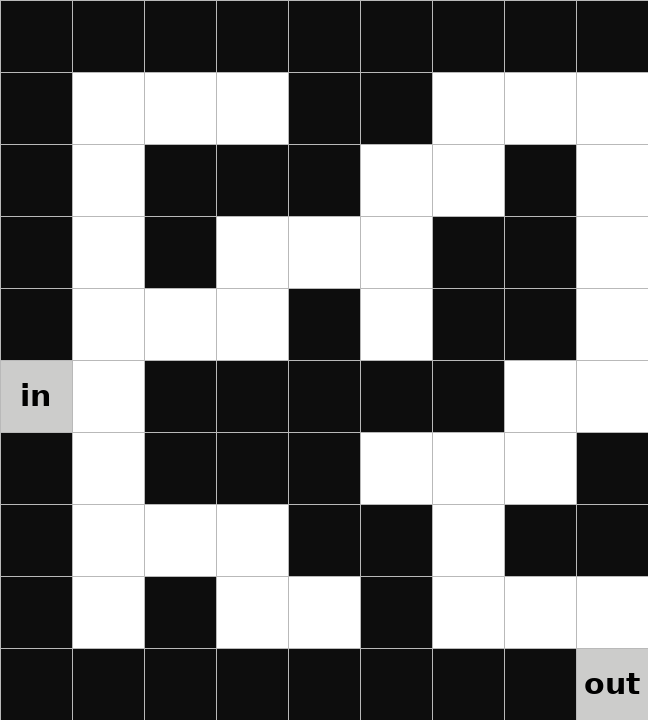
\includegraphics[width=0.42\textwidth]{figures/fig91_grid.png}

\medskip
\noindent\textbf{图 9.1\quad 一个小迷宫的例子，宝藏（出口）位于边缘}
\end{center}

但宝藏不一定非得在边缘上。图 9.2 展示了一个更大的迷宫，宝藏位于内部。

因为能看到迷宫的预览感觉很好，我们决定把自己的迷宫编码为图像。图像是表示二维（2D）网格的便捷方式，因为它有固定的大小。我们可以用颜色值编码某个网格元素是墙、路、入口还是宝藏。在前面的例子里，墙涂成黑色，路涂成白色。

% SOURCE_PDF_PAGE: 131
\begin{center}
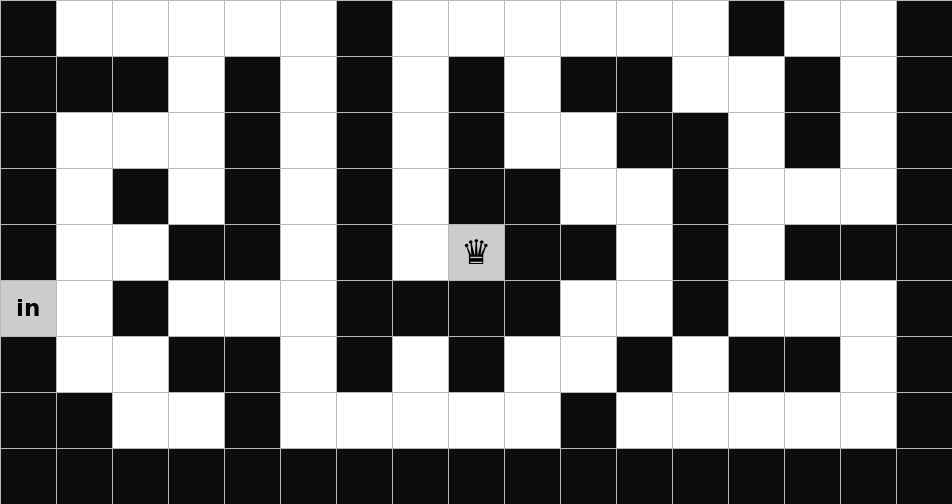
\includegraphics[width=0.60\textwidth]{figures/fig92_grid.png}

\medskip
\noindent\textbf{图 9.2\quad 宝藏位于内部的一个迷宫示例}
\end{center}

因为能看到迷宫的预览感觉很好，我们决定把自己的迷宫编码为图像。图像是表示二维网格的便捷方式，因为它有固定的大小。我们可以用颜色值编码某个网格元素是墙、路、入口还是宝藏。在前面的例子里，墙涂成黑色，路涂成白色。

\subsection{什么是图像？}

在计算机科学中，大多数 2D 图像属于两类之一：矢量图像或位图图像。矢量图像类似于数学实体——无论放大多少倍，线都没有粗细，点在屏幕上也不会显得更大，等等。可缩放矢量图形（SVG）是常见的矢量图像格式。

另一方面，位图图像（bitmap image），也称光栅图像（raster image），包含一个由图片元素组成的 2D 网格。这些图片元素（即像素）各自带有一个颜色。放大光栅图像时，像素只是被显示得更大。光栅图像的常见
% SOURCE_PDF_PAGE: 132
格式有便携式网络图形（PNG）和联合图像专家组（JPEG）。JPEG 图像提供有损压缩，这通常意味着存储信息所需的字节更少——但压缩的同时也可能修改图像。像素位置编码的通常是颜色，不过有时我们也用像素表达别的东西，例如热力图或密度（MRI 就是用图像来表示内部组织的），或者用于调色板——每种颜色都有特定含义（比如一幅世界地图，每个国家用不同颜色表示）。

因为我们想编码一个 2D 网格，光栅图像格式看起来完全够用。JPEG 的有损压缩可能导致像素颜色被改变，而我们需要精确的值来表示墙、路、入口和宝藏。因此，我们决定把图像编码为 PNG。

当然，Go 有一个用于图像操作的包，还有一个支持大多数常见图像格式的包：

\begin{shellcode}[]
> go doc image
package image // import "image"
[...]
type Image interface{ ... }
    func Decode(r io.Reader) (Image, string, error)
type Point struct{ ... }
type RGBA struct{ ... }
    func NewRGBA(r Rectangle) *RGBA
> go doc image.Point
type Point struct {
    X, Y int
}
    A Point is an X, Y coordinate pair. The axes increase right and down.
\end{shellcode}

我们在 \texttt{image} 包里看到的类型之一是 RGBAImage。它提供对 \texttt{RGBAAt(x, y)} 方法的访问，

% SOURCE_PDF_PAGE: 133
它让我们能取回图像中给定位置像素的颜色。

\subsection{迷宫的约束}

记住我们对求解器初始版本的约束：

\begin{itemize}
  \item 迷宫不会回环到自身。从入口到迷宫中任何一点都恰好只有一条路径。
  \item 生成的图像应当是使用 RGBA 颜色模型的 PNG 图像。
\end{itemize}

编写迷宫生成器时，还可以对从入口到宝藏的路径长度加一条复杂度约束，避免一眼看穿的答案。比如在我们的实现里，这条路径——也就是解——的长度必须至少是图像的高度加宽度。我们决定使用下列颜色，但你尽可以更有艺术气息、对色盲更友好：

\begin{itemize}
  \item 入口——暗色调（深蓝）
  \item 宝藏——亮色调（粉色）
  \item 墙——黑色
  \item 路——白色
\end{itemize}

现在我们有了生成的迷宫。开始解谜吧！

\section{迷宫求解器}

为了解迷宫，我们先打开生成的迷宫图像，然后探索可能的路径，同时把它们记录下来。到最后，我们会得到
% SOURCE_PDF_PAGE: 134
第一个凑合能用的版本（可能有点脏，但至少能跑），在找到宝藏时结束。

\subsection{准备工作}

跟往常一样，先建好模块并在根目录创建 \texttt{main.go}。因为这个项目是个简单的命令行工具，我们可以把 \texttt{main.go} 放在模块根目录，其余的放进 \texttt{internal} 文件夹。解迷宫的第一步是打开它。

\subsection{加载迷宫图像}

如前所述，我们希望输入 PNG 作为参数传给工具，同时传输出路径：

\begin{shellcode}[]
> maze-solver maze_10x10.png solution.png
\end{shellcode}

这意味着我们的 \texttt{main()} 要做的第一件事就是读这两个参数。

% SOURCE_PDF_PAGE: 135
\begin{gocode}[title={代码清单 9.1 \texttt{main.go}：读取参数}]
package main

import (
    "fmt"
    "log"
    "os"
)

func main() {
    if len(os.Args) != 3 { #1
        usage()
    }
    inputFile := os.Args[1] #2
    outputFile := os.Args[2]
    log.Printf("Solving maze %q and saving it as %q", inputFile, outputFile)
}

// usage displays the usage of the binary and exits the program.
func usage() {
    _, _ = fmt.Fprintln(os.Stderr, "Usage: maze_solver input.png output.png")
    os.Exit(1) #3
}

#1 Checks the number of arguments
#2 The name of the program is found at index 0 before the arguments.
#3 Exits the program with error code 1
\end{gocode}

\begin{codeannotations}
\item 检查参数数量
\item 程序名在参数之前的索引 0 处
\item 以错误码 1 退出程序
\end{codeannotations}

你已经可以运行它并检验各种场景了。接着我们打开包含迷宫的第一幅图像。此时可能发生的错误包括：根本没有文件，或图像不是 PNG。每种情况下，我们都要打印一条明确的错误。

这个操作可以用一句话概括，所以理所当然地把它放进一个函数。它接收字符串，返回 \texttt{*image.RGBA} 类型的图像。我们想要指针，因为最终我们要在写出通往宝藏的路径时修改图像。把这个函数写进一个新文件，它将包含文件 I/O 操作：

\begin{gocode}[]
func openMaze(imagePath string) (*image.RGBA, error)
\end{gocode}

就称新函数为 \texttt{openMaze} 吧。它将检查文件是否存在、打开它——别忘了 \texttt{defer} 对 \texttt{Close} 的调用——
% SOURCE_PDF_PAGE: 136
然后解码 PNG。最后一步通过调用 \texttt{image/png} 包的 \texttt{Decode} 完成，它接收一个 \texttt{io.Reader}，返回一个接口 \texttt{image.Image}。

然而不巧的是，\texttt{image.Image} 接口只提供一个访问像素值的方法——\texttt{At(x, y)}——它返回第 x 列与第 y 行交汇处像素的 \texttt{color.Color}。从普通 \texttt{image.Image} 的 \texttt{At} 返回的 \texttt{color.Color} 需要转换到 RGBA 颜色模型才可用。与其每次访问像素值都要调用 \texttt{At(x, y).RGBA()}，不如使用 \texttt{image.RGBA}——一个提供了非常方便的 \texttt{RGBAAt(x, y)} 方法的类型。为此，我们直接尝试把从文件解码出的 \texttt{image.Image} 类型断言为 \texttt{image.RGBA} 变量。

Go 提供了 \texttt{image.RGBA}，却不提供 \texttt{image.RGB}。因此本章把 RGBA 图像当作讨论对象会更简单，即便我们选择的颜色都是 100\% 不透明的。在 \texttt{main.go} 旁边创建一个名为 \texttt{imagefile.go} 的文件。

% SOURCE_PDF_PAGE: 137
\begin{gocode}[title={代码清单 9.2 \texttt{imagefile.go}：打开迷宫图像}]
package main

import (
    "fmt"
    "image"
    "image/png"
    "os"
)

// openMaze opens a RGBA png image from a path.
func openMaze(imagePath string) (*image.RGBA, error) {  #1
    f, err := os.Open(imagePath) #2
    if err != nil {
        return nil, fmt.Errorf("unable to open image %s: %w", imagePath, err)
    }
    defer f.Close()
    img, err := png.Decode(f) #3
    if err != nil {
        return nil, fmt.Errorf("unable to load input image from %s: %w",
            imagePath, err)
    }
    rgbaImage, ok := img.(*image.RGBA) #4
    if !ok {
        return nil, fmt.Errorf(
            "expected RGBA image, got %T", img) #5
    }
    return rgbaImage, nil
}

#1 Checks that the file exists
#2 Opens the file
#3 Tries decoding as a PNG
#4 Type asserts to *image.RGBA
#5 %T prints the type of a variable.
\end{gocode}

\begin{codeannotations}
\item 检查文件存在
\item 打开文件
\item 尝试按 PNG 解码
\item 类型断言为 \texttt{*image.RGBA}
\item \texttt{\%T} 打印变量的类型
\end{codeannotations}

图像到手了。别忘了在 main 里调用这个函数、妥善处理错误，并手动测试不同场景下的表现。

前面的代码里有两个错误场景很容易自动化测试：无法打开文件和无法加载 PNG 图像。要测试函数无法把它类型断言为 RGBA 图像，需要一幅不是按 RGBA 编码的 PNG 图像。我们在仓库的 \url{https://mng.bz/KGJX} 提供了这样一幅图。你应当会看到类似这样的输出：

% SOURCE_PDF_PAGE: 138
\begin{shellcode}[]
> go run . mazes/rgb.png solution.png
2023/10/16 18:26:28 INFO Solving maze "mazes/rgb.png" and saving it as
"solution.png"
ERROR: expected RGBA image, got *image.Paletted
exit status 1
\end{shellcode}

最后，还要处理``我们能检测到的文件打不开''时的 \texttt{os.Open} 错误。这种情况相当罕见——在 Unix 上，它要求你对某个目录有执行权限、却对该目录中的文件没有读权限。尽管如此，它可能发生，而知道它发生了会让我们很高兴。写个测试，然后我们就可以搭建求解部分了。

\subsection{加入求解器}

解迷宫将由一个专门的对象完成，它带有一个 \texttt{Solve()} 方法，并且可以通过传入图像来构造。为什么？这个对象将来能够持有各种设置，比如路径、墙、入口、宝藏和解（从入口到宝藏的路径）的颜色。你很快会看到，它还将持有 goroutine 之间通信的通道，以及最终的解。现在，先保持简单。

\subsubsection*{求解器结构}

Solver 是这个工具的心脏，值得住在专门的包里：\texttt{internal/solver}。记住——internal 里的包不能被你的模块之外的任何人使用。在 \texttt{internal/solver} 包中创建一个 \texttt{solver.go} 文件。

% SOURCE_PDF_PAGE: 139
\begin{gocode}[title={代码清单 9.3 \texttt{solver.go}：\texttt{Solver} 结构}]
package solver

import "image"

// Solver is capable of finding the path from the entrance to the treasure.
// The maze has to be a RGBA image.
type Solver struct {
    maze *image.RGBA
}
\end{gocode}

在继续之前，先定义这个对象的 API。它需要解迷宫并写出解的图像，如下一个清单所示。两个操作，因此是两个导出的方法。

\begin{gocode}[title={代码清单 9.4 \texttt{solver.go}：\texttt{Solve} API}]
// Solve finds the path from the entrance to the treasure.
func (s *Solver) Solve() error {
    return nil
}
\end{gocode}

\texttt{SaveSolution} 方法住在 \texttt{imagefile.go} 里，因为它属于图像操作的范畴。代码见下面的清单。

\begin{gocode}[title={代码清单 9.5 \texttt{imagefile.go}：保存解的 API}]
// SaveSolution saves the image as a PNG file
// with the solution path highlighted.
func (s *Solver) SaveSolution(outputPath string) error {
    return nil
}
\end{gocode}

\subsubsection*{NEW 函数}

实际上，我们的实现与 \texttt{image} 包高度绑定。为什么不把打开 PNG 图像这件事委托给一个 \texttt{New} 函数呢？反正我们迟早需要它。

把包含 \texttt{openImage} 函数的 \texttt{imagefile.go} 文件连同它的测试一起移到 solver 包，然后在一个叫 \texttt{New} 的新函数里调用 \texttt{openImage}。别忘了
% SOURCE_PDF_PAGE: 140
把 main 函数中先前对 \texttt{openImage} 的调用替换为对 \texttt{solver.New} 的调用。它接收路径作为参数，返回一个指向 Solver 的指针和一个错误，如下面的清单所示。注意，在一个文件里，我们倾向于把 \texttt{New} 函数和其他此类构造函数写在结构体定义之后。

\begin{gocode}[title={代码清单 9.6 \texttt{solver.go}：新建 \texttt{Solver}}]
// New builds a Solver by taking the path to the PNG maze, encoded in RGBA.
func New(imagePath string) (*Solver, error) {
    img, err := openMaze(imagePath)
    if err != nil {
        return nil, fmt.Errorf("cannot open maze image: %w", err)
    }
    return &Solver{maze: img}, nil
}
\end{gocode}

你现在的文件树应当像这样：

\begin{shellcode}[]
> tree
.
├── go.mod
├── internal
│   └── solver
│       ├── imagefile.go
│       └── solver.go
└── main.go
\end{shellcode}

此时，你甚至可以完成 main 函数的编写：按正确顺序构建 Solver 并调用其公开 API。用你喜欢的方式处理各种错误，但别忘了：命令行界面（CLI）工具出错时应当通过 \texttt{os.Exit(1)} 返回状态码 1。有任何疑问，请看 \url{https://mng.bz/9Yxj} 文件夹中的代码。

跑一跑你写的测试，提交，喝杯茶。下一节是本项目的心脏。

% SOURCE_PDF_PAGE: 141
\section{探索去也！}

上一节里，我们把迷宫图像加载进了内存。下一个目标是找到从入口到宝藏的路径，但首先得找到入口。

\subsection{寻找入口}

第一步相当直白，不过当然，如果一路上没有可学的东西，我们也不会写这本书了。把图像加载进内存并不意味着就能立刻解迷宫。首先，我们得知道怎么探索它。

\subsubsection*{调色板}

为了编码信息，迷宫生成器用像素在特定位置存储特定值。在我们的迷宫里，这些值表示墙、路、入口和宝藏。我们想把像素的颜色与这些特定值进行比较。RGBA 颜色在 \texttt{image/color} 包中以结构体表示，而结构体不能是常量，这意味着我们表示路、墙、入口和宝藏的参照色不能是常量。那我们怎么引用它们？有几个方案。

一种办法是把颜色声明为 solver 包里的全局变量。嗯，我们不喜欢全局变量：它们可能被误改、逃过所有测试的火眼金睛，然后整个行为变得完全无法解释。作为第一步它还行，但我们不希望它在生产环境里出现。

一个有意思的替代方案是创建一个调色板（palette）结构来持有所有不同的值。你可以在迷宫求解器运行时从
% SOURCE_PDF_PAGE: 142
配置文件加载调色板，但这超出了本章的范围。只要 main 包不需要修改这些值，我们就无需暴露这个结构。在 \texttt{internal/solver} 包里创建一个名为 \texttt{palette.go} 的文件。

\begin{gocode}[title={代码清单 9.7 \texttt{palette.go}：声明颜色列表}]
// palette contains the colours of the different types of pixels in our maze.
type palette struct {
    wall        color.RGBA
    path        color.RGBA #1
    entrance    color.RGBA #2
    treasure    color.RGBA
    solution    color.RGBA #3
}

#1 The color of the possible paths
#2 The pixel you're looking for
#3 Displays the solution
\end{gocode}

\begin{codeannotations}
\item 可能路径的颜色
\item 你要找的像素
\item 显示解
\end{codeannotations}

一个填好我们所选值的调色板结构可以由 \texttt{defaultPalette()} 函数返回，如代码清单 9.8 所示。相比全局变量的优势是：函数返回的值谁也改不了。遗憾的是，每次需要它都会创建一个新结构体，分配出需要垃圾回收的宝贵内存。一旦开始探索更大的迷宫，这就可能变得昂贵。

% SOURCE_PDF_PAGE: 143
\begin{gocode}[title={代码清单 9.8 \texttt{palette.go}：默认颜色函数}]
// defaultPalette returns the colour palette of our maze.
func defaultPalette() palette {
    return palette{
        wall:     color.RGBA{
            R: 0,   G: 0,   B: 0,   A: 255},  #1
        path:     color.RGBA{
            R: 255, G: 255, B: 255, A: 255}, #2
        entrance: color.RGBA{
            R: 0,   G: 191, B: 255, A: 255}, #3
        treasure: color.RGBA{
            R: 255, G: 0,   B: 128, A: 255}, #4
        solution: color.RGBA{
            R: 225, G: 140, B: 0,   A: 255}, #5
    }
}

#1 Black
#2 White
#3 Deep blue
#4 Pink
#5 Orange
\end{gocode}

\begin{codeannotations}
\item 黑色
\item 白色
\item 深蓝
\item 粉色
\item 橙色
\end{codeannotations}

我们实际做的，是把这些值作为求解这幅图像的设置保存在 Solver 结构里（见代码清单 9.9）。这很合理，因为另一个求解器面对另一幅图时，可以使用另一套颜色。

\begin{gocode}[title={代码清单 9.9 \texttt{solver.go}：带调色板的 \texttt{Solver}}]
type Solver struct {
    maze     *image.RGBA
    palette   palette
}
\end{gocode}

目前，你只需在 solver 包的 \texttt{New} 函数里用刚定义的 \texttt{defaultPalette()} 把这些颜色设为默认值。现在，循着指示牌去找入口吧。

\subsubsection*{像素定义}

我们将通过探索像素来穿越迷宫，像素由它们在 2D 图像上的坐标标识。既然要在这些 2D 网格中导航，就用 Go 提供的 \texttt{image.Point} 吧：

% SOURCE_PDF_PAGE: 144
\begin{gocode}[]
type Point struct {
    X, Y int
}
\end{gocode}

关于像素，有一点可以轻易预见：我们需要找到它的开放邻居——与它正交相连、带有路颜色的像素。如果像素能告诉我们自己邻居的坐标，事情会容易得多。由于迷宫的实现方式，我们不想包含对角相邻的邻居。在 \texttt{internal/solver} 包中创建一个名为 \texttt{neighbours.go} 的文件，编写 \texttt{neighbours} 函数。

\begin{gocode}[title={代码清单 9.10 \texttt{neighbours.go}：像素的坐标}]
package solver

import "image"

// neighbours returns an array of the 4 neighbours of a pixel.
// Some returned positions may be outside the image.
func neighbours(p image.Point) [4]image.Point {
    return [...]image.Point{
        {p.X, p.Y + 1}, #1
        {p.X, p.Y - 1}, #2
        {p.X + 1, p.Y}, #3
        {p.X - 1, p.Y}, #4
    }
}

#1 One pixel down
#2 One pixel up
#3 One pixel to the right
#4 One pixel to the left
\end{gocode}

\begin{codeannotations}
\item 下一个像素
\item 上一个像素
\item 右侧一个像素
\item 左侧一个像素
\end{codeannotations}

\begin{infobox}{注意}
在这个函数里，我们返回的是一个数组。这里的 \texttt{[...]image.Point} 等价于 \texttt{[4]image.Point}，后者是一个数组（数组长度在编译期计算）。使用数组是个小优化：它更可能被分配在栈上而不是堆上。
\end{infobox}

这个函数没有任何东西保证邻居在图像之内。比如，位于 (0, 0) 的左上角像素有两个邻居在图像之外。我们可以
% SOURCE_PDF_PAGE: 145
在这里加一道安全网，或者规定图像的边缘一律不予探索。

另一种思路是想想我们会怎么使用这些邻居。稍后在代码里，我们要检查它们代表迷宫中可探索的一段、一堵墙、宝藏，还是我们编码的其他信息。为此，必须查看每个邻居的 \texttt{RGBAAt(position)} 返回值。查一下它的实现就会发现：当位置在图像之外时，\texttt{RGBAAt} 返回零值。这意味着让 \texttt{neighbours} 返回超出图像边界的点是安全的。

API 不保证的另一件事是邻居的顺序。我们可以从上方开始顺时针排列，也可以狂野一点直接打乱。这意味着编写测试正是使用 \url{https://github.com/stretchr/testify} 框架及其 \texttt{assert.ElementsMatch} 函数的绝佳时机。

\subsubsection*{找到入口的像素}

回到 \texttt{solver.go} 文件，创建函数 \texttt{findEntrance}。我们必须扫描整幅图像，找到一个具有入口颜色的像素。要检查每个像素的值，图像处理中的一个常见做法是按行优先顺序（row-major order）使用两层嵌套循环：外层循环遍历图像的各行，内层循环遍历行中的各列。这类似于某些语言（如英语或提菲纳格字母）书写文本的方式：从最左写到最右，然后换行，再从最左开始。

之所以是这种特定模式，是因为图像格式往往以扫描线（scanline）格式存储像素值，
% SOURCE_PDF_PAGE: 146
图像中水平相邻的像素被存储在相邻的内存位置。想到大多数图像格式的开发者都以英语为母语，这一点就好理解了。

大多数时候，我们迷宫的第一个像素位于 (0, 0)——左上角。但如果我们看的是图像的一个子区域，我们的``左上角''可能在别的位置。这里可以通过 \texttt{image.RGBA} 类型的 \texttt{Bounds()} 方法访问迷宫的边界。它返回定义图像包围盒的两个点：\texttt{Min} 和 \texttt{Max} 字段。

\begin{gocode}[title={代码清单 9.11 \texttt{solver.go}：寻找入口}]
// findEntrance returns the position of the maze entrance on the image.
func (s *Solver) findEntrance() (image.Point, error) {
    for row := s.maze.Bounds().Min.Y; row < s.maze.Bounds().Max.Y; row++ {
        for col := s.maze.Bounds().Min.X; col < s.maze.Bounds().Max.X; col++
    {
            if s.maze.RGBAAt(col, row) == s.palette.entrance {
                return image.Point{X: col, Y: row}, nil #1
            }
        }
    }
    return image.Point{}, fmt.Errorf("entrance position not found")
}

#1 Returns as soon as we find an entrance
\end{gocode}

\begin{codeannotations}
\item 一找到入口就返回
\end{codeannotations}

回到 \texttt{Solve} 方法，我们可以调用它来确定起点，如下面的清单所示。

\begin{gocode}[title={代码清单 9.12 \texttt{solver.go}：在 \texttt{Solve} 中调用 \texttt{findEntrance}}]
// Solve finds the path from the entrance to the treasure.
func (s *Solver) Solve() error {
    entrance, err := s.findEntrance()
    if err != nil {
        return fmt.Errorf("unable to find entrance: %w", err)
    }
    log.Printf("starting at %v", entrance))
    return nil
}
\end{gocode}

% SOURCE_PDF_PAGE: 147
如果没有入口怎么办？确保在测试中覆盖各种情形。也许我们希望迷宫只有一个入口。如果你写测试时遇到困难，可以在 \url{https://mng.bz/jpMa} 的文件里找到我们的测试用例，所有场景使用的迷宫图像都放在本书仓库的 \texttt{internal/solver/testdata} 下（\url{https://mng.bz/GeMv}）。图 9.3 展示了一个已识别出入口的迷宫。

\begin{center}
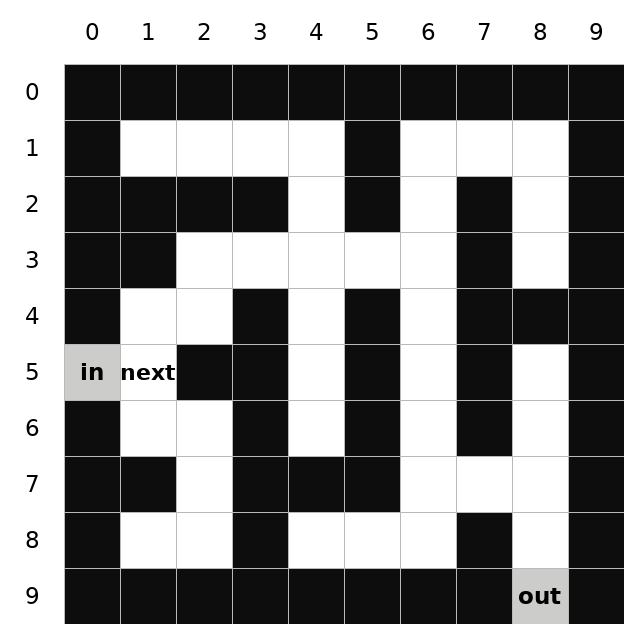
\includegraphics[width=0.44\textwidth]{figures/fig93_grid.png}

\medskip
\noindent\textbf{图 9.3\quad 标出入口和下一个像素的迷宫}
\end{center}

我们已经从入口踏进迷宫并探索了一个像素。现在需要探索下一个（些）像素，才能抵达宝藏。

\subsection{传达新的可行路径}

解迷宫的优化算法很多，但大多采用迭代式的方法——在每个转角左转、前往既离入口最近又未探索过的位置，等等。
% SOURCE_PDF_PAGE: 148
每当遇到一个岔路口，都必须做出决策：先左、再右、然后直行？本章我们用一个问句回答这个问题：为什么不同时试所有方向？这就需要并行编程，在 Go 中用 goroutine 实现。每次发现路径分岔，我们会想沿着其中一个可能方向继续，并为其他方向启动 goroutine。使用 goroutine 意味着我们可以把其他方向的探索委托出去，专注走完当前分支，直到抵达宝藏或死胡同。

使用 goroutine 可以提升性能——让找到解的速度更快——但这并非保证。启动 goroutine 需要时间，与它们通信还会增加额外开销。通常，对非常快的任务来说 goroutine 并非必要。在我们的例子里，每个 goroutine 的作用范围都无法确定：我们不知道它何时结束，那不妨给它一个机会。

可以确定的是，使用 goroutine 会增加 CPU 的使用。在图 9.4 中，我们要寻找宝藏（$\mu$）。goroutine 代达罗斯（$\delta$）从 A5 出发，然后到 B5，需要分岔。第二个 goroutine 忒修斯（$\theta$）从 B6 接手，而 $\delta$ 继续走向 B4、C4 等等。只要迷宫里没有环，代达罗斯和忒修斯在探索迷宫时就不会相遇，这意味着代达罗斯完全不需要知道忒修斯的存在。

% 图 9.4：代达罗斯与忒修斯的并发探索（依原书重绘）
\begin{center}
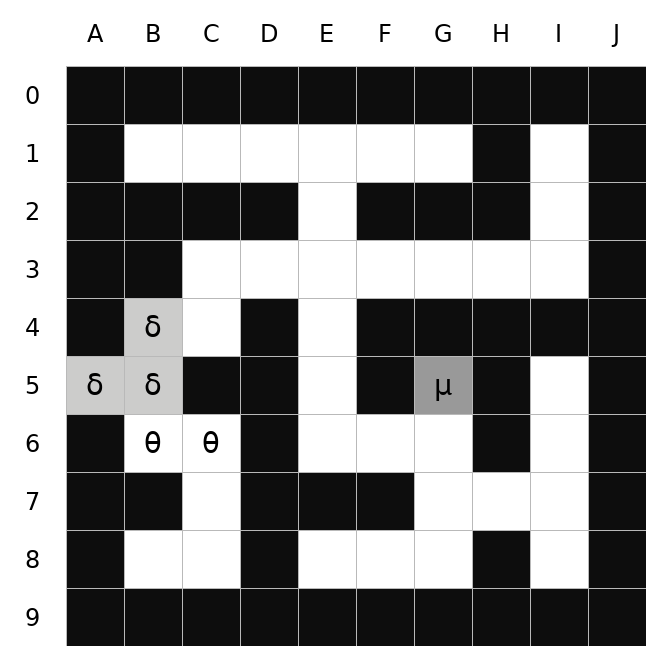
\includegraphics[width=0.44\textwidth]{figures/fig94_grid.png}

\medskip
\noindent\textbf{图 9.4\quad 由不同 goroutine 进行的探索}
\end{center}

% SOURCE_PDF_PAGE: 149
从那里开始，两个 goroutine 继续探索，不断启动新的探索者。抵达宝藏的探索过程可能看起来像图 9.5（每个 goroutine 探索过的路径用不同的希腊字母表示）。

% 图 9.5：一次可能的事件序列的探索（依原书重绘）
\begin{center}
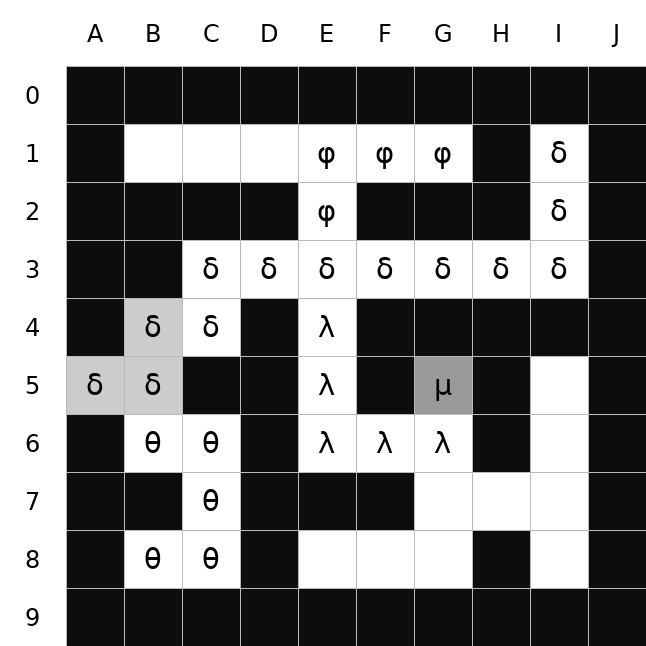
\includegraphics[width=0.44\textwidth]{figures/fig95_grid.png}

\medskip
\noindent\textbf{图 9.5\quad 表示一次可能的事件序列的探索}
\end{center}

\begin{infobox}{注意}
goroutine 之间的通信是通道的用途所在。
\end{infobox}

找到入口的位置后，我们的 \texttt{Solve} 函数负责从那里开始，发起对迷宫的探索。一旦有新路径要探索，我们就希望求解器开始对那条分支的探索。每个探索者负责通过通道向求解器通报新分支，% SOURCE_PDF_PAGE: 150
求解器则监听这些通知。由此我们明白：需要给求解器添加两个新方法——第一个探索一条路径，不妨叫 \texttt{explore}；第二个负责监听各条分支，就叫它 \texttt{listenToBranches} 吧。我们的求解器通过向通道发送一条消息来发起对迷宫的探索，而 \texttt{listenToBranches} 方法正在监听这个通道。

% SOURCE_PDF_PAGE: 151
\texttt{listenToBranches} 函数读出第一条消息，为一个从 A5 出发的路径创建 goroutine——就是我们叫作代达罗斯（$\delta$）的那个。图 9.6 展示了以下事件的示意图。代达罗斯查看 A5 的邻居：只有 B5 合格。这个 goroutine 把 B5 纳入自己已探索的路径，再查看 B5 的邻居，发现 B4 和 B6 是值得探索的候选。我们这位探索者 goroutine——代达罗斯——把通往 B6 的路径发送到通道，继续探索 B4、C4 等等。通道的监听者读出代达罗斯发来的消息，启动一个新的 goroutine——忒修斯（$\theta$）——它接着走向 C6、C7 等等，直到撞见死胡同而结束。与此同时，代达罗斯已抵达 E3，面临三条新的探索路径。它（随机地）选择继续走自己的路（D3、E3、C3），把通向 E2 和 E4 的路径发送到通道，监听者又启动了两个新 goroutine，$\lambda$ 和 $\varphi$。

当然，在这个场景里，请对文中的语法时态持保留态度——因为取决于你的架构和 CPU 随机决定的重新调度，未来、现在与过去可能每次运行都不一样。动手实现它有助于我们更好地理解这些细节。

% SOURCE_PDF_PAGE: 152
% 图 9.6：Solve 中事件的先后顺序（依原书重绘的时序图）
\begin{center}
\begin{tikzpicture}[
  x=1cm, y=1cm,
  part/.style={draw=PocketTealDark, thick, rounded corners=1.2mm, fill=PocketMist,
               font=\ttfamily\scriptsize, inner sep=3pt, minimum height=5.2mm},
  msg/.style={-{Stealth[length=2.2mm]}, thick},
  lbl/.style={font=\ttfamily\tiny, above=1.3pt, midway, fill=white, inner sep=0.7pt},
  lifeline/.style={dashed, black!55, thick},
  act/.style={draw=black!70, fill=white, thick},
]
% Six participants only: the E4 branch is intentionally launched off-chart,
% matching the source sequence diagram rather than inventing a seventh lifeline.
\def\axS{-0.35} % Solve
\def\axL{2.10}  % listenToBranches
\def\axE{4.35}  % explore
\def\axD{6.10}  % for loop delta
\def\axT{8.05}  % for loop theta
\def\axF{10.05} % for loop varphi

% lifelines
\foreach \x in {\axS,\axL,\axE,\axD,\axT,\axF}
  {\draw[lifeline] (\x,-0.50) -- (\x,-13.05);}

% participant boxes (top and bottom)
\foreach \x/\name in {\axS/{Solve}, \axL/{listenToBranches}, \axE/{explore},
                      \axD/{for~loop $\delta$}, \axT/{for~loop $\theta$}, \axF/{for~loop $\varphi$}}
  {\node[part] at (\x,0) {\name}; \node[part] at (\x,-13.45) {\name};}

% activations
\filldraw[act] (\axL-0.08,-0.62) rectangle (\axL+0.08,-12.72);
\filldraw[act] (\axE-0.08,-1.08) rectangle (\axE+0.08,-1.78);
\filldraw[act] (\axD-0.08,-1.68) rectangle (\axD+0.08,-12.82);
\filldraw[act] (\axT-0.08,-3.98) rectangle (\axT+0.08,-11.92);
\filldraw[act] (\axF-0.08,-7.92) rectangle (\axF+0.08,-12.02);

% Solve starts the listener.
\draw[msg] (\axS,-0.62) -- (\axL,-0.62);

% Listener asks explore to begin at A5, then explore launches Daedalus (delta).
\draw[msg] (\axL,-1.15) -- node[lbl]{go $\delta$ on A5} (\axE,-1.15);
\draw[msg] (\axE,-1.68) -- (\axD,-1.68);

% B5 and B4 are explored by delta (not by the explore dispatcher).
\node[font=\ttfamily\scriptsize,anchor=south west] at (\axD+0.18,-2.05) {B5};
\draw[thick] (\axD+0.08,-2.02) -- (\axD+0.78,-2.02) -- (\axD+0.78,-2.34);
\draw[msg] (\axD+0.78,-2.34) -- (\axD+0.08,-2.34);
\node[font=\ttfamily\scriptsize,anchor=south west] at (\axD+0.18,-2.66) {B4};
\draw[thick] (\axD+0.08,-2.63) -- (\axD+0.78,-2.63) -- (\axD+0.78,-2.95);
\draw[msg] (\axD+0.78,-2.95) -- (\axD+0.08,-2.95);

% Delta publishes the B6 branch; the listener starts Theseus (theta).
\draw[msg] (\axD,-3.38) -- node[lbl]{A5, B5, B6} (\axL,-3.38);
\draw[msg] (\axL,-3.98) -- node[lbl]{go $\theta$ on A5, B5, B6} (\axT,-3.98);

% Concurrent exploration on delta and theta.
\node[font=\ttfamily\scriptsize,anchor=south west] at (\axD+0.18,-4.48) {C4, \ldots, E3};
\draw[thick] (\axD+0.08,-4.45) -- (\axD+0.98,-4.45) -- (\axD+0.98,-4.77);
\draw[msg] (\axD+0.98,-4.77) -- (\axD+0.08,-4.77);

\node[font=\ttfamily\scriptsize,anchor=south west] at (\axT+0.18,-4.72) {C6};
\draw[thick] (\axT+0.08,-4.69) -- (\axT+0.78,-4.69) -- (\axT+0.78,-5.01);
\draw[msg] (\axT+0.78,-5.01) -- (\axT+0.08,-5.01);
\node[font=\ttfamily\scriptsize,anchor=south west] at (\axT+0.18,-5.48) {C7};
\draw[thick] (\axT+0.08,-5.45) -- (\axT+0.78,-5.45) -- (\axT+0.78,-5.77);
\draw[msg] (\axT+0.78,-5.77) -- (\axT+0.08,-5.77);
\node[font=\ttfamily\scriptsize,anchor=south west] at (\axT+0.18,-6.24) {C8};
\draw[thick] (\axT+0.08,-6.21) -- (\axT+0.78,-6.21) -- (\axT+0.78,-6.53);
\draw[msg] (\axT+0.78,-6.53) -- (\axT+0.08,-6.53);

% At E3 delta publishes the E2 and E4 branches.
\draw[msg] (\axD,-6.82) -- node[lbl]{A5, B5, \ldots, E3, E2} (\axL,-6.82);
\draw[msg] (\axD,-7.38) -- node[lbl]{A5, B5, \ldots, E3, E4} (\axL,-7.38);

% The listener starts varphi on E2; the E4 branch is another goroutine outside this chart.
\draw[msg] (\axL,-7.95) -- node[lbl]{go $\varphi$ on A5, B5, \ldots, E3, E2} (\axF,-7.95);
\draw[msg,dashed] (\axL,-8.50) -- node[lbl]{go A5, B5, \ldots, E3, E4} (11.28,-8.50);

% Later events on the three visible worker goroutines.
\node[font=\ttfamily\scriptsize,anchor=south west] at (\axD+0.18,-9.13) {F3};
\draw[thick] (\axD+0.08,-9.10) -- (\axD+0.78,-9.10) -- (\axD+0.78,-9.42);
\draw[msg] (\axD+0.78,-9.42) -- (\axD+0.08,-9.42);

\node[font=\ttfamily\scriptsize,anchor=south west] at (\axT+0.18,-9.28) {B8};
\draw[thick] (\axT+0.08,-9.25) -- (\axT+0.78,-9.25) -- (\axT+0.78,-9.57);
\draw[msg] (\axT+0.78,-9.57) -- (\axT+0.08,-9.57);

\node[font=\ttfamily\scriptsize,anchor=south west] at (\axF+0.18,-9.43) {E1};
\draw[thick] (\axF+0.08,-9.40) -- (\axF+0.78,-9.40) -- (\axF+0.78,-9.72);
\draw[msg] (\axF+0.78,-9.72) -- (\axF+0.08,-9.72);

% Varphi publishes the branch through D1 back to the listener.
\draw[msg] (\axF,-10.25) -- node[lbl]{A5, \ldots, E1, D1} (\axL,-10.25);

\node[font=\ttfamily\scriptsize,anchor=south west] at (\axD+0.18,-10.92) {G3};
\draw[thick] (\axD+0.08,-10.89) -- (\axD+0.78,-10.89) -- (\axD+0.78,-11.21);
\draw[msg] (\axD+0.78,-11.21) -- (\axD+0.08,-11.21);

\node[font=\ttfamily\scriptsize,anchor=south west] at (\axT+0.18,-10.92) {Dead end.};
\draw[thick] (\axT+0.08,-10.89) -- (\axT+1.02,-10.89) -- (\axT+1.02,-11.21);
\draw[msg] (\axT+1.02,-11.21) -- (\axT+0.08,-11.21);
\draw[thick,black] (\axT-0.22,-11.52) -- (\axT+0.22,-11.78)
                   (\axT-0.22,-11.78) -- (\axT+0.22,-11.52);

\node[font=\ttfamily\scriptsize,anchor=south west] at (\axF+0.18,-11.08) {F1};
\draw[thick] (\axF+0.08,-11.05) -- (\axF+0.78,-11.05) -- (\axF+0.78,-11.37);
\draw[msg] (\axF+0.78,-11.37) -- (\axF+0.08,-11.37);

% Listener returns to Solve after the winning branch is reported.
\draw[msg] (\axL,-12.55) -- (\axS,-12.55);
\end{tikzpicture}

\medskip
\noindent\textbf{图 9.6\quad \texttt{Solve} 中事件的先后顺序}
\end{center}

为了让代达罗斯启动一个自主的 goroutine，让它能够从 B6 继续探索路径，它只需把到目前为止的路径传达给忒修斯和那个抵达宝藏的 goroutine。仅此而已。它们需要知道经由已探索像素抵达此处所走的路径，我们可以把它表示为 \texttt{image.Point} 的链表，如代码清单 9.13 所示。创建 \texttt{internal/solver/path.go} 文件，加上 \texttt{path} 结构。

% SOURCE_PDF_PAGE: 153
\begin{gocode}[title={代码清单 9.13 \texttt{path.go}：用链表存储迄今为止的路径}]
package solver

import "image"

// path represents a route from the entrance of the maze up to a position.
type path struct {
    previousStep *path
    at           image.Point
}
\end{gocode}

给 Solver 加一个字段，它是一个通道，其消息是指向 \texttt{path} 的指针。

\begin{gocode}[title={代码清单 9.14 \texttt{solver.go}：给 \texttt{Solver} 结构添加通道}]
type Solver struct {
    maze           *image.RGBA
    palette        palette
    pathsToExplore chan *path #1
}

#1 A channel that carries linked lists of explored pixels
\end{gocode}

\begin{codeannotations}
\item 一个承载已探索像素链表的通道
\end{codeannotations}

这里就是 goroutine 发布新待探索路径的地方，也是 \texttt{listenToBranches} 方法监听并启动新探索 goroutine 的地方。该方法将在 9.3.4 节加入，因为常识告诉我们：只要通道还开着，就不能从一个还没写入任何东西的通道里读取。

\subsection{记录已探索的路径}

考虑到这个程序的目的是告诉我们如何从一点走到另一点，每探索一个新像素时，我们都需要知道自己是怎么到这里的。我们不能像法国童话里的小拇指（Hop-o'-My-Thumb）那样一路丢石子，但计算机的内存完全可以为我所用。

% SOURCE_PDF_PAGE: 154
\subsubsection*{每个 goroutine 的行为}

我们来写 \texttt{explore} 函数：它接收一条路径作为参数并探索它。这个函数会一直运行，直到找到死胡同或宝藏，并把它不走的分支发布到通道上。这个函数包含每个 goroutine 要做的事。

第一版里，如果找到了宝藏，我们先只打印一条消息，然后用 \texttt{return} 停止探索。这个后面再回来处理。

我们选择把这个函数放进 solver 包中一个专门的文件 \texttt{explore.go}，如代码清单 9.15 所示。这个函数足够重要，我们会经常回头调试它。

% SOURCE_PDF_PAGE: 155
\begin{gocode}[title={代码清单 9.15 \texttt{explore.go}：探索一条路径}]
package solver

import (
    "image"
    "log"
)

// explore one path and publish to the s.pathsToExplore channel
// any branch we discover that we don't take.
func (s *Solver) explore(pathToBranch *path) {
    if pathToBranch == nil {
        // This is a safety net. It should be used, but when it's needed,
        // at least it's there.
        return
    }
    pos := pathToBranch.at #1
    for {
// We know we'll have up to 3 new neighbours to explore.#2
        candidates := make([]image.Point, 0, 3)
        for _, n := range neighbours(pos) { #3
            if  pathToBranch.isPreviousStep(n){ #4
                // Let's not return to the previous position
                continue
            }
            // Look at the colour of this pixel.
            // RGBAAt returns a color.RGBA{} zero value if the pixel is
            // outside the bounds of the image.
            switch s.maze.RGBAAt(n.X, n.Y) { #5
            case s.palette.treasure:
                log.Printf("Treasure found at %v!", n)
                return
            case s.palette.path: #6
                candidates = append(candidates, n)
            }
        }
        if len(candidates) == 0 {
            log.Printf("I must have taken the wrong turn at position %v.",
                pos)
            return
        }
        // See below
    }
}

// isPreviousStep returns true if the given point is
// the previous position of the path.
func (p path) isPreviousStep(n image.Point) bool {
    return p.previousStep != nil && p.previousStep.at == n
}

#1 This is the pixel we're at.
#2 Forever until we break out or find a dead end
#3 Peeks in each direction for path pixels
% SOURCE_PDF_PAGE: 156
#4 This is where we came from.
#5 Checks the color of the neighbor
#6 This is a valid candidate.
\end{gocode}

\begin{codeannotations}
\item 这就是我们所在的像素
\item 直到 break 或找到死胡同才结束
\item 向各个方向探测路径像素
\item 这是我们来的地方
\item 检查邻居的颜色
\item 这是一个有效候选
\end{codeannotations}

注意，到目前为止，邻居只能是墙、路、入口或宝藏。入口已经被跳过，因为它是前一个像素；墙我们无能为力。这就是 switch 里只有两个 case 的原因——而且我们没有添加空的 default 分支：我们要么找到宝藏，要么找到下一个可探索的位置，别的东西都无趣。很重要的一点是：在寻找合格邻居时，我们不想原路返回、退回前一个位置。那会导致 goroutine 无休止地创建、程序崩溃。我们会在 9.6.1 节探讨阻止这种情况的方法。

然后有两种情况要考虑：要么没有下一个像素可探索——那就是死胡同；要么有下一个像素可探索，那就得向监听的 goroutine 发消息。死胡同的情形，我们打印一条日志消息来了解发生了什么，此外无事可做。我们退出循环，goroutine 结束自己的执行。

\subsubsection*{分岔}

如果确实有一个或多个待探索的像素候选，我们给自己留一个（在我们的例子里是第一个，\texttt{candidates[0]}），并把其余路径发送到通道上，如下面的清单所示。然后，我们继续把探索向前推进一步。

% SOURCE_PDF_PAGE: 157
\begin{gocode}[title={代码清单 9.16 \texttt{explore.go}：继续探索}]
for _, candidate := range candidates[1:] { #1
    branch := &path{previousStep: pathToBranch, at: candidate}
    s.pathsToExplore <- branch #2
}
pathToBranch = &path{
    previousStep: pathToBranch,
    at: candidates[0]} #3
pos = candidates[0]

#1 Ignores candidates[0]
#2 Publishes the path leading to the branch
#3 Continues exploring
\end{gocode}

\begin{codeannotations}
\item 忽略 \texttt{candidates[0]}
\item 发布通往分支的路径
\item 继续探索
\end{codeannotations}

这是个相当长的函数。我们可以通过抽取逻辑片段来重构。循环通常是个好候选，因为它们可以用一句话概括，在逻辑上是一个单元。看看我们的选项：

\begin{itemize}
  \item 抽取大无限循环的内部。这个选项要返回的变量太多：下一个位置、下一个``前一个''位置、是否退出的信号，可能还有一个错误。
  \item 抽取第一部分，即我们寻找候选的部分。这是我们选择在成功时退出的地方。可行，但不太容易。
  \item 抽取第二个 switch，即我们查看候选的部分。这种情况下，我们也会在死胡同时退出。我们可以把发布循环抽出来，但为了三行代码，代码真的会变得更容易理解吗？
\end{itemize}

先保持现状，看看写测试是不是过于复杂。常言道，因为我们想尽可能隔离逻辑，测试往往比代码本身更复杂一点，并且至少需要同样的概念，所以我们打算再稍等片刻。不过，可别养成习惯。

% SOURCE_PDF_PAGE: 158
\subsection{等待未探索的路径并启动 goroutine}

探索时，我们需要一个函数来监听通道，并为通道里的每条消息启动一个新 goroutine。它不必复杂：对通道里的每条消息，调用 \texttt{explore}，如代码清单 9.17 所示。

Go 中监听发布到通道的所有消息的关键字是 \texttt{range}，与切片或映射上的用法完全一样。对通道使用 \texttt{range} 是阻塞的，也就是说，只要 \texttt{close(s.pathsToExplore)} 没被调用，这个函数就会一直等待通道上发布的消息。

\begin{gocode}[title={代码清单 9.17 \texttt{explore.go}：监听通道}]
// listenToBranches creates a new goroutine for each branch published in
// s.pathsToExplore.
func (s *Solver) listenToBranches() {
    for p := range s.pathsToExplore {
        go s.explore(p)
    }
}
\end{gocode}

这是一个非常短的实现；它能工作，但对 goroutine 来说有个隐患。我们知道它们何时开始，却不知道何时结束。这里，我们没有追踪各个 goroutine（也没追踪它们的数量），这意味着程序可能在它们还在运行、还在占用内存和 CPU 时就结束了。在我们的代码被算作正确之前，需要先修复这一点。

但先让程序跑起来。启动探索要做的最后一件事是发布第一条消息。为了启动第一个 goroutine——我们在例子里叫它代达罗斯的那个——只需要把入口发布到通道并开始监听。

回到 \texttt{Solve} 函数。它知道入口像素的位置，我们可以把它发布出去：

% SOURCE_PDF_PAGE: 159
\begin{gocode}[]
s.pathsToExplore <- &path{previousStep: nil, at: entrance}
\end{gocode}

别忘了在那之后调用监听函数 \texttt{listenTobranches}，然后试着运行程序。有报错吗？你应当会看到。我们现在得到的是：

\begin{shellcode}[]
fatal error: all goroutines are asleep - deadlock!
goroutine 1 [chan send (nil chan)]:
learngo/09/maze/internal/solver.(*Solver).Solve(0x1400009c180)
\end{shellcode}

我们正试图对一个 nil 通道又写又读。在 \texttt{New} 函数里初始化通道，然后像下面这样再试：

\begin{gocode}[]
pathsToExplore: make(chan *path),
\end{gocode}

还是同样的问题。我们选了无缓冲通道，在读取之前向它发送消息会一直触发致命错误。

\begin{infobox}{注意}
对无缓冲通道的发送操作会阻塞发送的 goroutine，直到同一通道上发生对应的接收。此时，值被传递，两个 goroutine 才能继续。关于无缓冲通道的更多内容，请参阅 Alan A. A. Donovan 与 Brian W. Kernighan 的《The Go Programming Language》（Addison-Wesley Professional，2015）。
\end{infobox}

在开始读取之前，我们不能写无缓冲通道。作为替代，可以给通道一个单值缓冲。一个值就够了，因为写完这个值之后，我们的主 goroutine 会永远监听：

\begin{gocode}[]
pathsToExplore: make(chan *point, 1),
\end{gocode}

或者，如果我们当初建的是无缓冲通道 \texttt{make(chan *point)}，\texttt{Solve} 函数里对通道的写入也可以放进一个 goroutine 里做：

% SOURCE_PDF_PAGE: 160
\begin{gocode}[]
go func() { s.pathsToExplore <- &path{previousStep: nil, at: entrance} }()
\end{gocode}

如你所见，只要日志到处都是，缓冲大小取 1 就足以解出一个小迷宫，但程序最终仍会以死锁收场。如前所说，主 goroutine 会永远监听，即使所有子例程早已停止发布。Go 会注意到这一点，稍过片刻以死锁错误结束执行。我们需要一种办法告诉监听方法停下来。

\subsection{别听了，找到了：简短版}

当某个 goroutine 找到宝藏时，它需要把通往宝藏的路径存在某个地方，并设法告诉所有其他 goroutine 别再找了，同时告诉监听者别再听了。我们先实现一个快速版本，以便尽快看到漂亮的东西、看到它的局限，再找出更好的方案。

几页之前我们抄了个小近道，就在找到宝藏的地方。此时，我们需要把像素路径保存在 \texttt{SaveSolution} 函数能找到的地方。多数情况下，把它放进 Solver 里就足够好了，如代码清单 9.18 所示。另外，它还可以充当一个旗标，告诉各个 goroutine 宝藏已经找到、可以停止寻找了。

\begin{gocode}[title={代码清单 9.18 \texttt{solver.go}：添加解}]
type Solver struct {
    maze         *image.RGBA
    palette       palette
    pathsToExplore   chan *path
    solution *path #1
}

#1 Saves the solution
\end{gocode}

\begin{codeannotations}
\item 保存解
\end{codeannotations}

在 \texttt{explore} 函数里，给这个字段赋值只需要一行。回到那个 switch，如后面的清单所示。

% SOURCE_PDF_PAGE: 161
\begin{gocode}[title={代码清单 9.19 \texttt{explore.go}：保存解}]
case s.palette.treasure:
    s.solution = &path{previousStep: pathToBranch, at: n} #1
    log.Printf("Treasure found at %v!", n))
    return

#1 Adds the treasure to the path
\end{gocode}

\begin{codeannotations}
\item 把宝藏加进路径
\end{codeannotations}

等等——任何 goroutine 都可能写 \texttt{s.solution}，那怎么避免制造数据竞争？加一个互斥锁来保护自己吧。这个互斥锁是 Solver 结构的新字段。下面的清单展示我们在 treasure 这个 case 里如何使用它。

\begin{gocode}[title={代码清单 9.20 \texttt{explore.go}：用互斥锁保存解}]
case s.palette.treasure:
    s.mutex.Lock()
    defer s.mutex.Unlock() #1
    if s.solution == nil {
        s.solution = &path{previousStep: pathToBranch, at: n}
        log.Printf("Treasure found at %v!", n))
    }
    return

#1 It's OK to defer despite being in a loop because this case always
returns.
\end{gocode}

\begin{codeannotations}
\item 尽管处在循环里，这里 \texttt{defer} 也没问题，因为这个 case 总会返回
\end{codeannotations}

接着，为了告诉其他 goroutine 停下来，我们把这个解字段当作旗标用。诚然这不是什么好方案，但它够快。因为要在好几处检查解是否已找到，我们可以写一个函数。

% SOURCE_PDF_PAGE: 162
\begin{gocode}[title={代码清单 9.21 \texttt{explore.go}：停止监听新消息}]
func (s *Solver) listenToBranches() {
    for p := range s.pathsToExplore {
        go s.explore(p)
        if s.solutionFound() { #1
            return
        }
    }
}

// solutionFound returns whether the solution was found.
func (s *Solver) solutionFound() bool {
    s.mutex.Lock()
    defer s.mutex.Unlock()
    return s.solution != nil
}

#1 Stops listening if the treasure is found
\end{gocode}

\begin{codeannotations}
\item 找到宝藏就停止监听
\end{codeannotations}

在 \texttt{explore} 函数里还有一个可以叫停的无限循环。我们可以改造它，让它在解被找到时停下来，如下面的清单所示。

\begin{gocode}[title={代码清单 9.22 \texttt{explore.go}：停止探索一条路径}]
func (s *Solver) explore(pathToBranch []image.Point) {
    //...
    for !s.solutionFound() { #1
        candidates := ...
\end{gocode}

\begin{codeannotations}
\item 当解尚未被找到时
\end{codeannotations}

跑一跑。死锁止住了吗？取决于输入迷宫的复杂度，可能止住了，也可能没有，因为我们的方案很凑合。在正式修好它之前，是时候开始把测试自动化了。

\subsection{测试单个 goroutine 的逻辑}

我们可以在一幅只有 4 像素宽、5 像素高的图像上测试它：我们需要一个 2×3 的网格，外加三边必备的墙。下面的测试用例从左到右展示在图 9.7 中：

% SOURCE_PDF_PAGE: 163
\begin{itemize}
  \item 只有一条路通向宝藏
  \item 一条路通向死胡同的迷宫
  \item 有两个分支的迷宫
  \item 有一个十字的迷宫
  \item 一个宝藏和一个死胡同的迷宫
\end{itemize}

\begin{center}

\includegraphics[width=0.98\textwidth]{figures/fig97_panels.png}

\medskip
\noindent\textbf{图 9.7\quad 迷宫测试用例}
\end{center}

如果把第一个像素作为参数传入，我们就能数出发布到通道上的分支数量。为此，我们会创建一个 Solver，但不监听它的通道。运行结束时，每条分支都已被发布到通道。我们可以用内置函数 \texttt{len} 检查通道内的消息数量，就像对切片或映射那样。因为不监听通道，我们需要给通道足够的容量，装下所有将要发布的消息。

创建测试文件 \texttt{explore\_internal\_test.go} 和测试函数 \texttt{TestSolver\_explore}，如代码清单 9.23 所示。欢迎从本书仓库的 \texttt{internal/solver/testdata} 文件夹（\url{https://mng.bz/zZqB}）里复制它们。

% SOURCE_PDF_PAGE: 164
\begin{gocode}[title={代码清单 9.23 \texttt{explore\_internal\_test.go}：测试 \texttt{explore} 函数}]
func TestSolver_explore(t *testing.T) {
    tests := map[string]struct {
        inputImage string #1
        wantSize   int #2
    }{
        "cross": {
            inputImage: "testdata/explore_cross.png",
            wantSize:   2,
        },
        // ...
    }
    for name, tt := range tests {
        name, tt := name, tt
        t.Run(name, func(t *testing.T) {
            t.Parallel() #3
            maze, err := openMaze(tt.inputImage) #4
            require.NoError(t, err)
            s := &Solver{
                maze:           maze,
                palette:        defaultPalette(),
                pathsToExplore: make(chan *path, 3), #5
            }
            s.explore(&path{at: image.Point{0, 2}}) #6
            assert.Equal(t,
                tt.wantSize, len(s.pathsToExplore)) #7
        })
    }
}

#1 Image of the test case
#2 Expected number of branches published
#3 Runs all the test cases in parallel
#4 Opening the file isn't what we're testing.
#5 Creates a channel with capacity 3, as we expect a maximum of two
messages
#6 Each of our tests has the entrance at {0, 2}.
#7 Checks the number of messages published
\end{gocode}

\begin{codeannotations}
\item 测试用例的图像
\item 预期发布的分支数量
\item 并行运行所有测试用例
\item 打开文件不是我们测试的对象
\item 创建容量为 3 的通道，因为我们预计最多两条消息
\item 每个测试的入口都在 \texttt{\{0, 2\}}
\item 检查发布的消息数量
\end{codeannotations}

欢迎增加更多可能性。你还可以为 \texttt{len(s.pathsToExplore) > 0} 的情况写第二个测试函数，监听所有消息并检查预期结果。小心，别依赖 \texttt{neighbours()} 函数发送邻居的顺序，因为实现并不保证顺序。

目前的行为是永远按这个优先顺序继续探索：上、下、右、左。

% SOURCE_PDF_PAGE: 165
设想一位未来的开发者把邻居的顺序一改，就弄坏这个看似毫不相干的测试。

这里我们不用 \texttt{New}，因为在测试的场景里我们想控制通道的大小，因为我们不从它读。标准的 Solver 带的是无缓冲通道；而这里，我们要给所有潜在候选准备一个三条路径的缓冲。宝藏找到了，现在需要展示怎么走过去。

\section{展示结果}

到此我们已经有了一个解，可以打印在终端上，但并不怎么对人类友好。程序以输出图像的路径为参数，所以写出它不该有什么陷阱。别忘了，我们要用橙色展示从入口到宝藏的路径。

% SOURCE_PDF_PAGE: 166
\begin{gocode}[title={代码清单 9.24 \texttt{imagefile.go}：保存输出图像}]
// SaveSolution saves the image as a PNG file with the solution path
// highlighted.
func (s *Solver) SaveSolution(outputPath string) (err error) {
    f, err := os.Create(outputPath) #1
    if err != nil {
        return fmt.Errorf("unable to create output image file at %s",
            outputPath)
    }
    defer func() {
        if closeErr := f.Close(); closeErr != nil {
            err = errors.Join(err, fmt.Errorf("unable to close file: %w",
                closeErr))
        }
    }()
    stepsFromTreasure := s.solution
    // Paint the path from last position (treasure) back to
    // first position (entrance).
    for stepsFromTreasure != nil {
        s.maze.Set(stepsFromTreasure.at.X, stepsFromTreasure.at.Y,
            s.palette.solution)
        stepsFromTreasure =
            stepsFromTreasure.previousStep #2
    }
    err = png.Encode(f, s.maze) #3
    if err != nil {
        return fmt.Errorf("unable to write output image at %s: %w",
            outputPath, err)
    }
    return nil
}

#1 Creates the output file
#2 Iterates over the linked list of pixels from entrance to solution
#3 Encodes the image as PNG
\end{gocode}

\begin{codeannotations}
\item 创建输出文件
\item 沿着从入口到解的像素链表迭代
\item 把图像编码为 PNG
\end{codeannotations}

这里有一小段代码需要解释。我们首先创建一个文件，创建之后总是应该跟着 \texttt{defer f.Close()}。然而，\texttt{Close()} 会返回错误，如果我们不检查它，错误就丢了。那么，怎样才能既返回 defer 的 \texttt{Close()} 调用失败时可能发生的错误，又返回 \texttt{Encode} 可能返回的其他错误呢？仔细看方法签名会发现，我们把输出错误命名为 \texttt{err}。这允许我们在延迟执行的匿名函数里覆盖 \texttt{err}，从而返回一个
% SOURCE_PDF_PAGE: 167
既包含 \texttt{Encode} 返回的错误、又包含 \texttt{Close} 返回的错误。像下面这样在一个小迷宫上运行程序：

\begin{shellcode}[]
> go run . mazes/maze50_50.png sol.png
2023/10/18 09:56:40 INFO Solving maze "mazes/maze50_50.png" and saving it as "sol.pn
g"
2023/10/18 09:56:40 INFO starting at (0,25)
2023/10/18 09:56:40 INFO Treasure found: (18,0)!
\end{shellcode}

\begin{center}
\begin{minipage}{0.52\textwidth}
  \centering

\includegraphics[width=0.62\linewidth]{figures/maze50_solution_render_hd.png}
\par\medskip
{\small\textbf{图 9.8\quad 一个 50 像素宽的已解迷宫示例}}\par
\end{minipage}
\end{center}

你应当能在项目里看到一个新文件 \texttt{sol.png}，样子大致如图 9.8。

现在，换个大点的迷宫试试，你会发现只要迷宫足够复杂，它仍会以死锁告终。原因在于：当某个 goroutine 找到解并保存进我们的 Solver 对象时，下一纳秒里，监听者停止监听通道，但其他一些探索者还在遍历自己的邻居、还在向同一个通道发布消息。一旦这个通道收到的消息达到容量上限，向它写入就会造成死锁——程序退出。下一节我们来修这个问题。

% SOURCE_PDF_PAGE: 168
\section{找到宝藏时发出通知}

我们有一个能用的方案，但它不稳定（flaky），原因有二：最明显的那个是技术问题——迷宫大到一定程度就会死锁；另一个更紧迫的是设计问题——我们结束程序前根本没有等待所有 goroutine！

因为迷宫只有一个解，找到宝藏之后，其他 goroutine 没有理由继续搜索。修好后者会顺便解决前者：如果 goroutine 停止探索，它们就不再发布新的待探索路径，通道就不会满，死锁也就消失了。

\subsection{追踪所有 goroutine}

\texttt{listenToBranches} 方法负责监听通信通道并启动 goroutine，它最清楚自己启动了多少个 goroutine、还有多少在跑。这个方法应当追踪 goroutine 并等待它们完成。追踪 goroutine 最简单的办法是使用 \texttt{sync.WaitGroup}。

给 \texttt{listenToBranches} 函数加一个等待组。每收到一条消息，先给等待组加一个追踪项，再启动新 goroutine。那个 goroutine 应当在工作完成时告知等待组。我们不想用这些逻辑污染 \texttt{explore} 方法，也不想把它散落在多个函数里，所以可以用匿名函数把 \texttt{explore} 和 \texttt{Done} 一起调用。

% SOURCE_PDF_PAGE: 169
\begin{gocode}[title={代码清单 9.25 \texttt{explore.go}：停止监听新消息}]
func (s *Solver) listenToBranches() {
    wg := sync.WaitGroup{}
    defer wg.Wait() #1
    for p := range s.pathsToExplore {
        wg.Add(1) #2
        go func(path *path) {
            defer wg.Done() #3
            s.explore(path)
        }(p) #4
        if s.solution != nil {
            return
        }
    }
}

#1 Don't leave until all goroutines are finished.
#2 Tracks one more goroutine and starts it
#3 Uses defer to make sure we don't finish early
#4 Protects the p variable
\end{gocode}

\begin{codeannotations}
\item 所有 goroutine 结束之前不离开
\item 多追踪一个 goroutine 并启动它
\item 用 \texttt{defer} 确保我们不提前收工
\item 保护 \texttt{p} 变量
\end{codeannotations}

这样我们就能确信：程序只会在所有 goroutine 结束后才结束。你可能纳闷，为什么我们用了带参数的匿名函数。原因既重要又有点复杂。迄今所有版本的 Go，直到 1.22，都受 for 循环处理方式的困扰：1.21 及更早版本会覆写用于迭代的变量——在我们的例子里就是指针 \texttt{p}。如果循环体里没有并发活动，这本来无妨，但这里情况不同。看看下面这段代码：

\begin{gocode}[]
for p := range s.pathsToExplore {
    wg.Add(1)
    go func() {
        defer wg.Done()
        s.explore(p)
    }()
}
\end{gocode}

在 Go 1.21 时，它等价于：

% SOURCE_PDF_PAGE: 170
\begin{gocode}[]
var p *path
for {
    p = <-s.pathsToExplore
    wg.Add(1)
    go func() {
        defer wg.Done()
        s.explore(p)
    }()
}
\end{gocode}

在 Go 1.22 之前，我们无法保证传给第一次 \texttt{explore} 调用的值就是我们最先从通道读到的值——等代码执行到 \texttt{s.explore} 时，它可能已被第二个值覆写。有两个常见而管用的技巧可以防止这个值被覆写。第一个就是我们前面展示的：把指针 \texttt{p} 作为启动 goroutine 的匿名函数的参数传进去（而不是在 goroutine 内部某处取用它），我们就能确保它不被覆写：只要 goroutine 还没启动，for 循环就无法从通道读下一条消息。

另一个常用的技巧是在循环体内手动复制迭代变量。多数情况下，副本使用的名字与迭代变量相同，看起来可能很怪：

\begin{gocode}[]
for p := range s.pathsToExplore {
    p := p
    wg.Add(1)
    go func() {
        defer wg.Done()
        // use the local p
        s.explore(p)
    }()
    ...
\end{gocode}

我们并不是简单地把 \texttt{p} 替换成它自己——这里是把 for 循环变量送去影子世界（shadow），再做一个安全副本交给 goroutine。这个技巧在使用测试表时非常常见：我们通常对带有 \texttt{t.Parallel()} 的函数调用 \texttt{t.Run()}。

% SOURCE_PDF_PAGE: 171
多亏了对 \texttt{Wait()} 的调用，现在可以确信 \texttt{listenToBranches} 函数不会在 goroutine 还在探索时返回。我们不想让探索者走进死胡同（它们迟早会走到）。我们也不希望它们在岔路口再启动新 goroutine——那会白白耗费 CPU 和内存。如果我们能在知道宝藏已找到时客气地请它们停止探索，那就再好不过了。

\subsection{发送退出信号}

我们的 \texttt{explore} 函数里已经有一个停止探索的条件：只要解还没找到，无限 for 循环就继续探索。但我们不喜欢这个对 solution 的检查：这个字段既用来保存值，又被当作旗标。这让代码难以理解、难以重构，还引入了数据竞争。幸好，goroutine 之间沟通``活儿干完了''有个更好的办法——当然是通道！

\subsubsection*{添加退出通道：\texttt{select} 关键字}

我们来替换 \texttt{listenToBranches} 方法里对 solution 值的检查。我们将要求找到解的探索者向一个新通道发送消息。我们希望 \texttt{listenToBranches} 从那个通道读取，从而知道自己该停止启动探索 goroutine 了。然而，\texttt{listenToBranches} 函数已经在监听一个通道了——既然监听一个通道是阻塞的，它怎么能同时监听两个？

这正是 \texttt{select} 关键字在 Go 里的用武之地：它接受若干 case 语句（类似 switch），可以是``从通道读''或``向通道写''，最先就绪的那个被执行，
% SOURCE_PDF_PAGE: 172
其余跳过。如果多个 case 同时就绪，Go 会随机挑一个。

不过，多数时候我们感兴趣的并不只是从通道收到的第一条消息——我们想处理所有消息。为此可以用 for-select 组合，它让我们同时监听多个通道。它可以看作 \texttt{for msg := range myChannel} 循环的扩展——后者是我们用来永远监听一个通道的。在我们的例子里，可以把 for-range 循环换成行为相同的 for-select 循环：

\begin{gocode}[]
for {
    select {
    case p := <-s.pathsToExplore:
        wg.Add(1)
        go func(p *path) {
            defer wg.Done()
            s.explore(p)
        }(p)
    }
}
\end{gocode}

\texttt{select} 还接受一个 default 条目，主要用于无限 for 循环里除了 select 还有别的事可做的时候。

给 Solver 结构添加一个叫 \texttt{quit} 的通道，我们将用它通知 \texttt{listenToBranches}（稍后还有探索 goroutine 们）：解已找到，该停了。因为这个通道不承载任何有意义的消息，我们可以把它声明为空结构体的通道：\texttt{chan struct\{\}}。空结构体是 Go 的一项妙处：极其轻量（只占 0 字节），创建或复制都很快。创建 Solver 时需要在 \texttt{New} 函数里初始化这个通道：

\begin{gocode}[]
quit: make(chan struct{})
\end{gocode}

我们不需要带缓冲的通道，因为会在 \texttt{listenToBranches} 函数里监听它。看看它在

% SOURCE_PDF_PAGE: 173
下一个清单里派上用场。

\begin{gocode}[title={代码清单 9.26 \texttt{explore.go}：停止监听新消息}]
func (s *Solver) listenToBranches() {
    wg := sync.WaitGroup{}
    defer wg.Wait()
    for {
        select {
        case <-s.quit: #1
            log.Println("the treasure has been found, stopping worker")
            return
        case p := <-s.pathsToExplore: #2
            wg.Add(1)
            go func(p *path) {
                defer wg.Done()
                s.explore(p)
            }(p)
        }
    }
}

#1 Has anyone found the treasure?
#2 Keep exploring
\end{gocode}

\begin{codeannotations}
\item 有人找到宝藏了吗？
\item 继续探索
\end{codeannotations}

我们在监听 quit 通道了——但得有人往这个通道里写消息它才有用。就在 \texttt{explore} 方法里、找到宝藏的那一刻来做这件事吧。

\begin{gocode}[title={代码清单 9.27 \texttt{explore.go}：通知解已找到}]
func (s *Solver) explore(pathToBranch *path) {
    ...
    switch s.maze.RGBAAt(n.X, n.Y) {
    case s.palette.treasure:
        s.mutex.Lock()
        defer s.mutex.Unlock()
        if s.solution == nil {
            s.solution = &path{previousStep: pathToBranch, at: n}
            log.Printf("Treasure found at %v!", n)
            s.quit <- struct{}{} #1
        }
    return
}

#1 Sends a message to notify that the treasure was found
\end{gocode}

\begin{codeannotations}
\item 发送消息通知宝藏被找到
\end{codeannotations}

在几个迷宫上跑一跑，看看是否好使。因为我们用的是 goroutine，没有什么是绝对确定的，但
% SOURCE_PDF_PAGE: 174
我们这边跑它时确实出过错。监听新路径的 goroutine 一退出，仍有一些 goroutine 试图向那个通道写入——这是个阻塞动作。我们的一些探索者会陷入死锁模式，对着一个没人读的通道试图写入。到目前为止，我们只是换了个姿势到达同一个问题，但希望还在。

要解决这个问题，必须确保解一找到，探索者立刻停止探索。我们可以从 quit 通道读，但有个小难题：这一刻我们不知道还有多少探索者在跑。要让每个探索者在找到宝藏时都退出，每个探索者 goroutine 都得收到一条消息。这意味着我们要在 quit 通道里广播可能数量巨大的消息，才能保证每个探索者都收到属于自己的那条。

但有个更有意思的解法。我们可以 close 这个 quit 通道。已关闭的通道仍可读，但不可写。通道关闭后不能重新打开——这是不可撤销的最终动作。有趣之处在于：从已关闭的通道读取永远可行，而且总会返回一个值——要么是先前写入其中的值，要么，如果已没有写入值可读，就是该通道消息类型的零值。

要分辨从通道读到的值究竟是当初写进去的，还是因为我们读的是已关闭通道而被``客气地''退回的，可以用 \texttt{<-} 运算符返回的第二个值：

\begin{gocode}[]
msg, ok := <- myChannel
\end{gocode}

对我们的事来说，空结构体从哪儿来并不重要，因为我们只想尝试从 quit 通道读。
% SOURCE_PDF_PAGE: 175
只要保证没有任何东西向它写入，我们能从中读到的唯一时刻就是它被关闭之时。而且多个 goroutine 可以读一个已关闭的通道而不互相``偷走''消息，这意味着多个 goroutine 现在都能知道是不是该收工了。

把 \texttt{s.quit <- struct\{\}\{\}} 这一行换成 \texttt{close(s.quit)}。这不会改变 \texttt{listenToBranches} 方法里的代码。现在，要弄清楚在探索时如何最好地利用这个 quit 通道。

\subsubsection*{让探索者停下来}

\texttt{explore} 方法执行两项任务：在迷宫中前进，以及向监听者通报它不探索的路径。解一旦找到，这两项任务都该终止。

先想想解找到之后 \texttt{pathsToExplore} 通道会发生什么。当某个探索 goroutine 关闭 quit 通道后，\texttt{listenToBranches} 函数返回，这意味着不再有任何东西监听 \texttt{pathsToExplore} 通道——也就是说，解找到后我们就不能再向那个通道写了。怎样才能确保只在允许时才写？

不能先检查 quit 再写 \texttt{pathsToExplore}，因为那会留下一道细缝，期间另一个探索者可能恰好关闭 quit：

\begin{gocode}[]
select {
case <-s.quit:
    log.Printf("I'm an unlucky branch, someone else found the treasure, I
give up at position %v.", pos)
    return
default:
    //A goroutine could close quit between the line above and the line below
    s.pathsToExplore <- branch
}
\end{gocode}

% SOURCE_PDF_PAGE: 176
因为那道缝隙，这个方案不够安全。我们想要的是与 \texttt{listenToBranches} 方法里相同的逻辑：

\begin{gocode}[]
select {
case <-s.quit:
    log.Printf("I'm an unlucky branch, someone else found the treasure, I
give up at position %v.", pos)
    return
case s.pathsToExplore <- branch:
    //continue execution after the select block
}
\end{gocode}

在这段代码里，我们先检查 quit 是否已关闭（这是能从中读到消息的唯一情形）。如果 quit 已关闭，我们返回；否则，发布新分支。

需要注意，Go 的 select 语句对顺序不敏感（不同于 switch 语句——它从第一个选项到最后一个按优先级排）。也就是说，select 的 case 语句的顺序不决定谁先被选中。相反，如果多个 case 同时就绪，Go 会随机挑一个。在我们的例子里，select 块确保我们要么探测到 quit 信号并停止探索，要么把新分支发送到 \texttt{pathsToExplore} 通道，让程序得以继续处理其他候选，如下一个清单所示。select 语句高效地处理这些情形，不会偏爱谁。

% SOURCE_PDF_PAGE: 177
\begin{gocode}[title={代码清单 9.28 \texttt{explore.go}：仅当宝藏未找到时才探索}]
func (s *Solver) explore(pathToBranch *path) {
    // ...
    for _, candidate := range candidates[1:] {
        branch := &path{previousStep: pathToBranch, at: candidate}
        select {
        // s.quit returns a zero value only when the channel was closed
        case <-s.quit:
            log.Printf("I'm an unlucky branch, someone else found the treasure, I gi
ve up at position %v.", pos)
            return
        case s.pathsToExplore <- branch:
            // continue execution after the select block
        }
    }
\end{gocode}

最后，我们想在解找到时让探索的 goroutine 停下来。这可以做成 \texttt{explore} 方法里无限循环的第一个操作。

\begin{gocode}[title={代码清单 9.29 \texttt{explore.go}：首先，检查解是否已找到}]
func (s *Solver) explore(pathToBranch *path) {
    for {
        // Let's first check whether we should quit.
        select {
        case <-s.quit:
            return #1
        default:
            // Continue the exploration.
        }
\end{gocode}

\begin{codeannotations}
\item 停止这个探索 goroutine
\end{codeannotations}

专门用一个通道来传达``一切都该停止''是个常见模式。完整方法请看本书仓库的 \texttt{5\_notify\_treasure\_found/5\_2\_send\_quit\_signal/explore.go}（\url{https://mng.bz/KGpj}）。

现在你拥有了一个能跑的迷宫探索器，还带着几个已知的局限。如果你想扩展它，我们这里有些点子。

% SOURCE_PDF_PAGE: 178
\section{可视化}

这个口袋项目还有很多可以走得更远的地方。我们尚未提出的问题之一是含环的迷宫。设想一个迷宫含有如图 9.9 所示的局部。

\begin{center}
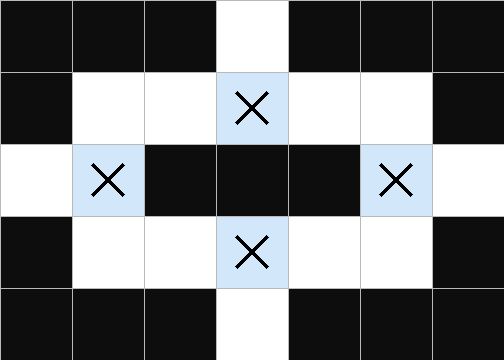
\includegraphics[width=0.36\textwidth]{figures/fig99_grid.png}

\medskip
\noindent\textbf{图 9.9\quad 带柱子的迷宫示例}
\end{center}

标着 X 的四个格位是路，但它们都绕着一个``柱子''——一块不与任何其他墙相连的墙——打转。在每个路口，goroutine 要么贴着柱子转，要么离开这个房间，但仍会制造出一个绕房间探索的分支。这意味着这样一个房间会制造出数不清的 goroutine，这对我们的计算机非常有害。我们可以要求用户提供无环迷宫，但也可以试着把这事当作探索的一部分来处理。

最后，我们确实解出了迷宫，但如果还能展示中间步骤岂不更好？这里，我们要把穿越迷宫的过程做成动画，产出一张漂亮的探索过程 GIF 文件。

% SOURCE_PDF_PAGE: 179
\subsection{克服环约束}

本章开头我们给自己立了规矩：迷宫绝不能有环。如果把它看成图，它就是一棵树——每个节点只有一条路径通向它。

如果去掉这条约束，通向宝藏的路径就可能有很多条。本章的目标并不是找最短路径。要找最短路，就得通过赋权值追踪每个像素到入口的距离，这可以用 RGBA 像素值的递增来实现。本节我们想尝试的只是找出其中一个解，并避免多次穿过相同的像素。

\subsubsection*{策略}

因为我们不想让任何 goroutine 探索之前已被探索过的像素——无论是它自己还是别的 goroutine 探索过的——我们要把这些像素当作正在探索像素的非候选邻居。为此，一个简单的技巧是：探索到它们时就把它们标记为已探索。先在 palette 结构里定义一个 explored 值：

\begin{gocode}[]
type palette struct {
    ...
    solution    color.RGBA
    explored    color.RGBA
}
\end{gocode}

接着，让 \texttt{defaultPalette} 函数为这个字段返回一个值（不同于 \texttt{palette.path} 的值）。然后，在 \texttt{explore} 函数里，我们要做的就是把正在探索的像素涂色，瞧，成了！

% SOURCE_PDF_PAGE: 180
\begin{gocode}[title={代码清单 9.30 \texttt{explore.go}：停止探索一条路径}]
func (s *Solver) explore(pathToBranch *path) {
    if pathToBranch == nil {
        // This is a safety net. It shouldn't be used,
        // but when it's needed, at least it's there.
        return
    }
    pos := pathToBranch.at
    for {
        s.maze.Set(pos.X, pos.Y, s.palette.explored) #1
        select {
\end{gocode}

\begin{codeannotations}
\item 把当前像素涂成已探索
\end{codeannotations}

\begin{center}
\begin{minipage}{0.52\textwidth}
  \centering

\includegraphics[width=0.78\linewidth]{figures/maze50_solved_render_hd.png}
\par\medskip
{\small\textbf{图 9.10\quad 解出的迷宫示例，已探索像素着色}}\par
\end{minipage}
\end{center}

从现在起，已探索的像素不会再成为候选——因为它不再是 \texttt{s.palette.path} 的颜色。现在运行程序，你应当会看到一幅解和已探索路径都着了色的图像，如图 9.10 所示。

\subsubsection*{实现陷阱}

且慢——我们有好几个 goroutine，而我们要每一个都去修改图像中某个像素的内容——这是数据竞争大开方便之门。在这个场景里这是个问题吗？有人可以辩称：在这种情形下这不是问题，因为无论哪个 goroutine
% SOURCE_PDF_PAGE: 181
抢先到场，结果都一样——每个 goroutine 会在那个像素写入相同的内容。任何被覆写或部分写入的值我们都能接受。但这完全错了。

\begin{infobox}{定义}
竞争条件（race condition）指的是未定义行为。不惜一切代价避免它。
\end{infobox}

根本不存在``良性竞争条件''这种东西。即便在刚才提到的情形里，同样的结果也不会出现，因为未定义行为意味着内存可能在别处被破坏，或者代码可能意外触发一颗炸弹。我们不知道。它是未定义的。编译器在把我们的代码翻译成机器语言时做了许多假设，其中之一就是：不存在数据竞争。

\subsection{让探索动起来}

我们知道自己的解能抵达宝藏。也有日志告诉我们找到了哪些死胡同。但这太不直观了，既然这是一章关于图像的内容，不如把它变得好玩些！

本节的目标是在我们穿越迷宫的过程中生成一列帧。每帧应展示给定时刻的探索状态。为此我们将用另一种图像格式——图形交换格式（GIF）——它可以用于动画（尽管这并非它最初的设计）。暂且不争论这个格式名字怎么念（至少在这章的有声书版出来之前），值得了解的是：一个 GIF 可以包含不止一个光栅帧。我们可以在单个 GIF 文件里编码多个帧，并且可以为每帧指定展示时长。这些时长
% SOURCE_PDF_PAGE: 182
以百分之一秒为单位，这是最接近屏幕刷新率的单位。既然决定要展示探索状态，该怎么做？

\subsubsection*{向 GIF 添加帧}

好，首先，我们需要能追踪到目前为止探索过的像素，这正是我们在 9.6.1 节所做的。其次，我们需要在探索的特定时刻添加帧——也就是带着当前已探索像素的图像。先给 Solver 结构加一个新字段，用标准库 \texttt{image/gif} 里的类型来持有 GIF：

\begin{gocode}[]
type Solver struct {
    ...
    animation      *gif.GIF
}
\end{gocode}

我们想什么时候给探索拍快照？如果用时间单位回答——比如每毫秒一帧——那么输出会随程序在不同电脑上跑得快慢而不同。否则，也可以考虑每发现 10 个新像素就展示一次状态。这虽然可行，但迷宫一大问题就严重了。假设迷宫含 40\% 的路径像素：在 10×10 的迷宫里约有 40 个路径像素可探索——那会做出一个 4 帧的 GIF。可是在 1000×1000 的迷宫里，约有 400000 个像素要探索，得到一个 40000 帧的 GIF。这样的文件一来非常重，二来如果每帧给百分之一秒的展示时间，最坏情况下要超过 6 分钟才能把探索放完。

% SOURCE_PDF_PAGE: 183
换个思路：我们干脆规定，如果探索整座迷宫，最终的 GIF 就要 30 帧长。这是个人为定的数，但做出来的动画不会太长。这意味着每探索 (总可探索像素)/(30 像素) 个像素，就要打印一次探索状态。我们需要为动画统计所有可探索像素，那就在新文件 \texttt{animation.go} 里写个函数吧。

\begin{gocode}[title={代码清单 9.31 \texttt{animation.go}：统计所有可探索像素}]
// countExplorablePixels scans the maze and counts the number
// of pixels that are not walls.
func (s *Solver) countExplorablePixels() int {
    explorablePixels := 0
    for row := 0; row < s.maze.Bounds().Dy(); row++ { #1
        for col := 0; col < s.maze.Bounds().Dx(); col++ { #2
            if s.maze.RGBAAt(col, row) != s.palette.wall { #3
                explorablePixels++
            }
        }
    }
    return explorablePixels
}

#1 The outer loop is on rows.
#2 The inner loop is on columns.
#3 Count path + treasure + entrance
\end{gocode}

\begin{codeannotations}
\item 外层循环在行上
\item 内层循环在列上
\item 统计路径 + 宝藏 + 入口
\end{codeannotations}

在 9.6.1 节里，我们遇到新的未探索像素时增加了一个操作——把它涂色。这里，我们想遇到新像素时再干点别的事。这需要把这些动作重构为 Solver 结构上的一个方法，不妨叫 \texttt{registerExploredPixel}。这个函数会把已探索像素涂色，并且根据已探索的数量，把帧添加进动画。然而，给像素涂色花不了多久，把帧添加进动画却意味着复制整幅图像，可能耗时很长。我们不想让这种复制阻塞任何探索进程，这意味着要让探索者异步地发送``有新像素待注册''的通知。

% SOURCE_PDF_PAGE: 184
Go 里做异步调用主要有两种方式。第一种是放进 goroutine 里调用：

\begin{gocode}[]
go s.registerExploredPixel(pos)
\end{gocode}

这完全可行，但我们必须自问：会不会发生竞争条件？归根结底，这个方法将需要显式使用互斥锁。但关于 goroutine 之间的通信我们说过什么来着？答案引出第二种做法，也是我们在此要用的：用一个通道，探索者把想注册的像素发送进去。这样一来，\texttt{registerExploredPixel} 从通道接收像素。只要我们逐一处理从通道读出的像素，就不需要互斥锁。把这个通道加进 Solver 结构吧。别忘了在 \texttt{New} 函数里初始化它：

\begin{gocode}[]
type Solver struct {
    ...
    exploredPixels chan image.Point
    animation      *gif.GIF
}
\end{gocode}

探索者的无限 for 循环可以更新为：要么在 quit 通道因找到解而关闭时中止，要么发送一个像素去注册并继续探索，如下面的清单所示。

% SOURCE_PDF_PAGE: 185
\begin{gocode}[title={代码清单 9.32 \texttt{explore.go}：把像素注册为已探索}]
func (s *Solver) explore(pathToBranch *path) { #1
    ...
    for {
        // Let's first check whether we should quit.
        select {
        case <-s.quit:
            return
        case s.exploredPixels <- pos: #1
            // Continue the exploration.
        }
    }
    ...
}

#1 Replaces the previous default case
\end{gocode}

\begin{codeannotations}
\item 替换先前的 default 分支
\end{codeannotations}

现在可以编写负责注册已探索像素的函数了，如代码清单 9.33 所示。要知道该多久写一帧，我们定义 \texttt{totalExpected­Frames} 为输出 GIF 想要的帧数——比方说最多 30 帧。我们不会精确得到 30 帧，因为我们不会探索每个像素。接着统计可探索像素的总数，然后用 for-select 模式持续运行，直到被告知退出。

每收到一个新探索像素的位置，我们就把它涂色、给已探索计数器加一，并在达到阈值时画一帧。

% SOURCE_PDF_PAGE: 186
\begin{gocode}[title={代码清单 9.33 \texttt{animation.go}：实现 \texttt{registerExploredPixels}}]
// registerExploredPixels registers positions as explored on the image,
// and, if we reach a threshold, adds the frame to the output GIF.
func (s *Solver) registerExploredPixels() {
    const totalExpectedFrames = 30
    explorablePixels := s.countExplorablePixels() #1
    pixelsExplored := 0
    for {
        select {
        case <-s.quit: #2
            return
        case pos := <-s.exploredPixels: #3
            s.maze.Set(pos.X, pos.Y, s.palette.explored) #4
            pixelsExplored++
            if pixelsExplored%(explorablePixels/totalExpectedFrames) == 0 {
                s.drawCurrentFrameToGIF()
            }
        }
    }
}

#1 Checks how many pixels are explorable
#2 Checks whether we should quit first
#3 Reads positions that have been explored
#4 Paints explored pixels
\end{gocode}

\begin{codeannotations}
\item 检查有多少像素可探索
\item 先检查是否应当退出
\item 读取已探索的位置
\item 把已探索像素涂色
\end{codeannotations}

现在来讨论 \texttt{drawCurrentFrameToGIF} 方法：它做什么、我们怎么画帧。首先，看看 \texttt{go doc gif.GIF.Image} 就会发现，GIF 结构使用的是调色板图像（paletted image）切片。这是一种压缩算法：图像用到的每种颜色存进一个调色板，每个像素不再用经典的 RGBA 值编码，而是用它颜色在调色板中的键编码。调色板的颜色数通常远少于整个 RGBA 光谱能提供的，这有时会导致结果图像出现压缩伪影。

创建调色板图像相当直接，因为 Go 有一个 \texttt{image/color/palette} 包，它只提供两个调色板——Plan9 和 WebSafe（还贴心地提到``早期版本的 Netscape Navigator''）。这里的选择权在你。我们还得决定：GIF 动画是与初始迷宫同尺寸，还是固定尺寸。与输入图像同尺寸更简单，但会让
% SOURCE_PDF_PAGE: 187
大多数 GIF 过小或过大。让帧与迷宫尺寸不同就需要像素插值，稍后几行就会看到。为了本章的目的，我们给每帧取固定宽度 500 像素、高度按输入图像像素的相同比例：

\begin{gocode}[]
const gifSize = 500
frame := image.NewPaletted(image.Rect(0, 0, gifSize, gifSize*s.maze.Bounds().Dy()/s.
maze.Bounds().Dx()), palette.Plan9)
\end{gocode}

在代码里使用 \texttt{image/color/palette} 会引起冲突！我们包里已经有一个叫 \texttt{palette} 的类型，它定义墙和路应当是什么颜色。通过给导入起别名，我们可以轻松化解这个冲突。

\begin{infobox}{注意}
在 Go 里，给导入起别名有时很有用。这里我们会用 \texttt{import plt "image/color/palette"}。给导入起别名时，最好用与原包名相似的别名，以保持代码清晰。
\end{infobox}

我们创建了一块空画布，下面把已探索迷宫的当前状态画上去。遗憾的是，Go 的 \texttt{image/draw} 包不支持缩放图像，因此也不支持任何插值。我们得用 \texttt{golang.org/x/image/draw}——它的功能更全的版本。这个包提供了 \texttt{golang.org/x/image/draw.Scaler} 接口，可以把输入图像的一个矩形区域缩放为输出图像的一个矩形区域。\texttt{golang.org/x/image/draw} 暴露了三个实现 Scaler 接口的类型：\texttt{Nearest­Neighbor}、\texttt{CatmullRom} 和 \texttt{ApproxBiLinear}。出于本章的目的，我们坚持用 \texttt{NearestNeighbor}，因为它不会把像素边缘弄糊：

\begin{gocode}[]
draw.NearestNeighbor.Scale(frame, frame.Rect, s.maze, s.maze.Bounds(),
draw.Over, nil)
\end{gocode}

% SOURCE_PDF_PAGE: 188
最后，把帧添加进我们的 GIF 图像。这三项操作可以写进一个由 \texttt{markPixelExplored} 调用的方法。

\begin{gocode}[title={代码清单 9.34 \texttt{animation.go}：把帧画到 GIF 上}]
package solver

import (
    "image"
    plt "image/color/palette" #1
    "golang.org/x/image/draw"
)

// ...
// drawCurrentFrameToGIF adds the current state of the maze
// as a frame of the animation.
func (s *Solver) drawCurrentFrameToGIF() {
    const (
        // gifWidth is the width of the generated GIF.
        gifWidth = 500
        // frameDuration is the duration in hundredth of a second
        // of each frame.
        // 20 hundredths of a second per frame means 5 frames per second.
        frameDuration = 20
    )
    // Create a paletted frame that has the same ratio as the input image
    frame := image.NewPaletted(image.Rect(0, 0, gifSize,
        gifWidth*s.maze.Bounds().Dy()/s.maze.Bounds().Dx()), plt.Plan9)
    // Convert RGBA to paletted
    draw.NearestNeighbor.Scale(
        frame, frame.Rect, s.maze, s.maze.Bounds(), draw.Over, nil)
    s.animation.Image = append(s.animation.Image, frame)
    s.animation.Delay = append(s.animation.Delay, frameDuration)
}

#1 Aliases the import to avoid conflict with the type palette
\end{gocode}

\begin{codeannotations}
\item 给导入起别名，避免与类型 \texttt{palette} 冲突
\end{codeannotations}

现在我们有了一个单独的 goroutine 负责更新图像像素的值，它随着像素从通道到来而逐个处理。别忘了在 Solve 里启动这个 \texttt{registerExploredPixels} 方法。现在我们有两个想启动的``监听'' goroutine——\texttt{listenToBranches} 和 \texttt{registerExploredPixels}。要把两者都启动、并在它们返回后同步，可以用 \texttt{sync.WaitGroup}。

% SOURCE_PDF_PAGE: 189
\begin{gocode}[title={代码清单 9.35 \texttt{solver.go}：在 \texttt{Solve} 里启动监听者}]
func (s *Solver) Solve() error {
    // ...
    log.Printf("starting at %v", entrance)
    s.pathsToExplore <- &path{previousStep: nil, at: entrance}
    wg := sync.WaitGroup{}
    wg.Add(2)
    defer wg.Wait() #1
    go func() { #2
        defer wg.Done()
        // Launch the goroutine in charge of drawing the GIF image.
        s.registerExploredPixels()
    }()
    go func() { #3
        defer wg.Done()
        // Listen for new paths to explore.
        // This only returns when the maze is solved.
        s.listenToBranches()
    }()
    return nil
}

#1 Solve won't return unless both goroutines are done.
#2 One goroutine to register explored pixels
#3 One goroutine to explore new branches
\end{gocode}

\begin{codeannotations}
\item 两个 goroutine 不都完成，\texttt{Solve} 就不返回
\item 一个 goroutine 注册已探索像素
\item 一个 goroutine 探索新分支
\end{codeannotations}

\subsubsection*{生成 GIF 文件}

现在我们已经把帧加进了 GIF。每帧都是从正在探索的迷宫逐像素复制来的。

接下来，把 GIF 文件画出来。为此，只需在代码里知道``可以打印了''的位置接上一个写出动画输出图像的函数调用。现有的 \texttt{SaveSolution} 函数是绝佳选择，因为它已经负责写一个输出文件了。我们在那里调用一个新方法来画最终的 GIF。

% SOURCE_PDF_PAGE: 190
\begin{gocode}[title={代码清单 9.36 \texttt{imagefile.go}：生成 GIF 文件}]
func (s *Solver) SaveSolution(outputPath string) error {
     // ...
    gifPath := strings.Replace(outputPath, "png", "gif", -1)
    err = s.saveAnimation(gifPath)
    if err != nil {
        return fmt.Errorf(...)
    }
    return nil
}

// saveAnimation writes the gif file.
func (s *Solver) saveAnimation(gifPath string) error {
    outputImage, err := os.Create(gifPath)
    if err != nil {
        return fmt.Errorf(...)
    }
    defer func() {
        if closeErr := outputImage.Close(); closeErr != nil {
            // Return err and closeErr, in worst case scenario.
            err = errors.Join(err,
                fmt.Errorf("unable to close file: %w", closeErr))
        }
    }()
    log.Printf("animation contains %d frames\n", len(s.animation.Image))
    err = gif.EncodeAll(outputImage, s.animation)
    if err != nil {
        return fmt.Errorf("unable to encode gif: %w", err)
    }
    return nil
}
\end{gocode}

这段代码与 PNG 图像编码的代码非常相似。现在，让我们运行程序：

\begin{shellcode}[]
> go run . mazes/maze50_50.png solution.png
2023/10/18 11:42:57 INFO Solving maze "mazes/maze50_50.png" and saving it
as "solution.png"
2023/10/18 11:42:57 INFO starting at (0,25)
2023/10/18 11:43:00 INFO Treasure found: (18,0)!
2023/10/18 11:43:00 INFO the treasure has been found, worker going to sleep
2023/10/18 11:43:00 INFO animation contains 30 frames
\end{shellcode}

这应当会生成 \texttt{solution.png} 图像以及一个 \texttt{solution.gif} 文件。打开这个文件，看看迷宫是如何被探索的。你注意到什么了吗？解显示得并不清楚——如果它有显示的话——而且循环马上重新开始。要是能把
% SOURCE_PDF_PAGE: 191
解加进帧列表、并让这最后一帧打印得更久一些，那就好了。

在 9.4 节，我们把解的涂色加进了 \texttt{SaveSolution} 方法。现在需要对 GIF 做点事，我们也许想要一个专门的方法，把这段逻辑从写文件的代码挪到 Solver 里。让我们为本章写下最后几行代码。先把 Solver 存储的图像里入口与解之间的像素涂色，然后向 GIF 添加最后一帧（包含涂了解的像素），如下面的清单所示。通过设一个更长的值，我们确保最后一帧会展示得足够久，好让人细细欣赏。

\begin{gocode}[title={代码清单 9.37 \texttt{solver.go}：保存解，为探索收尾}]
func (s *Solver) Solve() error {
    // ...
    wg.Wait()
    s.writeLastFrame()
    return nil
}

// writeLastFrame writes the last frame of the gif,
// with the solution highlighted.
func (s *Solver) writeLastFrame() {
    stepsFromTreasure := s.solution
    // Paint the path from entrance to the treasure.
    for stepsFromTreasure != nil { #1
        s.maze.Set(stepsFromTreasure.at.X, stepsFromTreasure.at.Y,
            s.palette.solution)
        stepsFromTreasure = stepsFromTreasure.previousStep
    }
    const solutionFrameDuration = 300 // 3 seconds
    // Add the solution frame, with the coloured path, to the output gif.
    s.drawCurrentFrameToGIF()  #2
    s.animation.Delay[len(s.animation.Delay)-1] = solutionFrameDuration
}

#1 Makes sure the treasure is found
#2 Draws the final frame of the GIF with a longer duration
\end{gocode}

\begin{codeannotations}
\item 确保宝藏被找到
\item 画出 GIF 的最后一帧，并给予更长的展示时间
\end{codeannotations}

重新运行程序，打开 GIF。你可以调整帧时长或帧数，
% SOURCE_PDF_PAGE: 192
来获得你真正想要的观感。遗憾的是，我们没法把 GIF 放进书里——把你的 GIF 分享给朋友们吧！

\section*{小结}

\begin{itemize}
\item 在计算机科学中，2D 图像的主要类型是光栅图像和矢量图像。
\item 矢量图像用于字体和标志、信息图或图标。矢量图像缩放性极好——放大也看不到任何伪影。
\item 我们使用的另一半图像是光栅图像——像素组成的 2D 网格。图像的每个像素都有一种颜色，可以用 RGBA 颜色模型表示（但也可能以其他颜色模型编码，比如 JPEG 图像的 YCbCr）。颜色的值既可以用来编码物理信息，比如物体发出的红、绿、蓝频率光的强度（如一张花的照片），也可以编码任何数值信息（例如人口密度）。此外，还可以用调色板来表示同属一类的区域，比如地图上每个国家有自己的颜色。
\item \texttt{image/png} 包用于把文件 Decode 成 \texttt{image.Image}。这个 Image 经常被类型断言为 RGBA 或 NRGBA。要编码图像，请用你想把图像编码成的那个包的 Encode 函数——可选的是 gif、jpeg 和 png。其他格式需要第三方库。
\item 图像通常把 (0, 0) 位置的像素放在左上角。然而，有些图像的 (0, 0) 可能在任何一个角。这完全取决于图像格式和图像元数据。请使用 \texttt{image} 包返回的内容来迭代图像的像素。
% SOURCE_PDF_PAGE: 193
\item 可以用 \texttt{.At()} 方法访问 \texttt{image.Image} 中像素的值。它返回一个 \texttt{color.Color()}，你必须把它转换成 \texttt{color.RGBA}。使用 \texttt{image.RGBA} 时，可以改用 \texttt{RGBAAt()}，它返回的 \texttt{color.RGBA} 可直接与已知值比较。
\item 要向 \texttt{image.RGBA} 写入像素，使用 \texttt{Set(x, y, rgba)} 方法。
\item 扫描整幅图像时，使用两层嵌套循环——最外层遍历行，最内层遍历列。这对所有扫描线格式的性能都有好处。
\item 当无法使用全局常量时，用一个返回配置值的函数比用全局变量稍显干净。出于安全考虑，避免暴露全局变量：其他代码可能会改掉它们。
\item 向一个无人读取的无缓冲通道写入是阻塞的。要么在 goroutine 里写，要么使用带缓冲通道——其大小应当是读取开始之前会写入那里的元素的最大数量。
\item 在循环里启动 goroutine 时，确保循环变量受到保护。循环变量可能是你从通道读出的消息、你遍历的映射的键或值，或者切片的元素。在循环内部启动 goroutine 时，保护 for 循环迭代器有三种常见方式：
  \begin{itemize}
  \item 使用保证这一点的 Go 版本（目前，这被认为是 Go 1.22）。
  \item 在循环里用另一个变量遮蔽（shadow）循环变量（通常，我们给新变量起与循环变量相同的名字）。
  \item 用一个把循环变量作为参数的匿名函数来启动 goroutine。
  \end{itemize}
% SOURCE_PDF_PAGE: 194
\item \texttt{select} 关键字允许一段代码监听多个通道。只要任一通道发布了消息，对应 case 语句里写的代码就会被执行。
\item 如果 select 中有多个 case 语句都就绪，Go 会随机挑一个。
\item select 的某个 case 语句常常充当返回条件。在服务器里尤其如此：一旦请求被取消，对该输入请求的处理就应当尽快结束。
\item for-select 无限循环的监听模式非常常见。通常，select 块的某个 case 会包含退出循环的条件。
\end{itemize}


\end{document}
